\documentclass{report}

\input{~/dev/latex/template/preamble.tex}
\input{~/dev/latex/template/macros.tex}

\title{\Huge{}}
\author{\huge{Nathan Warner}}
\date{\huge{}}
\pagestyle{fancy}
\fancyhf{}
\rhead{}
\fancyhead[R]{\itshape Warner} % Right header: Last Name
\fancyhead[L]{\itshape\leftmark}  % Right header: Section Name
\cfoot{\thepage}
\renewcommand{\headrulewidth}{0pt} % Remove the header line

% Change the title
\hypersetup{
	pdftitle={Math 2}
}


\begin{document}
    % \maketitle
        \begin{titlepage}
       \begin{center}
           \vspace*{1cm}
    
           \textbf{Comprehensive Compendium:} \\
            Calculus II, Calculus III, Newtonian Mechanics, Probability and Statistics
    
           \vspace{0.5cm}
            
                
           \vspace{1.5cm}
    
           \textbf{Nathan Warner}
    
           \vfill
                
                
           \vspace{0.8cm}
         
           
\includegraphics[width=0.4\textwidth]{~/niu/seal.png}
                
           Computer Science \\
           Northern Illinois University\\
           August 28,2023 \\
           United States\\
           
                
       \end{center}
    \end{titlepage}
    \tableofcontents
    \pagebreak \bigbreak \noindent
    \unsect{Calculus II}
    \bigbreak \noindent 

    \bigbreak \noindent 
    \subsection{Chapter 1 Definitions and Theorems}
    \bigbreak \noindent 
    \begin{itemize}
        \item \textbf{Mean Value Theorem For Integrals}}: If  $f(x)$ is continuous over an interval  [a,b], then there is at least one point  $c\in[a,b]$ such that 
            \begin{align*}
                f(c) = \frac{1}{b-a}\int f(x)\ dx
            .\end{align*}
        \item \textbf{Integrals resulting in inverse trig functions}}:
            \begin{enumerate}
                \item \begin{align*}
                        \int \frac{dx}{\sqrt{a^{2}-x^{2}}} = \sin^{-1}{\frac{x}{\abs{a}}} + C
                    .\end{align*}
                \item \begin{align*}
                        \int \frac{dx}{a^{2}+x^{2}} = \frac{1}{a}\tan^{-1}{\frac{x}{a}} + C
                    .\end{align*}
                \item \begin{align*}
                        \int \frac{dx}{x\sqrt{x^{2}-a^{2}}} = \frac{1}{\abs{a}}\sec^{-1}{\frac{\abs{x}}{a}} + C
                    .\end{align*}
            \end{enumerate}
    \end{itemize}

    % \pagebreak \bigbreak \noindent 
    % \subsection{Chapter 2 Key Terms / Ideas}
    % \bigbreak \noindent 
    % \begin{itemize}
    %     \item \textbf{Finding limits of integration for region between two functions}}: Usually, we want our limits of integration to be the points where the functions intersect
    %     \item \textbf{"complex region"}}: between curves usually refers to an area that is not easily described by a single, continuous function over the interval of interest.
    %     \item \textbf{compound regions}}: are regions bounded by the graphs of functions that cross one another
    %     \item \textbf{Cross-section:}}: The intersection of a plane and a solid object.
    %     \item \textbf{cylinder}}: is a three-dimensional shape that has two parallel, congruent bases connected by a curved surface. The bases are usually circles, but they can be other shapes as well
    %     \item \textbf{"axis" of the cylinder.}}:
    %     \item \textbf{Slicing method:}}: A method of calculating the volume of a solid that involves cutting the solid into pieces, estimating the volume of each piece, then adding these estimates to arrive at an estimate of the total volume; as the number of slices goes to infinity, this estimate becomes an integral that gives the exact value of the volume.
    %     \begin{enumerate}
    %         \item Examine the solid and determine the shape of a cross-section of the solid. It is often helpful to draw a picture if one is not provided.
    %         \item Determine a formula for the area of the cross-section.
    %         \item Integrate the area formula over the appropriate interval to get the volume.
    %     \end{enumerate}
    %     \item \textbf{Solid of revolution:}}: A solid generated by revolving a region in a plane around a line in that plane.
    %     \item \textbf{Disk method:}}: A special case of the slicing method used with solids of revolution when the slices are disks.
    %     \item \textbf{Washer (Annuli)}}: is a disk with holes in the center.
    %     \item \textbf{Washer method:}}: A special case ofthe slicing method used with solids of revolution when the slices are washers.
    %     \item \textbf{Method of cylindrical shells:}}: A method of calculating the volume of a solid of revolution by dividing the solid into nested cylindrical shells; this method is different from the methods of disks or washers in that we integrate with respect to the opposite variable.
    %     % \item \textbf{axis of the cylinder}}:.
    %      \item \textbf{Arc length:}}: The arc length of a curve can be thought of as the distance a person would travel along the path of the curve.
    %     \item \textbf{Surface area:}}: The surface area of a solid is the total area of the outer layer of the object; for objects such as cubes or bricks, the surface area of the object is the sum of the areas of all of its faces.
    %     % \item \textbf{Catenary:}}: A curve in the shape of the function \(y = a \cosh(x/a)\) is a catenary; a cable of uniform density suspended between two supports assumes the shape of a catenary.
    %     % \item \textbf{Center of mass:}}: The point at which the total mass of the system could be concentrated without changing the moment.
    %     % \item \textbf{Centroid:}}: The centroid of a region is the geometric center of the region; laminas are often represented by regions in the plane; if the lamina has a constant density, the center of mass of the lamina depends only on the shape of the corresponding planar region; in this case, the center of mass of the lamina corresponds to the centroid of the representative region.
    %     % \item \textbf{Density function:}}: A density function describes how mass is distributed throughout an object; it can be a linear density, expressed in terms of mass per unit length; an area density, expressed in terms of mass per unit area; or a volume density, expressed in terms of mass per unit volume; weight-density is also used to describe weight (rather than mass) per unit volume.
    %     % \item \textbf{Doubling time:} If a quantity grows exponentially, the doubling time is the amount of time it takes the quantity to double, and is given by \(\frac{\ln 2}{k}}:\).
    %     % \item \textbf{Exponential decay:} Systems that exhibit exponential decay follow a model of the form \(y = y_0 e^{-kt}}:\).
    %     % \item \textbf{Exponential growth:} Systems that exhibit exponential growth follow a model of the form \(y = y_0 e^{kt}}:\).
    %     % \item \textbf{Frustum:}}: A portion of a cone; a frustum is constructed by cutting the cone with a plane parallel to the base.
    %     % \item \textbf{Half-life:} If a quantity decays exponentially, the half-life is the amount of time it takes the quantity to be reduced by half. It is given by \(\frac{\ln 2}{k}}:\).
    %     % \item \textbf{Hooke's Law:}}: This law states that the force required to compress (or elongate) a spring is proportional to the distance the spring has been compressed (or stretched) from equilibrium; in other words, \(F = kx\), where \(k\) is a constant.
    %     % \item \textbf{Hydrostatic pressure:}}: The pressure exerted by water on a submerged object.
    %     % \item \textbf{Lamina:}}: A thin sheet of material; laminas are thin enough that, for mathematical purposes, they can be treated as if they are two-dimensional.
    %     % \item \textbf{Moment:} If \(n\) masses are arranged on a number line, the moment of the system with respect to the origin is given by \(M = \sum_{i=1}^{n} m_i x_i\); if, instead, we consider a region in the plane, bounded above by a function \(f(x)\) over an interval \([a, b]\), then the moments of the region with respect to the \(x\)- and \(y\)-axes are given by \(M_x = \rho \int_{a}^{b} \frac{[f(x)]^2}{2} dx\) and \(M_y = \rho \int_{a}^{b}}: x f(x) dx\), respectively.
    %     % \item \textbf{Symmetry principle:}}: The symmetry principle states that if a region \(R\) is symmetric about a line \(l\), then the centroid of \(R\) lies on \(l\).
    %     % \item \textbf{Theorem of Pappus for volume:}}: This theorem states that the volume of a solid of revolution formed by revolving a region around an external axis is equal to the area of the region multiplied by the distance traveled by the centroid of the region.
    %     % \item \textbf{Work:}}: The amount of energy it takes to move an object; in physics, when a force is constant, work is expressed as the product of force and distance.
    % \end{itemize}

    \pagebreak \bigbreak \noindent 
    \subsection{Chapter 2 Definitions and Theorems}
    \bigbreak \noindent 
    \begin{itemize}

        \item \textbf{Area between two curves, integrating on the x-axis}}:
            \begin{align}
                A = \int_{a}^{b} [f(x) - g(x)] \, dx
            \end{align}
            Where $f(x) \geq g(x)$
            \begin{align*}
                A = \int_{a}^{b}\ [g(x) - f(x)]\ dx
            .\end{align*}
            for $g(x) \geq f(x)$

        \item \textbf{Area between two curves, integrating on the y-axis}}:
            \begin{align}
                A = \int_{c}^{d} [u(y) - v(y)] \, dy
            \end{align}

        \item \textbf{Areas of compound regions}}:
            \begin{align*}
                \int_{a}^{b}\ \abs{f(x)-g(x)}\ dx 
            .\end{align*}
        \item \textbf{Area of complex regions}}:
            \begin{align*}
                \int_{a}^{b}\ f(x)\ dx + \int_{b}^{c}\ g(x)\ dx
            .\end{align*}
        \item \textbf{Slicing Method}}:
            \begin{align*}
                V(s) = \summation{n}{i=1}\ A(x_{i}^{*})\ \Delta x  = \int_{a}^{b}\ A(x)\ dx
            .\end{align*}
        \item \textbf{Disk Method along the x-axis}}:
            \begin{align}
                V = \int_{a}^{b} \pi [f(x)]^2 \, dx
            \end{align}

        \item \textbf{Disk Method along the y-axis}}:
            \begin{align}
                V = \int_{c}^{d} \pi [g(y)]^2 \, dy
            \end{align}

        \item \textbf{Washer Method along the x-axis}}:
            \begin{align}
                V = \int_{a}^{b} \pi [(f(x))^2 - (g(x))^2] \, dx
            \end{align}

        \item \textbf{Washer Method along the y-axis}}:
            \begin{align}
                V = \int_{c}^{d} \pi [(u(y))^2 - (v(y))^2] \, dy
            \end{align}

        \item \textbf{Radius if revolved around other line (Washer Method)}}:
            \begin{align*}
                If:\ x=-k\\
                Then:\ r = Function + k
            .\end{align*}
            \begin{align*}
                If:\ x=k\\
                Then:\ r = k - Function
            .\end{align*}

        \item \textbf{Method of Cylindrical Shells (x-axis)}}:
            \begin{align}
                V = \int_{a}^{b} 2\pi x f(x) \, dx
            \end{align}

        \item \textbf{Method of Cylindrical Shells (y-axis)}}:
            \begin{align}
                V = \int_{c}^{d} 2\pi y g(y) \, dy
            \end{align}

        \item \textbf{Region revolved around other line (method of cylindrical shells):}}:
            \begin{align*}
                If:\ x=-k \\
                Then:\ V = \int_{a}^{b}\ 2\pi (x+k)(f(x))\ dx
            .\end{align*}
            \begin{align*}
                If:\ x=k \\
                Then:\ V = \int_{a}^{b}\ 2\pi (k-x)(f(x))\ dx
            .\end{align*}
        \item \textbf{A Region of Revolution Bounded by the Graphs of Two Functions (method cylindrical shells)}}:
            \begin{align*}
                V = \int_{a}^{b}\ 2\pi x\left[f(x)-g(x)\right]\ dx
            .\end{align*}

        \item \textbf{Arc Length of a Function of x}}:
            \begin{align}
                \text{Arc Length} = \int_{a}^{b} \sqrt{1 + [f'(x)]^2} \, dx
            \end{align}

        \item \textbf{Arc Length of a Function of y}}:
            \begin{align}
                \text{Arc Length} = \int_{c}^{d} \sqrt{1 + [g'(y)]^2} \, dy
            \end{align}

        \item \textbf{Surface Area of a Function of x (Around x)}}:
            \begin{align}
                \text{Surface Area} = \int_{a}^{b} 2\pi f(x) \sqrt{1 + [f'(x)]^2} \, dx
            \end{align}

        \item \textbf{Surface Area of a Function of x (Around y)}}:
            \begin{align}
                \text{Surface Area} = \int_{a}^{b} 2\pi x \sqrt{1 + [f'(x)]^2} \, dx \\
                \text{Or: } \int_{a}^{b}\ 2\pi u(y)\sqrt{1+(u^{\prime}(y))^{2}}\ dy
            \end{align}

        \item \textbf{Natural logarithm function}}:
            \begin{align}
                \ln x = \int_{1}^{x} \frac{1}{t} \, dt\
            \end{align}

        \item \textbf{Exponential function}}:
            \begin{align}
                y = e^x, \quad \ln y = \ln(e^x) = x\
            \end{align}

        \item \textbf{Logarithm Differentiation}}:
            \begin{align*}
                f^{\prime}(x) = f(x) \cdot \frac{d}{dx}\ln{\left(f^{\prime}(x)\right)}
            .\end{align*}
            \textbf{Note:} Use properties of logs before you differentiate whats inside the logarithm

            % \item \textbf{Mass of a one-dimensional object}}:
            % \begin{align}
            %     m = \int_{a}^{b} \rho(x) \, dx
            % \end{align}
            %
            % \item \textbf{Mass of a circular object}}:
            % \begin{align}
            %     m = \int_{0}^{r} 2\pi x \rho(x) \, dx
            % \end{align}
            %
            % \item \textbf{Work done on an object}}:
            % \begin{align}
            %     W = \int_{a}^{b} F(x) \, dx
            % \end{align}
            %
            % \item \textbf{Hydrostatic force on a plate}}:
            % \begin{align}
            %     F = \int_{a}^{b} \rho w(x) s(x) \, dx
            % \end{align}
            %
            % \item \textbf{Mass of a lamina}}:
            % \begin{align}
            %     m = \rho \int_{a}^{b} f(x) \, dx
            % \end{align}
            %
            % \item \textbf{Moments of a lamina}}:
            % \begin{align}
            %     M_x = \rho \int_{a}^{b} \frac{[f(x)]^2}{2} \, dx, \quad M_y = \rho \int_{a}^{b} x f(x) \, dx
            % \end{align}
            %
            % \item \textbf{Center of mass of a lamina}}:
            % \begin{align}
            %     \bar{x} = \frac{M_y}{m},\ \ \text{and}\ \  \bar{y} = \frac{M_x}{m}
            % \end{align}

    \end{itemize}


    % \pagebreak \bigbreak \noindent 
    % \subsection{Chapter 3 Key Terms}
    % \bigbreak \noindent 
    % \begin{itemize}
    %     \item \textbf{integration by parts}}: a technique of integration that allows the exchange of one integral for another using the formula 
    %     \item \textbf{integration table}}: a table that lists integration formulas.
    %     \item \textbf{power reduction formula}}: a rule that allows an integral of a power of a trigonometric function to be exchanged for an integral involving a lower power.
    %     \item \textbf{trigonometric integral}}: an integral involving powers and products of trigonometric functions.
    %     \item \textbf{trigonometric substitution}: an integration technique that converts an algebraic integral containing expressions of the form \( \sqrt{a^2 - x^2} \), \( \sqrt{a^2 + x^2} \), or \( \sqrt{x^2 - a^2}}: \) into a trigonometric integral.
    %     \item \textbf{partial fraction decomposition}}: a technique used to break down a rational function into the sum of simple rational functions.
    %     \item \textbf{improper integral}}: an integral over an infinite interval or an integral of a function containing an infinite discontinuity on the interval; an improper integral is defined in terms of a limit. The improper integral converges if this limit is a finite real number; otherwise, the improper integral diverges.
    %      % \item \textbf{absolute error}}: if \( B \) is an estimate of some quantity having an actual value of \( A \), then the absolute error is given by \( |A-B| \).
    %     % \item \textbf{computer algebra system (CAS)}}: technology used to perform many mathematical tasks, including integration.
    %     % \item \textbf{midpoint rule}}: a rule that uses a Riemann sum of the form 
    %     % \item \textbf{numerical integration}}: the variety of numerical methods used to estimate the value of a definite integral, including the midpoint rule, trapezoidal rule, and Simpson’s rule.
    %     % \item \textbf{relative error}}: error as a percentage of the absolute value, given by 
    %     % \item \textbf{Simpson’s rule}: a rule that approximates \( \int_{a}^{b} f(x) \, dx \) using the integrals of a piecewise quadratic function. The approximation \( S_n \) to \( \int_{a}^{b}}: f(x) \, dx \) is given by 
    %     % \item \textbf{trapezoidal rule}: a rule that approximates \( \int_{a}^{b}}: f(x) \, dx \) using trapezoids.
    % \end{itemize}
    %
    \pagebreak \bigbreak \noindent 
    \subsection{Chapter 3 Definitions and Theorems}
    \bigbreak \noindent 
    \begin{itemize}
        \item \textbf{Integration by parts formula}}: 
            \begin{align*}
                \int u \, dv &= uv - \int v \, du 
            .\end{align*}
        \item \textbf{Integration by parts for definite integral}}:
            \begin{align*}
                \int_{a}^{b} u \, dv &= uv\big|_{a}^{b} - \int_{a}^{b} v \, du
            \end{align*}
        \item \textbf{To integrate products involving  sin(ax), sin(bx), cos(ax), and  cos(bx), use the substitutions:}}:
            \begin{itemize}
                \item \textbf{Sine Products}}:
                    \begin{align*}
                        \sin(ax) \sin(bx) &= \frac{1}{2} \cos((a-b)x) - \frac{1}{2} \cos((a+b)x)
                    \end{align*}

                \item \textbf{Sine and Cosine Products}}:
                    \begin{align*}
                        \sin(ax) \cos(bx) &= \frac{1}{2} \sin((a-b)x) + \frac{1}{2} \sin((a+b)x)
                    \end{align*}

                \item \textbf{Cosine Products}}:
                    \begin{align*}
                        \cos(ax) \cos(bx) &= \frac{1}{2} \cos((a-b)x) + \frac{1}{2} \cos((a+b)x)
                    \end{align*}

                \item \textbf{Power Reduction Formula (sine)}}:
                    \begin{align*}
                        &\int \sin^{n}{x}\ dx = -\frac{1}{n}\sin^{n-1}{x}\cos{x} + \frac{n-1}{n}\int \sin^{n-2}{x}\ dx \\
                        &\int_{0}^{\frac{\pi}{2}}\ \sin^{n}{x}\ dx = \frac{n-1}{n}\int_{0}^{\frac{\pi}{2}}\ \sin^{n-2}{x}\ dx
                    .\end{align*}
                \item \textbf{Power Reduction Formula (cosine)}}:
                    \begin{align*}
                        &\int \cos^{n}{x}\ dx = \frac{1}{n}\cos^{n-1}{x}\sin{x} + \frac{n-1}{n}\int \cos^{n-2}{x}\ dx \\
                        &\int_{0}^{\frac{\pi}{2}}\ \cos^{n}{x}\ dx = \frac{n-1}{n}\int_{0}^{\frac{\pi}{2}}\ \cos^{n-2}{x}\ dx
                    .\end{align*}
                \item \textbf{Power Reduction Formula (secant)}}:
                    \begin{align*}
                        \int \sec^{n}{x}\ dx &= \frac{1}{n-1}\sec^{n-1}{x}\sin{x}+\frac{n-2}{n-1}\int \sec^{n-2}{x}\ dx \\
                        \int \sec^{n}{x}\ dx &= \frac{1}{n-1}\sec^{n-2}{x}\tan{x}+\frac{n-2}{n-1}\int \sec^{n-2}{x}\ dx
                    \end{align*}

                \item \textbf{Power Reduction Formula (tangent)}}:
                    \begin{align*}
                        \int \tan^n x \, dx &= \frac{1}{n-1} \tan^{n-1}x - \int \tan^{n-2}x \, dx
                    \end{align*}
            \end{itemize}
        \item \textbf{Trigonometric Substitution}}:
            \begin{itemize}
                \item $\sqrt{a^{2} - x^{2}}$ use $x =a\sin{\theta }$ with domain restriction $\bigg[-\frac{\pi}{2},\frac{\pi}{2}\bigg] $
                \item $\sqrt{a^{2} + x^{2}}$ use $x=a\tan{\theta}$ with domain restriction $\left(-\frac{\pi}{2}, \frac{\pi}{2}\right)$
                \item $\sqrt{x^{2} - a^{2}}$ use $x =a\sec{\theta}$ with domain restriction $\bigg[0,\frac{\pi}{2}\bigg) \cup \bigg[\pi,\frac{3\pi}{2}\bigg)$ 
            \end{itemize}

        \item \textbf{Steps for fraction decomposition}}:
            \begin{enumerate}
                \item Ensure $deg(Q) < deg(P)$, if not, long divide
                \item Factor denominator
                \item Split up fraction into factors
                \item Multiply through to clear denominator
                \item Group terms and equalize
                \item Solve for constants
                \item Plug constants into split up fraction
                \item Compute integral
            \end{enumerate}

        \item \textbf{Solving for constants}}:
            Either:
            \begin{itemize}
                \item Plug in values (often the roots)
                \item Equalize 
            \end{itemize}
        \item \textbf{Cases for partial fractions}}:
            \begin{itemize}
                \item Non repeated linear factors
                \item Repeated linear factors
                \item Nonfactorable quadratic factors
            \end{itemize}
        \item \textbf{Midpoint rule}}:
            \begin{align*}
                M_{n} = \summation{n}{i=1}\ f(m_{i})\ \Delta x 
            .\end{align*}
        \item \textbf{Absolute error}}:
            \begin{align*}
                err = \bigg|\text{Actual} - \text{Estimated}\bigg|
            .\end{align*}
        \item \textbf{Relative error}}:
            \begin{align*}
                err = \bigg|\frac{\text{Actual} - \text{Estimated}}{\text{Actual}}\bigg| \cdot 100\%
            .\end{align*}
        \item \textbf{Error upper bound for midpoint rule}}:
            \begin{align*}
                E_{M} \leq \frac{M(b-a)^3}{24n^2}
            \end{align*}
            Where $M$ is the maximum value of the second derivative
        \item \textbf{Trapezoidal rule}}:
            \begin{align*}
                T_n \frac{1}{2} \Delta x \left( f(x_0) + 2f(x_1) + 2f(x_2) + \cdots + 2f(x_{n-1}) + f(x_n) \right)
            \end{align*}
        \item \textbf{Error upper bound for trapezoidal rule}}:
            \begin{align*}
                E_{T} \leq \frac{M(b-a)^3}{12n^2}
            \end{align*}
            Where $M$ is the maximum value of the second derivative
        \item \textbf{Simpson’s rule}}:
            \begin{align*}
                S_n = \frac{\Delta x}{3} \left( f(x_0) + 4f(x_1) + 2f(x_2) + 4f(x_3) + 2f(x_4) + 4f(x_5) + \cdots + 2f(x_{n-2}) + 4f(x_{n-1}) + f(x_n) \right)
            \end{align*}
        \item \textbf{Error upper bound for Simpson’s rule}}:
            \begin{align*}
                E_{S} \leq \frac{M(b-a)^5}{180n^4}
            \end{align*}
            Where $M$ is the maximum value of the fourth derivative
        \item \textbf{Finding $n$ with error bound functions}}:
            \begin{enumerate}
                \item Find $f^{\prime\prime}(x)$
                \item Find maximum values of $f^{\prime\prime}(x)$ in the interval
                \item Plug into error bound function 
                \item Set value $\leq$ desired accuracy (ex: 0.01)
                \item Solve: 
                \item If we were to truncate, we would use the ceil function $\ceil*{n}$ DO NOT FLOOR
            \end{enumerate}
        \item \textbf{Improper integrals (Infinite interval)}}:
            \begin{itemize}
                \item $\int_{a}^{+\infty}\ f(x)\ dx  = \lim\limits_{t \to +\infty}{\int_{a}^{t}\ f(x)\ dx}$  
                \item $\int_{-\infty}^{b}\ f(x)\ dx = \lim\limits_{t \to -\infty}{\int_{t}^{b}\ f(x)\ dx}$ 
                \item $\int_{-\infty}^{+\infty}\ f(x)\ dx = \int_{-\infty}^{0}\ f(x)\ dx + \int_{0}^{+\infty}\ f(x)\ dx$
            \end{itemize}
        \item \textbf{Improper integral (discontinuous)}}:
            \begin{itemize}
                \item Let $f(x)$ be continuous on $[a,b)$, then;
                    \begin{align*}
                        \int_{a}^{b}\ f(x)\ dx = \lim\limits_{t \to b^{-}}{\int_{a}^{t}\ f(x)\ dx}\
                    .\end{align*}
                \item Let $f(x)$ be continuous on $(a,b]$, then;
                    \begin{align*}
                        \int_{a}^{b}\ f(x)\ dx = \lim\limits_{t \to b^{+}}{\int_{t}^{b}\ f(x)\ dx}\
                    .\end{align*}
                    In each case, if the limit exists, then the improper integral is said to converge. If the limit does not exist, then the improper integral is said to diverge.
                \item Let $f(x)$ be continuous on $[a,b]$ except at a point $c \in (a,b)$, then;
                    \begin{align*}
                        \int_{a}^{b}\ f(x)\ dx = \int_{a}^{c}\ f(x)\ dx  +\int_{c}^{b}\ f(x)\ dx
                    .\end{align*}
                    If either integral diverges, then $\int_{a}^{b}\ f(x)\ dx $ diverges
            \end{itemize}
        \item \textbf{Comparison theorem}}:
            Let $f(x)$ and $g(x)$ be continuous over $[a,+\infty)$. Assume that $0 \leq f(x) \leq g(x)$ for $x \geq a$.
            \begin{itemize}
                \item If $\int_a^{+\infty} f(x) \, dx = \lim_{t \to +\infty} \int_a^t f(x) \, dx = +\infty$,  \\
                    then $\int_a^{+\infty} g(x) \, dx = \lim_{t \to +\infty} \int_a^t g(x) \, dx = +\infty$.
                \item If $\int_a^{+\infty} g(x) \, dx = \lim_{t \to +\infty} \int_a^t g(x) \, dx = L$, where $L$ is a real number,  \\
                    then $\int_a^{+\infty} f(x) \, dx = \lim_{t \to +\infty} \int_a^t f(x) \, dx = M$ for some real number $M \leq L$.
            \end{itemize}
            \pagebreak \bigbreak \noindent 
        \item \textbf{P-integrals}}:
            \begin{itemize}
                \item $\int_{0}^{+\infty} \frac{1}{x^{p}}\ dx =  
                    \begin{cases}
                        \frac{1}{p-1} & \text{if } p>1 \\
                        +\infty & \text{if } p \leq 1
                    \end{cases}$
                \item $\int_{0}^{1} \frac{1}{x^p}\ dx =    
                    \begin{cases}
                        \frac{1}{1-p} & \text{if } p<1 \\
                        +\infty & \text{if } p \geq 1
                    \end{cases}$
                \item $\int_{a}^{+\infty} \frac{1}{x^{p}}\ dx =  
                    \begin{cases}
                        \frac{a^{1-p}}{p-1} & \text{if } p>1 \\
                        +\infty & \text{if } p \leq 1
                    \end{cases}$
                \item $\int_{0}^{a} \frac{1}{x^p}\ dx =    
                    \begin{cases}
                        \frac{a^{1-p}}{1-p} & \text{if } p<1 \\
                        +\infty & \text{if } p \geq 1
                    \end{cases}$
            \end{itemize}
        \item \textbf{Bypass L'Hospital's Rule}}:
            \begin{align*}
                \ln{(\ln{(x)})},\ \ln{(x)},\ \cdots\ x^{\frac{1}{100}},\ x^{\frac{1}{3}},\ \sqrt{x},\ 1,\ x^{2},\ x^{3},\ \cdots\ e^{x},\ e^{2x},\ e^{3x},\ \cdots,\ e^{x^{2}},\ \cdots\ e^{e^{x}}
            .\end{align*}
            Essentially what it means is things on the right grow faster than things on the left. Thus, if we have say:
            \begin{align*}
                \lim\limits_{x \to \infty}{\frac{x^{2}}{e^{2x}}} 
            .\end{align*}
            We can be sure that it is zero. Because this is $x^{2}\cdot e^{-2x}$. If we take  $ \lim\limits_{x \to \infty}{x^{2}e^{-2x}}$, we get $\infty \cdot 0$. As we see by the sequence $e^{-2x}$ overrules $x^{2}$ and we can say the limit is zero.
            % \item \textbf{something to consider for limits}: Suppose we have $f:\ A \rightarrow B:\ x \mapsto f(x)$. It would not be meaninful to consider some $ \lim\limits_{x \to b+n}{f(x)}$ for $n>0 $. Thus we shall conclude that the limit is undefined. For example, the domain of arcsine is $[-1,1]$, thus any $\lim\limits_{x \to a}{f(x)}}:$ for $(-\infty,-1)\cup (1,\infty)$ would be undefined
        \item \textbf{Consideration for Limits}: Let \(f: A \rightarrow B\) be a function defined by \(x \mapsto f(x)\). If a point \(c\) lies outside the domain \(A\), then the expression \(\lim\limits_{x \to c} f(x)\) is not meaningful, and we classify this limit as undefined. For instance, the function arcsine has a domain of \([-1,1]\). Therefore, limits like \(\lim\limits_{x \to a} \sin^{-1}}:(x)\) where \(a \notin [-1,1]\) are undefined.
        \item \textbf{Why does}}:
            \begin{align*}
            &\lim\limits_{x \to 2}{\tan^{-1}{\frac{1}{x-2}}} 
        .\end{align*}
        \begin{minipage}[]{0.47\textwidth}
            \begin{align*}
                &=\lim\limits_{x \to 2^{-}}{\tan^{-1}{\frac{1}{x-2}}} \\
                &= \lim\limits_{x \to -\infty}{\tan^{-1}{x}} \\
                &= -\pi/2
            .\end{align*}
        \end{minipage}
        \begin{minipage}[]{0.47\textwidth}
            \begin{align*}
                &=\lim\limits_{x \to 2^{+}}{\tan^{-1}{\frac{1}{x-2}}} \\
                &=\lim\limits_{x \to +\infty}{\tan^{-1}{x}} \\
                &=\frac{\pi}{2}
            .\end{align*}
        \end{minipage}
\end{itemize}

% \pagebreak \bigbreak \noindent 
% \subsection{Chapter 5 Key Terms}
% \bigbreak \noindent 
% \begin{itemize}
% 
% \item Alternating series: 
% \[
% \text{A series of the form } \sum_{n=1}^{\infty} (-1)^{n+1} b_n \text{ or } \sum_{n=1}^{\infty} (-1)^n b_n, \text{ where } b_n \geq 0, \text{ is called an alternating series.}
% \]
% 
% \item Alternating series test: 
% \[
% \text{For an alternating series of either form, if } b_{n+1} \leq b_n \text{ for all integers } n \geq 1 \text{ and } b_n \to 0, \text{ then an alternating series converges.}
% \]
% 
% \item Arithmetic sequence: 
% \[
% \text{A sequence in which the difference between every pair of consecutive terms is the same is called an arithmetic sequence.}
% \]
% 
% \item Bounded above: 
% \[
% \text{A sequence } \{a_n\} \text{ is bounded above if there exists a constant } M \text{ such that } a_n \leq M \text{ for all positive integers } n.
% \]
% 
% \item Bounded below: 
% \[
% \text{A sequence } \{a_n\} \text{ is bounded below if there exists a constant } M \text{ such that } M \leq a_n \text{ for all positive integers } n.
% \]
% 
% \item Bounded sequence: 
% \[
% \text{A sequence } \{a_n\} \text{ is bounded if there exists a constant } M \text{ such that } |a_n| \leq M \text{ for all positive integers } n.
% \]
% 
% 
% \item Convergence of a series: 
% \[
% \text{A series converges if the sequence of partial sums for that series converges.}
% \]
% 
% \item Convergent sequence: 
% \[
% \text{A convergent sequence is a sequence } \{a_n\} \text{ for which there exists a real number } L \text{ such that } a_n \text{ is arbitrarily close to } L \text{ as long as } n \text{ is sufficiently large.}
% \]
% 
% \item Divergence of a series: 
% \[
% \text{A series diverges if the sequence of partial sums for that series diverges.}
% \]
% 
% \item Divergence test: 
% \[
% \text{If } \lim_{n \to \infty} a_n \neq 0, \text{ then the series } \sum_{n=1}^{\infty} a_n \text{ diverges.}
% \]
% 
% \item Divergent sequence: 
% \[
% \text{A sequence that is not convergent is divergent.}
% \]
% 
% \item Explicit formula: 
% \[
% \text{A sequence may be defined by an explicit formula such that } a_n = f(n).
% \]
% 
% \item Geometric sequence: 
% \[
% \text{A sequence } \{a_n\} \text{ in which the ratio } \frac{a_{n+1}}{a_n} \text{ is the same for all positive integers } n \text{ is called a geometric sequence.}
% \]
% 
% \item Geometric series: 
% \[
% \text{A geometric series is a series that can be written in the form } \sum_{n=1}^{\infty} ar^{n-1} = a + ar + ar^2 + ar^3 + \cdots.
% \]
% 
% \item Harmonic series: 
% \[
% \text{The harmonic series takes the form } \sum_{n=1}^{\infty} \frac{1}{n} = 1 + \frac{1}{2} + \frac{1}{3} + \cdots.
% \]
% 
% \item Index variable: 
% \[
% \text{The subscript used to define the terms in a sequence is called the index.}
% \]
% 
% \item Infinite series: 
% \[
% \text{An infinite series is an expression of the form } a_1 + a_2 + a_3 + \cdots = \sum_{n=1}^{\infty} a_n.
% \]
% 
% \item Integral test: 
% \[
% \text{For a series } \sum_{n=1}^{\infty} a_n \text{ with positive terms } a_n, \text{ if there exists a continuous, decreasing function } f \text{ such that } f(n) = a_n \text{ for all positive integers } n, \text{ then } \sum_{n=1}^{\infty} a_n \text{ and } \int_{1}^{\infty} f(x) \, dx \text{ either both converge or both diverge.}
% \]
% 
% \item Limit comparison test: 
% \[
% \text{Suppose } a_n, b_n \geq 0 \text{ for all } n \geq 1. \text{ If } \
% \]
% \end{itemize}

\pagebreak \bigbreak \noindent 
\subsection{Chapter 5 Definitions and Theorems}
\bigbreak \noindent 
\begin{itemize}
    \item \textbf{Sequence notation}}:
        \begin{align*}
            \{a_{n}\}_{n=1}^{\infty},\ \text{or simply } \{a_{n}\}
        .\end{align*}
    \item \textbf{Sequence notation (ordered list)}}:
        \begin{align*}
            a_{1},\ a_{2},\ a_{3},\ \cdots,\ a_{n},\ \cdots
        .\end{align*}
    \item \textbf{Arithemetic Sequence Difference}}:
        \begin{align*}
            d = a_{n} - a_{n-1}
        .\end{align*}
    \item \textbf{Arithmetic sequence (common difference between subsequent terms) general form}}:
        \begin{align*}
            &\text{Index starting at 0}:\ a_{n} = a + nd \\
            &\text{Index starting at 1}:\ a_{n} = a + (n-1)d \\
        .\end{align*}
    \item \textbf{Arithmetic sequence (common difference between subsequent terms) recursive form}}:
        \begin{align*}
            a_{n} = a_{n-1} + d
        .\end{align*}
    \item \textbf{Sum of arithmetic sequence}}:
        \begin{align*}
            &S_{n} = \frac{n}{2}\left[a + a_{n}\right] \\
            &S_{n} = \frac{n}{2}\left[2a + (n-1)d\right]
        .\end{align*}
    \item \textbf{Geometric sequence form common ratio}}:
        \begin{align*}
            r = \frac{a_{n}}{a_{n-1}}
        .\end{align*}
    \item \textbf{Geometric sequence general form}}:
        \begin{align*}
            &a_{n} = ar^{n}\ \text{(Index starting at 0)} \\
            &a_{n} = a^{n+1} \text{(index starting at 0 and a=r)} \\
            &a_{n} = ar^{n-1}\ \text{(Index starting at 1)} \\
            &a_{n} = a^{n} \text{(index starting at 1 and a=r)}
        .\end{align*}
    \item \textbf{Geometric sequence recursive form}}:
        \begin{align*}
            &a_{n} = ra_{n-1}
        .\end{align*}
    \item \textbf{Sum of geometric sequence (finite terms)}}:
        \begin{align*}
            S_{n} = \frac{a(1-r^{n})}{1-r}\ \quad r\ne 1
        .\end{align*}
    \item \textbf{Convergence / Divergence}}: If 
        \begin{align*}
            \lim\limits_{n \to +\infty}{a_{n}} = L
        .\end{align*}
        We say that the sequence converges, else it diverges
    \item \textbf{Formal definition of limit of sequence}}:
        \begin{align*}
            \lim\limits_{n \to +\infty}{a_{n}= L} \iff \forall \varepsilon > 0, \exists N \in \mathbb{Z} \mid \abs{a_{n} - L} < \varepsilon,\ \text{if } n \geq n
        .\end{align*}
        Then we can say 
        \begin{align*}
            \lim\limits_{n \to +\infty}{a_{n} = L}\ \text{or } a_{n} \rightarrow L 
        .\end{align*}
    \item \textbf{Limit of a sequence defined by a function}:         Consider a sequence \( \{a_n\}}: \) such that \( a_n = f(n) \) for all \( n \geq 1 \). If there exists a real number \( L \) such that
        \[
            \lim_{{x \to \infty}} f(x) = L,
        \]
        then \( \{a_n\} \) converges and
        \[
            \lim_{{n \to \infty}} a_n = L.
        \]
    \item \textbf{Algebraic limit laws}}:
        Given sequences \( \{a_n\} \) and \( \{b_n\} \) and any real number \( c \), if there exist constants \( A \) and \( B \) such that \( \lim_{{n \to \infty}} a_n = A \) and \( \lim_{{n \to \infty}} b_n = B \), then
        \begin{itemize}
            \item \( \lim_{{n \to \infty}} c = c \)
            \item \( \lim_{{n \to \infty}} c a_n = c \lim_{{n \to \infty}} a_n = cA \)
            \item \( \lim_{{n \to \infty}} (a_n \pm b_n) = \lim_{{n \to \infty}} a_n \pm \lim_{{n \to \infty}} b_n = A \pm B \)
            \item \( \lim_{{n \to \infty}} (a_n \cdot b_n) = (\lim_{{n \to \infty}} a_n) \cdot (\lim_{{n \to \infty}} b_n) = A \cdot B \)
            \item \( \lim_{{n \to \infty}} \frac{a_n}{b_n} = \frac{\lim_{{n \to \infty}} a_n}{\lim_{{n \to \infty}} b_n} = \frac{A}{B} \), provided \( B \neq 0 \) and each \( b_n \neq 0 \).
        \end{itemize}
    \item \textbf{Continuous Functions Defined on Convergent Sequences}}:
        Consider a sequence \( \{a_n\} \) and suppose there exists a real number \( L \) such that the sequence \( \{a_n\} \) converges to \( L \). Suppose \( f \) is a continuous function at \( L \). Then there exists an integer \( N \) such that \( f \) is defined at all values \( a_n \) for \( n \geq N \), and the sequence \( \{f(a_n)\} \) converges to \( f(L) \).
    \item \textbf{Squeeze Theorem for Sequences}:           Consider sequences \( \{a_n\} \), \( \{b_n\} \), and \( \{c_n\}}: \). Suppose there exists an integer \( N \) such that
        \[ a_n \leq b_n \leq c_n \text{ for all } n \geq N. \]
        If there exists a real number \( L \) such that
        \[ \lim_{{n \to \infty}} a_n = L = \lim_{{n \to \infty}} c_n, \]
        then \( \{b_n\} \) converges and \( \lim_{{n \to \infty}} b_n = L \)
    \item \textbf{Bounded above}:           A sequence \( \{a_n\}}: \) is bounded above if there exists a real number \( M \) such that
        \[ a_n \leq M \]
        for all positive integers \( n \).
    \item \textbf{Bounded below}}:
        A sequence \( \{a_n\} \) is bounded below if there exists a real number \( M \) such that
        \[ M \leq a_n \]
        for all positive integers \( n \).
    \item \textbf{Bounded}}:
        A sequence \( \{a_n\} \) is a bounded sequence if it is bounded above and bounded below. 
    \item \textbf{Unbounded}}:
        If a sequence is not bounded, it is an unbounded sequence.
    \item \textbf{If a sequence  $\{a_{n}\} $ converges, then it is bounded.}}:
    \item \textbf{Increasing sequence}: A sequence \( \{a_n\}}: \) is increasing for all \( n \geq n_0 \) if
        \[ a_n \leq a_{n+1} \text{ for all } n \geq n_0. \]
    \item \textbf{Decreasing sequence}: A sequence \( \{a_n\}}: \) is decreasing for all \( n \geq n_0 \) if
        \[ a_n \geq a_{n+1} \text{ for all } n \geq n_0. \]
    \item \textbf{monotone sequence}}: for all \( n \geq n_0 \) if it is increasing for all \( n \geq n_0 \) or decreasing for all \( n \geq n_0 \)
    \item \textbf{Monotone Convergence Theorem}:         If \( \{a_n\} \) is a bounded sequence and there exists a positive integer \( n_0 \) such that \( \{a_n\} \) is monotone for all \( n \geq n_0 \), then \( \{a_n\}}: \) converges.
    \item \textbf{Infinite Series form:}}:
        \begin{align*}
            \sum_{n=1}^{\infty} a_n = a_1 + a_2 + a_3 + \cdots.
        .\end{align*}
    \item \textbf{Partial sum ($k^{th}$ partial sum)}}:
        \begin{align*}
            S_k = \sum_{n=1}^{k} a_n = a_1 + a_2 + a_3 + \cdots + a_k
        .\end{align*}
    \item \textbf{Convergence of infinity series notation}}:
        \bigbreak \noindent 
        For a series, say...
        \begin{align*}
            \summation{\infty}{n=1}\ a_{n}\ 
        .\end{align*}
        its convergence is determined by the limit of its sequence of partial sums. Specifically, if
        \begin{align*}
            \lim\limits_{n \to +\infty}{S_{n}} = S \rightarrow \summation{\infty}{n=1}\ a_{n}\ = S 
        .\end{align*}
    \item \textbf{Harmonic series}}:
        \begin{align*}
            \summation{\infty}{n=1}\ \frac{1}{n}  =  \frac{1}{2} + \frac{1}{3} + \frac{1}{4} + \ldots\ 
        .\end{align*}
        Which diverges to $+\infty$
    \item \textbf{Algebraic Properties of Convergent Series}}:
        Let $ \sum_{n=1}^{\infty} a_n$ and $\sum_{n=1}^{\infty} b_n$ be convergent series. Then the following algebraic properties hold:
        \begin{enumerate}
            \item The series 
                $\sum_{n=1}^{\infty} (a_n + b_n)$ converges and 
                \begin{align*}
                    \sum_{n=1}^{\infty} (a_n + b_n) = \sum_{n=1}^{\infty} a_n + \sum_{n=1}^{\infty} b_n. \quad \text{(Sum Rule)}
                .\end{align*}
            \item The series $\sum_{n=1}^{\infty} (a_n - b_n)$ converges and 
                \begin{align*}
                    \sum_{n=1}^{\infty} (a_n - b_n) = \sum_{n=1}^{\infty} a_n - \sum_{n=1}^{\infty} b_n. \quad \text{(Difference Rule)}
                .\end{align*}
            \item For any real number \( c \), the series $\sum_{n=1}^{\infty} c a_n$ converges and 
                \begin{align*}
                    \sum_{n=1}^{\infty} c a_n = c \sum_{n=1}^{\infty} a_n. \quad \text{(Constant Multiple Rule)}
                .\end{align*}
        \end{enumerate}

    \item \textbf{Geometric series convergence or divergence: }}:
        \begin{align*}
            \summation{\infty}{n=1}\ ar^{n-1} \  = \quad \quad 
            \begin{cases}
                \frac{a}{1-r} & \text{if }  \abs{r} < 1\\
                diverges & \text{if }  \abs{r} \geq 1
            \end{cases}
        .\end{align*}

    \item \textbf{Divergence test}: In the context of sequences, if $\lim_{{n \to \infty}} a_n = c \neq 0$ or the limit does not exist, then the series $\sum_{{n=1}}^{\infty}}: a_n$ is said to diverge. The converse is not true.
        \bigbreak \noindent 
        Because:
        \begin{align*}
            \lim_{k \to \infty} a_k = \lim_{k \to \infty} (S_k - S_{k-1}) = \lim_{k \to \infty} S_k - \lim_{k \to \infty} S_{k-1} = S - S = 0.
        .\end{align*}
    \item \textbf{Integral Test Prelude}}:
        for any integer $k$, the $k$th partial sum $S_k$ satisfies
        \begin{align*}
            S_k = a_1 + a_2 + a_3 + \cdots + a_k < a_1 + \int_{1}^{k} f(x) \, dx < a_1 + \int_{1}^{\infty} f(x) \, dx.
        .\end{align*}
        and
        \begin{align*}
            S_k = a_1 + a_2 + a_3 + \cdots + a_k > \int_{1}^{k+1} f(x) \, dx.
        .\end{align*}

    \item \textbf{Intgeral test}}:
        Suppose  $\summation{\infty}{n=1}\ a_{n}\  $ is a series with positive terms  $a_{n}$ Suppose there exists a function  $f $
        and a positive integer  $N$ 
        such that the following three conditions are satisfied:
        \begin{enumerate}
            \item \( f \) positive, continuous, and decreasing on $[N,\infty)$
            \item \( f(n) = a_n \) for all integers \( n \geq N \), $N \in \mathbb{Z^{+}} $
        \end{enumerate}
        \begin{align*}
            \text{Then the series} \sum_{n=1}^{\infty} a_n \text{ and the improper integral} \int_{N}^{\infty} f(x) \, dx \text{ either both converge or both diverge.}
        .\end{align*}

    \item \textbf{P-series}}:
        $\forall p \in \mathbb{R}$, the series 
        \begin{align*}
            \summation{\infty}{n=1}\ \frac{1}{n^{P}}\ 
        .\end{align*}
        Is called a \textbf{p-series}. Furthermore, 
        \begin{align*}
            \sum_{n=1}^{\infty} \frac{1}{n^p} \begin{cases}
                \text{converges if } p>1 \\
                \text{diverges if } p \leq 1.
            \end{cases}
        .\end{align*}

    \item \textbf{P-series extended}}:
        \begin{align*}
            \summation{\infty}{n=2}\ \frac{1}{n\ln{(n)}^{p}}\ 
            \begin{cases}
                \text{converges if } p>1 \\
                \text{diverges if } p \leq 1.
            \end{cases}
        .\end{align*}
    \item \textbf{Remainder estimate for the integral test}}:
        Suppose \( \sum_{n=1}^{\infty} a_n \)
        is a convergent series with positive terms. Suppose there exists a function \( f \) and a positive integer $M$
        satisfying the following three conditions:
        \begin{enumerate}
            \item \( f \) is positive, decreasing, and continuous on $[M,\infty)$
            \item \( f(n) = a_n \) for all integers \( n \geq M \).
        \end{enumerate}
        Let \( S_N \) be the \( N \)th partial sum of \( \sum_{n=1}^{\infty} a_n \).
        For all positive integers \( N \),
        \[
            S_N + \int_{N+1}^{\infty} f(x) \, dx < \sum_{n=1}^{\infty} a_n < S_N + \int_{N}^{\infty} f(x) \, dx.
        \]
        In other words, the remainder \( R_N = \sum_{n=1}^{\infty} a_n - S_N = \sum_{n=N+1}^{\infty} a_n \)
        satisfies the following estimate:
        \[
            \int_{N+1}^{\infty} f(x) \, dx < R_N < \int_{N}^{\infty} f(x) \, dx.
        \]
        This is known as the remainder estimate 
        \bigbreak \noindent 
        To find a value of $N$ such that we are withing a desired margin of error, Since we know $R_{n} < \int_{N}^{\infty}\ f(x)\ dx $. Simply compute the improper integral and set the result < the desired error to solve for $N$
    \item \textbf{Find $a_{n}$ given the expression for the partial sum}}:
        \begin{align*}
            a_{n} = S_{n} - S_{n-1}
        .\end{align*}
    \item \textbf{telescoping series}}: Telescoping series are a type of series where each term cancels out a part of another term, leaving only a few terms that do not cancel. When you sum the series, most of the terms collapse or "telescope," which simplifies the calculation of the sum. Here are some key points and generalizations you can note about telescoping series:
        \begin{itemize}
            \item Partial Fraction Decomposition
            \item Cancellation Pattern: In a telescoping series, look for a pattern where a term in one fraction will cancel out with a term in another fraction.
            \item Write out Terms
            \item What is left is $S_{n}$, thus the sum of the series is the $\lim\limits_{n \to \infty}{S_{n}} $
        \end{itemize}
        Try: 
        \begin{align*}
            \summation{\infty}{n=2}\ \frac{1}{n^{2}-1}\ 
        .\end{align*}
        Hint, its not only the first and last terms cancel, we also have a $\frac{\frac{1}{2}}{n}$, when $a_{n-1}$: Answer is $\frac{3}{4}$
        \pagebreak 
    \item \textbf{Comparison test for series}}:
        \begin{enumerate}
            \item Suppose there exists an integer \( N \) such that \( 0 \leq a_n \leq b_n \) for all \( n \geq N \). If \( \sum_{n=1}^{\infty} b_n \) converges, then \( \sum_{n=1}^{\infty} a_n \) converges. 
            \item  Suppose there exists an integer \( N \) such that \( a_n \geq b_n \geq 0 \) for all \( n \geq N \). If \( \sum_{n=1}^{\infty} b_n \) diverges, then \( \sum_{n=1}^{\infty} a_n \) diverges.
        \end{enumerate}
    \item \textbf{Limit Comparison Test}}:
        Let \( a_n, b_n \geq 0 \) for all \( n \geq 1 \).
        \begin{itemize}
            \item If \( \lim_{n \to \infty} \frac{a_n}{b_n} = L \neq 0 \), then \( \sum_{n=1}^{\infty} a_n \) and \( \sum_{n=1}^{\infty} b_n \) both converge or both diverge.
            \item If \( \lim_{n \to \infty} \frac{a_n}{b_n} = 0 \) and \( \sum_{n=1}^{\infty} b_n \) converges, then \( \sum_{n=1}^{\infty} a_n \) converges.
            \item If \( \lim_{n \to \infty} \frac{a_n}{b_n} = \infty \) and \( \sum_{n=1}^{\infty} b_n \) diverges, then \( \sum_{n=1}^{\infty} a_n \) diverges.
        \end{itemize}
        \textbf{Note:} Note that if $\frac{a_n}{b_n} \to 0$ and $\sum_{n=1}^{\infty} b_n$ diverges, the limit comparison test gives no information. Similarly, if $\frac{a_n}{b_n} \to \infty$ and $\sum_{n=1}^{\infty} b_n$ converges, the test also provides no information. 
        \bigbreak \noindent 
        Consider the series 
        \begin{align*}
            \summation{\infty}{n=1}\ \frac{n^{4} + 6}{n^{5} + 4}\ 
        .\end{align*}
        To find our $b_{n}$ we can only focus on the leading coefficients. Thus: 
        \begin{align*}
            b_{n} = \frac{n^{4}}{n^{5}} = \frac{1}{n}
        .\end{align*}
        So our test...
        \smallbreak \noindent
        \begin{minipage}[t]{0.47\textwidth}
            \begin{align*}
        &\lim\limits_{n \to \infty}{\frac{a_{n}}{b_{n}}} = \frac{\frac{n^{4} + 6}{n^{5} + 4}}{\frac{1}{n}} \\
        &=\lim\limits_{n \to \infty}{\frac{n(n^{4}+6)}{n^{5} + 4}} \\
        &=\lim\limits_{n \to \infty}{\frac{n^{5}+6n}{n^{5} + 4}} \\
        &=1
    .\end{align*}
\end{minipage}
\begin{minipage}[t]{0.47\textwidth}
    Since $\lim\limits_{n \to \infty}{\frac{a_{n}}{b_{n}}} \ne 0 \lor +\infty$. And $\frac{1}{n}$ diverges, we can conclude that $a_{n}$ will also diverge.
\end{minipage}

\item \textbf{Determine which series (or function) is greater}}:

    \begin{itemize}
        \item \textbf{Subtraction}: Given two functions $f(x) = \frac{1}{x}$ and $g(x) = \frac{x^4 + 6}{x^5 + 4}}:$, we want to compare them by considering the function $h(x) = f(x) - g(x)$:

            \[
                h(x) = f(x) - g(x) = \frac{1}{x} - \frac{x^4 + 6}{x^5 + 4}
            \]

            To compare these directly, it would be helpful to have a common denominator:

            \[
                h(x) = \frac{x^4 + 4 - (x^4 + 6)}{x(x^5 + 4)} = \frac{-2}{x(x^5 + 4)}
            \]

            Now, we can see that the sign of $h(x)$ depends on the sign of $x$ because the denominator $x(x^5 + 4)$ is always positive for $x \neq 0$. So:

            \begin{itemize}
                \item For $x > 0$, $h(x) < 0$, which means $f(x) < g(x)$.
                \item For $x < 0$, $h(x) > 0$, which means $f(x) > g(x)$.
            \end{itemize}
    \end{itemize}

\item \textbf{Alternating Series}}:
    Any series whose terms alternate between positive and negative values is called an alternating series. An alternating series can be written in the form 
    \begin{align*}
        \sum_{n=1}^{\infty} (-1)^{n+1} b_n = b_1 - b_2 + b_3 - b_4 + \cdots
    .\end{align*}
    or
    \begin{align*}
        \sum_{n=1}^{\infty} (-1)^n b_n = -b_1 + b_2 - b_3 + b_4 - \cdots
    .\end{align*}
    Where  $b_n > 0$  for all positive integers $n$.
\item \textbf{alternating series test (Leibniz criterion)}}:
    An alternating series of the form
    \[
        \sum_{n=1}^{\infty} (-1)^{n+1} b_n \quad \text{or} \quad \sum_{n=1}^{\infty} (-1)^n b_n
    \]
    converges if
    \begin{itemize}

        \item $0 < b_{n+1} \leq b_n\ \forall\ n \geq 1$
        \item $\lim_{n \to \infty} b_n = 0.$
    \end{itemize}
    \textbf{Note:} We remark that this theorem is true more generally as long as there exists some integer \( N \) such that \( 0 < b_{n+1} \leq b_n \) for all \( n \geq N \).
    \bigbreak \noindent 
    \textbf{Additional note:} The AST allows us to consider just the positive terms to check for these two conditions because if a series of decreasing positive terms that approach zero is alternated in sign, the alternating series will converge. This is a special property of alternating series that does not generally hold for non-alternating series.

\item \textbf{Show decreasing (For the AST)}}: Consider the series
    \begin{align*}
        \summation{\infty}{n=1}\ \frac{(-1)^{n+1}}{n^{2}}\ 
    .\end{align*}
    \bigbreak \noindent 
    So you see we have $b_{n}=  \frac{1}{n^{2}}$. For the AST, we must show that this is decreasing. If $b_{n+1} = \frac{1}{(n+1)^{2}}$. Then we see
    \begin{align*}
        \frac{1}{(n+1)^{2}} < \frac{1}{n^{2}}
    .\end{align*}
    \bigbreak \noindent 
    Thus it is decreasing for $n \geq 1$ ($b_{n+1} < b_{n}$)
    \blacksquare
\item \textbf{Remainders in alternating series}}:
    Consider an alternating series of the form
    \[
        \sum_{n=1}^{\infty} (-1)^{n+1} b_n \quad \text{or} \quad \sum_{n=1}^{\infty} (-1)^n b_n,
    \]
    that satisfies the hypotheses of the alternating series test. Let \( S \) denote the sum of the series and \( S_N \) denote the \( N \)-th partial sum. For any integer \( N \geq 1 \), the remainder \( R_N = S - S_N \) satisfies
    \[
        \lvert R_N \rvert \leq b_{N+1}.
    \]
    This tells us that if we stop at the $N^{th}$ term, the error we are making is at most the size of the next term
\item \textbf{Absolute and conditional convergence}}:
    \begin{itemize}
        \item A series \(\sum_{n=1}^{\infty} a_n\) exhibits absolute convergence if \(\sum_{n=1}^{\infty} |a_n|\) converges.
        \item A series \(\sum_{n=1}^{\infty} a_n\) exhibits conditional convergence if \(\sum_{n=1}^{\infty} a_n\) converges but \(\sum_{n=1}^{\infty} |a_n|\) diverges.
        \item If $\summation{\infty}{n=1}\ \lvert a_{n} \rvert\ $ converges then $\summation{\infty}{n=1}\ a_{n}\ $ converges
    \end{itemize}
    \bigbreak \noindent 
    \textbf{Note:} if $\abs{a_{n}}$ diverges, we cannot have absolute convergence, thus we must examine to see if normal $a_{n}$ converges, in which case we would have conditional convergence
    \bigbreak \noindent 
    \textbf{Big Note:} If a series not strictly decreasing, we can still check for absolute/conditional convergence. Take $\summation{\infty}{n=1}\ \frac{\sin{n}}{3^{n} + 4}\  $ for example.
\item \textbf{Ratio test}}:
    Let \(\sum_{n=1}^{\infty} a_n\) be a series with nonzero terms. Let
    \begin{align*}
        \rho = \lim_{n \to \infty} \left| \frac{a_{n+1}}{a_n} \right|.
    .\end{align*}
    Then:
    \begin{enumerate}[label=\roman*.]
        \item If \(0 \leq \rho < 1\), then \(\sum_{n=1}^{\infty} a_n\) converges absolutely.
        \item If \(\rho > 1\) or \(\rho = \infty\), then \(\sum_{n=1}^{\infty} a_n\) diverges.
        \item If \(\rho = 1\), the test does not provide any information.
    \end{enumerate}
    \bigbreak \noindent 
    \textbf{Note:} The ratio test is useful for series whose terms involve factorials
\item \textbf{Root test}}:
    Consider the series \(\sum_{n=1}^{\infty} a_n\). Let
    \begin{align*}
        \rho = \lim_{n \to \infty} \sqrt[n]{|a_n|}.
    .\end{align*}
    \begin{enumerate}[label=\roman*.]
        \item If \(0 \leq \rho < 1\), then \(\sum_{n=1}^{\infty} a_n\) converges absolutely. 
        \item If \(\rho > 1\) or \(\rho = \infty\), then \(\sum_{n=1}^{\infty} a_n\) diverges. 
        \item If \(\rho = 1\), the test does not provide any information.
    \end{enumerate}
    \bigbreak \noindent 
    \textbf{Note:} The root test is useful for series whose terms involve exponentials
\item \textbf{Which tests require positive terms}}:
    \begin{itemize}
        \item \textbf{Integral Test:}}: This test applies to series where the terms come from a function that is positive, continuous, and decreasing on a certain interval. The convergence or divergence of the series is determined by the convergence or divergence of the corresponding improper integral of the function.
        \item \textbf{Remainder estimate for the integral test}}:
        \item \textbf{Comparison Test:}}: This test compares the terms of a series to those of another series with known convergence behavior. It requires that the terms of both series be positive or non-negative.
        \item \textbf{Limit Comparison Test:}}: Similar to the Comparison Test, this test involves comparing the terms of two series by taking the limit of the ratio of their terms. It requires that the terms of both series be positive.
        \item \textbf{alternating series}, $b_{n}}:$ must have only positive terms
    \end{itemize}
\end{itemize}

\pagebreak \bigbreak \noindent 
\subsection{Chapter 6 Definitions and Theorems}
\begin{itemize}
    \item \textbf{Euler definition for $e$}}:
        \begin{align*}
                &e^{a} = \lim\limits_{n \to \infty}{\left(1+\frac{a}{n}\right)^{n}} \\
                &\frac{1}{e^{a}} = \lim\limits_{n \to \infty}{\left(1+\frac{-a}{n}\right)^{n}} \\ 
                &\frac{1}{e^{a}} = \lim\limits_{n \to \infty}{\left(\frac{n}{n+a}\right)^{n}}
            .\end{align*}
        \item \textbf{Other definition for $e $}}:
            \begin{align*}
                &e = \summation{\infty}{n=0}\ \frac{1}{n!}\  \\
                &e-1 = \summation{\infty}{n=1}\ \frac{1}{n!}\ \\
                &e^{x} = \summation{\infty}{n=0}\ \frac{x^{n}}{n!}\ 
            .\end{align*}
        \item \textbf{Power series}}:
            A series of the form
            \begin{align*}
                \sum_{n=0}^{\infty} c_n x^n &= c_0 + c_1 x + c_2 x^2 + \cdots 
            .\end{align*}
            is a power series centered at \( x = 0 \).
            \bigbreak \noindent 
            A series of the form
            \begin{align*}
                \sum_{n=0}^{\infty} c_n (x - a)^n &= c_0 + c_1 (x - a) + c_2 (x - a)^2 + \cdots 
            .\end{align*}
            is a power series centered at \( x = a \).

        \item \textbf{Convergence of a Power Series}}:
            \bigbreak \noindent 
            Consider the power series \(\sum_{n=0}^{\infty} c_n (x - a)^n\). The series satisfies exactly one of the following properties:
            \begin{enumerate}[label=(\roman*)]
                \item The series converges at \( x = a \) and diverges for all \( x \neq a \).
                \item The series converges for all real numbers \( x \).
                \item There exists a real number \( R > 0 \) such that the series converges if \( |x - a| < R \) and diverges if \( |x - a| > R \). At the values \( x \) where \( |x - a| = R \), the series may converge or diverge.
            \end{enumerate}
        \item \textbf{A power series always converges at its center}}:
        \item \textbf{Radius of convergence}:         Consider the power series \(\sum_{n=0}^{\infty}}: c_n (x - a)^n\). The set of real numbers \( x \) where the series converges is the interval of convergence. If there exists a real number \( R > 0 \) such that the series converges for \( |x - a| < R \) and diverges for \( |x - a| > R \), then \( R \) is the radius of convergence. If the series converges only at \( x = a \), we say the radius of convergence is \( R = 0 \). If the series converges for all real numbers \( x \), we say the radius of convergence is \( R = \infty \) 
        \item \textbf{Finding interval of convergence and radius of convergence}}:
            \begin{itemize}
                \item Fact: power series is always convergent on its center
                \item Use ratio test (values of $\rho$) 
                \item Use $\rho < 1$ to find Radius of convergence
                \item Test end points of interval by plugging into original series and seeing whether the series is convergent or divergent
            \end{itemize}
        \item \textbf{If $\rho = 0$, the power series converges for all $x$}}:
        \item \textbf{If $\rho = \infty$}}:, the series diverges for all $x \neq a$ 
        \item \textbf{Combining Power Series:}}:
            Suppose that the two power series \(\sum_{n=0}^{\infty} c_n x^n\) and \(\sum_{n=0}^{\infty} d_n x^n\) converge to the functions \(f\) and \(g\), respectively, on a common interval \(I\).
            \begin{enumerate}[label=(\roman*)]
                \item The power series \(\sum_{n=0}^{\infty} (c_n x^n \pm d_n x^n)\) converges to \(f \pm g\) on \(I\).
                \item For any integer \(m \geq 0\) and any real number \(b\), the power series \(\sum_{n=0}^{\infty} b x^m c_n x^n\) converges to \(b x^m f(x)\) on \(I\).
                    \smallbreak \noindent
                    Eg: If we know $\summation{\infty}{n=0}\ a_{n}x_{n}\  $ has $I = (-1,1) $. Then
                    \begin{align*}
                            &\summation{\infty}{n=0}\ a_{n}3^{n}x^{n}\  \\
                        =&\summation{\infty}{n=0}\ a_{n}(3x)^{n}\  \\
                         &I=(-3,3)
                     .\end{align*}
                 \item For any integer \(m \geq 0\) and any real number \(b\), the series \(\sum_{n=0}^{\infty} c_n (b x^m)^n\) converges to \(f(b x^m)\) for all \(x\) such that \(b x^m\) is in \(I\).
             \end{enumerate}
         \item \textbf{For part I, II, and III, the interval of the combined series is the smaller interval}}:
         \item \textbf{Cauchy product (Multiplying power series)}}:
             Suppose that the power series \(\sum_{n=0}^{\infty} c_n x^n\) and \(\sum_{n=0}^{\infty} d_n x^n\) converge to \(f\) and \(g\), respectively, on a common interval \(I\). Let
             \begin{align*}
                    &e_n = c_0 d_n + c_1 d_{n-1} + c_2 d_{n-2} + \cdots + c_{n-1} d_1 + c_n d_0  \\
                    &= \sum_{k=0}^{n} c_k d_{n-k}.
                .\end{align*}
                Then
                \[
                    \left( \sum_{n=0}^{\infty} c_n x^n \right) \left( \sum_{n=0}^{\infty} d_n x^n \right) = \sum_{n=0}^{\infty} e_n x^n
                \]
                and
                \[
                    \sum_{n=0}^{\infty} e_n x^n \text{ converges to } f(x) \cdot g(x) \text{ on } I.
                \]
                The series \(\sum_{n=0}^{\infty} e_n x^n\) is known as the Cauchy product of the series \(\sum_{n=0}^{\infty} c_n x^n\) and \(\sum_{n=0}^{\infty} d_n x^n\).
            \item \textbf{Sterling's Approximation}}:
                \begin{align*}
                    n! \approx \sqrt{2\pi n}\left(\frac{n}{e}\right)^{n}
                .\end{align*}
            \item \textbf{Gamma function (extension of the factorial function)}}:
                \begin{align*}
                     &\Gamma(z) = \int_{0}^{\infty}\ e^{-t}t^{z-1}\ dt \\
                     &\text{Thus, } n! = \Gamma(n+1)
                 .\end{align*}
             \item \textbf{Cool definition for $e^{x}$}}:
                 \begin{align*}
                    &f^{\prime}(x) = rf(x) \\
                    &\implies f(x) = ce^{rx}
                .\end{align*}
            \item \textbf{Term-by-Term Differentiation and Integration for Power Series.}}:
                Suppose that the power series $\sum_{n=0}^{\infty} c_n (x - a)^n$ converges on the interval $(a - R, a + R)$ for some $R > 0$. Let $f$ be the function defined by the series
                \[
                    f(x) = \sum_{n=0}^{\infty} c_n (x - a)^n = c_0 + c_1(x - a) + c_2(x - a)^2 + c_3(x - a)^3 + \cdots
                \]
                for $|x - a| < R$. Then $f$ is differentiable on the interval $(a - R, a + R)$ and we can find $f'$ by differentiating the series term-by-term:
                \[
                    f'(x) = \sum_{n=1}^{\infty} n c_n (x - a)^{n-1} = c_1 + 2c_2(x - a) + 3c_3(x - a)^2 + \cdots
                \]
                for $|x - a| < R$. Also, to find $\int f(x) \, dx$, we can integrate the series term-by-term. The resulting series converges on $(a - R, a + R)$, and we have
                \[
                    \int f(x) \, dx = C + \sum_{n=0}^{\infty} \frac{c_n (x - a)^{n+1}}{n+1} = C + c_0(x - a) + \frac{c_1(x - a)^2}{2} + \frac{c_2(x - a)^3}{3} + \cdots
                \]
                for $|x - a| < R$.
                \bigbreak \noindent 
                \textbf{NOTE!} when a power series is differentiated or integrated term-by-term, it says nothing about what happens at the endpoints.
            \item \textbf{Uniqueness of Power Series}}:
                Let $\sum_{n=0}^{\infty} c_n (x - a)^n$ and $\sum_{n=0}^{\infty} d_n (x - a)^n$ be two convergent power series such that
                \[
                    \sum_{n=0}^{\infty} c_n (x - a)^n = \sum_{n=0}^{\infty} d_n (x - a)^n
                \]
                for all \( x \) in an open interval containing \( a \). Then \( c_n = d_n \) for all \( n \geq 0 \).
            \item \textbf{When finding the Cauchy product of two power series, we include the zero term when finding the new power series general term. For integrating and differentiating, we do not}}:
            \item \textbf{Taylor and Maclaurin series}}:
                If $f$ has derivatives of all orders at $x=a$, then the Taylor series for the function $f$ at $a$ is
                \begin{equation}
                    \sum_{n=0}^{\infty} \frac{f^{(n)}(a)}{n!}(x-a)^n = f(a) + f'(a)(x-a) + \frac{f''(a)}{2!}(x-a)^2 + \cdots + \frac{f^{(n)}(a)}{n!}(x-a)^n + \cdots.
                \end{equation}
                The Taylor series for $f$ at $0$ is known as the Maclaurin series for $f$.
                \bigbreak \noindent 
            \item \textbf{Uniqueness of Taylor series}}:  If a function $f$ has a power series at $a$ that converges to $f$ on some open interval containing $a$, then that power series is the Taylor series for $f$ at $a$.
            \item \textbf{Taylor-Macluarin Polynomials}}:         
                If $f$ has $n$ derivatives at $x=a$, then the $n$th Taylor polynomial for $f$ at $a$ is
                \begin{equation}
                    p_n(x) = f(a) + f'(a)(x-a) + \frac{f''(a)}{2!}(x-a)^2 + \frac{f'''(a)}{3!}(x-a)^3 + \cdots + \frac{f^{(n)}(a)}{n!}(x-a)^n.
                \end{equation}
                The $n$th Taylor polynomial for $f$ at $0$ is known as the $n$th Maclaurin polynomial for $f$.
            \item \textbf{Taylor’s Theorem with Remainder}}:
                Let $f$ be a function that can be differentiated $n+1$ times on an interval $I$ containing the real number $a$. Let $p_n$ be the $n$th Taylor polynomial of $f$ at $a$ and let
                \begin{align*}
                    R_n(x) = f(x) - p_n(x)
                \end{align*}
                be the $n$th remainder. Then for each $x$ in the interval $I$, there exists a real number $c$ between $a$ and $x$ such that
                \begin{align*}
                    R_n(x) = \frac{f^{(n+1)}(c)}{(n+1)!}(x - a)^{n+1}.
                \end{align*}
                If there exists a real number $M$ such that $\left|f^{(n+1)}(x)\right| \leq M$ for all $x \in I$, then
                \begin{align*}
                    \left|R_n(x)\right| \leq \frac{M}{(n+1)!}\left|x - a\right|^{n+1}
                \end{align*}
                $\forall\ x \in I$ 
            \item \textbf{Maclaurin Series/Polynomials for sine}}:
                The Taylor series for the sine function is 
                \begin{align*}
                    \sin{(x)} = \summation{\infty}{n=0}\ (-1)^{n}\frac{x^{2n+1}}{(2n+1)!}\ = x-\frac{x^{3}}{3!} + \frac{x^{5}}{5!} - \frac{x^{7}}{7!}  + ... \quad \text{For } x\in\mathbb{R} 
                .\end{align*}
                Where $p_{n}$ obeys
                \begin{align*}
                   &p_{2m+1} = p_{2m+2} \\
                   &=x-\frac{x^{3}}{3!}+\frac{x^{5}}{5!}-\frac{x^{7}}{7!} + ... + \frac{(-1)^{m}x^{2m+1}}{(2m+1)!}
               .\end{align*}
               \textbf{Note:} When discussing specific polynomials, say $P_5 $ for example, we arnt talking about the first $5$ terms in the series above, we are talking about the polynomial \texttt{up to} degree 5. Thus it would have 3 terms
           \item \textbf{Maclaurin Series/Polynomials for cosine}}: Similar to the sine function, the Maclaurin series for the cosine function is 
               \begin{align*}
                   \cos{(x)} = \summation{\infty}{n=0}\ (-1)^{n}\frac{x^{2n}}{(2n)!}\ = 1 - \frac{x^{2}}{2!} + \frac{x^{4}}{4!} -\frac{x^{6}}{6!} + ... \quad \text{For } x\in\mathbb{R} 
               .\end{align*}
               Where $p_{n} $ obeys
               \begin{align*}
                    &p_{2m} = p_{2m+1} \\
                    &=1 - \frac{x^{2}}{2!} + \frac{x^{4}}{4!} -\frac{x^{6}}{6!}     + ... + (-1)^{n}\frac{x^{2m}}{(2m)!}
                .\end{align*}
            \item \textbf{Maclaurin Series/Polynomials for $e^{x}$}}: We find the Maclaurin series for the exponential function to be 
                \begin{align*}
                    e^{x} = \summation{\infty}{n=0}\ \frac{x^{n}}{n!}\  = 1 + x + \frac{x^{2}}{2!} + \frac{x^{3}}{3!} + ... \quad \text{For } x\in\mathbb{R}
                .\end{align*}
                \bigbreak \noindent 
                \textbf{Note:} this definition is described above but now we have a way of showing its truthiness
            \item \textbf{Convergence of Taylor Series}}:
                Suppose that $f$ has derivatives of all orders on an interval $I$ containing $a$. Then the Taylor series
                \[
                    \sum_{n=0}^{\infty} \frac{f^{(n)}(a)}{n!}(x-a)^n
                \]
                converges to $f(x)$ for all $x$ in $I$ if and only if
                \[
                    \lim_{n \to \infty} R_n(x) = 0
                \]
                for all $x$ in $I$.
                \bigbreak \noindent 
                \textbf{Note:}  With this theorem, we can prove that a Taylor series for $f$ at $a$ converges to $f$ if we can prove that the remainder $R_n(x) \to 0$. To prove that $R_n(x) \to 0$, we typically use the bound
                \[
                    |R_n(x)| \leq \frac{M}{(n+1)!}|x - a|^{n+1}
                \]
                from Taylor’s theorem with remainder.
            \item \textbf{Using taylor series to find limits}: Consider the limit $\lim\limits_{x \to 0+}{\frac{\cos{\sqrt{x}} -1}{2x}}$. We know we have a problem if we attempt to use the \texttt{direct substitution property}. Thus, we can substitute $\cos{(\sqrt{x})}$ for its \texttt{Maclaurin series} and see what happens. We know the maclaurin series for $\cos{(x)}}:$ is 
                \begin{align*}
                    \cos{x} &\sim \summation{\infty}{n=0}\ (-1)^{n}\frac{x^{2n}}{(2n)!}\   = 1 - \frac{x^{2}}{2!} + \frac{x^{4}}{4!} - \frac{x^{6}}{6!} + ... \\
                    \implies \cos{\sqrt{x}} &\sim \summation{\infty}{n=0}\ (-1)^{n}\frac{(x^{\frac{1}{2}})^{2n}}{(2n)!}\   = 1 - \frac{(x^{\frac{1}{2}})^{2}}{2!} + \frac{(x^{\frac{1}{2}})^{4}}{4!} - \frac{(x^{\frac{1}{2}})^{6}}{6!} + ... \\
                                            &=\summation{\infty}{n=0}\ (-1)^{n}\frac{x^{n}}{(2n)!}\   = 1 - \frac{x}{2!} + \frac{x^{2}}{4!} - \frac{x^{3}}{6!} + ... 
                                        .\end{align*}
                                        So we have
                                        \begin{align*}
                    &\lim\limits_{x \to 0^{+}}{\frac{\left(1-\frac{x}{2!}+\frac{x^{2}}{4!}-\frac{x^{3}}{6!} + ...\right)-1}{2x}}\\
                    &=\lim\limits_{x \to 0^{+}}{\frac{\left(-\frac{x}{2!}+\frac{x^{2}}{4!}-\frac{x^{3}}{6!} + ...\right)}{2x}}\\
                    &=\lim\limits_{x \to 0^{+}}\left(-\frac{x}{2!}+\frac{x^{2}}{4!}-\frac{x^{3}}{6!} + ...\right)\cdot \frac{1}{2x}\\
                    &=\lim\limits_{x \to 0^{+}}{-\frac{1}{4}} \\
                    &=-\frac{1}{4}
                .\end{align*}
            \item \textbf{Multiplying a known Taylor series by some other function:} Consider $f(x) = x\cos{x}$. Since we know that the taylor series for $\cos{(x)} = \summation{\infty}{n=0}\ (-1)^{n}\frac{x^{2n}}{(2n)!}\ $, which converges $\forall\ x \in \mathbb{R} $. We can easily just multiply this by $x$ to get the taylor series for $f(x) = x\cos{(x)}$.  Since the Taylor series for $\cos{(x)}}:$ converges for all real $x$, multiplying it by  $x$ won't affect its convergence properties. The resulting series will still converge for all $x$.
                \bigbreak \noindent 
                \textbf{Note:} The product of the Taylor series and the function will be valid only where both the series converges and the function is well-defined. Probably analyze the convergence of the product series.
            \item \textbf{Multiplying a known Taylor series by some other function where convergence is affected:} Consider the example above. Although this time suppose we multiply $\cos{(x)}$ by $\frac{1}{x} $ instead of $x$. We know the resulting taylor series must not be convergent at $x=0$ because $\frac{1}{x}}:$ is not defined at zero. It is important to understand that we will not get this conclusion from the ratio test alone. The Ratio Test alone does not account for points where the series or its terms are not defined.
                \bigbreak \noindent 
                \textbf{TLDR:} Be mindful about the domain of the function you are multiplying the Taylor series by. Do not only rely on the ratio test to find points of convergence.
            \item \textbf{Analytic function:}}: 
                \begin{itemize}
                    \item An analytic function is infinitely differentiable within its domain.
                    \item An analytic function can be represented by a convergent power series (like a Taylor series) around any point in its domain. 
                    \item  The power series representing an analytic function not only exists but also converges to the function within a certain radius around the point of expansion
                \end{itemize}
            \item \textbf{Maclaurin series for $\frac{1}{1-x}$}}:
                \begin{align*}
                    \frac{1}{1-x} \sim \summation{\infty}{n=0}\ x^{n} \ \quad \text{for } \abs{x} < 1
                .\end{align*}
            \item \textbf{Maclaurin series for $\ln{(1+x)}$}}:
                \begin{align*}
                    \ln{(1+x)} \sim \summation{\infty}{n=1}\ (-1)^{n+1}\frac{x^{n}}{n} \ \quad \text{for }\abs{x} < 1
                .\end{align*}
            \item \textbf{Maclaurin series for $\tan^{-1}{x}$}}:
                \begin{align*}
                    \tan^{-1}{x} \sim \summation{\infty}{n=0}\ (-1)^{n}\frac{x^{2n+1}}{2n+1} \ \quad \text{for } \abs{x} \leq 1
                .\end{align*}

            \item \textbf{Binomial expansion for $(1+x)^{r}$ for $r\in\mathbb{Z^{+}}$}}:
                \begin{align*}
                    (1+x)^{r}= \summation{r}{n=0}\ \binom{r}{n}x^{n}\ \quad r \in \mathbb{Z^{+}}
                .\end{align*}
            \item \textbf{Binomial expansion for $(1+x)^{r}$ for $r\in\mathbb{R}$}}:
                \begin{align*}
                    (1+x)^{r} = \summation{\infty}{n=0}\ \binom{r}{n}x^{n} = 1+rx+ \frac{r(r-1)}{2!}x^2 + \cdots + \frac{r(r-1)\cdots(r-n+1)}{n!}x^n + \cdots
                .\end{align*}
                Where 
                \begin{align*}
            &\binom{r}{n} = \frac{f^{(n)}(0)}{n!} = \frac{r(r-1)(r-2)\cdot ...\cdot (r-n+1)}{n!} 
        .\end{align*}
        \textbf{Note:} When $n=0$, $\binom{r}{0} = 1$, when $n=1$, $\binom{r}{1} = r$, when $n=2$, $\binom{r}{2} = \frac{r(r-1)}{2!} $, etc...
    \item \textbf{The binomial theorem:}}:
        For any real number \(r\), the Maclaurin series for \( f(x) = (1 + x)^r \) is the binomial series. It converges to \(f\) for \(|x| < 1\), and we write
        \begin{align*}
            (1 + x)^r = \sum_{n=0}^{\infty} \binom{r}{n} x^n = 1 + rx + \frac{r(r-1)}{2!}x^2 + \cdots + \frac{r(r-1) \cdots (r-n+1)}{n!}x^n + \cdots
        \end{align*}
        for \(|x| < 1\).
\end{itemize}


\pagebreak \bigbreak \noindent 
\subsection{Chapter 6 Problems to Remember}
\begin{itemize}
    \item \textbf{Problem to remember (Properties of power series):}}: Evaluate the infinite series by identifying it as the value of an integral of a geometric series.
        \begin{align*}
            \summation{\infty}{n=0}\ \frac{(-1)^{n}}{2n+1}\ 
        .\end{align*}
        \begin{remark}
            If we can find which geometric power series's integral (with some bounds) gives us the given series, we can then integrate the function representation to get the value of the original series. Consider the geometric power series
            \begin{align*}
                \frac{1}{1+x^{2}} = \frac{1}{1-(-x^{2})} = \summation{\infty}{n=0}\ (-x^{2})^{n}\  = \summation{\infty}{n=0}\ (-1)^{n}x^{2n}\ 
            .\end{align*}
            Suppose we then integrate the power series
            \begin{align*}
                        &\int_{}^{}\ \summation{\infty}{n=0}\ (-1)^{n}x^{2n}\ dx \\
                        &=\summation{\infty}{n=0}\ (-1)^{n}\ \int_{}^{}\ x^{2n}\ dx \\
                        &=\frac{1}{2n+1}x^{2n+1}
                    .\end{align*}
                    Now we must deduce for which bounds will the FTC give us the original series $\summation{\infty}{n=0}\ \frac{(-1)^{n}}{2n+1}\  $. We come to the conclusion
                    \begin{align*}
                        \summation{\infty}{n=0}\ (-1)^{n}\ \int_{0}^{1}\ x^{2n}\ dx = \summation{\infty}{n}\ \frac{(-1)^{n}}{2n+1}\ 
                    .\end{align*}
                    This implies we can integrate the function representation of the geometric power series we just integrated to get the value of the infinite series $\summation{\infty}{n=0}\ \frac{(-1)^{n}}{2n+1}\  $. Thus,
                    \begin{align*}
                        \int_{0}^{1}\ \frac{1}{1+x^{2}}\ dx = \frac{\pi}{4}
                    .\end{align*}
                \end{remark}
            \item \textbf{Problem to remember (Properties of power series):} Find the power series for $f(x) = \ln{x}}:$ centered at $x=9$ by using term-by-term integration or differentiation.
                \smallbreak \noindent
                \textit{Solution.} The goal is to find a function that resembles one we know (sum of geometric series $\frac{a}{1-x}$) such that if we integrate or differentiate we can get $\ln{x}$. Since we know the integral of $\frac{1}{x}$ is $\ln{x}$, and we can easily manipulate $\frac{1}{x}$ to be in the form $\frac{a}{1-x}$, we choose $\frac{1}{x} $ to be the function to examine. Thus, 
                \begin{align*}
                    \frac{1}{x} &= \frac{1}{9+x-9} = \frac{1}{9-(-(x-9))} = \frac{1/9}{1-\left(\frac{-(x-9)}{9}\right)} \\
                    \text{If } f(x) &= \frac{a}{1-x} \sim \summation{\infty}{n=0}\ a(x^{n})\ = a + ax + ax^{2} + ax^{3} + ... \\
                    \implies f(x) &= \frac{1/9}{1-\left(\frac{-(x-9)}{9}\right)} \sim \summation{\infty}{n=0}\ \frac{1}{9}\ \left(\frac{-(x-9)}{9}\right)^{n} = \summation{\infty}{n=0}\ \frac{(-1)^{n}(x-9)^{n}}{9^{n+1}}\ 
                .\end{align*}
                Then we can throw in some integrals
                \begin{align*}
                    &\int f(x)\ dx = \int \frac{1/9}{1-\left(\frac{-(x-9)}{9}\right)}\ dx = \int \summation{\infty}{n=0}\ \frac{(-1)^{n}(x-9)^{n}}{9^{n+1}}\ \ dx \\
                    &\ln{x} = \summation{\infty}{n=0}\ \frac{(-1)^{n}}{9^{n+1}}\  \int (x-9)^{n}\ dx \\
                    &\ln{x}  =  \summation{\infty}{n=0}\ \frac{(-1)^{n}(x-9)^{n+1}}{(n+1)9^{n+1}}\ + C 
                .\end{align*}
                If we let $x=9$
                \begin{align*}
                    &\ln{9}  =  \summation{\infty}{n=0}\ \frac{(-1)^{n}(9-9)^{n+1}}{(n+1)9^{n+1}}\ + C  \\
                    &\ln{9} = C
                .\end{align*}
                Thus, we have
                \begin{align*}
                    f(x) = \ln{9} + \summation{\infty}{n=0}\ \frac{(-1)^{n}(9-9)^{n+1}}{(n+1)9^{n+1}}\  \\
                .\end{align*}
                \textbf{Note:} the "$+C$" is initially omitted from $\ln{(x)}$ because we're considering a specific antiderivative. When you integrate the power series, you include "$+C$" to account for the general form of the antiderivative. The value of  $C$ is then determined using a specific condition to match the specific antiderivative you're interested in.
            \item \textbf{Problem to remember}: Say we want to find the power series for $7x\ln{1+x}$. We can first find the power series for $\ln{(1+x)}}: $
                \begin{align*}
                    \frac{d}{dx} \ln{(1+x)} = \frac{1}{1+x} = \frac{1}{1-(-x)}
                .\end{align*}
                We know the power series for  $\frac{1}{1-(-x)} $ is
                \begin{align*}
                    &\summation{\infty}{n=0}\ (-1)^{n}x^{n}\  \\
                    &\implies \int \frac{1}{1+x} = \int \summation{\infty}{n=0}\ (-1)x^{n}\   \\
                    &\ln{(1+x)} = \summation{\infty}{n=0}\ (-1)^{n}\frac{x^{n+1}}{n+1}\  + C  \\
                    &\ln{(1+x)} = \summation{\infty}{n=0}\ (-1)^{n}\frac{x^{n+1}}{n+1}\ 
                .\end{align*}
                Now that we have found the power series for $\ln{(1+x)}$, to find the power series for $7x\ln{(1+x)}$...
                \begin{align*}
                    &7x\summation{\infty}{n=0}\ (-1)^{n}\frac{x^{n+1}}{n+1}\  \\
                    &\summation{\infty}{n=0}\ 7x\left((-1)^{n}\frac{x^{n+1}}{n+1}\right)\  \\
                    &=\summation{\infty}{n=0}\ (-1)^{n}\frac{7x^{n+2}}{n+1}\ 
                .\end{align*}
                \pagebreak \bigbreak \noindent 
            \item \textbf{Problem to remember (Cumbersome taylor polynomial)}: Suppose we have some function $f$, and we would like to find the Taylor polynomial up to degree $3$. Say $f(x) = e^{2x}\cos{(x)}$. We could find each derivative up to degree 3, however, given that we know the taylor series for both $e^{2x}$ and $\cos{(x)}}:$.
                \begin{align*}
                    &e^{2x} = \summation{\infty}{n=0}\ \frac{(2x)^{n}}{n!}\  = 1+2x + \frac{4x^{2}}{2!} + \frac{8x^{3}}{3!} + ...\\
                    &\cos{(x)} = \summation{\infty}{n=0}\ (-1)^{n}\frac{x^{2n}}{(2n)!} = 1-\frac{x^{2}}{2!} + \frac{x^{4}}{4!} + \frac{x^{6}}{6!} + ...\ 
                .\end{align*}
                We can find $P_{3}(x)$ by multiplying  these Taylor series. Thus,
                \begin{align*}
                    (1+2x + \frac{4x^{2}}{2!} + \frac{8x^{3}}{3!} + ...)(1-\frac{x^{2}}{2!} + \frac{x^{4}}{4!} + \frac{x^{6}}{6!}+...)
                .\end{align*}
                And we can find $P_{3}$ to be 
                \begin{align*}
                    P_{3} = 1 +2x + \frac{3}{2}x^{2} +\frac{1}{3}x^{3}
                .\end{align*}
            \item \textbf{Problem to Remember (Using known Taylor series to find sum of series):} Consider the series $\summation{\infty}{n=0}\ (-1)^{n}\frac{\left(\frac{1}{25}\right)^{n-3}}{2n+1}}:\ $
                \bigbreak \noindent 
                We notice this resembles the Taylor series for the arctangent function $\tan^{-1}{x} = \summation{\infty}{n=0}\ (-1)^{n}\frac{x^{2n+1}}{2n+1}\ \text{ for } \abs{x} \leq 1$. Thus, we maipulate the series to better conform to the Taylor series for $\tan^{-1}{x}$.
                \begin{align*}
                   &\summation{\infty}{n=0}\ (-1)^{n}\frac{\left(\frac{1}{25}\right)^{n-3}}{2n+1}\  \\
                   &=\summation{\infty}{n=0}\ (-1)^{n}\frac{\left(\frac{1}{5}\right)^{2n-6}}{2n+1}\ \\
                   &=\summation{\infty}{n=0}\ (-1)^{n}\frac{\left(\frac{1}{5}\right)^{2n}5^{6}}{2n+1}\ \\
                   &=\summation{\infty}{n=0}\ (-1)^{n}\frac{\left(\frac{1}{5}\right)^{2n}5^{6}\left(\frac{1}{5}\right)5}{2n+1}\ \\
                   &=\summation{\infty}{n=0}\ (-1)^{n}\frac{\left(\frac{1}{5}\right)^{2n+1}5^{7}}{2n+1}\ \\
               .\end{align*}
               Thus the sum will be 
               \begin{align*}
                   5^{7}\tan^{-1}{\frac{1}{5}}
               .\end{align*}

       \end{itemize}


    \pagebreak 
    \unsect{Fundemental Physics: Classical Mechanics}
    \bigbreak \noindent 
    \subsection{Chapter 1: Units and Measurement}
    \smallbreak \noindent
    \subsubsection{Key Terms}
    \begin{itemize}
        \item \textbf{Physics}, which comes from the Greek \textit{phúsis}}:, meaning “nature,” is concerned with describing the interactions of energy, matter, space, and time to uncover the fundamental mechanisms that underlie every phenomenon.
        \item \textbf{model}}: is a representation of something that is often too difficult (or impossible) to display directly. Although
        \item \textbf{theory}}: is a testable explanation for patterns in nature supported by scientific evidence and verified multiple times by various groups of researchers.
        \item \textbf{law}}: uses concise language to describe a generalized pattern in nature supported by scientific evidence and repeated experiments. Often, a law can be expressed in the form of a single mathematical equation. 
        \item \textbf{metric system}}:.
        \item \textbf{centimeter–gram–second (cgs)}}: system.
        \item \textbf{English units}}: (also known as the customary or imperial system). English units were historically used in nations once ruled by the British Empire and are still widely used in the United States.
        \item \textbf{the foot–pound–second (fps)}}: system. 
        \item \textbf{base quantities}}: for that system
        \item \textbf{base units}}:
        \item \textbf{derived unit.}}:
        \item \textbf{conversion factor}}: is a ratio that expresses how many of one unit are equal to another unit.
        \item \textbf{dimension}}: of any physical quantity expresses its dependence on the base quantities as a product of symbols (or powers of symbols) representing the base quantities.
        \item \textbf{dimensionless}}: (or sometimes “of dimension 1,” because anything raised to the zero power is one). 
        \item \textbf{pure numbers}}:.
        \item \textbf{dimensionally consistent}}:
            \begin{itemize}
                \item Every term in an expression must have the same dimensions; it does not make sense to add or subtract quantities of differing dimension (think of the old saying: “You can’t add apples and oranges”). In particular, the expressions on each side of the equality in an equation must have the same dimensions.
                \item The arguments of any of the standard mathematical functions such as trigonometric functions (such as sine and cosine), logarithms, or exponential functions that appear in the equation must be dimensionless. These functions require pure numbers as inputs and give pure numbers as outputs.
            \end{itemize}
        \item \textbf{Estimation}}: means using prior experience and sound physical reasoning to arrive at a rough idea of a quantity’s value.
        \item \textbf{Accuracy}}: is how close a measurement is to the accepted reference value for that measurement.
        \item \textbf{precision of measurements}}: refers to how close the agreement is between repeated independent measurements (which are repeated under the same conditions).
        \item \textbf{discrepancy}}: from the accepted reference value.
        \item \textbf{Discrepancy}}: (or “measurement error”) is the difference between the measured value and a given standard or expected value.
        \item   Another method of expressing uncertainty is as a percent of the measured value. 
    \end{itemize}

    \pagebreak 
    \subsubsection{Defintions and Theorems (and important things)}
    \begin{itemize}
        \item \textbf{Order of Magnitude (Method one)}}:
            \begin{align*}
                m = \log_{10}{l},\ l \in \mathbb{R}
            .\end{align*}
            For example
            \begin{align*}
                &\log_{}{450} \approx 3
            .\end{align*}
            Thus the order of magnitude is $10^{3}$
            \bigbreak \noindent 
            \textbf{Note:} Always round s.t $m \in \mathbb{R}$ 
        \item \textbf{Order of Magnitude (Method two)}}: We begin by writing the number in scientific notation. For example, suppose we want to find the order of magnitude for $800$, we first write 
            \begin{align*}
                8 \cdot 10^{2}
            .\end{align*}
            We then check to see if the first factor is greater or less than $\sqrt{10} \approx 3$
            \begin{itemize}
                \item If it is less than $\sqrt{10} \approx  3$, we round it down to one
                \item If it is greater than $\sqrt{10} \approx  3$, we round it up to ten
            \end{itemize}
            Since 8 is greater than $\sqrt{10} \approx  3$, our number becomes $10 \cdot 10^{2} = 10^{2+1} = 10^{3}$. Thus, we have order $10^{3}$
        \item \textbf{second}}:
        \item \textbf{meter}}:
        \item \textbf{kilogram}}:
        \item \textbf{Newton}}:
        \item \textbf{$10^{3}$ (Megagram) is also called a \textit{metric ton}, abbreviated $t$}}:
        \item \textbf{Average speed}}:
            \begin{align*}
                \frac{\text{distance}}{\text{time}} = \frac{d}{t}
            .\end{align*}
        \item \textbf{Dimension notation}}: Square brackets
            \begin{align*}
                [r] = L
            .\end{align*}
        \item \textbf{Checking for dimensional consistency}}: 
            check that each term in a given equation has the same dimensions as the other terms in that equation and that the arguments of any standard mathematical functions are dimensionless.
        \item \textbf{Dimension for velocity}}:
            \begin{align*}
                [v] = LT^{-1}
            .\end{align*}
        \item \textbf{Dimension for acceleration}}:
            \begin{align*}
                [a] = LT^{-2}
            .\end{align*}
        \item \textbf{Dimensions for derivatives}}:
            \begin{align*}
                \left[\frac{dv}{dt}\right] = \frac{[v]}{[t]}
            .\end{align*}
        \item \textbf{Dimensions for integrals}}:
            \begin{align*}
                \left[ \int v \, dt \right] = [v] \cdot [t].
            .\end{align*}
        \item \textbf{Volume}}:
            \begin{align*}
                V = AD
            .\end{align*}
            Where $A$ is the area and $D$ is the depth
        \item \textbf{Mass}}:
            \begin{align*}
                M = \rho V
            .\end{align*}
            Where $\rho$ is the density and $V$ is the volume
        \item \textbf{Density (Volume density)}}:
            \begin{align*}
                \rho = \frac{M}{V}
            .\end{align*}
            Where $M$ is the mass and $V$ is the volume
        \item \textbf{Density (Area density)}}:
            \begin{align*}
                \rho = \frac{M}{A}
            .\end{align*}
            Where $M$ is the mass and $A$ is the surface area
        \item \textbf{Geometric mean of bounds}}:
            \begin{align*}
                (order_{1} \times order_{2})^{0.5}
            .\end{align*}
        \item \textbf{Significant figures}}: 
            \begin{itemize}
                \item All non-zero numbers are Significant.
                    \begin{align*}
                        563 \rightarrow 3
                    .\end{align*}
                \item Zeros are significant if they reside between two significant figures.
                    \begin{align*}
                        5002 \rightarrow 4
                    .\end{align*}
                \item Leading zeros are never significant. 
                    \begin{align*}
                        0.0056 \rightarrow 2
                    .\end{align*}
                \item Trailing zeros without a decimal point are not significant
                    \begin{align*}
                        500 \rightarrow 1
                    .\end{align*}
                \item Trailing zeros with a decimal point are significant. The decimal point indicates that the zeros are measured and are significant. 
                    \begin{align*}
                        500.0 \rightarrow 4
                    .\end{align*}
            \end{itemize}
        \item \textbf{Percent uncertainty}}: If a measurement \( A \) is expressed with uncertainty \( \delta A \), the percent uncertainty is defined as
            \[
                \text{Percent uncertainty} = \frac{\delta A}{A} \times 100\%.
            \]
            where $A$ is the average, and $\delta A$ is the margin of error
            \bigbreak \noindent 
            \textbf{Note:} The value of the PU will take the place of the margin of error, so something like $5.1\ lbs \pm 0.3\ lbs $ will become $5.1 \pm 6 \% $
        \item \textbf{We can find the margin of error ($\delta A$) by taking half of the range}}:
        \item \textbf{If the measurements going into the calculation have small uncertainties (a few percent or less), then the method of adding percents can be used for multiplication or division. This method states the percent uncertainty in a quantity calculated by multiplication or division is the sum of the percent uncertainties in the items used to make the calculation. For example, if a floor has a length of \(4.00 \, \text{m}\) and a width of \(3.00 \, \text{m}\), with uncertainties of \(2\%\) and \(1\%\), respectively, then the area of the floor is \(12.0 \, \text{m}^2\) and has an uncertainty of \(3\%\). (Expressed as an area, this is \(0.36 \, \text{m}^2\) [\(12.0 \, \text{m}^2 \times 0.03\)], which we round to \(0.4 \, \text{m}^2\) since the area of the floor is given to a tenth of a square meter.)}}:
        \item \textbf{    When combining measurements with different degrees of precision with the mathematical operations of addition, subtraction, multiplication, or division, then the number of significant digits in the final answer can be no greater than the number of significant digits in the least-precise measured value. There are two different rules, one for multiplication and division and the other for addition and subtraction. There are two different rules}}:
            \begin{itemize}
                \item \textbf{For multiplication and division}}:, the result should have the same number of significant figures as the quantity with the least number of significant figures entering into the calculation 
                \item \textbf{For addition and subtraction}}:, the answer can contain no more decimal places than the least-precise measurement.
            \end{itemize}
        \item \textbf{If a quantity increases n\%, that is the same as saying that it is multiplied by a factor of}}:
            \begin{align*}
                1 + \left(\frac{n}{100}\right)
            .\end{align*}
        \item \textbf{If a quantity decreases n\%, that is the same as saying that it is multiplied by a factor of}}:
            \begin{align*}
                1 - \left(\frac{n}{100}\right)
            .\end{align*}
        \item \textbf{Proportional notation}}: Suppose $A$ is proportional to $B$, then we say
            \begin{align*}
               A \alpha B 
            .\end{align*}
            This means if $B$ increases by some factor, then $A$ must increase by the same factor.
            \bigbreak \noindent 
            In other words, the ratio of two values of $B$ is equal to the ratio of the corresponding values of $A$:
            \begin{align*}
                \frac{B_{2}}{B_{1}} = \frac{A_{2}}{A_{1}}
            .\end{align*}
            \bigbreak \noindent 
            Ex: Given the circumference formula for a circle
            \begin{align*}
               c =2\pi r
            .\end{align*}
            We can say
            \begin{align*}
                C \alpha r
            .\end{align*}
            If the radius doubles, the circumference also doubles
        \item \textbf{Numbers that are exact (defined) have an infinite number of significant figures}}: because they are not measurements with any uncertainty, but rather are defined values or counts of discrete objects. For example, considering a conversion of 93.4 beats/min to beats/hour, we would compute
            \begin{align*}
            &\frac{93.4\ beats}{1\ m} \cdot \frac{60\ m}{1\ h} \\
            &=5604\ b/h
            .\end{align*}
            Since the number 60 is an exact number (it is a defined conversion factor), we should report the answer with three significant figures (since 93.4 has three). Thus, we round to 5600. To explicitly express 5600 with three sig figs, we write as $5.60 \cdot 10^{3} $
        \item \textbf{Explicity express sig figs with scientific notation}}:
            \begin{align*}
                &5600 \rightarrow 2 \\
                &5.60 \cdot 10^{3} \rightarrow 3
            .\end{align*}
        \item \textbf{Forms of scientific notation}}: 
            \begin{align*}
                10^{10} = 1.0 \cdot 10^{10} = 1.0e+10
            .\end{align*}
        \item \textbf{Decimal places in additon and subtraction}}: consider the example
            \begin{align*}
                501.258313 + 54.5235 + 350.257 = 906.038813
            .\end{align*}
            We would report the value as 
            \begin{align*}
                906.039
            .\end{align*}
            Because the least precise measurement has three decimal points
        \item \textbf{you can err on the side of including extra ones}}:
        \item \textbf{Weight is the measure of the force exerted on an object due to gravity. It is calculated as the mass of the object multiplied by the acceleration due to gravity.}}:
        \item \textbf{Newton}}:
            \begin{align*}
                N = kg \cdot \frac{m}{s^{2}}
            .\end{align*}
    \end{itemize}

    \pagebreak 
    \subsubsection{Fundemental Tables and figures}
    \begin{itemize}
        \item \textbf{Known ranges of length, mass, and time}}:
            \begin{center}
                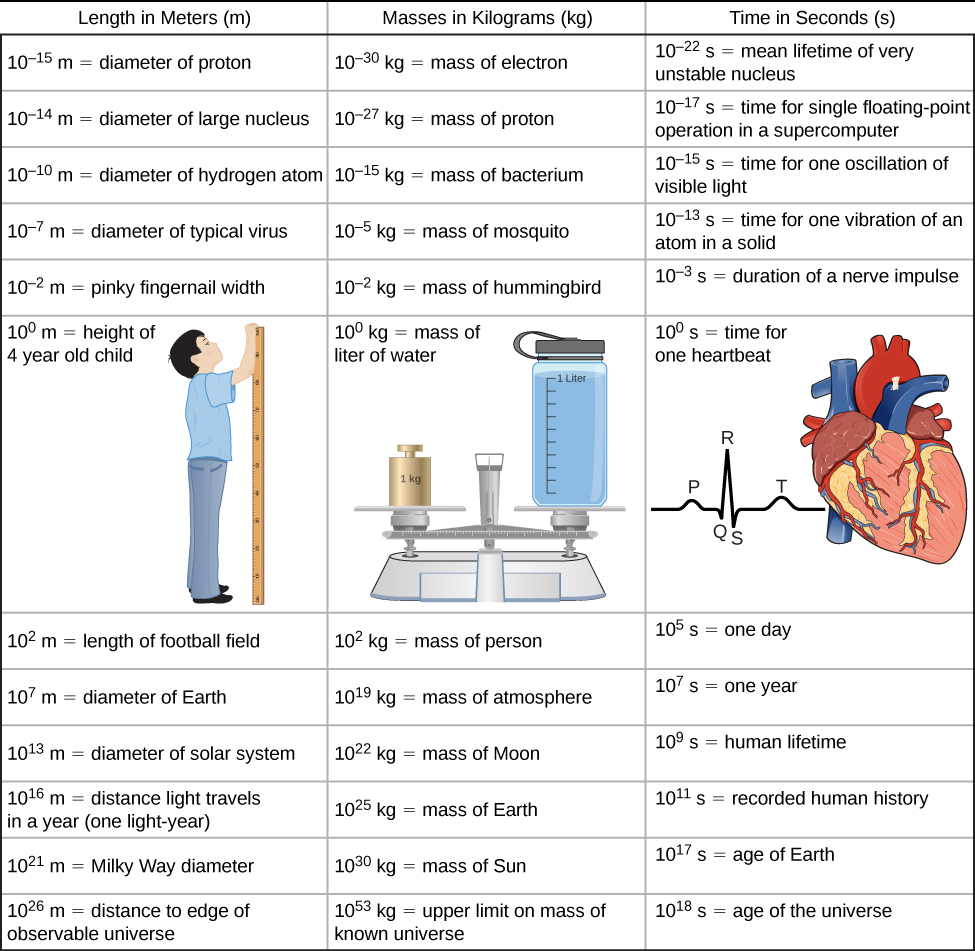
\includegraphics[scale=.7]{./figures/physfig1.jpeg  }
            \end{center}
        \item \textbf{SI Units: Base and Derived Units}}:
            \bigbreak \noindent 
            \begin{tabularx}{\textwidth}{|X|X|}
                \hline
                ISQ Base Quantity & SI Base Unit \\
                \hline
                Length & meter (m) \\
                Mass & kilogram (kg) \\
                Time & second (s) \\
                Electrical current & ampere (A) \\
                Thermodynamic temperature & kelvin (K) \\
                Amount of substance & mole (mol) \\
                Luminous intensity & candela (cd) \\
                \hline
            \end{tabularx}
            \pagebreak 
        \item \textbf{Metric Prefixes}}:
            \begin{center}
                \begin{tabularx}{\textwidth}{|X|X|X|X|X|X|}
                    \hline
                    Prefix & Symbol & Meaning & Prefix & Symbol & Meaning \\ 
                    \hline
                    yotta- & Y & $10^{24}$ & yocto- & y & $10^{-24}$ \\
                    zetta- & Z & $10^{21}$ & zepto- & z & $10^{-21}$ \\
                    exa-   & E & $10^{18}$ & atto-  & a & $10^{-18}$ \\
                    peta-  & P & $10^{15}$ & femto- & f & $10^{-15}$ \\
                    tera-  & T & $10^{12}$ & pico-  & p & $10^{-12}$ \\
                    giga-  & G & $10^9$   & nano-  & n & $10^{-9}$  \\
                    mega-  & M & $10^6$   & micro- & $\mu$ & $10^{-6}$ \\
                    kilo-  & k & $10^3$   & milli- & m & $10^{-3}$ \\
                    hecto- & h & $10^2$   & centi- & c & $10^{-2}$ \\
                    deka-  & da & $10^1$  & deci-  & d & $10^{-1}$ \\
                    \hline
                \end{tabularx}
            \end{center}
            \bigbreak \noindent 
        \item \textbf{Base Quantity \& Symbol for Dimension}}:
            \begin{center}
                \begin{tabularx}{\textwidth}{|X|X|}
                    \hline
                    Base Quantity & Symbol for Dimension \\
                    \hline
                    Length & L \\
                    Mass & M \\
                    Time & T \\
                    Current & I \\
                    Thermodynamic temperature & $\Theta$ \\
                    Amount of substance & N \\
                    Luminous intensity & J \\
                    \hline
                \end{tabularx}
            \end{center}
    \end{itemize}

    \pagebreak 
    \subsubsection{Memorize conversions}
    \begin{itemize}
        \item \textbf{Newton to Pounds}}: 
            \begin{align*}
                1N = 0.225lbs
            .\end{align*}
        \item \textbf{Pounds to newtons}}:
            \begin{align*}
                1lb = 4.448\ N
            .\end{align*}
        \item \textbf{Length/Distance }}:
            \begin{itemize}
                \item 1 inch (in) = 2.54 centimeters (cm)
                \item 1 centimeter (cm) = 0.393701 inches (in)
                \item 1 foot (ft) = 0.3048 meters (m)
                \item 1 meter (m) = 3.28 feet (ft)
                \item 1 mile (mi) = 1.6 kilometers (km)
                \item 1 kilometer (km) = 0.621371 miles (mi)
            \end{itemize}
    \item \textbf{Weight to mass or mass to weight}}:
        \begin{itemize}
            \item 1 pound = 0.453592 kilograms.
            \item 1 kilogram = 2.2 pounds.
        \end{itemize}
    \end{itemize}



    \pagebreak 
    \subsubsection{Problems to remember}
    \begin{itemize}
        \item \textbf{Restating mass}: Restate the mass  $1.93 \times 10^{13}}:$ using a metric prefix such that the resulting numerical value is bigger than one but less than 1000.
            \bigbreak \noindent 
            First, we must restate in terms of grams. Since $1kg = 10^{3}g$, we write
            \begin{align*}
                &1.93 \times 10^{13} \times 10^{3}g \\
                &1.93 \times 10^{16}g
            .\end{align*}
            Since $1Pg = 10^{15}g$, we can write
            \begin{align*}
               1.93 \times 10^{1}Pg 
            .\end{align*}
            Since $16-15 = 1 $
        \item \textbf{Unit conversion}}: The distance from the university to home is 10 mi and it usually takes 20 min to drive this distance. Calculate the average speed in meters per second (m/s). (Note: Average speed is distance traveled divided by time of travel.)
        \bigbreak \noindent 
        \textbf{Note:} There are 1609 meters in 1 mile
        \bigbreak \noindent 
        First, we can compute the average speed with the units given $\left(\frac{miles}{minute}\right)$
        \begin{align*}
            \text{Average Speed} = \frac{\text{miles}}{\text{minute}} = \frac{10}{20} = 0.5\ mi/min
        .\end{align*}
        \bigbreak \noindent 
        Now we simply convert to m/s
        \begin{align*}
            &\frac{0.5\ \cancel{mi}}{1\ \cancel{min}} \times \frac{1\ \cancel{min}}{60\ sec} \times \frac{1609\ m}{1\ \cancel{mi}} \\
            &\approx 13 m/s
        .\end{align*}
    \item \textbf{Unit conversion}: The density of iron is  $7.86 g/cm^{3}$ under standard conditions. Convert this to $kg/m^{3}}:$.
        \begin{align*}
            &\frac{7.86\ g}{1\ cm^{3}} \times \left(\frac{100\ cm}{1\ m}\right)^{3} \times \frac{1\ kg}{1000\ g} \\
            &= \frac{7.86(100^{3})(1\ kg)}{1000(1\ m)} \\
            &=7.86 \cdot 10^{3} kg/m^{3}
        .\end{align*}
    \item \textbf{Proportional}}: I found that if I drive my car 110 miles, I use 4 gallons ofgas. If I assume that the relationship between gas guzzled and distance driven is linearly proportional, how many gallons of gas do I use if I drive 275 miles?
        \bigbreak \noindent 
        To answer this lets find the linear equation
        \begin{align*}
            4\ gal = k(100\ mi)
        .\end{align*}
        Where $k$ is some arbitrary factor, Since we know the relationship is proportional, we can write 
        \begin{align*}
            &\frac{X}{4 gal} = \frac{k(275\ mi)}{k(110\ mi)} \\
            &X=10\ gal
        .\end{align*}

    \end{itemize}

    \pagebreak 
    \subsection{Chapter 2: Vectors}

    \smallbreak \noindent
    \subsubsection{Vocabulary}
    \begin{itemize}
        \item \textbf{scalar quantities}}:.
        \item \textbf{vector quantities}}:. Examples of vector quantities include displacement, velocity, position, force, and torque.
    \end{itemize}

    \pagebreak 
    \subsubsection{Definitions and theorems (and important things)}
    \begin{itemize}
        \item \textbf{direction}}:
        \item \textbf{Algebraic Operations with vectors}}:
            \begin{itemize}
                \item \textbf{add or subtract}}: two vectors
                \item \textbf{multiply}}: a vector by a scalar or by another vector
                \item \textbf{cannot}}: divide by a vector. The operation of division by a vector is not defined.
            \end{itemize}
        \item \textbf{Vector Notation}}: We denote a vector with a bold face letter with an arrow above it. For example
            \begin{align*}
                \vec{\textbf{V}}
            .\end{align*}
        \item \textbf{Displacement}}: General term used to describe change in position.
        \item \textbf{The magnitude of a vector is the length of the arrow used to represent it}}:

        \item \textbf{Vector relations}}:
            \fig{.8}{./figures/vectorimage1.jpeg}

        \item \textbf{Scalars}: When a vector $\vec{A}$ is multiplied by a positive scalar $\alpha$, the result is a new vector $\vec{B}$ that is parallel to $\vec{A}}:$:
            \begin{align*}
                \vec{\textbf{B}} = \alpha \vec{\textbf{A}}
            .\end{align*}
            The magnitude of this new vector $\vec{\textbf{B}}$ is 
            \begin{align*}
                B = |\alpha|A
            .\end{align*}
            Where $B$ is the magnitude of $\vec{\textbf{B}} $ and $A$ is the magnitude of $\vec{\textbf{A}} $ 
        \item \textbf{B}}}:$ of equal magnitude. If there are antiparallel, we write
            \begin{align*}
                \vec{\textbf{A}} = -\vec{\textbf{B}} 
            .\end{align*}
        \item \textbf{resultant}}:
        \item \textbf{resultant}}:
        \item \textbf{Vector Laws }}:
            \begin{itemize}
                \item \textbf{Communitive law}: $\vec{A} + \vec{B} = \vec{B} + \vec{A}}:$
                \item \textbf{Assosiative law}: $(\vec{A} + \vec{B}) + \vec{C} = \vec{A} + (\vec{B} + \vec{C}}:)$ 
                \item \textbf{Distributive law}: $\alpha_1 \vec{A} + \alpha_2 \vec{A} = (\alpha_1 + \alpha_2)\vec{A}}:$
            \end{itemize}
        \item \textbf{Vector addition}}:
            \begin{align*}
               \vec{\textbf{A}} + \vec{\textbf{B}} 
            .\end{align*}
            When two vectors are parallel, we can simply sum their magnitudes. However, if the vectors lie in different directions, the approach for vector addition involves finding their $x$ and $y$ components, summing them and then finding the magnitude. 
        \item \textbf{Vector Subtraction}}:
            \begin{align*}
                \vec{\textbf{A}} + (-\vec{\textbf{B}})
            .\end{align*}
            \bigbreak \noindent 
            When two vectors are aligned but point in exactly opposite directions, you can subtract their magnitudes (assuming you define one direction as positive and the other as negative) to find the net effect. This is a specific case of adding magnitudes where the direction is implicitly considered through subtraction.
        \item \textbf{Unit Vector notation}}:  A unit vector in a normed vector space is a vector of length 1. We declare unit vectors with a hat instead of an arrow, consider the following example
            \begin{align*}
                \hat{\textbf{u}}
            .\end{align*}
            We usually denote the unit vector along the positive x-axis $\hat{i}$, the unit vector along the positive y-axis $\hat{j}$, and the unit vector along the positive z-axis $\hat{k}$
        \item \textbf{Unit vector example}: For example, instead of saying vector $\vec{D}_{AB}$ has a magnitude of $6.0\,\text{km}$ and a direction of northeast, we can introduce a unit vector $\hat{u}$ that points to the northeast and say succinctly that $\vec{D}_{AB} = (6.0\,\text{km})\hat{u}$. Then the southwesterly direction is simply given by the unit vector $-\hat{u}$. In this way, the displacement of $6.0\,\text{km}}:$ in the southwesterly direction is expressed by the vector
            \begin{align*}
                    \vec{D}_{BA} = (-6.0\,\text{km})\hat{u}.
            .\end{align*}
        \item \textbf{Parallelogram rule for resultant or difference vectors in two dimensions.}}:
            \bigbreak \noindent 
            \fig{.8}{./figures/res.jpeg}
            \bigbreak \noindent 
            It follows from the parallelogram rule that neither the magnitude of the resultant vector nor the magnitude of the difference vector can be expressed as a simple sum or difference of magnitudes A and B, because the length of a diagonal cannot be expressed as a simple sum of side lengths.
        \item \textbf{tail-to-head geometric construction}}:
            \bigbreak \noindent 
            \fig{.8}{./figures/res2.jpeg}
        \item \textbf{Vector $x$ and $y$ components}: The $x$ component can be denoted, $\vec{A_{x}}$ the $y$ component can be denoted $\vec{A_{y}}}:$. Thus, the vector can be represented as
            \begin{align*}
                &\vec{A} = \vec{A_{x}} + \vec{A_{y}}
            .\end{align*}
        \item \textbf{Unit vectors of the axes}:     It is customary to denote the positive direction on the $x$-axis by the unit vector $\hat{i}$ and the positive direction on the $y$-axis by the unit vector $\hat{j}$. Unit vectors of the axes, $\hat{i}$ and $\hat{j}}:$, define two orthogonal directions in the plane. The $x$- and $y$- components of a vector can now be written in terms of the unit vectors of the axes:
            \bigbreak \noindent 
               \begin{equation}
                    \begin{cases}
                        \vec{A}_{x} &= A_{x}\hat{i}  \\
                         \vec{A}_{y} &= A_{y}\hat{j}  
                    \end{cases}
                \end{equation}
        \item \textbf{Component form of a vector}}:
            \begin{align*}
                \vec{A} = A_{x}\hat{i} + A_{y}\hat{j}
            .\end{align*}
        \item \textbf{Finding components given initial and terminal points}}: If we know the coordinates $b(x_b, y_b)$ of the origin point of a vector (where $b$ stands for "beginning") and the coordinates $e(x_e, y_e)$ of the end point of a vector (where $e$ stands for "end"), we can obtain the scalar components of a vector simply by subtracting the origin point coordinates from the end point coordinates:
            \begin{align*}
                A_x &= x_e - x_b  \\
                A_y &= y_e - y_b
            .\end{align*}
        \item \textbf{Magnitude $A$ of a vector with components $A_{x}$ and $A_{y}$}}:
            \begin{align*}
               &A^{2}  = A_{x}^{2} + A_{y}^{2} \\
               &A = \sqrt{A_{x}^{2} + A_{y}^{2}}
            .\end{align*}
            This equation works even if the scalar components of a vector are negative.
        \item \textbf{Finding theta for a vector (used for direction angles)}}:
            \begin{align*}
                \tan{\theta } = \frac{A_{y}}{A_{x}}
            .\end{align*}
        \item \textbf{Direction angles for vectors in the first}}:
        \item \textbf{Direction angles for vectors in the second quadrant}}:
            \begin{align*}
                \theta_{A} = \theta 
            .\end{align*}
        \item \textbf{Direction angles for vectors in the second quadrant}}:
            \begin{align*}
                \theta_{A} = 180 - \theta 
            .\end{align*}
        \item \textbf{Direction angles for vectors in the second quadrant}}:
            \begin{align*}
                \theta_{A} = 180 + \theta 
            .\end{align*}
        \item \textbf{Direction angles for vectors in the fourth quadrant}}:
            \begin{align*}
                \theta_{A} = 360 - \theta 
            .\end{align*}
        \item \textbf{Finding $A_{x}$ and $A_{y}$  when the magnitude and direction angle are known}}:
        \begin{equation}
            \begin{cases}
                &A_{x} = A\cos{\theta_{A}} \\
                &A_{y} = A\sin{\theta_{A}} \\
            \end{cases}
        \end{equation}
        \item \textbf{Polar form}}:
            \begin{align*}
                &x = r\cos{\varphi} \\
                &y = r\sin{\varphi}
            .\end{align*}
        \item \textbf{Three dimensional plane}}:
            \bigbreak \noindent 
            \fig{.8}{./figures/zaxis.jpeg}
        \item \textbf{$z$ component of a vector}}:
            \begin{align*}
                \vec{A}_{z} = A_{z}\hat{k} 
            .\end{align*}
            Where $A_{z}$ is given by 
            \begin{align*}
                z_{e} - z_{b}
            .\end{align*}
        \item \textbf{Vector in three dimensions}}: A vector in three-dimensional space is the vector sum of its three vector component. 
            \begin{align*}
                \vec{A} = A_x \hat{i} + A_y \hat{j} + A_z \hat{k}.
            .\end{align*}
        \item \textbf{Magnitude of a vector in three dimensions}}:
            \begin{align*}
                A = \sqrt{A_x^2 + A_y^2 + A_z^2}.
            .\end{align*}
        \item \textbf{Null vector}}: Denoted by 
            \begin{align*}
                \vec{0}
            .\end{align*}
            Has all components 0. Thus, 
            \begin{align*}
                \vec{0} = 0\hat{i} + 0\hat{j} + 0\hat{k}
            .\end{align*}
            Thus, it has no direction and no length
        \item \textbf{equal vectors}}: if and only if their difference is the null vector:
        Hence, we can write $\vec{A} = \vec{B}$ if and only if the corresponding components of vectors $\vec{A}$ and $\vec{B}$ are equal:
        \[
        \vec{A} = \vec{B} \Leftrightarrow
        \left\{
            \begin{array}{l}
                A_x = B_x \\
                A_y = B_y \\
                A_z = B_z
            \end{array}
        \right.
        \]
    \item \textbf{Components of a resultant vector}}:
        \begin{equation}
            \begin{cases}
                R_{x} = A_{x}  + B_{x} \\
                R_{y} = A_{y}  + B_{y} \\
                R_{z} = A_{z}  + B_{z} 
            \end{cases}
        \end{equation}

    \item \textbf{components of a resultant of many vectors}: if we are to sum up $N$ vectors $\vec{F}_1, \vec{F}_2, \vec{F}_3, \ldots, \vec{F}_N$, where each vector is $\vec{F}_k = F_{kx}\hat{i} + F_{ky}\hat{j} + F_{kz}\hat{k}$, the resultant vector $\vec{F}}:_R$ is
           \begin{equation}
                \begin{cases}
                    F_{R_{x}} = \summation{N}{k=1}\ F_{kx}\ = F_{1x} + F_{2x} + F_{3x} + ... + F_{Nx} \\
                    F_{R_{y}} = \summation{N}{k=1}\ F_{ky}\ = F_{1y} + F_{2y} + F_{3y} + ... + F_{Ny} \\
                    F_{R_{z}} = \summation{N}{k=1}\ F_{kz}\ = F_{1z} + F_{2z} + F_{3z} + ... + F_{Nz} \\
                \end{cases}
            \end{equation}
        With the component form 
        \begin{align*}
            \vec{F_{R}} = F_{R_{x}}\hat{i} + F_{R_{y}}\hat{j} + F_{R_{z}}\hat{k}
        .\end{align*}
    \item \textbf{Finding unit vector (Direction) of some vector}: Suppose we have some vector $\vec{V}}:$. Then 
        \begin{align*}
            \hat{V} = \frac{\vec{V}}{V}
        .\end{align*}
    \item \textbf{Dot product}}:
        \begin{align*}
            \vec{A} \cdot \vec{B} = AB\cos{\varphi} 
        .\end{align*}
        Where $\varphi$ is the angle between the vectors
    \item \textbf{Dot product of two parallel vectors}}:
        \begin{align*}
            \vec{A} \cdot \vec{B} = AB\cos{0^{\circ}} = AB
        .\end{align*}
    \item \textbf{Dot product of two anti-parallel vectors}}:
        \begin{align*}
            \vec{A} \cdot \vec{B} = AB\cos{180^{\circ}} = -AB
        .\end{align*}
    \item \textbf{Dot product of two orthogonal vectors}}:
        \begin{align*}
            \vec{A} \cdot \vec{B} = AB\cos{90^{\circ}} =  0
        .\end{align*}
    \item \textbf{Dot product of a vector with itself}}:
        \begin{align*}
            \vec{A} \cdot \vec{A} = AA\cos{0} = A^{2}
        .\end{align*}
    \item \textbf{Dot products of unit vectors}}: Scalar products of the unit vector of an axis with other unit vectors of axes always vanish (equals 0) because these unit vectors are orthogonal:
    \item \textbf{Dot product of the same unit vector}}: The dot product of the same unit vector is 1
        \begin{align*}
            \hat{i} \cdot \hat{i} = i^{2} = 1
        .\end{align*}
    \item \textbf{Using dot product to find scalar x-component}}:
        \begin{align*}
            \vec{A} \cdot \hat{i} = \norm{\vec{A}} \norm{\hat{i}}\cos{\theta_{A}} = A\cos{\theta_{A}}= A_{x}
        .\end{align*}
    \item \textbf{Using dot product to find scalar y-component}}:
        \begin{align*}
            \vec{A} \cdot \hat{j} = \norm{\vec{A}} \norm{\hat{j}}\cos{(90^{\circ} -\theta_{A})}= A\sin{\theta_{A}} = A_{y}
        .\end{align*}
    \item \textbf{Trig complementary angles}}: For a right angle triangle, the sine of the complemenary angle is the cosine of the angle. And vice versa
        \begin{align*}
            &\sin{90-\theta} = \cos{\theta} \\
            &\cos{90-\theta} = \sin{\theta}
        .\end{align*}
    \item \textbf{Dot product second method of computation}}:
        \begin{align*}
            \vec{A} \cdot \vec{B} = A_{x}B_{x} + A_{y}B_{y} + A_{z}B_{z}
        .\end{align*}
    \item \textbf{Equation for $\cos{(\varphi)}$}}:
        \begin{align*}
            \cos{(\varphi)} = \frac{\vec{A} \cdot \vec{B}}{AB}
        .\end{align*}
    \item \textbf{Si unit for work}}: is the joule (J), where 
        \begin{align*}
            1\ \text{J} = 1\ \text{N} \cdot \text{m} 
        .\end{align*}
    \item \textbf{The Work of a Force}: When force $\vec{F}$ pulls on an object and when it causes its displacement $\vec{D}$, we say the force performs work. The amount of work the force does is the scalar product $\vec{F} \cdot \vec{D}}:$.
    \item \textbf{Cross Product (Vector Product)}}: 
        The vector product of two vectors $\vec{A}$ and $\vec{B}$ is denoted by $\vec{A} \times \vec{B}$ and is often referred to as a cross product. The vector product is a vector that has its direction perpendicular to both vectors $\vec{A}$ and $\vec{B}$. In other words, vector $\vec{A} \times \vec{B}$ is perpendicular to the plane that contains vectors $\vec{A}$ and $\vec{B}$. The magnitude of the vector product is defined as
        \begin{equation}
            \lVert \vec{A} \times \vec{B} \rVert = AB \sin \varphi,
        \end{equation}
        where angle $\varphi$, between the two vectors, is measured from vector $\vec{A}$ (first vector in the product) to vector $\vec{B}$ (second vector in the product), as indicated in Figure 2.29, and is between $0^\circ$ and $180^\circ$.
    \item \textbf{antiparallel}}: ($\varphi=180^\circ$) because $\sin 0^\circ = \sin 180^\circ = 0$.
    \item \textbf{anti-communitive}}:
        \begin{align*}
            \vec{A} \times \vec{B} = -\vec{B} \times \vec{A}.
        .\end{align*}
    \item \textbf{Torque}}: Denoted with the greek letter "tau" is the vector product of the distance between the pivot to force with the force:
        \begin{align*}
            \vec{\tau} = \vec{R} \times \vec{F}
        .\end{align*}
    \item \textbf{the cross product has the following distributive property:}}:
        \begin{align*}
            \vec{A} \times (\vec{B} + \vec{C}) = \vec{A} \times \vec{B} + \vec{A} \times \vec{C}
        .\end{align*}
    \item \textbf{Cross product of the same unit vectors}}: The cross product of the same unit vectors is 0
    \item \textbf{Cross product between unit vectors}}:
        \begin{equation}
            \begin{cases}
                \hat{i} \times \hat{j} = +\hat{k} \\
                \hat{j} \times \hat{i} = -\hat{k} \\
                \hat{j} \times \hat{k} = +\hat{i} \\
                \hat{k} \times \hat{j} = -\hat{i} \\
                \hat{k} \times \hat{i} = +\hat{j} \\
                \hat{i} \times \hat{k} = -\hat{j}
            \end{cases}
        \end{equation}
        \bigbreak \noindent 
        \textbf{Notice:} The cross product of two different unit vectors is always a third unit vector.
    \item \textbf{Computation of the cross product}}:
        \begin{align*}
            \vec{C} = \vec{A} \times \vec{B} = (A_yB_z - A_zB_y)\hat{i} + (A_zB_x - A_xB_z)\hat{j} + (A_xB_y - A_yB_x)\hat{k}
        .\end{align*}
        \pagebreak 
    \item \textbf{vector quantity}}: of speed plus the direction. Velocity is 
        \begin{align*}
            \vec{v} &=\frac{\text{Displacement}}{Time} = \frac{\norm{\vec{d}}}{t}
        .\end{align*}
        Where $\norm{\vec{d}}$ is the magnitude of the displacement vector, and $t$ is the total elapsed time.
    \item \textbf{position vector}}:, Denoted
        \begin{align*}
            \vec{r}
        .\end{align*}
        \bigbreak \noindent 
    \begin{figure}[ht]
        \centering
        \incfig{try2}
        \label{fig:try2}
    \end{figure}
    \item \textbf{Displacement}}: is defined as the change in the position vector. The final position vector minus the initial position vector
        \begin{align*}
            \Delta \vec{r} = \vec{r}_{f} - \vec{r}_{i}
        .\end{align*}
    \begin{figure}[ht]
        \centering
        \incfig{hellowrold}
        \label{fig:hellowrold}
    \end{figure}






    \end{itemize}

    \pagebreak 
    \subsubsection{Problems to remember}
    \begin{itemize}
        \item \textbf{Unit vectors}}: A long measuring stick rests against a wall in a physics laboratory with its 200-cm end at the floor. A ladybug lands on the 100-cm mark and crawls randomly along the stick. It first walks 15 cm toward the floor, then it walks 56 cm toward the wall, then it walks 3 cm toward the floor again. Then, after a brief stop, it continues for 25 cm toward the floor and then, again, it crawls up 19 cm toward the wall before coming to a complete rest (Figure 2.8). Find the vector of its total displacement and its final resting position on the stick.
        \bigbreak \noindent 
        If we choose the direction along the stick toward the floor as the direction of unit vector $\hat{u}$, then the direction toward the floor is $+\hat{u}$ and the direction toward the wall is $-\hat{u}$. The ladybug makes a total of five displacements:
    \begin{align*}
        &\vec{D}_1 = (15\,\text{cm})(+\hat{u}), \quad \vec{D}_2  \\
        &= (56\,\text{cm})(-\hat{u}), \quad \vec{D}_3  \\
        &= (3\,\text{cm})(+\hat{u}), \quad \vec{D}_4  \\
        &= (25\,\text{cm})(+\hat{u}), \quad \text{and} \quad \vec{D}_5  \\
        &= (19\,\text{cm})(-\hat{u}).
    .\end{align*}
    The total displacement $\vec{D}$ is the resultant of all its displacement vectors.
    \bigbreak \noindent 
    The resultant of all the displacement vectors is
    \begin{align*}
        &\vec{D} = \vec{D}_1 + \vec{D}_2 + \vec{D}_3 + \vec{D}_4 + \vec{D}_5  \\
        &= (15\,\text{cm})(+\hat{u}) + (56\,\text{cm})(-\hat{u}) + (3\,\text{cm})(+\hat{u}) + (25\,\text{cm})(+\hat{u}) + (19\,\text{cm})(-\hat{u})  \\
        &= (15 - 56 + 3 + 25 - 19)\,\text{cm}\,\hat{u} = -32\,\text{cm}\,\hat{u}
    .\end{align*}
    In this calculation, we use the distributive law. The result reads that the total displacement vector points away from the 100-cm mark (initial landing site) toward the end of the meter stick that touches the wall. The end that touches the wall is marked 0 cm, so the final position of the ladybug is at the $(100 - 32)\,\text{cm} = 68\,\text{cm}$ mark.
    \end{itemize}

    \pagebreak 
    \subsection{Chapter 3: Motion along a straight line}
    \bigbreak \noindent 
    \subsubsection{Definitions and theorems}
    \begin{itemize}
        \item \textbf{Kinematics}}: is a subfield of physics, developed in classical mechanics, that describes the motion of points, bodies, and systems of bodies without considering the forces that cause them to move
        \item \textbf{Displacement}}: Displacement $\Delta x$ is the change in position of an object:
            \begin{align*}
                \Delta x = x_f - x_0,
            .\end{align*}
            where $\Delta x$ is displacement, $x_f$ is the final position, and $x_0$ is the initial position.
        \item We define total displacement $\Delta x_{\text{Total}}$, as the sum of the individual displacements, and express this mathematically with the equation
            \begin{align*}
                \Delta x_{\text{Total}} = \sum \Delta x_i
            .\end{align*}
        \item \textbf{the distance traveled}}: is the sum of the magnitudes of the individual displacements:
            \begin{align*}
                x_{\text{total}} = \summation{n}{i=1}\ \Delta x_{i}
            .\end{align*}
        \item \textbf{average velocity}. If  $x_{1}$ and  $x_{2} $ are the positions of an object at times  $t_{1} $ and  $t_{2}}:$ , respectively, then 
            \begin{align*}
                \text{Average Velocity } =\ &\bar{v} =  \frac{\text{Displacement between two points}}{\text{Time needed to make the displacement}} \\
                &\bar{v} = \frac{\Delta x}{\Delta t} = \frac{x_{2} - x_{1}}{t_{2} - t_{1}}
            .\end{align*}
        
            This vector quantity is simply the total displacement between two points divided by the time taken to travel between them. The time taken to travel between two points is called the \textbf{elapsed time} $\Delta t$
        \item \textbf{instantaneous velocity}}: of an object is the limit of the average velocity as the elapsed time approaches zero, or the derivative of $x$ with respect to $t$:
            \begin{align*}
                v(t) &= \lim\limits_{\Delta t \to 0}{\frac{f(t + \Delta t) - f(t)}{\Delta t}} \\
                 &= \frac{d}{dt}x(t) = \frac{d\vec{r}}{dt}.
            .\end{align*}
        \item \textbf{average speed}}: by finding the total distance traveled divided by the elapsed time:
            \begin{align*}
                \text{Average speed } = \bar{s} = \frac{\text{Total distance}}{\text{Elapsed time}}.
            .\end{align*}
        \item \textbf{instantaneous speed}}: from the magnitude of the instantaneous velocity:
            \begin{align*}
                \text{instantaneous speed } = \bigg\lvert v(t) \bigg\rvert
            .\end{align*}
        \item \textbf{Calculating Instantaneous Velocity}}:
            When calculating instantaneous velocity, we need to specify the explicit form of the position function $x(t)$. If each term in the $x(t)$ equation has the form of $A t^n$ where $A$ is a constant and $n$ is an integer, this can be differentiated using the power rule to be:
            \begin{align*}
                \frac{d(At^{n})}{dt}= Ant^{n-1}
            .\end{align*}
        \item \textbf{Average acceleration}}: is the rate at which velocity changes:
            \begin{align*}
                \bar{a} = \frac{\Delta v}{\Delta t} = \frac{v_f - v_0}{t_f - t_0},
            .\end{align*}
            where $\bar{a}$ is average acceleration, $v$ is velocity, and $t$ is time. (The bar over the $a$ means average acceleration.)
            \bigbreak \noindent 
            \textbf{Note:} acceleration occurs when velocity changes in magnitude (an increase or decrease in speed) or in direction, or both.
               \item \textbf{Acceleration as a vector:}}: Acceleration is a vector in the same direction as the change in velocity,  $\Delta v$ . Since velocity is a vector, it can change in magnitude or in direction, or both. Acceleration is, therefore, a change in speed or direction, or both.
         \bigbreak \noindent 
         Keep in mind that although acceleration is in the direction of the change in velocity, it is not always in the direction of motion. When an object slows down, its acceleration is opposite to the direction of its motion. Although this is commonly referred to as deceleration
        \item \textbf{Distance over constant acceleration}}:
            \begin{align*}
                d = \frac{1}{2}at^{2} 
            .\end{align*}
            Where $a$ is the acceleration, and $t$ is the time
        \item \textbf{instantaneous acceleration}}:
            \begin{align*}
            a(t) = \frac{d}{dt}v(t)
            .\end{align*}
        \item \textbf{Derivative of velocity function}}: Suppose we have some function 
            \begin{align*}
                v(t) = (20 m/s) t - (10 m/s^{2})t^{2}
            .\end{align*}
            When we find the acceleration function, we are taking the derivative of the velocity function. Thus, we are finding the change in velocity with respect to time. Consequently, our terms become
            \begin{align*}
                a(t) = 20 m/s^{2} - (10m/s^{3})t
            .\end{align*}
            \textbf{Notice:} How we are dividing by an additional unit of time, thus the exponents for our seconds increases by one.
        \item \textbf{Simplified notation}}: If we take initial time to be zero, and final quantitys without subscript, then we have 
            \begin{align*}
               &\Delta t = t\\
                &\Delta x = x - x_{0}\\
                &\Delta v = v- v_{0}\\
            .\end{align*}
        \item \textbf{Assumption of constant acceleration}}: This assumption allows us to avoid using calculus to find instantaneous acceleration. Since acceleration is constant, the average and instantaneous accelerations are equal—that is,
            \begin{align*}
                \bar{a} = a = \text{constant}
            .\end{align*}
            Thus, we can use the symbol $a$ for acceleration at all times.
        \item \textbf{Final Position function}}: 
            \begin{align*}
                x = x_{0}  + \bar{v}t
            .\end{align*}
        \item \textbf{Average velocity under constant acceleration}}:
            \begin{align*}
                \bar{v} = \frac{v_{0} + v}{2} \quad \text{(Constant $a$)}
            .\end{align*}
            This reflects the fact that when acceleration is constant, $\bar{v}$ is just the simple average of the initial and final velocities.
        \item \textbf{Final Velocity function under constant acceleration}}:
            \begin{align*}
                v = v_{0} + at \quad \text{(Constant $a$)}
            .\end{align*}
        \item \textbf{Equation for final position under constant acceleration}}:
            \begin{align*}
                x = x_{0} +v_{0}t + \frac{1}{2}at^{2} \quad \text{(Constant $a$)}
            .\end{align*}
            When initial position and velocity are both zero, we have
            \begin{align*}
                x =  \frac{1}{2}at^{2} \quad \text{(Constant $a$)}
            .\end{align*}
        \item \textbf{relationships seen in final position under constant acceleration equation}}:
            \begin{itemize}
                \item Displacement depends on the square of the elapsed time when acceleration is not zero.
                \item If acceleration is zero, then initial velocity equals average velocity \(v_0 = \bar{v}\), and \(x = x_0 + v_0t + \frac{1}{2}at^2\) becomes \(x = x_0 + v_0t\).
            \end{itemize}
        \item \textbf{Final velocity equation (no time required)}}:
            \begin{align*}
                v^{2} = v_{0}^{2} + 2a(x-x_{0}) \quad \text{(Constant $a$)}
            .\end{align*}
        \item \textbf{additional insights into the general relationships among physical quantities:}}:
            \begin{itemize}
                \item The final velocity depends on how large the acceleration is and the distance over which it acts.
                \item For a fixed acceleration, a car that is going twice as fast doesn’t simply stop in twice the distance. It takes much farther to stop. (This is why we have reduced speed zones near schools.)
            \end{itemize}
        \item \textbf{acceleration in terms of velocities and displacement}}:
            \begin{align*}
                a  = \frac{v^{2} - v_{0}^{2}}{2(x-x_{0})}
            .\end{align*}
        \item \textbf{two-body pursuit problems}}:
            \begin{itemize}
                \item Find equations of motion for both bodies (with the same parameter)
                \item eliminate the parameter
                \item plug in knowns to solve for the unknown
            \end{itemize}
        \item \textbf{constant acceleration, independent of their mass.}}: 
        \item \textbf{free fall}}:
        \item \textbf{acceleration due to gravity}}:
            \begin{align*}
                g = 9.8\ m/s^{2}
            .\end{align*}
            \textbf{Note:} If we define the upward direction as positive, then   $a=−g=-9.8m/s^{2},$ and if we define the downward direction as positive, then  $a=g=9.8m/s^{2}$
        \item \textbf{vertical displacement}}: We denote vertical displacement with the symbol $y$
        \item \textbf{Kinematic equations for objects in free fall}}: We assume here that acceleration equals -g (with the positive direction upward).
            \begin{align*}
                v &= v_{0} - gt \\
                y &= y_{0} + v_{0}t-\frac{1}{2}gt^{2} \\
                v^{2} &= v_{0}^{2} -2g(y-y_{0})
            .\end{align*}
        \item \textbf{Change in velocity}}:
            \begin{align*}
                \Delta v = a\Delta t
            .\end{align*}
            If you don't care about position this relates the acceleration,  intervals of time and changes in velocity
        \item \textbf{Change in position}}:
            \begin{align*}
                \Delta x = \frac{1}{2}(v_{f} - v_{i})\Delta t
            .\end{align*}
    \end{itemize}

    \pagebreak 
    \subsection{Chapter 4: Motion in two and three dimensions}
    \smallbreak \noindent
    \subsubsection{Definitions and theorems}
    \begin{itemize}
        \item \textbf{Location of a particle in space}}:
            \begin{align*}
                x &= x(t) \\
                y &= y(t) \\
                z &= z(t)
            .\end{align*}
            Where $x,y,z$ are functions of time ($t$). 
        \item \textbf{Position vector in space}}:
            \begin{align*}
                \vec{\mathbf{r}}(t) = x(t)\hat{\mathbf{i}} + y(t)\hat{\mathbf{j}} + z(t)\hat{\mathbf{k}}
            .\end{align*}
        \item \textbf{Displacement vector in space}}: 
            Suppose we have a particle. At time $t_{1}$ the particle is located at $P_{1}$ with position vector $\vec{\mathbf{r}}(t_{1})$. At some later time $t_{2}$, the particle is located at $P_{2}$ with position vector $\vec{\mathbf{r}}(t_{2})$. The displacement vector $\vec{\Delta r}$ is found by subtracting $\vec{r}(t_1)$ from $\vec{r}(t_2)$:
            \begin{align*}
                \Delta \vec{\mathbf{r}} = \vec{\mathbf{r}}(t_{2}) - \vec{\mathbf{r}}(t_{1})
            .\end{align*}
            Thus, the displacement vector $\Delta \vec{\mathbf{r}} = \vec{\mathbf{r}}(t_{2}) - \vec{\mathbf{r}}(t_{1})$ is the vector from $P_{1}$ to $P_{2}$
        \item \textbf{Instantaneous velocity vector in two and three dimensions}}: We can do the same operation in two and three dimensions, but we use vectors. The instantaneous velocity vector is now
            \begin{align*}
                \vec{\mathbf{v}} &= \lim\limits_{\Delta t \to 0}{\frac{\vec{\mathbf{r}}(t - \Delta t)-\vec{\mathbf{r}}(t)}{\Delta t}} \\
                &=\frac{d\vec{\mathbf{r}}}{dt}
            .\end{align*}
        \item \textbf{Velocity in component form}}:
            \begin{align*}
                \vec{\mathbf{v}}(t) = v_{x}\hat{\mathbf{i}} + v_{y}\hat{\mathbf{j}} + v_{z}\hat{\mathbf{k}}
            .\end{align*}
            Where 
            \begin{align*}
                v_{x}(t) = \frac{dx(t)}{dt}, \quad v_{y}(t) = \frac{dy(t)}{dt}, \quad v_{z}(t) = \frac{dz(t)}{dt}
            .\end{align*}
        \item \textbf{Average velocity in two and three dimensions}}: 
            If only the average velocity is of concern, we have the vector equivalent of the one-dimensional average velocity for two and three dimensions
            \begin{align*}
                \vec{\mathbf{v}}_{\text{avg}} = \frac{\vec{\mathbf{r}}(t_{2})-\vec{\mathbf{r}}(t_{1})}{t_{2} - t_{1}}
            .\end{align*}
        \item \textbf{The Independence of Perpendicular Motions}}: When we look at the three-dimensional equations for position and velocity written in unit vector notation, we see the components of these equations are separate and unique functions of time that do not depend on one another. Motion along the x direction has no part of its motion along the y and z directions, and similarly for the other two coordinate axes. Thus, the motion of an object in two or three dimensions can be divided into separate, independent motions along the perpendicular axes of the coordinate system in which the motion takes place.
        \item \textbf{Independence of motion}}: In the kinematic description of motion, we are able to treat the horizontal and vertical components of motion separately. In many cases, motion in the horizontal direction does not affect motion in the vertical direction, and vice versa.
        \item \textbf{Instantaneous Acceleration}: This acceleration vector is the instantaneous acceleration and it can be obtained from the derivative with respect to time of the velocity function. The only difference in two or three dimensions is that these are now vector quantities. Taking the derivative with respect to time $\vec{\mathbf{v}}}:(t) $. We find
            \begin{align*}
               \vec{\mathbf{a}}(t) = \frac{d\vec{\mathbf{v}}(t)}{dt} 
            .\end{align*}
        \item \textbf{The acceleration in terms of components is}}:
            \begin{align*}
                \vec{\mathbf{a}}(t) = \frac{dv_{x}(t)}{dt}\hat{\mathbf{i}} + \frac{dv_{y}(t)}{dt}\hat{\mathbf{j}} + \frac{dv_{z}(t)}{dt}\hat{\mathbf{k}}
            .\end{align*}
        \item \textbf{acceleration in terms of the second derivative of the position function:}}:
            \begin{align*}
                \vec{\mathbf{a}}(t) = \frac{d^{2}x(t)}{dt^{2}}\hat{\mathbf{i}} + \frac{d^{2}y(t)}{dt^{2}}\hat{\mathbf{j}} + \frac{d^{2}z(t)}{dt^{2}}\hat{\mathbf{k}}
            .\end{align*}
        \item \textbf{Equations for position and velocity in the two and three dimensions (8)}}:. For simplicity I will only list the ones for the x-direction. However, keep in mind that these same equations hold for $y$ and $z$
            \begin{itemize}
                \item \textbf{Position with initial position and average velocity:}}: 
                    \begin{align*}
                        x(t)&=x_0+\left(v_x\right)_{\text {avg }} t
                    .\end{align*}
                \item \textbf{Final velocity with initial velocity, acceleration, and time}}:
                    \begin{align*}
                        v_x(t)&=v_{0 x}+a_x t
                    .\end{align*}
                \item \textbf{Position}}:
                    \begin{align*}
                        x(t)&=x_0+v_{0 x} t+\frac{1}{2} a_x t^2
                    .\end{align*}
                \item \textbf{Velocity with initial velocity, acceleration, final and initial position}}:
                    \begin{align*}
                        v_x^2(t)&=v_{0 x}^2+2 a_x\left(x-x_0\right) 
                    .\end{align*}
            \end{itemize}
        \item \textbf{These equations can be substituted into the equations for the position and velocity vectors in component form, and velocity vector in component form without the z-component to obtain the position vector and velocity vector as a function of time in two dimensions:}}:
            \begin{align*}
                \vec{\mathbf{r}}(t) &= x(t)\hat{\mathbf{i}} + y(t)\hat{\mathbf{j}}\\
                \vec{\mathbf{v}}(t)&= v_{x}(t)\hat{\mathbf{i}} + v_{y}(t)\hat{\mathbf{j}}
            .\end{align*}
        \item \textbf{trajectory}}:
        \item \textbf{Acceleration in projectile motion}}: Defining the positive direction to be upward, the components of acceleration are then very simple:
            \begin{align*}
                a_{y} &= -9.8\ m/s^{2} \\
                a_{x} &= 0
            .\end{align*}
             Because gravity is vertical, $a_{x} = 0$. If  $a_{x} = 0$, this means the initial velocity in the $x$ direction is equal to the final velocity in the $x$ direction, or  $v_{x} = v_{0x} $
            \item \textbf{Kinematic equations for motion in a uniform gravitational field}}:
                \begin{itemize}
                    \item Horizontal motion 
                        \begin{align*}
                            v_{0x} = v_{x}, \quad x = x_{0} +v_{x}t
                        .\end{align*}
                    \item \textbf{Average velocity (vertical)}}:
                    \item Basic average velocity 
                        \begin{align*}
                            V_{y,\text{avg}} = \frac{y-y_{0}}{\Delta t}
                        .\end{align*}
                    \item \textbf{Average velocity in special conditions}}:
                        \begin{align*}
                            V_{y,\text{avg}} = \frac{v_i +v_f}{2}
                        .\end{align*}
                        \textbf{Note:} gives the same result for average velocity in scenarios of uniform acceleration, such as projectile motion or free fall, under specific conditions. This formula calculates the average of the initial and final velocities, assuming that the acceleration is constant throughout the motion. It works perfectly for the vertical component of projectile motion when considering the ascent or descent separately, or any motion where the start and end points are symmetrical in terms of velocity but in opposite directions (e.g., going up and coming back down to the same height).
                    \item Vertical motion
                        \begin{align*}
                            y &= y_{0} + \frac{1}{2}(v_{0y} + v_{y})t \\
                            v_{y}&= v_{0y} + gt \\
                            y &=y_{0}+v_{0y}t + \frac{1}{2}gt^{2} \\
                            v^{2}_{y} &= v_{0y}^{2}+2g(y-y_{0})
                        .\end{align*}
                \end{itemize}
            \item \textbf{Projectile motion max height}}:
                \begin{align*}
                    h = \frac{v_{0y}^{2}}{2g}
                .\end{align*}
                This equation defines the maximum height of a projectile above its launch position and it depends only on the vertical component of the initial velocity.
            \item \textbf{Parabolic trajectory}: If the motion is parabolic, we should use the equation with $t^{2}}:$ to solve for $t$ and vertical displacement
            \item \textbf{Time of flight}}: We can solve for the time of flight of a projectile that is both launched and impacts on a flat horizontal surface by performing some manipulations of the kinematic equations. We note the position and displacement in y must be zero at launch and at impact on an even surface. Thus, We set the displacement in y equal to zero and find
                \begin{align*}
                    T_{\text{tof}} = \frac{2(v_{0}\sin{\theta_{0}})}{g}
                .\end{align*}
                \textbf{Note:} This is the time of flight for a projectile both launched and impacting on a flat horizontal surface. This equation does not apply when the projectile lands at a different elevation than it was launched,
            \item \textbf{Trajectory}: The trajectory of a projectile can be found by eliminating the time variable $t$ from the kinematic equations for arbitrary $t$ and solving for $y(x)$. We take $x_{0} = y_{0}}: = 0$ so the projectile is launched from the origin. 
                \begin{align*}
                    y = (\tan{\theta_{0}})x - \left[\frac{g}{2(v_{0}\cos{\theta_{0}})^{2}}\right]x^{2}
                .\end{align*}
                \textbf{Note:} This trajectory equation is of the form $y=ax+bx^{2}$
                which is an equation of a parabola with coefficients
                \begin{align*}
                    a = \tan{\theta_{0}}, \quad b = -\frac{g}{2(v_{0}\cos{\theta_{0}})^{2}}
                .\end{align*}
            \item \textbf{Range}}: From the trajectory equation we can also find the range, or the horizontal distance traveled by the projectile.
                \begin{align*}
                    R = \frac{v_{0}^{2}\sin{(2\theta_{0})}}{g}
                .\end{align*}

            \item \textbf{time of flight, trajectory, and range}}:) are derived with g as negative, thus we do not make g negative when plugging into the equation. 
            \item \textbf{Centripetal Acceleration}}: a particle moving in a circle at a constant speed has an acceleration with magnitude
                \begin{align*}
                    a_{c} = \frac{v^{2}}{r}
                .\end{align*}
                \textbf{Note:} The direction of the acceleration vector is toward the center of the circle
            \item \textbf{Position vector for a particle executing circular motion}}:
                As the particle moves on the circle, its position vector sweeps out the angle $\theta$ with the x-axis. Vector $\vec{r}(t)$ making an angle $\theta$ with the x-axis is shown with its components along the x- and y-axes. The magnitude of the position vector is $A=|\vec{r}(t)|$ and is also the radius of the circle, so that in terms of its components,
                \begin{align*}
                    \vec{\mathbf{r}}(t) = A\cos(\omega t)\hat{\mathbf{i}} + A\sin(\omega t)\hat{\mathbf{j}}
                .\end{align*}
            \item \textbf{Average speed for circular motion}}: If $T$ is the item it takes to go around the circle once, and the distance around a circle is $2\pi r$, then 
                \begin{align*}
                    v &= \frac{2\pi r}{T} \\
                      &\implies T = \frac{2\pi r}{v}
                .\end{align*}
            \item \textbf{Amplitude $(A)$}}: In the contex of uniform circle motion, we define the amplitude $A$ as the radius of the circle. Thus,
                \begin{align*}
                    A = r
                .\end{align*}
            \item \textbf{Angular frequency}}: In the previous equation, $\omega$ is a constant called the angular frequency of the particle.
                \bigbreak \noindent 
                The angular frequency has units of radians (rad) per second and is simply the number of radians of angular measure through which the particle passes per second. The angle  $\theta$ that the position vector has at any particular time is  $\omega t$
            \item \textbf{Angular frequency computation}}:
                If $T$ is the period of motion, or the time to complete one revolution $(2\pi \text{ rad})$, then 
                \begin{align*}
                    \omega &= \frac{2\pi}{T} \\
                    &\implies T = \frac{2\pi}{\omega}
                .\end{align*}
            \item \textbf{Example: Finding $\omega$}}: A flywheel is rotating at 21 rev/s. What is the total angle, in radians, through which a point on the flywheel rotates in 37 s?
                \bigbreak \noindent 
                To find $\omega$, we must first deduce $T$, if we complete 21 revolutions in one second, then the time to complete one revolution is $\frac{1}{21}s$. Thus, we have $\omega$ as 
                \begin{align*}
                    &\frac{2\pi}{\frac{1}{21}} = 41\pi
                .\end{align*}
                Which gives us 
                \begin{align*}
                    \theta  &= \omega t \\
                    &=41\pi(37s)
                .\end{align*}
            \item \textbf{Finding $\theta$ with $\omega$}}:
                \begin{align*}
                    \theta  = \omega t
                .\end{align*}
            \item \textbf{Velocity for circular motion}}:
                \begin{align*}
                    \vec{\mathbf{v}}(t) = \frac{d\vec{\mathbf{r}}(t)}{dt} = -A\omega\sin{(\omega t)}\hat{\mathbf{i}} + A\omega\cos{(\omega t)}\hat{\mathbf{j}}
                .\end{align*}
            \item \textbf{Acceleration for circular motion}}:
                \begin{align*}
                    \vec{\mathbf{a}}(t) = \frac{d\vec{\mathbf{v}}(t)}{dt} = -A\omega^{2}\cos{(\omega t)}\hat{\mathbf{i}} - A\omega^{2}\sin{(\omega t)}\hat{\mathbf{j}}
                .\end{align*}
                From this equation we see that the acceleration vector has magnitude $A\omega^2$ and is directed opposite the position vector, toward the origin, because $\vec{a}(t) = -\omega^2 \vec{r}(t)$.
            \item \textbf{Nonuniform Circular Motion Tangential Acceleration}}:
                Circular motion does not have to be at a constant speed. A particle can travel in a circle and speed up or slow down, showing an acceleration in the direction of the motion.
                \smallbreak \noindent
                In uniform circular motion, the particle executing circular motion has a constant speed and the circle is at a fixed radius. If the speed of the particle is changing as well, then we introduce an additional acceleration in the direction tangential to the circle. Such accelerations occur at a point on a top that is changing its spin rate, or any accelerating rotor.  If the speed of the particle is changing, then it has a \textbf{tangential acceleration} that is the time rate of change of the magnitude of the velocity
                \begin{align*}
                    a_{T} = \bigg\lvert  \frac{d\vec{\mathbf{v}}}{dt} \bigg\rvert
                .\end{align*}
            \item \textbf{Tangential acceleration total acceleration}}: 
                The direction of tangential acceleration is tangent to the circle whereas the direction of centripetal acceleration is radially inward toward the center of the circle. Thus, a particle in circular motion with a tangential acceleration has a total acceleration that is the vector sum of the centripetal and tangential accelerations
                \begin{align*}
                    \vec{\mathbf{a}} = \vec{\mathbf{a}}_{c} + \vec{\mathbf{a}}_{T}
                .\end{align*}
                Thus total acceleration can be found by finding the magnitude of this vector
                \begin{align*}
                    \norm{\vec{\mathbf{a}}} = \sqrt{\vec{\mathbf{a}}_{c}^{2} + \vec{\mathbf{a}}_{T}^{2}}
                .\end{align*}
                With 
                \begin{align*}
                    \tan{\theta} = \frac{y}{x}
                .\end{align*}
            \item \textbf{Reference frames:}}: When we say an object has a certain velocity, we must state it has a velocity with respect to a given reference frame. In most examples we have examined so far, this reference frame has been Earth.
            \item \textbf{Relative Motion in One Dimension Example}}:
                Consider an example of a person sitting in a train moving east. If we choose east as the positive direction and Earth as the reference frame, then we can write the velocity of the train with respect to the Earth as $\vec{v}_{\text{TE}} = 10 \, \text{m/s} \, \hat{i}$ east, where the subscripts TE refer to train and Earth. Let’s now say the person gets up out of her seat and walks toward the back of the train at $2 \, \text{m/s}$. This tells us she has a velocity relative to the reference frame of the train. Since the person is walking west, in the negative direction, we write her velocity with respect to the train as $\vec{v}_{\text{PT}} = -2 \, \text{m/s} \, \hat{i}$. We can add the two velocity vectors to find the velocity of the person with respect to Earth. This relative velocity is written as
                \[
                    \vec{v}_{\text{PE}} = \vec{v}_{\text{PT}} + \vec{v}_{\text{TE}}.
                \]
            \item \textbf{Relative Velocity in Two Dimensions Example:}}:
                Consider a particle \(P\) and reference frames \(S\) and \(S'\), The position of the origin of \(S'\)
                as measured in \(S\) is \(\vec{r}_{S'S}\),
                the position of \(P\) as measured in \(S'\)
                is \(\vec{r}_{PS'}\),
                and the position of \(P\) as measured in \(S\) is \(\vec{r}_{PS}\).
                \bigbreak \noindent 
                \fig{.8}{./figures/2d.jpeg}
                \bigbreak \noindent 
                From this, we see 
                \begin{align*}
                    \vec{\mathbf{r}}_{PS} = \vec{\mathbf{r}}_{PS^{\prime}} + \vec{\mathbf{r}}_{S^{\prime}S}
                .\end{align*}
        \item \textbf{Relative velocities (Still using previous example)}}: The relative velocities are the time derivatives of the position vectors. Therefore,
            \begin{align*}
                    \vec{\mathbf{v}}_{PS} = \vec{\mathbf{v}}_{PS^{\prime}} + \vec{\mathbf{v}}_{S^{\prime}S}
            .\end{align*}
            \bigbreak \noindent 
            So we see the velocity of a particle relative to S is equal to its velocity relative to  $S^{\prime}$ plus the velocity of $S^{\prime}$ relative to $S$
        \item \textbf{Relative accelerations (Still using same example)}}:  We can also see how the accelerations are related as observed in two reference frames by differentiating
            \begin{align*}
                \vec{\mathbf{a}}_{PS} = \vec{\mathbf{a}}_{PS^{\prime}} + \vec{\mathbf{a}}_{S^{\prime}S}
            .\end{align*}
            We see that if the velocity of \(S'\) relative to \(S\) is a constant, then \(\vec{a}_{S'S} = 0\) and
            \[
                \vec{\mathbf{a}}_{PS} = \vec{\mathbf{a}}_{PS^{\prime}}.
            \]
            This says the acceleration of a particle is the same as measured by two observers moving at a constant velocity relative to each other.
        \item \textbf{Percent difference equation}}: If $A$ is the experimental value, and $B$ is the actual value, then the percent difference is given by
            \begin{align*}
                \text{Percent difference } = \frac{\abs{A - B}}{A} \cdot 100\%
            .\end{align*}
        \end{itemize}
        \pagebreak 
        \subsection{Chapter 5: Newton's laws of motion}
        \bigbreak \noindent 
        \subsubsection{Definitions and Theorems}
        \begin{itemize}
            \item \textbf{Dynamics}}: is the study of how forces affect the motion of objects and systems.
            \item \textbf{constraints of Newtonian mechanics:} Newton’s laws produce a good description of motion only when the objects are moving at speeds much less than the speed of light and when those objects are larger than the size of most molecules (about  $10^{-9}}:m$ in diameter).
            \item \textbf{Intuitive definition of force}}: A push or a pull—is a good place to start.
                \bigbreak \noindent 
                \textbf{Note:} We know that a push or a pull has both magnitude and direction (therefore, it is a vector quantity), so we can define force as the push or pull on an object with a specific magnitude and direction. Force can be represented by vectors or expressed as a multiple of a standard force.
            \item \textbf{Standard force}}: A quantitative definition of force can be based on some standard force, just as distance is measured in units relative to a standard length. One possibility is to stretch a spring a certain fixed distance, and use the force it exerts to pull itself back to its relaxed shape—called a restoring force—as a standard. The
            \item \textbf{Contact forces}}: Contact forces are due to direct physical contact between objects.
            \item \textbf{Field forces}}: Field forces, however, act without the necessity of physical contact between objects. They depend on the presence of a “field” in the region of space surrounding the body under consideration.
            \item \textbf{Field}}: You can think of a field as a property of space that is detectable by the forces it exerts.
            \item \textbf{The newton}: 1 N is the force needed to accelerate an object with a mass of 1 kg at a rate of  1$m/s^{2} $. Hence, 1N=1$kg\cdot m/s^{2}}:$
            \item \textbf{Net external force}: The resultant of forces is call the net external force $\vec{\mathbf{F}}_{\text{net}}}:$ and is found by taking the vector sum of all external forces acting on an object or system
                \begin{align*}
                    \vec{\mathbf{F}}_{\text{net}} = \summation{}{}\  \vec{\mathbf{F}}\ = \vec{\mathbf{F}}_{1} + \vec{\mathbf{F}}_{2} + ...
                .\end{align*}
            \item \textbf{Newton's first law of motion}}: A body at rest remains at rest or, if in motion, remains in motion at constant velocity unless acted on by a net external force.
                \bigbreak \noindent 
                \textbf{Note:} Newton’s first law says that there must be a cause for any change in velocity (a change in either magnitude or direction) to occur. This cause is a net external force,
            \item \textbf{object would not slow down if friction were eliminated.}}:
            \item \textbf{mass}}: is a measure of the amount of matter in something.
            \item \textbf{Gravitation}}: is the attraction of one mass to another
                \bigbreak \noindent 
                \textbf{Note:} such as the attraction between yourself and Earth that holds your feet to the floor. The magnitude of this attraction is your weight, and it is a force.
            \item \textbf{Inertia}}: is the ability of an object to resist changes in its motion—in other words, to resist acceleration.
                \bigbreak \noindent 
                \textbf{Note:} Newton’s first law is often called the \textbf{law of inertia}. The inertia of an object is measured by its mass.
            \item \textbf{Inertial reference frame}}: In principle, we can make the net force on a body zero. If its velocity relative to a given frame is constant, then that frame is said to be inertial.
                \bigbreak \noindent 
                So by definition, an inertial reference frame is a reference frame in which Newton’s first law is valid. Newton’s first law applies to objects with constant velocity. From this fact, we can infer the following statement.
                \bigbreak \noindent 
                A reference frame moving at constant velocity relative to an inertial frame is also inertial. A reference frame accelerating relative to an inertial frame is not inertial.
            \item \textbf{Newton’s first law in vector form:}}:
                \begin{align*}
                    \vec{\mathbf{v}} = \text{constant when } \vec{\mathbf{F}}_{\text{net}} = \vec{\mathbf{0}}N
                .\end{align*}
            \item \textbf{static equilibrium}}: Static systems do not change over time. Static equilibrium involves objects at rest
            \item \textbf{Dynamic equilibrium}}: Dynamic systems change over time. Dynamic equilibrium involves objects in motion without acceleration,
            \item \textbf{a net force of zero means that an object is either at rest or moving with constant velocity,}}:
            \item \textbf{Acceleration is proportional to the net external force}}:. That is,
                \begin{align*}
                    a\ \propto\ \sum \vec{\mathbf{F}}
                .\end{align*}
            \item \textbf{It also seems reasonable that acceleration should be inversely proportional to the mass of the system.}}:
                \begin{align*}
                    a\ \propto\ \frac{1}{m}
                .\end{align*}
                In other words, the larger the mass (the inertia), the smaller the acceleration produced by a given force.
            \item \textbf{Experiments have shown that acceleration is exactly inversely proportional to mass, just as it is directly proportional to net external force.}}:
            \item \textbf{Newton's second law of motion}}:
                The acceleration of a system is directly proportional to and in the same direction as the net external force acting on the system and is inversely proportional to its mass. In equation form, Newton's second law is
                \[
                    \vec{a} = \frac{\vec{F}_{\text{net}}}{m},
                \]
                where $\vec{a}$ is the acceleration, $\vec{F}_{\text{net}}$ is the net force, and $m$ is the mass. This is often written in the more familiar form
                \[
                    \vec{F}_{\text{net}} = \sum \vec{F} = m\vec{a},
                \]
                but the first equation gives more insight into what Newton's second law means. When only the magnitude of force and acceleration are considered, this equation can be written in the simpler scalar form:
                \[
                    F_{\text{net}} = ma.
                \]
            \item \textbf{Component Form of Newton’s Second Law}}:
                The equations of motion in three dimensions can be represented as:
                \begin{align}
                    \sum F_x &= m a_x \\
                    \sum F_y &= m a_y \\
                    \sum F_z &= m a_z
                \end{align}
            \item \textbf{A body’s mass is a measure of its inertia}}:
            \item \textbf{Newton’s Second Law and Momentum}}: Newton actually stated his second law in terms of momentum: “The instantaneous rate at which a body’s momentum changes is equal to the net force acting on the body.” (“Instantaneous rate” implies that the derivative is involved.) This can be given by the vector equation
                \begin{align*}
                    \vec{\mathbf{F}}_{\text{net}} = \frac{d\vec{\mathbf{p}}}{dt}
                .\end{align*}
                Momentum was described by Newton as “quantity of motion,” a way of combining both the velocity of an object and its mass.
            \item \textbf{Momentum}: For now, it is sufficient to define momentum $\vec{\mathbf{p}}$ as the product of the mass of the object $m$ and its velocity $\vec{\mathbf{v}}}:$
                \begin{align*}
                    \vec{\mathbf{p}} = m\vec{\mathbf{v}}
                .\end{align*}
            \item \textbf{Weight:} If air resistance is negligible, the net force on a falling object is the gravitational force, commonly called its weight  $\vec{\mathbf{w}}}:$ , or its force due to gravity acting on an object of mass $m$
                \bigbreak \noindent 
                Weight can be denoted as a vector because it has a direction; down is, by definition, the direction of gravity, and hence, weight is a downward force. The magnitude of weight is denoted as $w$.
                \bigbreak \noindent 
                The gravitational force on a mass is its weight. We can write this in vector form, where $\vec{\mathbf{w}}$ is weight and $m$ is mass, as
                \begin{align*}
                    \vec{\mathbf{w}} = m\vec{\mathbf{g}}
                .\end{align*}
                In scalar form, we can write
                \begin{align*}
                    w = mg
                .\end{align*}
            \item \textbf{When the net external force on an object is its weight, we say that it is in free fall}}:
            \item \textbf{Newton's third law of motion}}:
                Whenever one body exerts a force on a second body, the first body experiences a force that is equal in magnitude and opposite in direction to the force that it exerts. Mathematically, if a body $A$ exerts a force $\vec{F}$ on body $B$, then $B$ simultaneously exerts a force $-\vec{F}$ on $A$, or in vector equation form,
                \[
                    \vec{\mathbf{F}}_{AB} = -\vec{\mathbf{F}}_{BA}
                \]
                \bigbreak \noindent 
                Newton’s third law represents a certain symmetry in nature: Forces always occur in pairs, and one body cannot exert a force on another without experiencing a force itself.
            \item \textbf{a normal force} and here is given by the symbol $\vec{\mathbf{N}}}:$.
                \begin{align*}
                    \vec{\mathbf{N}} = -m\vec{\mathbf{g}}
                .\end{align*}
                \textbf{Note:} The word normal means perpendicular to a surface.
                \bigbreak \noindent 
                For objects resting on horizontal surfaces, this becomes the scalar form 
                \begin{align*}
                    N = mg
                .\end{align*}
                \bigbreak \noindent 
                \textbf{Note:} The normal force can be less than the object’s weight if the object is on an incline.
            \item \textbf{Normal force is perpendicular to the surface}}:
            \item \textbf{tension}}: is a force along the length of a medium; in particular, it is a pulling force that acts along a stretched flexible connector, such as a rope or cable.
                \smallbreak \noindent
                Any flexible connector, such as a string, rope, chain, wire, or cable, can only exert a pull parallel to its length; thus, a force carried by a flexible connector is a tension with a direction parallel to the connector.
                \smallbreak \noindent
                Consider the following figure
                \bigbreak \noindent 
                \fig{.8}{./figures/tension.jpeg}
                \bigbreak \noindent 
                If the 5.00-kg mass in the figure is stationary, then its acceleration is zero and the net force is zero. The only external forces acting on the mass are its weight and the tension supplied by the rope. Thus,
                \begin{align*}
                    F_{\text{net}} = T - w = 0 \\
                    \implies  T = w = mg
                .\end{align*}
                With this, (neglecting the mass of the rope), we see that the tension would be
                \begin{align*}
                    T &= mg = (5.00kg)(9.8 m/s^{2}) \\
                    &=49N
                .\end{align*}
                \bigbreak \noindent 
                \textbf{Observation}: If we cut the rope and insert a spring, the spring would extend a length corresponding to a force of 49.0 N, providing a direct observation and measure of the tension force in the rope.
            \item \textbf{When to use normal force}}:
                \begin{itemize}
                    \item \textbf{Contact Between Surfaces:}}: Use normal force in scenarios where two surfaces are in contact, such as an object resting on a table, a book lying on a shelf, or a box pushed against a wall.
                    \item \textbf{Supporting Weight:}}: If an object is supported by a surface (preventing it from falling due to gravity), there's a normal force exerted by the surface on the object, equal and opposite to the component of the object's weight perpendicular to the surface.
                    \item \textbf{Inclined Planes:}}: On an inclined plane, normal force acts perpendicular to the surface, supporting the component of the object's weight perpendicular to the plane. It's crucial for calculating the net force acting along the plane.
                \end{itemize}
            \item \textbf{When to not use normal force}}:
                \begin{itemize}
                    \item \textbf{No Direct Contact:}}: In scenarios where there's no direct physical contact between surfaces (e.g., objects in free fall, satellites in orbit, or a mass hanging from a string), normal force does not apply.
                    \item \textbf{Tension-Dominated Problems:}}: In problems primarily involving tension (such as a tightrope walker, a hanging pendulum, or objects connected by ropes over pulleys), the focus is on tension forces rather than normal forces.
                \end{itemize}
        \item \textbf{Tension T created when a perpendicular force  $(F_{\perp})$ is exerted at the middle of a flexible connector:}}:
            \begin{align*}
                T=\frac{F_{\perp}}{2\sin{\left(\theta \right)}}
            .\end{align*}
            The angle between the horizontal and the bent connector is represented by $\theta$. In this case, $T$ becomes large as $\theta$ approaches zero. Even
        \item \textbf{Hooke’s law}}: A spring is a special medium with a specific atomic structure that has the ability to restore its shape, if deformed. To restore its shape, a spring exerts a restoring force that is proportional to and in the opposite direction in which it is stretched or compressed. This is the statement of a law known as Hooke’s law, which has the mathematical form
            \begin{align*}
                \vec{\mathbf{F}} = -k\vec{\mathbf{x}}
            .\end{align*}
            \bigbreak \noindent 
            \fig{1}{./figures/restore.jpeg}
                A spring exerts its force proportional to a displacement, whether it is compressed or stretched.
            \begin{enumerate}
                \item[(a)] The spring is in a relaxed position and exerts no force on the block.
                \item[(b)] The spring is compressed by displacement $\vec{\Delta x}_1$ of the object and exerts restoring force $-k\vec{\Delta x}_1$.
                \item[(c)] The spring is stretched by displacement $\vec{\Delta x}_2$ of the object and exerts restoring force $-k\vec{\Delta x}_2$.
            \end{enumerate}
        \item \textbf{Force on an inclined plane practice}: What force (in N) must be applied to a 250.0 kg crate on a frictionless plane inclined at $30^{\circ}$ to cause an acceleration of 7.6 $m/s^{2}}:$ up the plane? (Enter the magnitude.)
            \bigbreak \noindent 
            First, let's draw a diagram
            \bigbreak \noindent 
    \begin{figure}[ht]
        \centering
        \incfig{dagz}
        \label{fig:dagz}
    \end{figure}
    \bigbreak \noindent 
    Figure 3 shows how we set up our coordinate axis, and figure 2 shows how we find the angle between the weight vector and the negative x-axis
    \bigbreak \noindent 
    To find the Force vector $\vec{\mathbf{F}}$, we need to first find the net force in the horizontal direction. Since there is seemingly no vertical acceleration, we deduce that the net force must be zero. We find 
    \begin{align*}
        W_{x} = \vec{\mathbf{W}}\cos{\left(60^{\circ}\right)} &= mg\cos{\left(60^{\circ}\right)} \\
    .\end{align*}
    Thus the net force in the horizontal direction is given by
    \begin{align*}
        &F_{\text{net,x}} = \vec{\mathbf{F}} - W_{x} = ma \\
        &\implies \vec{\mathbf{F}} - wg\cos{\left(60^{\circ}\right)} = ma \\
        &\implies \vec{\mathbf{F}} = ma + mg\cos{\left(60\right)} \\
        &\therefore \vec{\mathbf{F}} = (250)(7.6) + (250)(9.8)\cos{\left(60^{\circ}\right)} \\
        &=3125
    .\end{align*}
\item \textbf{Average frictional force when stopping in car}}:
    \begin{align*}
        \abs{\vec{\mathbf{F}}_{s}} = m\abs{(\vec{\mathbf{a}})_{\text{avg}}}
    .\end{align*}

    \end{itemize}

    \pagebreak 
    \subsection{Chapter 6: Applications of Newton's Laws}
    \bigbreak \noindent 
    \subsubsection{Definitions and theorems}
    \begin{itemize}
        \item \textbf{Problem solving / Omitting forces }}: 
            \begin{itemize}
                \item Identify the physical principles involved by listing the givens and the quantities to be calculated.
                \item Sketch the situation, using arrows to represent all forces.
                \item Determine the system of interest. The result is a free-body diagram that is essential to solving the problem.
                \item Apply Newton’s second law to solve the problem. If necessary, apply appropriate kinematic equations from the chapter on motion along a straight line.
                \item Check the solution to see whether it is reasonable.
            \end{itemize}
            Suppose we want to lift a grand piano into a second-story apartment. Consider the sketch
            \bigbreak \noindent
            \fig{.7}{./figures/piano.jpeg}
            \bigbreak \noindent 
            In this case we want to find the tension of the rope, so the system of interest is the piano. Thus, the force that the piano exerts on the rope is a force by the system and not of use. We only care about external forces for whatever system we are analyzing
        \item \textbf{Weight and normal force are external}}:
        \item \textbf{When tensions are equal}}:
            \begin{itemize}
                \item \textbf{Single Rope with No Mass and no friction:}}: In a system where a massless rope passes over a frictionless pulley connecting two masses, the tension throughout the rope is constant if the pulley is ideal (massless and frictionless) and the rope is massless. This is because the rope cannot exert any force by itself, and there's no mechanism (like friction or pulley mass) to change the tension in different parts of the rope.
                \item \textbf{Static Equilibrium:}}: In a scenario where the system is in static equilibrium (not moving), and if we ignore the mass of the rope or the friction in the pulley, the tension on either side of the pulley must be equal to maintain equilibrium. This is because, in equilibrium, the sum of forces in any direction must be zero, and thus the forces (tensions) pulling on either side of the pulley must balance out.
            \end{itemize}
        \item \textbf{When Tensions are Not Equal}}:
            \begin{itemize}
                \item \textbf{Rope with Mass:}}:
                    \begin{itemize}
                        \item If the rope has mass, the tension varies along the length of the rope. The tension is higher closer to where the heavier load is applied because it has to support more weight (including the weight of the rope itself).
                    \end{itemize}
                \item \textbf{Multiple Pulleys or Complex Systems:}}:
                    \begin{itemize}
                        \item In systems involving multiple pulleys or complex arrangements, tension can vary significantly throughout the system. Each segment of the rope can have different tensions due to varying angles of pull, different masses being lifted, or the mechanical advantage created by the pulleys. 
                    \end{itemize}
                \item \textbf{Varying Angle Measures:}}:
                    \begin{itemize}
                        \item When forces are applied at different angles, especially in systems involving pulleys or objects being pulled at angles, the tension in the rope or cable can differ based on how the components of the forces contribute to the tension.
                    \end{itemize}
                \item \textbf{Acceleration:}}: In systems where the masses are accelerating, the tension in the rope can differ if the rope passes over a pulley that changes the direction of the tension force. If one mass is accelerating downward, it might cause the rope on its side to have more tension compared to the other side, especially if the masses or forces acting on them are not symmetrical.
                \item \textbf{Non-Ideal Conditions:}}: When the rope has mass or the pulley has friction, the tension can vary along the rope. For example, the part of the rope supporting a heavier mass will have more tension compared to the side with a lighter mass. Similarly, friction in the pulley can cause a difference in tension on either side because it requires additional force to overcome the friction, leading to higher tension on one side.
                \end{itemize}
                \item \textbf{Friction}}: is a force that opposes relative motion between systems in contact.
                \item \textbf{Sliding friction}}: is parallel to the contact surfaces between systems and is always in a direction that opposes motion or attempted motion of the systems relative to each other. 
                \item \textbf{Static friction}}: If two systems are in contact and stationary relative to one another, then the friction between them is called static friction. 
                \item \textbf{Kinetic friction}}: If two systems are in contact and moving relative to one another, then the friction between them is called kinetic friction.
                \item \textbf{Magnitude of static friction}}:
                    The magnitude of static friction $f_s$ is
                    \begin{equation}
                        f_s \leq \mu_s N
                    \end{equation}
                    where $\mu_s$ is the coefficient of static friction and $N$ is the magnitude of the normal force.
                \item  Static friction is a responsive force that increases to be equal and opposite to whatever force is exerted, up to its maximum limit. Once the applied force exceeds $f_{s}(max)$, the object moves. Thus,
                    \begin{align*}
                        f_{s}(max) = \mu_{s}N
                    .\end{align*}
                \item \textbf{Magnitude of kinetic friction}}:
                    The magnitude of kinetic friction $f_k$ is given by
                    \begin{equation}
                        f_k = \mu_k N
                    \end{equation}
                    where $\mu_k$ is the coefficient of kinetic friction.
                \item \textbf{the coefficients of kinetic friction are less than their static counterparts.}}:
                \item \textbf{Coefficient of friction is a unitless quantity with a magnitude usually between 0 and 1.0. The actual value depends on the two surfaces that are in contact.}}:
                \item \textbf{neither formula is accurate for lubricated surfaces or for two surfaces sliding across each other at high speeds.}}:
                \item \textbf{Friction on an inclined plane}}:  The basic physics is the same. We usually generalize the sloping surface and call it an inclined plane but then pretend that the surface is flat.
                \item \textbf{Angular velocity (radial acceleration)}, is the vector quantitiy $\omega$, as we know the term angular frequency refers to the scalar quantity $\omega = \frac{2\pi}{T}}:$, where $T$ is the time it takes to complete one revolution, and $\omega$ is given in rads/sec. This acceleration acts along the radius of the curved path and is thus also referred to as a radial acceleration.
                \item \textbf{Centripetal acceleration in terms of angular velocity}}:
                    \begin{align*}
                        a_{c} = r\omega^{2}
                    .\end{align*}
                \item \textbf{Any net force causing uniform circular motion is called a centripetal force.}}: The direction of a centripetal force is toward the center of curvature,
                \item \textbf{The direction of a centripetal force is toward the center of curvature, the same as the direction of centripetal acceleration.}}:
                \item \textbf{Equations for centripetal force}}:
                    \begin{align*}
                        F_{c} &= ma_{c} \\
                        F_{c} &= m \frac{v^{2}}{r}  \\
                              F_{c}&=mr\omega^{2}
                    .\end{align*}
                \item \textbf{Centripetal force  $\vec{\mathbf{F}}_{c}$ is always perpendicular to the path and points to the center of curvature,}}:
                \item \textbf{Friction in regards to cars and tires}}:
                    \begin{itemize}
                        \item \textbf{Tires Rolling Without Slipping:}}: When a car is moving normally, and its tires are rolling without slipping, the friction between the tires and the road is static friction. Despite the car moving, the point of the tire that contacts the road is momentarily at rest relative to the road surface. This static friction is what allows the car to start moving from rest, stop, and turn without skidding. It's also the force that propels the car forward; the engine exerts a torque on the wheels, and it's the static frictional force at the contact patch of the tire that moves the car forward.
                        \item \textbf{Tires Slipping or Skidding:}}: When the tires are slipping or skidding on the road surface, the friction between the tires and the road is kinetic (sliding) friction. This occurs when the force applied (for example, through braking or accelerating too hard) exceeds the maximum static frictional force that can be developed between the tire and the road. Kinetic friction also acts when a car is drifting, where the tires are intentionally made to slip sideways.
                    \end{itemize}
                    \bigbreak \noindent 
                    \textbf{Note:} The key to understanding why static friction is involved with a moving car lies in the behavior of the tires in contact with the road. When a car moves and its tires are rolling without slipping, the point of contact between each tire and the road does not slide across the road surface. Instead, it momentarily "sticks" to the road before lifting off again as the tire rotates. This means that, at any given instant, the part of the tire touching the road is stationary relative to the road surface. The force preventing the tire from slipping and allowing it to roll is provided by static friction.
                \item \textbf{Finding theta for ideal banking (frictionless curve)}}:
                    \begin{align*}
                        \theta = \tan^{-1}{\left(\frac{v^{2}}{rg}\right)}
                    .\end{align*}
                \item \textbf{Drag force always opposes the motion of an object.}}:
                \item \textbf{the magnitude of the drag force $F_{D}$ is proportional to the square of the speed of the object.}}:
                    \begin{align*}
                        F_{D} \propto v^{2}
                    .\end{align*}
                     When taking into account other factors, this relationship becomes
                     \begin{align*}
                         F_{D} = \frac{1}{2}C\rho Av^{2}
                     .\end{align*}
                     where $C$ is the drag coefficient, $A$ is the area of the object facing the fluid, and $\rho$ is the density of the fluid.
                     \bigbreak \noindent 
                     This equation can also be written in a more generalized fashion as
                     \begin{align*}
                         F_{D} = bv^{n}
                     .\end{align*}
                     Where $b$ is a constant equivalent to $0.5C\rho A$
                     \bigbreak \noindent 
                     \textbf{Note:} The value of the drag coefficient C is determined empirically,
                \item \textbf{What is terminal velocity}}: Terminal velocity is the constant speed that a freely falling object eventually reaches when the resistance of the medium through which it is falling prevents further acceleration.
                \item \textbf{Terminal Velocity}}: Consider a skydiver falling through air under the influence of gravity. Once air resistance becomes equal to the force of gravity, the net force will be zero and there will be no acceleration. At this point, the person’s velocity remains constant and we say that the person has reached his terminal velocity. We have
                    \begin{align*}
                        mg&=\frac{1}{2}C\rho Av^{2} \\
                        v_{T}&=\sqrt{\frac{2mg}{\rho CA}}
                    .\end{align*}
                \item \textbf{The density of air is approximately}}:
                    \begin{align*}
                        \rho = 1.21 kg /m^{3}
                    .\end{align*}
                \item \textbf{Stoke's Law}}: For a spherical object falling in a medium, the drag force is
                    \begin{align*}
                        F_{s} = 6\pi r\eta v
                    .\end{align*}
                where $r$ is the radius of the object, $\eta$ is the viscosity of the fluid, and $v$ is the object’s velocity.
        \item \textbf{A car approaches the top of a hill that is shaped like a vertical circle with a radius of 55.0m. What is the fastest speed that the car can go over the hill without losing contact with the ground?}. In this case, we have $F_{y} = mg-N = ma_{c}}: $. But once the car looses contact with the road (goes past its max velocity to stay on the road), normal force goes to zero because the car would no longer be in contact with the road. Thus, the maximum velocity would be
            \begin{align*}
                F_{y} = mg = a_{c}  \\
                \implies mg = m\frac{v^{2}}{r} \\
                \implies v = \sqrt{g \cdot r}
            .\end{align*}

    \end{itemize}

    \pagebreak 
    \subsection{Chapter 7: Work and Kinetic energy}
    \bigbreak \noindent 
    \subsubsection{Definitions and theorems}
    \begin{itemize}
        \item \textbf{work}}: is done on an object when energy is transferred to the object. In other words, work is done when a force acts on something that undergoes a displacement from one position to another. Forces can vary as a function of position, and displacements can be along various paths between two points. 
        \item \textbf{Increment of work $dW$}: We first define the increment of work $dW$ done by a force $\vec{F}$ acting through an infinitesimal displacement $\vec{dr}}:$ as the dot product of these two vectors:
            \begin{equation}
                dW = \vec{F} \cdot \vec{dr} = \left|\vec{F}\right| \left|\vec{dr}\right| \cos\theta.
            \end{equation}
        \item \textbf{Work done by a force}}:
            We  add up the contributions for infinitesimal displacements, along a path between two positions, to get the total work.
            \bigbreak \noindent 
            The work done by a force is the integral of the force with respect to displacement along the path of the displacement:
            \begin{align*}
                W_{\text{AB}} = \int_{\text{path AB}} \vec{\mathbf{F}} \cdot d \vec{\mathbf{r}}
            .\end{align*}
        \item \textbf{SI unit for work}}: The units of work are units of force multiplied by units of length, which in the SI system is newtons times meters, $N\cdot m$. This combination is called a joule, abbreviated $J$
        \item \textbf{American unit for work}}: States, the unit of force is the pound (lb) and the unit of distance is the foot (ft), so the unit of work is the foot-pound  (ft$\cdot$lb).
        \item \textbf{Work done by constant forces and contact forces}}: The simplest work to evaluate is that done by a force that is constant in magnitude and direction. In this case, we can factor out the force; the remaining integral is just the total displacement, which only depends on the end points A and B, but not on the path between them:
            \begin{align*}
                W_{\text{AB}} &= \vec{\mathbf{F}} \cdot \int_{A}^{B}\ d\vec{\mathbf{r}} \\
                &=\vec{\mathbf{F}} \cdot (\vec{\mathbf{r}}_{\text{B}} - \vec{\mathbf{r}}_{\text{A}}) \\
                &=\bigg\lvert \vec{\mathbf{F}} \bigg\rvert \bigg\lvert \vec{\mathbf{r}}_{\text{B}} - \vec{\mathbf{r}}_{\text{A}} \bigg\rvert\cos{\left(\theta \right)} 
            .\end{align*}
            That is, work is just $\vec{\mathbf{F}} \cdot \vec{\mathbf{d}}  = Fd\cos{\left(\theta \right)}$
        \item \textbf{Work of the normal force}. If the object being displaced never leaves the surface, then the displacement $d\vec{\mathbf{r}}}: $ is tangent to the surface. Since these two vectors are orthogonal, their dot product is zero. Thus, we have
            \begin{align*}
                dW_{N} = \vec{\mathbf{N}} \cdot d\vec{\mathbf{r}} = \vec{\mathbf{0}}
            .\end{align*}
            \bigbreak \noindent 
            \textbf{Note:} If the displacement $d\vec{\mathbf{r}}$ did have a relative component perpendicular to the surface, the object would either leave the surface or break through it, and there would no longer be any normal contact force.
        \item \textbf{"Tangent to the surface"}}: When the displacement is tangent to the surface, it means the movement of the object is along the surface
            \bigbreak \noindent 
            \textbf{Note:} This is the same as saying the displacement is parallel to the surface.
        \item \textbf{Work done by kinetic friction}}: 
            If the magnitude of $\vec{f}_k$ is constant (as it would be if all the other forces on the object were constant), then the work done by friction is
            \[
                W_{\text{fr}} = \int_{A}^{B} \vec{f}_k \cdot d\vec{r} = -f_k \int_{A}^{B} |d\vec{r}| = -f_k |l_{AB}|,
            \]
            \bigbreak \noindent 
            where  $\abs{l_{\text{AB}}}$ is the path length on the surface.
            \bigbreak \noindent 
            \textbf{Note:} kinetic friction $\vec{\mathbf{f}}_{k}$ is opposite to $d\vec{\mathbf{r}}$ relative to the surface, so the work done by kinetic friction is negative.
        \item \textbf{Work done by static friction}}: The force of static friction does no work in the reference frame between two surfaces because there is never displacement between the surfaces.
            \bigbreak \noindent 
            As an external force, static friction can do work. Static friction can keep someone from sliding off a sled when the sled is moving and perform positive work on the person. 
        \item \textbf{the work done against a force is the negative of the work done by the force.}}:
        \item \textbf{Work done by gravity}}: The work done by a constant force of gravity on an object depends only on the object’s weight and the difference in height through which the object is displaced.
            \begin{align*}
                W_{\text{grav},AB} = -mg\hat{\mathbf{j}} \cdot (\vec{\mathbf{r}}_B - \vec{\mathbf{r}}_A) = -mg(y_B - y_A)
            .\end{align*}
            \textbf{Note:} Gravity does negative work on an object that moves upward $(y_B > y_A)$, or, in other words, you must do positive work against gravity to lift an object upward. Alternately, gravity does positive work on an object that moves downward $(y_B < y_A)$, or you do negative work against gravity to “lift” an object downward, controlling its descent so it doesn’t drop to the ground. (“Lift” is used as opposed to “drop”.)
        \item \textbf{Work Done by Forces that Vary}}: In general, forces may vary in magnitude and direction at points in space, and paths between two points may be curved. The infinitesimal work done by a variable force can be expressed in terms of the components of the force and the displacement along the path,
            \begin{align*}
                dW = F_{x}dx + F_{y}dy + F_{z}dz
            .\end{align*}
        \item \textbf{Springs, Hooke's law, and work (perfectly elastic spring)}}:
            The force exerted by a perfectly elastic spring is governed by Hooke's law $\vec{F} = -k\Delta\vec{x}$, where $k$ is the spring constant and $\Delta\vec{x} = \vec{x} - \vec{x}_{\text{eq}}$ is the displacement from the spring's equilibrium position. This equilibrium position aligns with the spring's unstretched position in the absence of other forces or when they are neutralized. For work calculation by the spring force, the x-axis is aligned along the spring's length, with the origin at $x_{\text{eq}} = 0$. Thus, positive $x$ denotes stretching and negative $x$ compression. The work done by the spring force as $x$ varies from $x_A$ to $x_B$ is calculated under this framework.
            \bigbreak \noindent 
            The work done by the spring from \( x_A \) to \( x_B \) is given by:
            \begin{align*}
                W_{\text{spring},AB} &= \int_{A}^{B} F_x dx = -k \int_{A}^{B} x dx  \\
                &= -\frac{k}{2} \left[ x^2 \right]_{A}^{B} = -\frac{1}{2}k(x_B^2 - x_A^2).
            .\end{align*}
            \bigbreak \noindent 
            
     \textbf{Note:} Notice that $W_{AB}$ Depends only on the starting and ending points, $A$ and $B$, and is independent of the actual path between them, as long as it starts at $A$ and ends at $B$. That is, the actual path could involve going back and forth before ending.
    \item \textbf{Kinetic energy definition}}: The kinetic energy of an object is the form of energy that it possesses due to its motion
 \item \textbf{Kinetic energy of a particle with mass $m$}}:
     \begin{align*}
            K = \frac{1}{2}mv^{2}         
     .\end{align*}
  \item \textbf{Kinetic energy for a system of particles}}:
      \begin{align*}
          k = \sum\frac{1}{2}mv^{2}
      .\end{align*}
    \item \textbf{Kinetic energy in terms of a particles momentum (single particle)}}:
        that just as we can express Newton’s second law in terms of either the rate of change of momentum or mass times the rate of change of velocity, so the kinetic energy of a particle can be expressed in terms of its mass and momentum  $\vec{\mathbf{p}} = m\vec{\mathbf{v}}$, instead of its mass and velocity. Since $v=\frac{p}{m}$ , we see that
        \begin{align*}
            k = \frac{1}{2}\frac{p^{2}}{m} = \frac{p^{2}}{2m}
        .\end{align*}
    \item \textbf{Units of kinetic energy}}: The units of kinetic energy are also the units of force times distance, which are the units of work, or joules.
    \item \textbf{Work-energy theorem}}:
        The net work done on a particle equals the change in the particle's kinetic energy:
        \begin{equation}
            W_{\text{net}} = K_B - K_A.
        \end{equation}
    \item \textbf{Average power}}: we first define average power as the work done during a time interval, divided by the interval,
        \begin{align*}
            \bar{P} = \frac{\Delta W}{\Delta t}
        .\end{align*}
    \item \textbf{Instantaneous power (or just plain power)}}: Power is defined as the rate of doing work, or the limit of the average power for time intervals approaching zero,
        \begin{align*}
            P = \frac{dW}{dt}
        .\end{align*}
    \item \textbf{Work in constant power}}: If the power is constant over a time interval, the average power for that interval equals the instantaneous power, and the work done by the agent supplying the power is
        \begin{align*}
            W = P\Delta t
        .\end{align*}
    \item \textbf{Work in varying power}}: If the power during an interval varies with time, then the work done is the time integral of the power,
        \begin{align*}
            W = \int Pdt
        .\end{align*}
    \item \textbf{Unit for power}}:  We can also define power as the rate of transfer of energy. Work and energy are measured in units of joules, so power is measured in units of joules per second, which has been given the SI name watts,
        \begin{align*}
            1 J/s = 1 W
        .\end{align*}
    \item \textbf{Horsepower}}:
        \begin{align*}
            1hp = 746 W
        .\end{align*}
    \item \textbf{Power in terms of forces and velocity}}:
        \begin{align*}
            P = \frac{dW}{dt} &= \frac{\vec{\mathbf{F}} \cdot d\vec{\mathbf{r}}}{dt} = \vec{\mathbf{F}} \cdot \left(\frac{d\vec{\mathbf{r}}}{dt}\right) \\
            &=\vec{\mathbf{F}} \cdot \vec{\mathbf{v}}
        .\end{align*}
    \item \textbf{Finding angle when given grade}}: Suppose we want to find the angle associated with a 15\% grade. This means for every unit increase in the x-direction, we move up 15\% or 0.15.
        \bigbreak \noindent 
\begin{figure}[ht]
    \centering
    \incfig{grade}
    \label{fig:grade}
\end{figure}
\bigbreak \noindent 
Thus, we see
\begin{align*}
    \tan{\left(\theta \right)} &= \frac{0.15}{1} \\
    \theta &=\tan^{-1}{\left(0.15\right)} \\
           &\approx 8.53^{\circ}
.\end{align*}
    \end{itemize}

    \pagebreak 
    \subsection{Chapter 8: Potential Energy and Conservation of Energy}
    \bigbreak \noindent 
    \subsubsection{Definitions and theorems}
    \begin{itemize}
        \item \textbf{Potential energy definition}}: Potential energy is the energy an object posses by virtue of its position in a field
        \item \textbf{Potential energy difference}}: We define the difference of potential energy from point A to point B as the negative of the work done:
            \begin{align*}
                \Delta U_{AB} = U_{B} - U_{A} = -W_{AB}
            .\end{align*}
        \item \textbf{Potential energy}}: we need to define potential energy at a given position in such a way as to state standard values of potential energy on their own, rather than potential energy differences. We do this by rewriting the potential energy function in terms of an arbitrary constant,
            \begin{align*}
                \Delta U  = U(\vec{\mathbf{r}}) - U(\vec{\mathbf{r}}_{0})
            .\end{align*}
            \bigbreak \noindent 
            \textbf{Note:} the lowest height in a problem is usually defined as zero potential energy, or if an object is in space, the farthest point away from the system is often defined as zero potential energy. Then, the potential energy, with respect to zero at $\vec{\mathbf{r}}_{0}$, is just  $U(\vec{\mathbf{r}})$
        \item \textbf{Change in kinetic energy with no frition or air resistance}}: As long as there is no friction or air resistance, the change in kinetic energy of the football equals negative of the change in gravitational potential energy of the football. This can be generalized to any potential energy:
            \begin{align*}
                \Delta K_{AB} = -\Delta U_{AB}
            .\end{align*}
        \item \textbf{Gravitational potential energy function}}:
            \begin{align*}
                U(y) = mgy + C
            .\end{align*}
            \bigbreak \noindent 
            \textbf{Note:} You can choose the value of the constant. However, for solving most problems, the most convenient constant to choose is zero for when $y=0$, which is the lowest vertical position in the problem. 
        \item \textbf{Elastic potential energy}}:
            \begin{align*}
                U(x) = \frac{1}{2}kx^{2} + C 
            .\end{align*}
            \bigbreak \noindent 
            \textbf{Note:} If the spring force is the only force acting, it is simplest to take the zero of potential energy at $x=0$, when the spring is at its unstretched length. Then, the constant is zero. (Other choices may be more convenient if other forces are acting.)
        \item \textbf{Conservative Force}}: Conservative force, in physics, any force, such as the gravitational force between Earth and another mass, whose work is determined only by the final displacement of the object acted upon. The total work done by a conservative force is independent of the path resulting in a given displacement and is equal to zero when the path is a closed loop
        \item \textbf{Non-Conservative Force}}: Non-conservative forces are dissipative forces such as friction or air resistance. These forces take energy away from the system as the system progresses, energy that you can’t get back. These forces are path dependent; therefore it matters where the object starts and stops.
        \item \textbf{Work done by a conservative force}}: The work done by a conservative force is independent of the path; in other words, the work done by a conservative force is the same for any path connecting two points:
            \[
                W_{AB,\text{path-1}} = \int_{A}^{B} \text{on path-1} \vec{F}_{\text{cons}} \cdot d\vec{r} = W_{AB,\text{path-2}} = \int_{A}^{B} \text{on path-2} \vec{F}_{\text{cons}} \cdot d\vec{r}.
            \]
        \item \textbf{Work done by a non-conservative force}}: The work done by a non-conservative force depends on the path taken.
        \item \textbf{When is a force conservative}}:
        A force is conservative if the work it does around any closed path is zero:
        \[
            W_{\text{closed path}} = \oint \vec{F}_{\text{cons}} \cdot d\vec{r} = 0.
        \]
        \item \textbf{Proving whether or not a force is conservative}}:
            One answer is that the work done is independent of path if the infinitesimal work $\vec{F} \cdot d\vec{r}$ is an exact differential, the way the infinitesimal net work was equal to the exact differential of the kinetic energy, $dW_{\text{net}} = m\vec{v} \cdot d\vec{v} = d\left(\frac{1}{2}mv^2\right),$
            \bigbreak \noindent 
            There are mathematical conditions that you can use to test whether the infinitesimal work done by a force is an exact differential, and the force is conservative. These conditions only involve differentiation and are thus relatively easy to apply. In two dimensions, the condition for $\vec{F} \cdot d\vec{r} = F_x dx + F_y dy$ to be an exact differential is
            \begin{align*}
                \frac{dF_{x}}{dy} = \frac{dF_{y}}{dx}
            .\end{align*}
    \item \textbf{Non-conservative forces don't have potential energy}}: we note that non-conservative forces do not have potential energy associated with them because the energy is lost to the system and can’t be turned into useful work later. So there is always a conservative force associated with every potential energy.
    \item \textbf{The infinitesimal increment of potential energy}}:
        force. The infinitesimal increment of potential energy is the dot product of the force and the infinitesimal displacement,
        \begin{align*}
            dU = -\vec{\mathbf{F}} \cdot d\vec{\mathbf{\ell}} = -F_{\ell}d\ell \\
            \implies F_{\ell} = - \frac{dU}{d\ell}
        .\end{align*}
        \bigbreak \noindent 
        Here, we chose to represent the displacement in an arbitrary direction by  $d\vec{\mathbf{\ell}}$ so as not to be restricted to any particular coordinate direction.
        \bigbreak \noindent 
        In words, the component of a conservative force, in a particular direction, equals the negative of the derivative of the corresponding potential energy, with respect to a displacement in that direction.
    \item \textbf{Force with derivative of potential energy: One dimension}}:
        \begin{align*}
            \vec{\mathbf{F}} = f_{x}\,\hat{\mathbf{i}} = -\frac{dU}{dx}\,\hat{\mathbf{i}}
        .\end{align*}
    \item \textbf{Force with derivative of potential energy: Two dimensions}}:
        \begin{align*}
            \vec{\mathbf{F}} = f_{x}\,\hat{\mathbf{i}} + f_{y}\,\hat{\mathbf{j}} = -\frac{dU}{dx}\,\hat{\mathbf{i}} + -\frac{dU}{dy}\,\hat{\mathbf{j}}
        .\end{align*}
    \item \textbf{Mechanical energy}}:
        mechanical energy is simply all the energy that an object has because of its motion and its position.
        \begin{align*}
           E = K + U 
        .\end{align*}
        Where $E$ denotes the mechanical energy
    \item \textbf{Conservation of Energy}}:
        The mechanical energy $E$ of a particle stays constant unless forces outside the system or non-conservative forces do work on it, in which case, the change in the mechanical energy is equal to the work done by the non-conservative forces:
        \[ W_{\text{nc},AB} = \Delta(K + U)_{AB} = \Delta E_{AB}. \]
    \item \textbf{Position $x$ as a function of time $t$ with potential energy}}:
        \begin{align*}
            t = \int_{x_{0}}^{x}\ \frac{dx}{\sqrt{2[E-U(x)]/m}}
        .\end{align*}
    \item \textbf{Potential energy diagram example}}:
        \bigbreak \noindent 
        \fig{.6}{./figures/diagpot.jpeg}
        \bigbreak \noindent 
        The line at energy \(E\) represents the constant mechanical energy of the object, whereas the kinetic and potential energies, \(K_A\) and \(U_A\), are indicated at a particular height \(y_A\). You can see how the total energy is divided between kinetic and potential energy as the object's height changes.
    \item \textbf{Max height of a particle}: Using the fact that kinetic energy must be positive, we can write $K = E-U \geq 0 =\implies U \leq E$. If we use the gravitational potential energy reference point of zero at $y_{0}}:$, we can rewrite the gravitational potential energy $U$ as $mgy$. Solving for $y$ results in
        \begin{align*}
            y \leq \frac{E}{mg} = y_{\text{max}}
        .\end{align*}
    \item \textbf{Max speed of a particle}: At ground level $y_{0}}:$, the potential energy is zero, and the kinetic energy and the speed are maximum.
        \begin{align*}
            U_{0} &= 0 = E -K_{0} \\
            E&=K_{0}=\frac{1}{2}mv_{0}^{2} \\
            v_{0} &= \pm \sqrt{\frac{2E}{m}}
        .\end{align*}
        \bigbreak \noindent 
        \textbf{Note:} The maximum speed  $\pm v_{0}$ gives the initial velocity necessary to reach  $y_{\text{max}}$, the maximum height, and  $-v_{0}$ represents the final velocity, after falling from $y_{\text{max}}$.
    \item \textbf{Finding range of x}}:. Using the inequality $0 \leq K \leq E $, we can find the allowable range for x values. Considering the turning points, where all of the energy is potential, we have $K=0$ and $U=E$. For a elastic spring, we have
        \begin{align*}
            \frac{1}{2}kx^{2} &= E \\
            \implies x &= \pm \sqrt{\frac{2E}{k}}
        .\end{align*}
    \item \textbf{Finding range of $x$: Example}: Suppose we have the function $U(x) = 2(x^{4} - x^{2})$, and $E=-\frac{1}{4}}:$. To find the allowable range for $x$ values, we use the condition
        \begin{align*}
            &U+K = E \implies K = E - U \geq 0 \\
            &\implies -\frac{1}{4} - 2(x^{4}-x^{2}) \geq 0  \\
            &\implies 2\left(x^{4}-x^{2}\right) \leq -\frac{1}{4} \\
            &\implies 2\left(\left(x^{4}-\frac{1}{2}\right)^{2} - \frac{1}{4}\right) \leq -\frac{1}{4} \\
            &\implies \left(x^{4}-\frac{1}{2}\right)^{2} \leq \frac{-\frac{1}{4} + \frac{1}{2}}{2} \\
            &\implies \left(x^{4}-\frac{1}{2}\right)^{2} \leq \frac{1}{8} \\
            &\implies -\frac{1}{\sqrt{8}} + \frac{1}{2} \leq x^{2} \leq \frac{1}{\sqrt{8}} + \frac{1}{2}
        .\end{align*}
        \bigbreak \noindent 
        This represents two allowed regions, \(x_p \leq x \leq x_R\) and \(-x_R \leq x \leq -x_p\), where \(x_p = 0.38\) and \(x_R = 0.92\) (in meters).
    \item \textbf{Manipulating inequalitys: Squared terms}}: For $a$ non-negative, we have
        \begin{align*}
            &x^{2} \leq a \\
            \implies -\sqrt{a} \leq\, &x \leq \sqrt{a}
        .\end{align*}
        \bigbreak \noindent 
        We also have
        \begin{align*}
           &a \leq x^{2} \leq b \quad \text{(Suppose)} \\
           &\implies \sqrt{a} \leq x \leq \sqrt{b} \quad \text{and} \quad -\sqrt{b} \leq x \leq -\sqrt{a}
        .\end{align*}
        \bigbreak \noindent 
        For $a,b$ non-negative. The implicition imposed by this is that $x$ can be within either ranges.

    \item \textbf{Finding equilibrium points}}:. To find the equilibrium points we just need to find relative extrema. Relative maxima is deemed unstable while relative minima is deemed stable

    \end{itemize}

    \pagebreak 
    \subsection{Chapter 13: Gravitation}
    \bigbreak \noindent 
    \subsubsection{Definitions and theorems}
    \begin{itemize}
        \item \textbf{Newton’s Law of Gravitation}}:
            Newton's law of gravitation can be expressed as
            \begin{equation}
                \vec{F}_{12} = G \frac{m_1 m_2}{r^2} \hat{r}_{12}
            \end{equation}
            where $\vec{F}_{12}$ is the force on object 1 exerted by object 2 and $\hat{r}_{12}$ is a unit vector that points from object 1 toward object 2.
            \bigbreak \noindent 
            \fig{.8}{./figures/radial.jpeg}
            \bigbreak \noindent 
            \textbf{Note:} Notice how we take $r$ to be the distance between the center of mass for both objects.
        \item \textbf{Universal gravitational constant}: The constant $G$ is the previous equation is called the \textit{universal gravitational constant}}: and cavendish determined it to be 
            \begin{align*}
                G = 6.67 \times 10^{-11} N \cdot \frac{m^{2}}{kg^{2}}
            .\end{align*}
        \item \textbf{the law of gravitation applies to spherically symmetrical objects}}:, where the mass of each body acts as if it were at the center of the body.
        \item \textbf{Weight with NLOG}}:
            We now know that this force is the gravitational force between the object and Earth. If we substitute $mg$ for the magnitude of $\vec{F}_{12}$ in Newton's law of universal gravitation, $m$ for $m_1$, and $M_E$ for $m_2$, we obtain the scalar equation
            \begin{equation}
                mg = G \frac{m M_E}{r^2}
            \end{equation}
            \bigbreak \noindent 
            where $r$ is the distance between the centers of mass of the object and Earth.
            \bigbreak \noindent 
            \textbf{Note:} The average radius of Earth is about 6370 km. Hence, for objects within a few kilometers of Earth’s surface, we can take $r=R_{E}$
        \item \textbf{Calculating $g$}}:, dividing the previous equation by $m$, we get
            \begin{equation}
                g = G \frac{M_E}{r^2}
            \end{equation}
        \item \textbf{Radius of the earth $R_{E}$}}:
            \begin{align*}
                R_{E} = 6.37 \times 10^{6}\, m
            .\end{align*}
        \item \textbf{Mass of the earth}}:
            \begin{align*}
                M_{E} = 5.95 \times 10^{24}\, kg
            .\end{align*}
        \item \textbf{$g$ on the moons surface}}:
            \begin{align*}
                g = 1.6 m/s^{2}
            .\end{align*}
 
        \item \textbf{The gravitational field caused by mass $M$}}:
            \begin{align*}
                \vec{\mathbf{g}} = G \frac{M}{r^{2}}\hat{\mathbf{r}}
            .\end{align*}
            \bigbreak \noindent 
            We identify this vector field $\vec{\mathbf{g}}$ as the \textit{gravitational field caused by mass $M$}
        \item \textbf{Weight at the equator with earths spin}}:
            \begin{align*}
                \sum F = F_{s} -mg = ma_{c}
            .\end{align*}
            Where $a_{c} = -\frac{v^{2}}{r} $
        \item \textbf{Results Away from the Equator}}:
            At any other latitude $\lambda$, the situation is more complicated. The centripetal acceleration is directed toward point P in the figure, and the radius becomes $r = R_E \cos \lambda$. The vector sum of the weight and $\vec{F}_s$ must point toward point P, hence $\vec{F}_s$ no longer points away from the center of Earth. (The difference is small and exaggerated in the figure.)
            \bigbreak \noindent
            \fig{.7}{./figures/extrag.jpeg}
        \item \textbf{Gravity Away from the Surface}: Earlier we stated that the law of gravitation applies to spherically symmetrical objects, where the mass of each body acts as if it were at the center of the body. $\left(\vec{F}_{12} = G \frac{m_1 m_2}{r^2} \hat{r}_{12}\right)$ and $\left(g = G \frac{M_E}{r^2}}:\right) $. 
            \bigbreak \noindent 
            both equations are valid only for values of $r \geq R_{E}$. For $r < R_{E}$ these equations are not valid. However, we can determine g for these cases using a principle that comes from Gauss’s law,
            \bigbreak \noindent 
            A consequence of Gauss’s law, applied to gravitation, is that only the mass \textit{within} $r$ contributes to the gravitational force. Also, that mass, just as before, can be considered to be located at the center. The gravitational effect of the mass \textit{outside} $r$ has zero net effect.
            \bigbreak \noindent 
            For a spherical planet with constant density, the mass within $r$ is the density times the volume within $r$. This mass can be considered located at the center. Replacing $M_E$ with only the mass within $r$, $M = \rho \times (\text{volume of a sphere})$, and $R_E$ with $r$, we get 
            \[ g = \frac{G M_E}{R_E^2} = G \rho \left( \frac{4}{3} \pi r^3 \right) \frac{1}{r^2} = \frac{4}{3} G \rho \pi r. \]
            \bigbreak \noindent 
            \textbf{Note:} The value of $g$, and hence your weight, decreases linearly as you descend down a hole to the center of the spherical planet. At the center, you are weightless, as the mass of the planet pulls equally in all directions.
            \bigbreak \noindent 
            Actually, Earth’s density is not constant, nor is Earth solid throughout.
        \item \textbf{Gravitational Potential Energy beyond Earth}}: We return to the definition of work and potential energy to derive an expression that is correct over larger distances.
            \begin{align*}
                U = - \frac{GM_{E}m}{r}
            .\end{align*}
        \item \textbf{Conservation of Energy with Gravitation}}:
            \begin{align*}
                E &= K_{1} + U_{1} = K_{2} + U_{2}\\
                \implies &= \frac{1}{2}mv_{1}^{2} - \frac{GMm}{r_{1}} = \frac{1}{2}mv_{2}^{2} - \frac{GMm}{r_{2}}
            .\end{align*}
            \bigbreak \noindent 
            \textbf{Note:}
            Note that we use \(M\), rather than \(M_{E}\), as a reminder that we are not restricted to problems involving Earth. However, we still assume that \(m \ll M\). (For problems in which this is not true, we need to include the kinetic energy of both masses and use conservation of momentum to relate the velocities to each other. But the principle remains the same.)
        \item \textbf{Escape velocity:}}:
            \textit{Escape velocity} is often defined to be the \textbf{minimum initial velocity} of an object that is required to escape the surface of a planet (or any large body like a moon) and never return. As usual, we assume no energy lost to an atmosphere, should there be any.
            \bigbreak \noindent 
            Consider the case where an object is launched from the surface of a planet with an initial velocity directed away from the planet. With the minimum velocity needed to escape, the object would just come to rest infinitely far away, that is, the object gives up the last of its kinetic energy just as it reaches infinity, where the force of gravity becomes zero. Since $U \rightarrow 0 $ as $r \rightarrow \infty $
            \bigbreak \noindent 
            Thus, we find the escape velocity from the surface of an astronomical body of mass \(M\) and radius \(R\) by setting the total energy equal to zero. At the surface of the body, the object is located at \(r_1 = R\) and it has escape velocity \(v_1 = v_{\text{esc}}\). It reaches \(r_2 = \infty\) with velocity \(v_2 = 0\). Substituting the equation above and solving for $v_{esc}$, we find
            \begin{align*}
                v_{esc} = \sqrt{\frac{2GM}{R}}
            .\end{align*}
            \bigbreak \noindent 
            \textbf{Note:} Notice that m has canceled out of the equation. The escape velocity is the same for all objects, regardless of mass. Also, we are not restricted to the surface of the planet; R can be any starting point beyond the surface of the planet.
        \item \textbf{Not gravitationally Bound}}: 
            As noted earlier, we see that \(U \rightarrow 0\) as \(r \rightarrow \infty\). If the total energy is zero, then as \(m\) reaches a value of \(r\) that approaches infinity, \(U\) becomes zero and so must the kinetic energy. Hence, \(m\) comes to rest infinitely far away from \(M\). It has "just escaped" \(M\). If the total energy is positive, then kinetic energy remains at \(r = \infty\) and certainly \(m\) does not return. When the total energy is zero or greater, then we say that \(m\) is not gravitationally bound to \(M\).
        \item \textbf{Gravitationally Bonud}}:
            On the other hand, if the total energy is negative, then the kinetic energy must reach zero at some finite value of \(r\), where \(U\) is negative and equal to the total energy. The object can never exceed this finite distance from \(M\), since to do so would require the kinetic energy to become negative, which is not possible. We say \(m\) is gravitationally bound to \(M\).
        \item \textbf{Speed of orbit}}:
            \begin{align*}
                v_{\text{orbit}} = \sqrt{\frac{GM_{E}}{r}}
            .\end{align*}
        \item \textbf{Period of a circular orbit}}:
            \begin{align*}
                T = 2\pi \sqrt{\frac{r^{3}}{GM_{E}}}
            .\end{align*}
        \item \textbf{Total energy for a circular orbit}}:
            \begin{align*}
               E = K + U = -\frac{GM_{E}m}{2r} 
            .\end{align*}
            \bigbreak \noindent 
            For circular orbits, the magnitude of the kinetic energy is exactly one-half the magnitude of the potential energy.
        \item \textbf{Keplars first law}}: Kepler’s first law states that every planet moves along an ellipse, with the Sun located at a focus of the ellipse.
        \item \textbf{Form of all conics}}: There are four different conic sections, all given by the equation
            \begin{align*}
                \frac{a}{r} = 1+e\cos{\left(\theta \right)}
            .\end{align*}
            \bigbreak \noindent 
            The variables $r$ and $\theta$ are shown in the figure below. In the case of an ellipse. The constants $\alpha$ and $e$ are determined by the total energy and angular momentum of the satellite at a given point. The constant $e$ is called the eccentricity. The values of $\alpha$ and $e$ determine which of the four conic sections represents the path of the satellite.
            \bigbreak \noindent 
            \fig{.6}{./figures/kep.jpeg}
            \bigbreak \noindent 
            Every path taken by m is one of the four conic sections: a circle or an ellipse for bound or closed orbits, or a parabola or hyperbola for unbounded or open orbits.


        \item \textbf{Total energy for an elliptical orbit}}:
            \begin{align*}
                E = -\frac{GmM_{S}}{2a}
            .\end{align*}
            Where $M_{s}$ is the mass of the sun and $a$ is the semi-major axis
    \item \textbf{Keplar's second law}}:
        Kepler’s second law states that a planet sweeps out equal areas in equal times, that is, the area divided by time, called the areal velocity, is constant.
        \bigbreak \noindent 
        \fig{.6}{./figures/law2.jpeg}
        \bigbreak \noindent 
        The time it takes a planet to move from position \(A\) to \(B\), sweeping out area \(A_1\), is exactly the time taken to move from position \(C\) to \(D\), sweeping area \(A_2\), and to move from \(E\) to \(F\), sweeping out area \(A_3\). These areas are the same: \(A_1 = A_2 = A_3\).
    \item \textbf{semi-major axis}}:
        \begin{align*}
            a = \frac{1}{2}(\text{aphelion}\, + \, \text{perihelion})
        .\end{align*}
    \item \textbf{Keplar's third law}}: Kepler’s third law states that the square of the period is proportional to the cube of the semi-major axis of the orbit. 
        \begin{align*}
            T^{2} = \frac{4\pi^{2}}{GM}a^{3}            
        .\end{align*}
    \item \textbf{Schwarzschild radius}}:
        For any mass $M$, if that mass were compressed to the extent that its radius becomes less than the Schwarzschild radius, then the mass will collapse to a singularity, and anything that passes inside that radius cannot escape. Once inside $R_{S}$, the arrow of time takes all things to the singularity. (In a broad mathematical sense, a singularity is where the value of a function goes to infinity. In this case, it is a point in space of zero volume with a finite mass. Hence, the mass density and gravitational energy become infinite.) The Schwarzschild radius is given by
        \begin{align*}
            R_{S} = \frac{2GM}{c^{2}}
        .\end{align*}
        \bigbreak \noindent 
        \textbf{Note:} The Schwarzschild radius is also called the event horizon of a black hole.
    \end{itemize}

    \pagebreak 
    \subsection{Chapter 9: Linear momentum and collisions}
    \bigbreak \noindent 
    \subsubsection{Definitions and Theorems}
    \begin{itemize}
        \item \textbf{Momentum}}: is a quantity of motion and is defined as the vector 
            \begin{align*}
                \vec{\mathbf{p}} = m\vec{\mathbf{v}}
            .\end{align*}
            \bigbreak \noindent 
            So we see the momentum $p$ of an object is the product of its mass and its velocity:
            \bigbreak \noindent 
            \textbf{Note:} kinetic energy. It is perhaps most useful when determining whether an object’s motion is difficult or easy to change over a short time interval.
        \item \textbf{Impulse}: The product of a force and a time interval (over which that force acts) is called impulse, and is given the symbol  $\vec{\mathbf{J}}}:$. Formally we write
            \bigbreak \noindent 
            Let  $\vec{\mathbf{F}}(t)$
            be the force applied to an object over some differential time interval dt. The resulting impulse on the object is defined as
            \begin{align*}
                d\vec{\mathbf{J}} = \vec{\mathbf{F}}(t)dt
            .\end{align*}
            \bigbreak \noindent 
            The total impulse over the interval $t_{f} - t_{i}$ is
            \begin{align*}
                \vec{\mathbf{J}} = \int_{t_{1}}^{t_{2}}\ d\vec{\mathbf{J}} \quad \text{or} \quad \int_{t_{1}}^{t_{2}}\ \vec{\mathbf{F}}(t)\ dt
            .\end{align*}
        \item \textbf{Impulse with the mean value theorem}}:
            To calculate the impulse using Equation 9.3, we need to know the force function $F(t)$, which we often don’t. However, a result from calculus is useful here: Recall that the average value of a function over some interval is calculated by
            \[
                f_{\text{ave}}(x) = \frac{1}{\Delta x} \int_{x_i}^{x_f} f(x) \, dx
            \]
            where $\Delta x = x_f - x_i$. Applying this to the time-dependent force function, we obtain
            \[
                \vec{F}_{\text{ave}} = \frac{1}{\Delta t} \int_{t_i}^{t_f} \vec{F}(t) \, dt.
            \]
            Therefore, from the equation above
            \[
                \vec{J} = \vec{F}_{\text{ave}} \Delta t.
            \]
            \bigbreak \noindent 
            \textbf{Note:} The idea here is that you can calculate the impulse on the object even if you don’t know the details of the force as a function of time; you only need the average force. In fact, though, the process is usually reversed: You determine the impulse (by measurement or calculation) and then calculate the average force that caused that impulse.
        \item \textbf{Impulse again}}:
            To calculate the impulse, a useful result follows from writing the force in Equation 9.3 as $\vec{F}(t) = m\vec{a}(t)$:
            \begin{align*}
                \vec{J} = \int_{t_i}^{t_f} \vec{F}(t) \, dt = m\int_{t_i}^{t_f} \vec{a}(t) \, dt = m[\vec{v}(t_f) - \vec{v}_I]. \\
                \therefore \vec{\mathbf{J}} = m\Delta\vec{\mathbf{v}}
            .\end{align*}
        \item \textbf{impulse-momentum theorem}}:
            Because $\vec{mv}$ is the momentum of a system, $m\Delta\vec{v}$ is the change of momentum $\Delta\vec{p}$. This gives us the following relation,
            \bigbreak \noindent 
            An impulse applied to a system changes the system’s momentum, and that change of momentum is exactly equal to the impulse that was applied:
            \begin{align*}
                \vec{\mathbf{J}} = \Delta \vec{\mathbf{p}}
            .\end{align*}
        \item \textbf{Two crucial concepts in the impulse-momentum theorem:}}:
            \begin{itemize}
                \item Impulse is a vector quantity; an impulse of, say, $-(10\, \text{N} \cdot s) \hat{i}$ is very different from an impulse of $+(10\, \text{N} \cdot s) \hat{i}$; they cause completely opposite changes of momentum.
                \item An impulse does not cause momentum; rather, it causes a change in the momentum of an object. Thus, you must subtract the initial momentum from the final momentum, and---since momentum is also a vector quantity---you must take careful account of the signs of the momentum vectors.
            \end{itemize}
        \item \textbf{Problem solving: Impulse momentum theorem}}:
        \item \textbf{Average force with momentum}}:
            \begin{align*}
                \vec{\mathbf{F}}_{\text{ave}} = \frac{\Delta \vec{\mathbf{p}}}{\Delta t}
            .\end{align*}
        \item \textbf{Force with rate of change in momentum (Newton's second law in terms of momentum)}}:
            \begin{align*}
                \vec{\mathbf{F}} = \frac{d\vec{\mathbf{p}}}{dt}
            .\end{align*}
            \bigbreak \noindent 
            This says that the rate of change of the system’s momentum (implying that momentum is a function of time) is exactly equal to the net applied force (also, in general, a function of time). This is, in fact, Newton’s second law, written in terms of momentum rather than acceleration.
        \item \textbf{Newton's third law with momentum}}:
            \begin{align*}
                m_{1} \frac{d\vec{\mathbf{v}}_{1}}{dt} = -m_{2} \frac{d\vec{\mathbf{v}}_{2}}{dt}
            .\end{align*}
        \item \textbf{Newton's third law with momentum if mass remains constant}}: We can then pull the masses inside the derivatives (see equation above)
            \begin{align*}
               \frac{d}{dt}(m_{1}\vec{\mathbf{v}}_{1}) = -\frac{d}{dt}(m_{2}\vec{\mathbf{v}}_{2}) 
            .\end{align*}
            and thus
            \begin{align*}
                \frac{d\vec{\mathbf{p}}_{1}}{dt} = - \frac{d\vec{\mathbf{p}}_{2}}{dt}
            .\end{align*}
            \bigbreak \noindent 
            This says that the rate at which momentum changes is the same for both objects. The masses are different, and the changes of velocity are different, but the rate of change of the product of $m$ and  $\vec{\mathbf{v}}$ are the same.
        \item \textbf{Newton's third law with momentum if mass remains constant (additive inverse version)}}:
            \begin{align*}
                \frac{d\vec{\mathbf{p}}_{1}}{dt} + \frac{d\vec{\mathbf{p}}_{2}}{dt} = 0
            .\end{align*}
            \bigbreak \noindent 
            This says that during the interaction, although object 1’s momentum changes, and object 2’s momentum also changes, these two changes cancel each other out, so that the total change of momentum of the two objects together is zero.
            \bigbreak \noindent 
            Since the total combined momentum of the two objects together never changes, then we could write
            \begin{align*}
                &\frac{d}{dt} (\vec{\mathbf{p}}_{1} + \vec{\mathbf{p}}_{2}) = 0 \\
                &\implies \vec{\mathbf{p}}_{1} + \vec{\mathbf{p}}_{2} = \text{constant}
            .\end{align*}
        \item \textbf{Conservation laws}}:
            If the value of a physical quantity is constant in time, we say that the quantity is conserved.
        \item \textbf{Requirements for Momentum Conservation}}:
            There is a complication, however. A system must meet two requirements for its momentum to be conserved:
            \begin{itemize}
                \item The mass of the system must remain constant during the interaction.
                    As the objects interact (apply forces on each other), they may transfer mass from one to another; but any mass one object gains is balanced by the loss of that mass from another. The total mass of the system of objects, therefore, remains unchanged as time passes:
                    \begin{align*}
                        \bigg[\frac{dm}{dt}\bigg]_{\text{system}} = 0
                    .\end{align*}
                \item The net external force on the system must be zero.
                    As the objects collide, or explode, and move around, they exert forces on each other. However, all of these forces are internal to the system, and thus each of these internal forces is balanced by another internal force that is equal in magnitude and opposite in sign. As a result, the change in momentum caused by each internal force is cancelled by another momentum change that is equal in magnitude and opposite in direction. Therefore, internal forces cannot change the total momentum of a system because the changes sum to zero. However, if there is some external force that acts on all of the objects (gravity, for example, or friction), then this force changes the momentum of the system as a whole; that is to say, the momentum of the system is changed by the external force. Thus, for the momentum of the system to be conserved, we must have
                    \begin{align*}
                        \vec{\mathbf{F}}_{\text{ext}} = \vec{\mathbf{0}}
                    .\end{align*}
            \end{itemize}
        \item \textbf{Closed system}}:
            A system of objects that meets these two requirements is said to be a closed system (also called an isolated system). Thus, the more compact way to express this is shown below.
        \item \textbf{Law of conservation of momentum}}:
            The total momentum of a closed system is conserved:
            \begin{align*}
                \sum_{j=1}^{N}\vec{\mathbf{P}}_{j} = \text{constant}
            .\end{align*}
            \bigbreak \noindent 
            This statement is called the Law of \textbf{Conservation of Momentum}
            \bigbreak \noindent 
            \textbf{Note:} Note that there absolutely can be external forces acting on the system; but for the system’s momentum to remain constant, these external forces have to cancel, so that the net external force is zero. Billiard balls on a table all have a weight force acting on them, but the weights are balanced (canceled) by the normal forces, so there is no net force.
        \item \textbf{The meaning of a "system"}}:
            A \textbf{system} (mechanical) is the collection of objects in whose motion (kinematics and dynamics) you are interested. If you are analyzing the bounce of a ball on the ground, you are probably only interested in the motion of the ball, and not of Earth; thus, the ball is your system. If you are analyzing a car crash, the two cars together compose your system
        \item \textbf{Problem solving: Conservation of momentum}}:
            Using conservation of momentum requires four basic steps. The first step is crucial:
            \begin{enumerate}
                \item Identify a closed system (total mass is constant, no net external force acts on the system).
                \item Write down an expression representing the total momentum of the system before the “event” (explosion or collision).
                \item Write down an expression representing the total momentum of the system after the “event.”
                \item Set these two expressions equal to each other, and solve this equation for the desired quantity.
            \end{enumerate}
        \item \textbf{Explosions}}:
            if the object is initially motionless, then the system (which is just the object) has no momentum and no kinetic energy. After the explosion, the net momentum of all the pieces of the object must sum to zero (since the momentum of this closed system cannot change). However, the system will have a great deal of kinetic energy after the explosion, although it had none before. Thus, we see that, although the momentum of the system is conserved in an explosion, the kinetic energy of the system most definitely is not; it increases. This interaction—one object becoming many, with an increase of kinetic energy of the system—is called an \textbf{explosion}.
            \bigbreak \noindent 
            \textbf{Note:} Where does the energy come from? Does conservation of energy still hold? Yes; some form of potential energy is converted to kinetic energy. In the case of gunpowder burning and pushing out a bullet, chemical potential energy is converted to kinetic energy of the bullet, and of the recoiling gun. For a bow and arrow, it is elastic potential energy in the bowstring.
        \item \textbf{Inelastic collisions}}:
            two or more objects collide with each other and stick together, thus (after the collision) forming one single composite object. The total mass of this composite object is the sum of the masses of the original objects, and the new single object moves with a velocity dictated by the conservation of momentum. However, it turns out again that, although the total momentum of the system of objects remains constant, the kinetic energy doesn’t; but this time, the kinetic energy decreases. This type of collision is called inelastic.
        \item \textbf{Perfectly inelastic}}:
            Any collision where the objects stick together will result in the maximum loss of kinetic energy (i.e., $K_{f}$ will be a minimum). Such a collision is called \textbf{perfectly inelastic}.
        \item \textbf{Elastic collisions}}:
            The extreme case on the other end is if two or more objects approach each other, collide, and bounce off each other, moving away from each other at the same relative speed at which they approached each other. In this case, the total kinetic energy of the system is conserved. Such an interaction is called elastic.
        \item \textbf{Classifying collision types}}:
            \begin{itemize}
                \item If \(0 < K_f < K_i\), the collision is inelastic.
                \item If \(K_f\) is the lowest energy, or the energy lost by both objects is the most, the collision is perfectly inelastic (objects stick together).
                \item If \(K_f = K_i\), the collision is elastic.
            \end{itemize}
        \item \textbf{Problem solving: Collisions}}:
            \begin{enumerate}
                \item Define a closed system.
                \item Write down the expression for conservation of momentum.
                \item If kinetic energy is conserved, write down the expression for conservation of kinetic energy; if not, write down the expression for the change of kinetic energy.
                \item You now have two equations in two unknowns, which you solve by standard methods.
            \end{enumerate}
        \item \textbf{Momentum in two dimensions}}:
            \begin{align*}
                p_{f,x} = p_{1,i,x} + p_{2,i,x} \\
                p_{f,y} = p_{1,i,y} + p_{2,i,y}
            .\end{align*}
        \item \textbf{Force of a system of particles}}: Note that the change of momentum of a system is entirely due the external forces, the sum of the chaneg in momentum of internal forces is zero
            \begin{align*}
                \vec{\mathbf{F}}_{\text{ext}} = \summation{N}{j=1}\ \frac{d\vec{\mathbf{p}_{j}}}{dt}\
            .\end{align*}
            We also know 
            \begin{align*}
                \vec{\mathbf{P}}_{\text{cm}} = \summation{N}{j=1}\ \vec{\mathbf{p}}_{j}\
            .\end{align*}
            \bigbreak \noindent 
            Thus, 
            \begin{align*}
                \vec{\mathbf{F}} = \frac{d \vec{\mathbf{p}}_{cm}}{dt}
            .\end{align*}
            \bigbreak \noindent 
        \item \textbf{Center of mass}}:
            \begin{align*}
                \vec{\mathbf{r}}_{cm} = \frac{1}{M}\summation{N}{j=1}\ m_{j}\vec{\mathbf{r}}_{j} \
            .\end{align*}
        \item \textbf{Instantaneous velocity at center of mass}}:
            \begin{align*}
                \vec{\mathbf{v}}_{\text{cm}} &= \frac{d}{dt}\bigg(\frac{1}{M}\summation{N}{j=1}m_{j}\vec{\mathbf{r}_{j}}\ \bigg) \\
                    &=\frac{1}{M}\summation{N}{j=1}\ m_{j}\vec{\mathbf{v}}_{j}\
            .\end{align*}
        \item \textbf{Center of Mass of Continuous Objects}}:
            If the object in question has its mass distributed uniformly in space, rather than as a collection of discrete particles, then  $m_{j} \rightarrow dm $ , and the summation becomes an integral:
            \begin{align*}
                \vec{\mathbf{r}}_{\text{cm}} = \frac{1}{M}\int \vec{\mathbf{r}}dm
            .\end{align*}
        \item \textbf{Conservation of momentum regarding center of mass}}:
            \begin{align*}
                M\vec{\mathbf{v}}_{\text{cm,f}} = M\vec{\mathbf{v}}_{\text{cm,i}}
            .\end{align*}
            Which implies, for a closed system with constant $M$, the velocites are equal 
        \item \textbf{Rocket equation}}:
            \begin{align*}
                \Delta V = u\ln{\left(\frac{m_{0}}{m}\right)}
            .\end{align*}
            Where $\Delta v$ is the change in velocity of the rocket, $u$ is the effective exhaust velocity (which is the average velocity at which the exhaust gases are ejected from the rocket as seen from the rocket frame), $m_{0}$ is the initial mass, and $m$ is the final mass after burning some amount of fuel.
        \item \textbf{Rocket in a Gravitational Field}}:
            \begin{align*}
                \Delta V = u\ln{\left(\frac{m_{0}}{m}\right)} - g\Delta t
            .\end{align*}
    \item \textbf{Final velocity of each object in elastic collision}}:
        \begin{align*}
            v_{1,f} = \frac{v_{1,i}(m_{1} - m_{2}) + 2m_{2}v_{2,i}}{m_{1} + m_{2}} \\
            v_{2,f} = \frac{v_{2,i}(m_{2} - m_{1}) + 2m_{1}v_{1,i}}{m_{1} + m_{2}} \\
        .\end{align*}





    \end{itemize}

    \pagebreak 
    \subsection{Chapter 10: Fixed-axis rotation}
    \bigbreak \noindent 
    \subsubsection{Definitions and theorems}
    \begin{itemize}
        \item \textbf{Arc length of a circle}}:
            \begin{align*}
                s &= r\theta  \\
                \implies \theta  &= \frac{s}{r}
            .\end{align*}
            \bigbreak \noindent 
            \fig{.6}{./figures/arcl.jpeg}
        \item \textbf{Arc length with vectors}}:
            \begin{align*}
                \vec{\mathbf{s}} = \vec{\mathbf{\theta }} \times \vec{\mathbf{r}}
            .\end{align*}
            That is, the arc length is the cross product of the angle vector and the position vector,
            \bigbreak \noindent 
            \fig{.6}{./figures/vcs.jpeg}
        \item \textbf{Magnitude of angular velocity}}:
            The magnitude of the angular velocity, denoted by \(\omega\), is the time rate of change of the angle \(\theta\) as the particle moves in its circular path. The instantaneous angular velocity is defined as the limit in which \(\Delta t \rightarrow 0\) in the average angular velocity \(\bar{\omega} = \frac{\Delta \theta}{\Delta t}\):
            \begin{align*}
                \omega = \lim\limits_{\Delta t \to 0}{\frac{\Delta \theta }{\delta t}} = \frac{d\theta }{dt}
            .\end{align*}
            \bigbreak \noindent 
            Units of angluar velocity are $rad\,s^{-1} $
        \item \textbf{Tangential speed $v_{t} $}}:
            \begin{align*}
                v_{t} = r\omega
            .\end{align*}
        \item \textbf{Tangential speed with vectors}}:
            \begin{align*}
                \vec{\mathbf{v}} = \vec{\mathbf{\omega}} \times \vec{\mathbf{r}}
            .\end{align*}
        \item \textbf{Angular accerelation $\alpha$}}:
            \[
                \alpha = \lim_{\Delta t \to 0} \frac{\Delta \omega}{\Delta t} = \frac{d\omega}{dt} = \frac{d^2\theta}{dt^2},
            \]
            The units are $rad\, s^{-2} $
        \item \textbf{Tangential acceleration with cross product}}:
            \begin{align*}
                \vec{\mathbf{a}} = \vec{\mathbf{\alpha}} \times \vec{\mathbf{r}}
            .\end{align*}
        \item \textbf{Tangential acceleration as scalar}}:
            \begin{align*}
                a = \alpha r
            .\end{align*}
        \item \textbf{Average angular velocity under constant acceleration}}:
            \begin{align*}
                \bar{\omega} = \frac{w_{0} + w_{f}}{2}
            .\end{align*}
        \item \textbf{Rotation with constant angular acceleration}}:
            \begin{itemize}
                \item Final $\theta$
                    \begin{align*}
                        \theta_{f} = \theta_{0} + \bar{\omega}t
                    .\end{align*}
                \item Final $\omega$
                    \begin{align*}
                        \omega_{f} = \omega_{} + \alpha t
                    .\end{align*}
                \item Final $\theta$
                    \begin{align*}
                        \theta_{f} = \theta_{0} + \omega_{0}t + \frac{1}{2}\alpha t^{2}
                    .\end{align*}
                \item Final $\omega$
                    \begin{align*}
                        \omega_{f}^{2} = \omega_{0}^{2} + 2\alpha(\Delta \theta )
                    .\end{align*}
            \end{itemize}
        \item \textbf{Rotational kinetic energy}}:
            \begin{align*}
                K = \frac{1}{2}mv_{t}^{2} = \frac{1}{2}m(\omega r)^{2}
            .\end{align*}
        \item \textbf{Rotational kinetic energy for a rigid body}}:
            \begin{align*}
                K = \sum_j \frac{1}{2}m_{j}v_{j}^{2} = \sum_j\frac{1}{2}m_{j}(r_{j}\omega_{j})^{2}
            .\end{align*}
            But since $\omega_{j} = \omega$ $\forall$ masses, we have
            \begin{align*}
                K = \frac{1}{2}\left(\sum_j m_{j}r_{j}^{2}\right)\omega^{2}
            .\end{align*}
        \item \textbf{Moment of inertia}}:
            \begin{align*}
                I = \sum_j m_{j}r_{j}^{2}
            .\end{align*}
            With units $kg \cdot m^{2} $
        \item \textbf{Rotational kinetic energy using MOI notation}}:
            \begin{align*}
                K = \frac{1}{2}I\omega^{2}
            .\end{align*}
        \item \textbf{Moment of inertia with infinitesimally small piece of mass}}:
            \begin{align*}
                I = \int r^{2}dm
            .\end{align*}
        \item \textbf{Linear mass density $\lambda$}}: Which is the mass per unit length
            \begin{align*}
                \lambda = \frac{m}{L} \implies m =\lambda L
            .\end{align*}
            Provided the mass density of the object is uniform
        \item \textbf{Mass differential with $\lambda$}}:
            \begin{align*}
                dm = d(\lambda L) = \lambda (dL)
            .\end{align*}
            \bigbreak \noindent 
            % With this, if we consider the length to be along the x axis, we can take $dL = dx$, and the integral becomes
            % \begin{align*}
            %     I = \int r^{2}dm = \int x^{2}dm = \int x^{2}\lambda dx
            % .\end{align*}
        \item \textbf{Parallel-axis theorem}}:
            \bigbreak \noindent 
            Let $m$ be the mass of an object and let $d$ be the distance from an axis through the object's center of mass to a new axis. Then we have
            \[
                I_{\text{parallel-axis}} = I_{\text{center of mass}} + md^2.
            \]
        \item \textbf{Surface mass density (uniform)}}: Which is the mass per unit surface area.
            \begin{align*}
                \sigma &= \frac{m}{A},\ \quad \text{or } \quad \sigma A = m\\
                \implies dm &=\sigma(dA)
            .\end{align*}
        \item \textbf{Moment of inertia for compound objects}}:
            \begin{align*}
                I_{\text{total}} = \sum_i I_{i}
            .\end{align*}
        \item \textbf{Moment of inertia for uniform thin rod with axis through center of mass}}:
            \begin{align*}
                I = \frac{1}{12}ML^{2}
            .\end{align*}
        \item \textbf{Moment of inertia for uniform thin rod with axis at one of the ends}}:
            \begin{align*}
                I = \frac{1}{3}ML^{2}
            .\end{align*}
        \item \textbf{Momment of inertia for a uniform disk with axis at center}}:
            \begin{align*}
                I = \frac{1}{2}mR^{2}
            .\end{align*}
        \item \textbf{Momment of inertia for a solid cylinder}}:
            \begin{align*}
                I = \frac{1}{2}mR^{2}
            .\end{align*}
        \item \textbf{Moment of inertia for a solid sphere}}:
            \begin{align*}
                I = \frac{2}{5}mR^{2}
            .\end{align*}
        \item \textbf{Torque}}: A force that tends to cause rotation.
            \bigbreak \noindent 
            When a force $\vec{F}$ is applied to a point $P$ whose position is $\vec{r}$ relative to $O$ (Figure 10.32), the torque $\vec{\tau}$ around $O$ is
            \[
                \vec{\tau} = \vec{r} \times \vec{F}. 
            \]
            With magnitude 
            \begin{align*}
                \norm{\vec{\mathbf{\tau}}} = rF\sin{\left(\theta\right)}
            .\end{align*}
            \bigbreak \noindent 
    \item \textbf{Lever arm}: The quantity $r\sin{\left(\theta \right)}$ from the equation above is denoted $r_{\perp}$ and is defined to be the perpendicular distance from O to the line determined by the vector  $\vec{\mathbf{F}}}: $. Thus we can write the magnitude of the torque as 
        \begin{align*}
            \norm{\vec{\mathbf{\tau}}} = r_{\perp} F
        .\end{align*}
    \item \textbf{Net torque}}:
        \begin{align*}
            \vec{\mathbf{\tau}}_{\text{net}} = \sum_i = \vec{\mathbf{\tau}}_{i}
        .\end{align*}
    \item \textbf{Newton’s second law for rotation}}:
        If more than one torque acts on a rigid body about a fixed axis, then the sum of the torques equals the moment of inertia times the angular acceleration:
        \[
            \tau_{\text{net}} = \sum_{i} \tau_{i} = I\alpha.
        \]
    \item \textbf{rotational work}}: The total work done on a rigid body is the sum of the torques integrated over the angle through which the body rotates
        \begin{align*}
            W = \int \sum \vec{\mathbf{\tau}} \cdot d\vec{\mathbf{\theta }}
        .\end{align*}
    \item \textbf{Rotational work for constant $\tau$}}:
        \begin{align*}
            W = \tau\theta
        .\end{align*}
        Provided theta starts at zero
    \item \textbf{Incremental rotational work}}:
        \begin{align*}
            dW = \left(\sum_i \tau_{i}\right)d\theta 
        .\end{align*}
    \item \textbf{Work-energy theorem for rotation}}:
        The work-energy theorem for a rigid body rotating around a fixed axis is
        \[
            W_{AB} = K_B - K_A
        \]
        where
        \[
            K = \frac{1}{2}I\omega^2
        \]
        and the rotational work done by a net force rotating a body from point A to point B is
        \[
            W_{AB} = \int_{\theta_A}^{\theta_B} \left( \sum_{i} \tau_{i} \right) d\theta.
        \]
    \item \textbf{Work energy therom for a constant $\tau$}}:
        \begin{align*}
            W_{\text{AB}} = \tau(\theta_{B} - \theta_{A}) = \frac{1}{2}I(\omega_{B}^{2} - \omega_{A}^{2})
        .\end{align*}
    \item \textbf{Power for rotational motion}}:
        \begin{align*}
            P = \tau\omega
        .\end{align*}

    \end{itemize}

    \pagebreak 
    \subsection{Chapter 11: Angular Momentum}
    \bigbreak \noindent 
    \subsubsection{Definitions and Theorems}
    \begin{itemize}
        \item \textbf{Velocity of pure rolling motion at center of mass (Without slipping)}}: 
            \begin{align*}
                V_{cm} = R\omega
            .\end{align*}
        \item \textbf{Linear acceleration of a rolling object}}:
            \begin{align*}
                A_{cm} = R\alpha
            .\end{align*}
        \item \textbf{Distance travaled}}:
            \begin{align*}
                d_{cm} = R\theta
            .\end{align*}
        \item \textbf{Acceleration of a rolling object without slipping down an incline plane}}:
            \begin{align*}
                a_{cm} = \frac{mg\sin{\left(\theta \right)}}{m+  \left(\frac{I_{cm}}{r^{2}}\right)}
            .\end{align*}
        \item \textbf{Conservation of Mechanical Energy in Rolling Motion}}:
            \begin{align*}
                E_{T} = \frac{1}{2}mv^{2}_{cm} + \frac{1}{2}I_{cm}\omega^{2} + mgh
            .\end{align*}
            \bigbreak \noindent 
            In the absence of any nonconservative forces that would take energy out of the system in the form of heat, the total energy of a rolling object without slipping is conserved and is constant throughout the motion.
            \bigbreak \noindent 
            Energy is converseved for an object that is not slipping (has static friction)
        \item \textbf{Angular momentum of a particle}}:
            The angular momentum $\vec{l}$ of a particle is defined as the cross-product of $\vec{r}$ and $\vec{p}$, and is perpendicular to the plane containing $\vec{r}$ and $\vec{p}$:
            \begin{align*}
                \vec{l} &= \vec{r} \times \vec{p}. \\
                \implies  l &= rp\sin{\left(\theta \right)}
            .\end{align*}
            Where $\theta$ is the angle between $\vec{\mathbf{r}}$ and $\vec{\mathbf{p}}$. The units of angular momentum are $kg \cdot  \frac{m^{2}}{s} $
        \item \textbf{Torque on a particle }}:
            \begin{align*}
                \frac{d\vec{\mathbf{l}}}{dt} &= \sum \vec{\mathbf{\tau}} \\
                \implies\frac{d\vec{\mathbf{l}}}{dt} &= \tau_{\text{net}}
            .\end{align*}
        \item \textbf{Angular momentum of a rigid body rotating}}: The angular momentum along the axis of rotation of a rigid body rotating with angular velocity $\omega$ about the axis is
            \begin{align*}
                L = I\omega
            .\end{align*}
        \item \textbf{Law of conservation of angular momentum}}:
            The angular momentum of a system of particles around a point in a fixed inertial reference frame is conserved if there is no net external torque around that point:
            \begin{align*}
                \frac{d\vec{\mathbf{L}}}{dt} = 0
            .\end{align*}
            Or
            \begin{align*}
             \vec{\mathbf{L}} = \vec{\mathbf{l}}_{1} + \vec{\mathbf{l}}_{2} + ... + \vec{\mathbf{l}}_{n} = \text{const}   
            .\end{align*}
            \bigbreak \noindent 
            This law is analogous to linear momentum being conserved when the external force on a system is zero.
    \item \textbf{Precession is a change in the orientation of the rotational axis of a rotating body.}}:
    \item \textbf{Precession angular velocity}}:
        \begin{align*}
            \omega_{P} = \frac{rMg}{I\omega}
        .\end{align*}
    \end{itemize}

    \pagebreak 
    \subsection{Chapter 12: Static equilibrium and elasticity}
    \bigbreak \noindent 
    \subsubsection{Definitions and Theorems}
    \begin{itemize}
        \item \textbf{equilibrium}}: when both its linear and angular acceleration are zero relative to an inertial frame of reference. This means that a body in equilibrium can be moving, but if so, its linear and angular velocities must be constant.
        \item \textbf{static equilibrium}}: when it is at rest in our selected frame of reference
        \item \textbf{First equilibrium condition}}:
            The first equilibrium condition for the static equilibrium of a rigid body expresses translational equilibrium:
            \begin{align*}
                \sum_k \vec{\mathbf{F}}_{k} = \vec{\mathbf{0}}
            .\end{align*}
        \item \textbf{Second equilibrium condition}}:
            The second equilibrium condition for the static equilibrium of a rigid body expresses rotational equilibrium:
            \begin{align*}
                \sum_k \vec{\mathbf{\tau}}_{k} = \vec{\mathbf{0}}
            .\end{align*}
        \item \textbf{net gravitational torque}}: occurs on an object.
            \bigbreak \noindent 
            Gravitational torque is the torque caused by weight. This gravitational torque may rotate the object if there is no support present to balance it. The magnitude of the gravitational torque depends on how far away from the pivot the CM is located.
        % \item \textbf{Stress}}: is a quantity that describes the magnitude of forces that cause deformation. Stress is generally defined as force per unit area.
        % \item \textbf{tensile stress}}:
        % \item \textbf{compressive stress}}:
        % \item \textbf{bulk stress (or volume stress).}}:
        % \item \textbf{shear stress.}}:
        % \item \textbf{SI unit of stress is the pascal (Pa)}}:. When one newton of force presses on a unit surface area of one meter squared, the resulting stress is one pascal:
        %     \begin{align*}
        %         \text{one pascal } =1.0 Pa = \frac{1N}{1m^{2}}
        %     .\end{align*}
        % \item \textbf{strain}}:. Strain is given as a fractional change in either length (under tensile stress) or volume (under bulk stress) or geometry (under shear stress). Therefore, strain is a dimensionless number. Strain under a tensile stress is called tensile strain, strain under bulk stress is called bulk strain (or volume strain), and that caused by shear stress is called shear strain.
        % \item \textbf{elastic modulus}}:. In the linear limit of low stress values, the general relation between stress and strain is
        %     \begin{align*}
        %         stress\, =\,(elastic modulus)\, \times\, strain
        %     .\end{align*}
        %
        % \item The elastic modulus for tensile stress is called Young’s modulus; that for the bulk stress is called the bulk modulus; and that for shear stress is called the shear modulus.
        %
    \end{itemize}

    \pagebreak 
    \unsect{Newtonian Mechanics Formulas Simplified}
    \bigbreak \noindent 
    \subsection{General}
    \begin{itemize}
        \item \textbf{Displacement}}:
            \begin{align*}
                \Delta x = x_{f} - x_{i} 
            .\end{align*}
        \item \textbf{Velocity}}:
            \begin{align*}
                \bar{v} &= \frac{\text{Displacement}}{\Delta t} \\
                v &= \frac{dx}{dt}
            .\end{align*}
        \item \textbf{Speed}}:
            \begin{align*}
                \text{Average speed} &= \frac{\text{Distance traveled}}{\Delta t} \\
                \text{Speed} &= \abs{v(t)}
            .\end{align*}
        \item \textbf{Acceleration}}:
            \begin{align*}
                \bar{a} &= \frac{\Delta v}{\Delta t}  \\
                a &= \frac{dv}{dt}
            .\end{align*}
    \end{itemize}
    \pagebreak 
    \subsection{Chapter 3 \& 4: Kinematic equations}
    \begin{itemize}
        \item \textbf{Position}}:
            \begin{align*}
                x &= x_{0} + \bar{v}t \\
                x &= x_{0} + v_{0}t + \frac{1}{2}at^{2}
            .\end{align*}
        \item \textbf{Velocity}}:
            \begin{align*}
                v &= v_{0} + at \\
                v^{2} &= v_{0}^{2} +2a\Delta x
            .\end{align*}
        \item \textbf{Average velocity under constant acceleration}}:
            \begin{align*}
                \bar{v} = \frac{v_{0} + v}{2}
            .\end{align*}
        \item \textbf{Time of flight}}:
            \begin{align*}
                \frac{2(v_{0}\sin{\left(\theta_{0}\right)})}{g}
            .\end{align*}
        \item \textbf{Range}}:
            \begin{align*}
                R = \frac{v_{0}^{2}\sin{\left(2\theta_{0}\right)}}{g}
            .\end{align*}
    \end{itemize}

    \pagebreak 
    \subsection{Chapter 5 \& 6: Newtons laws of motion (forces)}
    \begin{itemize}
        \item \textbf{Newton's first law}}:
            \begin{align*}
                \vec{\mathbf{v}} = \text{ const when } \vec{\mathbf{F}}_{net} = \vec{\mathbf{0}}
            .\end{align*}
        \item \textbf{Newton's Second law}}: 
            \begin{align*}
                \vec{\mathbf{F}} = m\vec{\mathbf{a}}
            .\end{align*}
        \item \textbf{Newton's third law}}: :
            \begin{align*}
                \vec{\mathbf{F}}_{AB} = -\vec{\mathbf{F}}_{BA}
            .\end{align*}
        \item \textbf{Weight}}:
            \begin{align*}
                \vec{\mathbf{w}} = m\vec{\mathbf{g}}
            .\end{align*}
        \item \textbf{Normal force}}:
            \begin{align*}
                \vec{\mathbf{N}} = - m\vec{\mathbf{g}}
            .\end{align*}
        \item \textbf{Hookes law}}:
            \begin{align*}
                \vec{\mathbf{F}}_{restore} = -k\vec{\mathbf{x}}
            .\end{align*}
        \item \textbf{Static friction}}:
            \begin{align*}
                f_{s} &\leq \mu_{s}N \\
                max(f_{s}) &= \mu_{s}N
            .\end{align*}
        \item \textbf{Kinetic friction}}:
            \begin{align*}
                f_{k} = \mu_{k}N
            .\end{align*}
        \item \textbf{Centripetal force}}:
            \begin{align*}
                F_{c} = ma_{c} \\
                F_{c} = m \frac{v^{2}}{r} \\
                F_{c} = mr\omega^{2}
            .\end{align*}
        \item \textbf{Ideal banking}}:
            \begin{align*}
                \theta  = \tan^{-1}{\left(\frac{v^{2}}{rg}\right)}
            .\end{align*}
        \item \textbf{Drag force}}:
            \begin{align*}
                F_{D} = \frac{1}{2}\rho CAv^{2}
            .\end{align*}
            where $C$ is the drag coefficient, $A$ is the area of the object facing the fluid, and $\rho$ is the density of the fluid.
        \item \textbf{Terminal velocity}}:
            \begin{align*}
                v_{T} = \sqrt{\frac{2mg}{\rho CA}}
            .\end{align*}
        \item \textbf{Density of air}}:
            \begin{align*}
                \rho = 1.21 \frac{kg}{m^{3}}
            .\end{align*}
    \end{itemize}

    \pagebreak 
    \subsection{Chapter 7 \& 8: Work and energy}
    \begin{itemize}
        \item \textbf{Work}}:
            \begin{align*}
                W = \vec{\mathbf{F}} \cdot d\vec{\mathbf{r}} = Fr\cos{\left(th\right)}
            .\end{align*}
        \item \textbf{Work of friction}}:
            \begin{align*}
                W_{f_{k}} = -f_{k}\abs{\ell}
            .\end{align*}
        \item \textbf{Work of gravity}}:
            \begin{align*}
                -mgh
            .\end{align*}
        \item \textbf{Work of a spring}}:
            \begin{align*}
                W = -\frac{1}{2}k\ell^{2}
            .\end{align*}
        \item \textbf{Kinetic energy}}:
            \begin{align*}
                K = \frac{1}{2}mv^{2}
            .\end{align*}
        \item \textbf{Net work (work energy theroem)}}:
            \begin{align*}
                W_{net} = \Delta k
            .\end{align*}
        \item \textbf{Power}}:
            \begin{align*}
                P &= \frac{\Delta w}{\Delta t} \\
                P &= \vec{\mathbf{F}} \cdot \vec{\mathbf{v}}
            .\end{align*}
        \item \textbf{Potential energy}}:
            \begin{align*}
                U &= -W \\
                \implies  \Delta U &= -W_{AB}
            .\end{align*}
        \item \textbf{Mechanical energy}}:
            \begin{align*}
                E = K + U
            .\end{align*}
        \item \textbf{Forces with potential energy}}:
            \begin{align*}
                \vec{\mathbf{F}} = F_{x}\hat{\mathbf{i}} + F_{y}\hat{\mathbf{j}} = -\frac{dU}{dx}\hat{\mathbf{i}} - \frac{dU}{dy}\hat{\mathbf{j}}
            .\end{align*}
    \end{itemize}

    \pagebreak 
    \subsection{Chapter 13: Gravitation}
    \begin{itemize}
        \item \textbf{Newton's law of universal gravitation}}:
            \begin{align*}
                \vec{\mathbf{F_{12}}} = \frac{GMm}{R^{2}}\hat{\mathbf{r}}
            .\end{align*}
        \item \textbf{Universal gravitation constant}}:
            \begin{align*}
               G = -6.67 \times 10^{-11} N \frac{m^{2}}{kg^{2}} 
            .\end{align*}
        \item \textbf{Weight}}:
            \begin{align*}
                mg = \frac{GMm}{R^{2}}
            .\end{align*}
        \item \textbf{Gravitational field}}:
            \begin{align*}
                \vec{\mathbf{g}} = \frac{GM}{R^{2}}\hat{\mathbf{r}}
            .\end{align*}
        \item \textbf{Gravitational potential energy}}:
            \begin{align*}
                U = -\frac{GMm}{r}
            .\end{align*}
        \item \textbf{Escape velocity}}:
            \begin{align*}
                v_{esc} = \sqrt{\frac{2GM}{r}}
            .\end{align*}
        \item \textbf{Orbit velocity}}:
            \begin{align*}
                v_{orb} = \sqrt{\frac{GM}{r}}
            .\end{align*}
        \item \textbf{Period of orbit}}:
            \begin{align*}
                T &= 2\pi\sqrt{\frac{r^{3}}{GM}} \\
                T^{2} &=\frac{4\pi^{2}}{GM}a^{3} 
            .\end{align*}
        \item \textbf{Orbital energy}}:
            \begin{align*}
                E = -\frac{GMm}{2r} \\
            .\end{align*}

    \end{itemize}

    \pagebreak 
    \subsection{Chapter 9: Momentum, Impulse, collisions, center of mass, average force, rocket equation}
    \begin{itemize}
        \item \textbf{Momentum}}:
            \begin{align*}
                \vec{\mathbf{p}} = m\vec{\mathbf{v}}
            .\end{align*}
        \item \textbf{Impulse}}:
            \begin{align*}
                \vec{\mathbf{J}} = \Delta \vec{\mathbf{p}} = m\Delta \vec{\mathbf{v}}\
            .\end{align*}
        \item \textbf{Average Force}}:
            \begin{align*}
                \vec{\mathbf{F}}_{ave } = \frac{\vec{\mathbf{J}}}{\delta t} = \frac{\Delta \vec{\mathbf{p}}}{\delta t}
            .\end{align*}
        \item \textbf{Center of mass}}:
            \begin{align*}
                \vec{\mathbf{r}}_{cm} = \frac{1}{M}\sum_jm_{j}\vec{\mathbf{r}}_{j}
            .\end{align*}
        \item \textbf{Rocket equation}}:
            \begin{align*}
                \Delta v = v_{exh}\ln{\left(\frac{m_{0}}{0}\right)}
            .\end{align*}
        \item \textbf{Final velocitys in elastic collisions}}:
            \begin{align*}
                v_{1f} &= \frac{v_{1i(m_{1} - m_{2}) + 2m_{2}v_{2i}}}{m_{1} + m_{2}}\\
                v_{2f} &= \frac{v_{2i(m_{2} - m_{1}) + 2m_{1}v_{1i}}}{m_{1} + m_{2}}
            .\end{align*}
        \item \textbf{Types of collisions}}:
            \begin{itemize}
                \item \textbf{Inelastic (Stick)}}:
                    \begin{align*}
                        p_{i} &= p_{f} \implies mv_{1} + mv_{2} = (m_{1} + m_{2})v_{f}\\
                        k_{i} &\neq k_{f}
                    .\end{align*}
                \item \textbf{Elastic (Don't stick)}}:
                    \begin{align*}
                        p_{i} &= p_{f} \\
                        k_{i} &= k_{f}
                    .\end{align*}
            \end{itemize}
    \end{itemize}

    \pagebreak 
    \subsection{Circular Motion}
    \begin{itemize}
                \item \textbf{Centripetal acceleration}}:
            \begin{align*}
                a_{c} &= \frac{v^{2}}{r} \\
                a_{c} &= r\omega^{2}
            .\end{align*}
        \item \textbf{Period}}:
            \begin{align*}
                T = \frac{2\pi}{\omega}
            .\end{align*}
            Where $T$ is the time it takes to complete one rotation
        \item \textbf{Frequency}}:
            \begin{align*}
                f = \frac{1}{T}
            .\end{align*}
            Where $f$ is the number of rotations per unit time
        \item \textbf{Transalational velocity in circular motion}}:
            \begin{align*}
                v &= \frac{2\pi r}{T} \\
                v &= 2\pi f \\
                v &= r\omega
            .\end{align*}
        \item \textbf{Angular velocity (angular frequency)}}:
            \begin{align*}
                \omega = \frac{2\pi}{T}
            .\end{align*}
            Units are $\frac{rad}{sec}$
        \item \textbf{Amplitude of circular motion}}:
            \begin{align*}
                A = r
            .\end{align*}
        \item \textbf{Radians traversed}}:
            \begin{align*}
                \theta  = \omega t
            .\end{align*}
        \item {Circular motion position, velocity, acceleration vectors}
            \begin{align*}
                \vec{\mathbf{r}}(t) &= A\cos{\left(\omega t\right)} \hat{\mathbf{i}} + A\sin{\left(\omega t\right)}\hat{\mathbf{j}} \\
                \vec{\mathbf{v}}(t) &= -A\omega\sin{\left(\omega t\right)}\hat{\mathbf{i}} + A\omega \cos{\left(\omega t\right)}\hat{\mathbf{j}} \\
                \vec{\mathbf{a}}(t) &= -A\omega^{2}\cos{\left(\omega t\right)}\hat{\mathbf{i}} - A\omega^{2}\sin{\left(\omega t\right)}\hat{\mathbf{j}}
            .\end{align*}

    \end{itemize}

    \pagebreak 
    \subsection{Chapter 10 \& 11: Fixed axis rotation and angular momentum}
    \begin{itemize}
        \item \textbf{Vectors}}:
            \begin{itemize}
                \item \textbf{Angular velocity ($\omega$)}}:
                \item \textbf{Tangential (translational) velocity ($v$)}}:
                \item \textbf{Angular acceleration ($\alpha$)}}:
                \item \textbf{Tangential acceleration ($a$)}}:
                \item \textbf{Torque ($\tau$)}}:
                \item \textbf{Linear momentum ($p$)}}:
                \item \textbf{Angular momentum ($L$)}}:
            \end{itemize}
        \item \textbf{Directions of the vectors}}:
            \begin{itemize}
                \item \textbf{Angular Velocity (\(\omega\))}}: Directed along the axis of rotation, following the right-hand rule.
                \item \textbf{Tangential (Translational) Velocity (\(v\))}}: Directed tangent to the circle at the point of the object.
                \item \textbf{Angular Acceleration (\(\alpha\))}}: Directed along the axis of rotation, according to the right-hand rule, representing the rate of change of angular velocity.
                \item \textbf{Tangential Acceleration (\(a\))}}: Points in the direction of the change of the tangential velocity, either in the direction of \(v\) (if speeding up) or opposite to it (if slowing down).
                \item \textbf{Torque (\(\tau\))}}: Follows the right-hand rule, directed along the axis of the rotation it produces.
                \item \textbf{Linear Momentum (\(p\))}}: Directed along the tangential velocity vector, as it is mass times velocity.
                \item \textbf{Angular Momentum (\(L\))}}: Directed along the axis of rotation, determined by the right-hand rule, a product of moment of inertia and angular velocity.
            \end{itemize}
        \item \textbf{Tangential acceleration}}:
            \begin{align*}
                a = r\alpha
            .\end{align*}
        \item \textbf{Rotational kinematics}}:
            \begin{align*}
                \omega_{f} &= \omega_{0} + \alpha t \\
                \omega_{f}^{2} &= \omega_{0}^{2} + 2\alpha\Delta \theta  \\
                \theta_{f} &= \theta_{0} + \bar{\omega} t \\
                \theta_{f} &= \theta_{0} + \omega_{0}t + \frac{1}{2}\alpha t^{2}
            .\end{align*}
        \item \textbf{Moment of inertia: General}}:
            \begin{align*}
                I = mr^{2}
            .\end{align*}
        \item \textbf{Moment of inertia: Uniform thin rod, axis through center of mass}}:
            \begin{align*}
                I = \frac{1}{12}mL^{2}
            .\end{align*}
        \item \textbf{Moment of inertia: Uniform thin rod, axis at one of the ends}}:
            \begin{align*}
                I = \frac{1}{3}mL^{2}
            .\end{align*}
        \item \textbf{Moment of inertia: Uniform thin disk, axis through center}}:
            \begin{align*}
                I = \frac{1}{2}mr^{2}
            .\end{align*}
        \item \textbf{Moment of inertia: Solid cylinder, axis through center}}:
            \begin{align*}
                I = \frac{1}{2}mr^{2}
            .\end{align*}
        \item \textbf{Moment of inertia: Solid sphere, axis through center}}:
            \begin{align*}
                I = \frac{2}{5}mr^{2}
            .\end{align*}
        \item \textbf{Moment of inertia: Thin circular hoop}}:
            \begin{align*}
                I = mr^{2}
            .\end{align*}
        \item \textbf{Parallel-axis theorem}}:
            \begin{align*}
                I_{Parallel-axis} = I_{cm} + md^{2}
            .\end{align*}
        \item \textbf{Rotational energy}}:
            \begin{align*}
                K &= \frac{1}{2}\left(\sum_{j}m_{j}r_{j}^{2}\right)\omega^{2} \quad \text{omega const} \\
                K &= \frac{1}{2}I\omega^{2}
            .\end{align*}
        \item \textbf{Torque}}:
            \begin{align*}
                \vec{\mathbf{\tau}} &= \vec{\mathbf{r}} \times \vec{\mathbf{F}} = rf\sin{\left(\theta \right)} \\
                \vec{\mathbf{\tau}}_{net} &= I\alpha
            .\end{align*}
        \item \textbf{Rotational work}}:
            \begin{align*}
                W &= \tau \theta  \\
                W_{net} &= \tau\Delta \theta = \frac{1}{2}I\Delta omega^{2}
            .\end{align*}
        \item \textbf{Rotational power}}:
            \begin{align*}
                P = \tau \omega
            .\end{align*}




        \item \textbf{Velocity center mass}}:
            \begin{align*}
                v_{cm} = r\omega
            .\end{align*}
        \item \textbf{Acceleration center mass}}:
            \begin{align*}
                a_{cm} = r\alpha
            .\end{align*}
        \item \textbf{Distance}}:
            \begin{align*}
                d = r\theta 
            .\end{align*}
        \item \textbf{Acceleration of a rolling object without slipping down an incline plane}}:
            \begin{align*}
                a_{cm} = \frac{mg\sin{\left(\theta \right)}}{m + \left(\frac{I_{cm}}{r^{2}}\right)}
            .\end{align*}
        \item \textbf{Kinetic energy in rolling motion}}:
            \begin{align*}
                K = \frac{1}{2}mv^{2} + \frac{1}{2}I\omega^{2}
            .\end{align*}
        \item \textbf{Mechanical energy in rolling motion}}:
            \begin{align*}
                E  = \frac{1}{2}mv^{2} + \frac{1}{2}I\omega^{2} + mgh
            .\end{align*}
        \item \textbf{Angular momentum}}:
            \begin{align*}
                \vec{\mathbf{L}} &= \vec{\mathbf{r}} \times \vec{\mathbf{p}} = rp\sin{\left(\theta \right)} \\
                L &= I\omega
            .\end{align*}
    \end{itemize}

    \pagebreak 
    \unsect{Calculus III}

    \bigbreak \noindent 
    \subsection{Chapter 1: Parametric equations and polar coordinates}
    \subsubsection{Definitions and Theorems} 
    \begin{itemize}
        \item \textbf{Parametric equations, parameter}}: 
            If \( x \) and \( y \) are continuous functions of \( t \) on an interval \( I \), then the equations
            \[ x = x(t) \quad \text{and} \quad y = y(t) \]
            are called \textbf{parametric equations} and \( t \) is called the \textbf{parameter}. 
        \item \textbf{parametric curve}}: or plane curve, and is denoted by \( C \).
        \item \textbf{Eliminating the parameter:}}: This allows us to rewrite the two equations as a single equation relating the variables x and y. Then we can apply any previous knowledge of equations of curves in the plane to identify the curve. 
            \begin{itemize}
                \item Solve one of the equations for $t$
                \item Plug the equation for $t$ into the equation still in terms of $t$
                \item Sketch the curve on the interval $I$
            \end{itemize}
        \item \textbf{Domain consideration when graphing by eliminating the parameter}}: Suppose we have the equations 
            o\begin{align*}
                &x = 2t^{2} \\
                &y = t^{4} + 1
            .\end{align*}
            If we solve $x$ for $t$, we get 
            \begin{align*}
                 t = \pm \sqrt{\frac{1}{2}x}
            .\end{align*}
            We see that the domain of $t$ is restricted to  $t \geq 0$, thus, the graph of this equation will only have the positive side.
        \item \textbf{Parameterizing a curve}}: is when we start with the equation of a curve and determine a pair of parametric equations for that curve.
            \begin{itemize}
                \item To find the first Parameterization, Define $x(t) = t $ and $y(t)$ as the function given, with $t$ instead of x 
                \item Verify there is no restriction on the domain of the original graph. Thus there is no restriction on the values of $t $
            \end{itemize}
            \begin{itemize}
                \item To find the second parameterization, choose some function for $x(t)$. Ensure that the domain is the set of all real numbers
                \item Plug $x(t)$ into the original function and solve to get $y(t)$
            \end{itemize}
        \item \textbf{Parametric equations for a cylcloid}}:
            \begin{align*}
                x(t) = a(t-\sin{t}), \quad y(t) = a(1-\cos{t})
            .\end{align*}
        \item \textbf{The general parametric equations for a hypocycloid are:}}:
            \begin{align*}
                &x(t) = (a-b)\ \cos{t} + b \cos{\left(\frac{a-b}{b}\right)}t \\
                &y(t) = (a-b)\ \sin{t} + b \sin{\left(\frac{a-b}{b}\right)}t \\
            .\end{align*}
        \item \textbf{Derivatives of Parametric Equations}}:
            Consider the plane curve defined by the parametric equations \( x = x(t) \) and \( y = y(t) \). Suppose that \( x'(t) \) and \( y'(t) \) exist, and assume that \( x'(t) \neq 0 \). Then the derivative \( \frac{dy}{dx} \) is given by
            \[
                \frac{dy}{dx} = \frac{\frac{dy}{dt}}{\frac{dx}{dt}} = \frac{y'(t)}{x'(t)}.
            \]
        \item \textbf{Second order derivatives of parametric functions}}:
            \begin{align*}
                \frac{d^{2}y}{dx^{2}} = \frac{d}{dx}\left(\frac{dy}{dx}\right) = \frac{\left(\frac{d}{dt}\right)\left(\frac{dy}{dx}\right)}{\frac{dx}{dt}}
            .\end{align*}
        \item \textbf{Integral involving parametric equations}}:
            Consider the non-self-intersecting plane curve defined by the parametric equations
            \[
                x = x(t), \quad y = y(t), \quad a \leq t \leq b
            \]
            and assume that \( x(t) \) is differentiable. The area under this curve is given by
            \[
                A = \int_{a}^{b} y(t) x'(t) \, dt.
            \]
        \item \textbf{Arc Length of a Parametric Curve}}:
            Consider the plane curve defined by the parametric equations
            \[
                x = x(t), \quad y = y(t), \quad t_1 \leq t \leq t_2
            \]
            and assume that \( x(t) \) and \( y(t) \) are differentiable functions of \( t \). Then the arc length of this curve is given by
            \[
                s = \int_{t_1}^{t_2} \sqrt{\left(\frac{dx}{dt}\right)^2 + \left(\frac{dy}{dt}\right)^2} \, dt.
            \]
            Or simply
            \begin{align*}
                s = \int_{a}^{b}\ \sqrt{1 + \left(\frac{dy}{dx}\right)^{2}}\ dx
            .\end{align*}
        \item \textbf{Surface area for a parametric curve}}:
            The analogous formula for a parametrically defined curve is
            \[
                S = 2\pi \int_{a}^{b} y(t) \sqrt{(x'(t))^2 + (y'(t))^2} \, dt
            \]
            provided that \( y(t) \) is not negative on \([a, b]\).
        \item \textbf{Parametric equations for a circle (with $(h,k) = (0,0)$)}}:
            \begin{align*}
                &x(t) = r\cos{(t)} \\
                &y(t) = r\sin{(t)}
            .\end{align*}
            For $0 \leq t \leq 2\pi $
        \item \textbf{Parametric equations for the upper half of a semi-circle (with $(h,k) = (0,0)$)}}:
            \begin{align*}
                &x(t) = r\cos{(t)} \\
                &y(t) = r\sin{(t)}
            .\end{align*}
            For $0 \leq t \leq \pi $
        \item \textbf{Parametric equations for the lower half of a semi-circle (with $(h,k) = (0,0)$)}}:
            \begin{align*}
                &x(t) = r\cos{(t)} \\
                &y(t) = r\sin{(t)}
            .\end{align*}
            For $\pi \leq t \leq 2\pi $
        \item \textbf{Note: A graph has a horizontal tangent line when the derivative equals zero.}}:
        \item \textbf{Note: A graph has a vertical tangent line when the derivative does not exist}}:
        \item \textbf{Converting Points between Coordinate Systems}}: 
            Given a point \( P \) in the plane with Cartesian coordinates \((x, y)\) and polar coordinates \((r, \theta)\), the following conversion formulas hold true:
            \begin{align*}
                x = r \cos \theta \quad \text{and} \quad y = r \sin \theta,
            .\end{align*}
            \begin{align*}
                r^2 = x^2 + y^2 \quad \text{and} \quad \tan \theta = \frac{y}{x}.
            .\end{align*}
            These formulas can be used to convert from rectangular to polar or from polar to rectangular coordinates.
        \item \textbf{Sometimes finding $\theta$ with the formula is not possible.} Consider the point $P(0,3)$, using the formula $\tan{\theta } = \frac{3}{0}$ is undefined. Instead, we graph the point $(0,3)$ and observe the angle between the $x$ and $y$ axis is $\frac{\pi}{2}}:$ 
        \item \textbf{The polar representation of a point is not unique.}}: Every point in the plane has an infinite number of representations in polar coordinates. However, each point in the plane has only one representation in the rectangular coordinate system.
        \item \textbf{polar axis}}:. 
        \item \textbf{pole}}:, or origin, of the coordinate system, and corresponds to  $r=0$.
        \item \textbf{If it is negative}}:, move along the ray that is opposite the terminal ray of the given angle.
        \item \textbf{Polar equation}}: has the form
            \begin{align*}
                r = f(\theta )
            .\end{align*}
        \item \textbf{Plotting a Curve in Polar Coordinates}}:
            \begin{enumerate}
                \item Create a table with two columns. The first column is for \( \theta \), and the second column is for \( r \).
                \item Create a list of values for \( \theta \).
                \item Calculate the corresponding \( r \) values for each \( \theta \).
                \item Plot each ordered pair \( (r, \theta) \) on the coordinate axes.
                \item Connect the points and look for a pattern.
            \end{enumerate}
            \pagebreak 
        \item \textbf{Types of polar curves}}:
     \bigbreak \noindent 
     \begin{tabularx}{\textwidth}{|X|X|X|}
        \hline
        Name & Equation & Example \\
        \hline
        Line passing through the pole with slope $\tan{K}$ & $\theta =K$ & \fig{.5}{./figures/14.png}\\
        \hline
        Circle & $r=a\cos{\theta} + b\sin{\theta} $ & \fig{.5}{./figures/16.png}\\
        \hline
        Spiral& $r=a+b\theta  $&\fig{.5}{./figures/15.png} \\
        \hline
     \end{tabularx}

     \pagebreak \bigbreak \noindent 
      \begin{tabularx}{\textwidth}{|X|X|X|}
        \hline
        Name & Equation & Example \\
        \hline
        Cardioid & \fig{.5}{./figures/20.png} & \fig{.5}{./figures/17.png}\\
        \hline
        Limacon & \fig{.5}{./figures/21.png} & \fig{.5}{./figures/18.png}\\
        \hline
        Rose & \fig{.5}{./figures/23.png}&\fig{.5}{./figures/19.png} \\
        \hline
     \end{tabularx}
     \bigbreak \noindent 
 \item \textbf{If the coefficient of $\theta$ is odd, then the number of petals equals the coefficient.}}:

     \pagebreak 
    \item \textbf{Graphing a polar curve.}}:
        \begin{itemize}
            \item Make graph in rectangular system (use $\theta$ as horizontal axis and $r$ as vertical)
            \item Translate over to polar
            \item The circles represent values of $r$
        \end{itemize}
        \item \textbf{Area of a Region Bounded by a Polar Curve}}:
             Suppose \( f \) is continuous and nonnegative on the interval \( \alpha \leq \theta \leq \beta \) with \( 0 < \beta - \alpha \leq 2\pi \). The area of the region bounded by the graph of \( r = f(\theta) \) between the radial lines \( \theta = \alpha \) and \( \theta = \beta \) is
                \[ A = \frac{1}{2} \int_{\alpha}^{\beta} [f(\theta)]^2 \, d\theta = \frac{1}{2} \int_{\alpha}^{\beta} r^2 \, d\theta. \]
        \item \textbf{Area between two polar curves}}:
            \begin{align*}
                A = \frac{1}{2}\int_{\alpha}^{\beta}\ f(\theta)^{2} -g(\theta )^{2}\ d\theta 
            .\end{align*}
            Where $f(\theta ) \geq g(\theta ) \forall\ \alpha \leq \theta \leq \beta $

        \item \textbf{Bounds of integration for area outside some curve and inside some curve}}: We find the bounds of integration the same way we found them for regularo functions, we find the points of intersection by setting the two functions equal to each other
        \item \textbf{Arc Length of a Curve Defined by a Polar Function}}:
            Let \( f \) be a function whose derivative is continuous on an interval \( \alpha \leq \theta \leq \beta \). The length of the graph of \( r = f(\theta) \) from \( \theta = \alpha \) to \( \theta = \beta \) is
            \begin{align*}
              &L = \int_{\alpha}^{\beta} \sqrt{[f(\theta)]^2 + [f'(\theta)]^2} \, d\theta \\
              &= \int_{\alpha}^{\beta} \sqrt{r^2 + \left(\frac{dr}{d\theta}\right)^2} \, d\theta. 
          .\end{align*}
        \item \textbf{Absolute value bars}}: Consider the integral
            \begin{align*}
                20 \int_{0}^{2\pi}\ \sqrt{\cos^{2}{\left(\frac{\theta }{2}\right)}}\ d\theta 
            .\end{align*}
            If we cancel out the sqrt and square, we must include absulute value bars. This is because $\cos{\left(\frac{\theta }{2}\right)}$ can be negative on the interval $[0,2\pi]$. The integral becomes
            \begin{align*}
                20 \int_{0}^{2\pi}\ \bigg\lvert \cos{\left(\frac{\theta}{2}\right)} \bigg\rvert\ d\theta 
            .\end{align*}
            To solve this, we use symmetry to change the bounds. Because the graph of the polar curve ($10+10\cos{\theta}$) is symmetric, we can integrate instead over the range $0,\pi$, and multiply the result by 2.
        \item \textbf{Derivative of polar equaotion}}: Given some function $r=f(\theta )$. We can find the derivative with
            \begin{align*}
                \frac{dy}{dx} = \frac{\frac{dy}{d\theta}}{\frac{dx}{d\theta}} = \frac{\frac{dr}{d\theta }\sin{\theta } + r\cos{\theta }}{\frac{dr}{d\theta }\cos{\theta } - r\sin{\theta}}
            .\end{align*}
        \item \textbf{Find equation of tangent line given $r = f(\theta )$ and point $\theta$}}:. 
            \begin{itemize}
                \item Find $r$ with given $\theta$.
                \item Plug $r$ into $x=r\cos{\theta }$, $y=r\sin{\theta }$ to get point $P(x,y)$
                \item Find $\frac{dy}{dx}$ of $r=f(\theta)$
                \item Plug in $\theta$ to get slope $m$
                \item Use point slope form to find equation
            \end{itemize}






    \end{itemize}

    \pagebreak 
    \subsubsection{Problems to remember}
    \begin{itemize}
        \item \textbf{Eliminating the parameter:}}:
            Sometimes it is necessary to be a bit creative in eliminating the parameter. The parametric equations for this example are
            \begin{align*}
                x(t) = 4\cos{t}, \quad y(t) = 3\sin{t}
            .\end{align*}
            \bigbreak \noindent 
            Solving either equation for $t$ directly is not advisable because sine and cosine are not one-to-one functions. However, dividing the first equation by 4 and the second equation by 3 (and suppressing the $t$) gives us
            \begin{align*}
                \cos{t} = \frac{x}{4}, \quad \sin{t} = \frac{y}{3}
            .\end{align*}
            \bigbreak \noindent 
            Now use the Pythagorean identity  $\cos^{2}{t} + \sin^{2}{t} = 1$ and replace the expressions for $\sin{t}$ and $\cos{t}$ with the equivalent expressions in terms of $x$ and $y$. This gives
            \begin{align*}
        &\left(\frac{x}{4}\right)^{2} +  \left(\frac{y}{3}\right)^{2} = 1 \\
        &\frac{x^{2}}{16}  + \frac{y^{2}}{9} = 1
    .\end{align*}
    \bigbreak \noindent 
    This is the equation of a horizontal ellipse centered at the origin, with semimajor axis 4 and semiminor axis 3 as shown in the following graph. 
    \item \textbf{Convert from cartesian to polar}}: Consider the point $P(1,1)$. First we find $r$ and $\theta$
        \begin{align*}
            &r^{2} = x^{2} + y^{2} \\
            &r = \sqrt{1^{2} + 1^{2}} \\
            &r=\sqrt{2} \\
            &\tan{\theta } = \frac{y}{x} = \frac{1}{1} \\
            &\theta  = \tan^{-1}{1} \\
            &\theta  = \frac{\pi}{4}
        .\end{align*}
        Thus we have the point $\left(\sqrt{2}, \frac{\pi}{4}\right) $
    \item \textbf{Graphing a polar equation}: Graph the curve defined by the function $r=4\sin{\theta}}:$. Identify the curve and rewrite the equation in rectangular coordinates.
        \bigbreak \noindent 
            Because the function is a multiple of a sine function, it is periodic with period  $2\pi$, so use values for $\theta$ between 0 and  $2\pi$
    \bigbreak \noindent 
    \begin{center}
        \begin{tabular}{cc|cc}
            \toprule
            \( \theta \) & \( r = 4\sin\theta \) & \( \theta \) & \( r = 4\sin\theta \) \\
            \midrule
            0 & 0 & \( \pi \) & 0 \\
            \( \frac{\pi}{6} \) & 2 & \( \frac{7\pi}{6} \) & -2 \\
            \( \frac{\pi}{4} \) & \( 2\sqrt{2} \approx 2.8 \) & \( \frac{5\pi}{4} \) & \( -2\sqrt{2} \approx -2.8 \) \\
            \( \frac{\pi}{3} \) & \( 2\sqrt{3} \approx 3.4 \) & \( \frac{4\pi}{3} \) & \( -2\sqrt{3} \approx -3.4 \) \\
            \( \frac{\pi}{2} \) & 4 & \( \frac{3\pi}{2} \) & -4 \\
            \( \frac{2\pi}{3} \) & \( 2\sqrt{3} \approx 3.4 \) & \( \frac{5\pi}{3} \) & \( -2\sqrt{3} \approx -3.4 \) \\
            \( \frac{3\pi}{4} \) & \( 2\sqrt{2} \approx 2.8 \) & \( \frac{7\pi}{4} \) & \( -2\sqrt{2} \approx -2.8 \) \\
            \( \frac{5\pi}{6} \) & 2 & \( \frac{11\pi}{6} \) & -2 \\
            \( 2\pi \) & 0 \\
            \bottomrule
        \end{tabular}
     \end{center}
     \bigbreak \noindent 
     Plotting these points gives the graph of a circle. The equation \( r = 4\sin\theta \) can be converted into rectangular coordinates by first multiplying both sides by \( r \). This gives the equation \( r^2 = 4r\sin\theta \). Next use the facts that \( r^2 = x^2 + y^2 \) and \( y = r\sin\theta \). This gives \( x^2 + y^2 = 4y \). To put this equation into standard form, subtract \( 4y \) from both sides of the equation and complete the square:
     \[
         x^2 + (y^2 - 4y) = x^2 + (y^2 - 4y + 4) = x^2 + (y - 2)^2 = 0 + 4.
     \]
     This is the equation of a circle with radius 2 and center \( (0, 2) \) in the rectangular coordinate system.

     \item \textbf{Finding the Arc Length of a Polar Curve}}: 
         \begin{align*}
          Find the arc length of the polar curve 
              r = 2 + 2\cos{\theta }
          .\end{align*}
          \bigbreak \noindent 
               When \( \theta = 0 \), \( r = 2 + 2\cos(0) = 4 \). Furthermore, as \( \theta \) goes from \( 0 \) to \( 2\pi \), the cardioid is traced out exactly once. Therefore, these are the limits of integration. Using \( f(\theta) = 2 + 2\cos(\theta) \), \( \alpha = 0 \), and \( \beta = 2\pi \). Thus we have
     \begin{align*}
          &L = \int_{\alpha}^{\beta} \sqrt{[f(\theta)]^2 + [f'(\theta)]^2} \, d\theta  \\
          &= \int_{0}^{2\pi} \sqrt{[2 + 2\cos(\theta)]^2 + [-2\sin(\theta)]^2} \, d\theta  \\
          &= \int_{0}^{2\pi} \sqrt{4 + 8\cos(\theta) + 4\cos^2(\theta) + 4\sin^2(\theta)} \, d\theta  \\
          &= \int_{0}^{2\pi} \sqrt{4 + 8\cos(\theta) + 4(\cos^2(\theta) + \sin^2(\theta))} \, d\theta  \\
          &= \int_{0}^{2\pi} \sqrt{8 + 8\cos(\theta)} \, d\theta  \\
          &= 2 \int_{0}^{2\pi} \sqrt{2 + 2\cos(\theta)} \, d\theta.
     .\end{align*}
     Next, using the identity \( \cos(2\alpha) = 2\cos^2(\alpha) - 1 \), add 1 to both sides and multiply by 2. This gives \( 2 + 2\cos(2\alpha) = 4\cos^2(\alpha) \). Substituting \( \alpha = \frac{\theta}{2} \) gives \( 2 + 2\cos(\theta) = 4\cos^2\left(\frac{\theta}{2}\right) \), so the integral becomes
     \begin{align*}
          &L = 2 \int_{0}^{2\pi} \sqrt{2 + 2\cos(\theta)} \, d\theta  \\
          &= 2 \int_{0}^{2\pi} \sqrt{4\cos^2\left(\frac{\theta}{2}\right)} \, d\theta  \\
          &= 2 \int_{0}^{2\pi} 2 \left| \cos\left(\frac{\theta}{2}\right) \right| \, d\theta. 
     .\end{align*}
     The absolute value is necessary because the cosine is negative for some values in its domain. To resolve this issue, change the limits from \( 0 \) to \( \pi \) and double the answer. This strategy works because cosine is positive between \( 0 \) and \( \frac{\pi}{2} \). Thus,
     \begin{align*}
          &L = 4 \int_{0}^{2\pi} \left| \cos\left(\frac{\theta}{2}\right) \right| \, d\theta  \\
          &= 8 \int_{0}^{\pi} \cos\left(\frac{\theta}{2}\right) \, d\theta  \\
          &= 8 \left[ 2\sin\left(\frac{\theta}{2}\right) \right]_{0}^{\pi}  \\
          &= 16. 
     .\end{align*}


    \end{itemize}

    \pagebreak 
    \subsection{Chapter 2: Vectors in Space}

    \bigbreak \noindent 
    \subsubsection{Definitions and Theorems}
    \begin{itemize}
        \item \textbf{terminal point}}: of the vector.
        \item The length of the line segment represents its magnitude. We use the notation  $\norm{\vec{v}}$ to denote the magnitude of the vector  $\vec{v}$.
        \item \textbf{zero vector}, denoted $\vec{0}}:$.
        \item \textbf{equivalent vectors}. We treat equivalent vectors as equal, even if they have different initial points. Thus, if  $\vec{v}$ and  $\vec{w}}:$ are equivalent, we write
      \begin{align*}
         \vec{v} = \vec{w} 
      .\end{align*}
  \item \textbf{Scalar Multiplication}}:
      The product $k\vec{v}$ of a vector $\vec{v}$ and a scalar $k$ is a vector with a magnitude that is $|k|$ times the magnitude of $\vec{v}$, and with a direction that is the same as the direction of $\vec{v}$ if $k > 0$, and opposite the direction of $\vec{v}$ if $k < 0$. This is called scalar multiplication. If $k = 0$ or $\vec{v} = \vec{0}$, then $k\vec{v} = \vec{0}$.
    \item \textbf{Vector Addition}}: 
        The sum of two vectors $\vec{v}$ and $\vec{w}$ can be constructed graphically by placing the initial point of $\vec{w}$ at the terminal point of $\vec{v}$. Then, the vector sum, $\vec{v} + \vec{w}$, is the vector with an initial point that coincides with the initial point of $\vec{v}$ and has a terminal point that coincides with the terminal point of $\vec{w}$. This operation is known as vector addition.
        \bigbreak \noindent 
        \fig{.8}{./figures/c21.jpeg}
    \item \textbf{Vector difference}}: 
        We define $\vec{v} - \vec{w}$ as $\vec{v} + (-\vec{w}) = \vec{v} + (-1)\vec{w}$. The vector $\vec{v} - \vec{w}$ is called the vector difference. Graphically, the vector $\vec{v} - \vec{w}$ is depicted by drawing a vector from the terminal point of $\vec{w}$ to the terminal point of $\vec{v}$.
        \bigbreak \noindent 
        \fig{.8}{./figures/c22.jpeg}
    \item \textbf{Triangle inequality}}: the length of any one side is less than the sum of the lengths of the remaining sides. So we have
        \begin{align*}
            \norm{\vec{v} + \vec{w}} \leq \norm{\vec{v}} + \norm{\vec{w}}
        .\end{align*}
    \item \textbf{standard-position}}: vector.
    \item \textbf{Component form of a vector}}:
        The vector with initial point $(0,0)$ and terminal point $(x,y)$ can be written in component form as
        \[
            \vec{v} = \langle x, y \rangle.
        \]
        The scalars $x$ and $y$ are called the components of $\mathbf{v}$.
    \item \textbf{}}:
    \item \textbf{Component form of a vector not in standard position}}: 
        Let $\vec{v}$ be a vector with initial point $(x_i, y_i)$ and terminal point $(x_t, y_t)$. Then we can express $\vec{v}$ in component form as $\vec{v} = \langle x_t - x_i, y_t - y_i \rangle.$
    \item \textbf{Magnitude of vector}}: If a vector is given by components $\langle x,y \rangle $. Then this is the vector with initial point at the orgin (0,0), and terminal point at (x,y). We find the magnitude of the vector with
        \begin{align*}
            \norm{\vec{v}} = \sqrt{x^{2} + y^{2}}
        .\end{align*}
        If the vector is not in standard position, and we have initial point $(x_{1}, x_{2})$ and terminal point $(x_{2}, y_{2})$, then we find the magnitude with 
        \begin{align*}
            \norm{\vec{v}} = \sqrt{(x_{2} - x_{1})^{2} + (y_{2} - y_{1})^{2}}
        .\end{align*}
    \item \textbf{Scalar multiplication, and vector addition (component form)}}:
        Let $\mathbf{v} = \langle x_1, y_1 \rangle$ and $\mathbf{w} = \langle x_2, y_2 \rangle$ be vectors, and let $k$ be a scalar.
        \begin{align*}
            &\text{Scalar multiplication: } k\mathbf{v} = \langle kx_1, ky_1 \rangle \\
            &\text{Vector addition: } \mathbf{v} + \mathbf{w} = \langle x_1, y_1 \rangle + \langle x_2, y_2 \rangle = \langle x_1 + x_2, y_1 + y_2 \rangle
        .\end{align*}
    \item \textbf{Properties of Vector Operations}}:
        Let $\mathbf{u}$, $\mathbf{v}$, and $\mathbf{w}$ be vectors in a plane. Let $r$ and $s$ be scalars.
        \begin{enumerate}
            \item $\mathbf{u} + \mathbf{v} = \mathbf{v} + \mathbf{u}$ \quad (Commutative property)
            \item $(\mathbf{u} + \mathbf{v}) + \mathbf{w} = \mathbf{u} + (\mathbf{v} + \mathbf{w})$ \quad (Associative property)
            \item $\mathbf{u} + \mathbf{0} = \mathbf{u}$ \quad (Additive identity property)
            \item $\mathbf{u} + (-\mathbf{u}) = \mathbf{0}$ \quad (Additive inverse property)
            \item $r(s\mathbf{u}) = (rs)\mathbf{u}$ \quad (Associativity of scalar multiplication)
            \item $(r + s)\mathbf{u} = r\mathbf{u} + s\mathbf{u}$ \quad (Distributive property)
            \item $r(\mathbf{u} + \mathbf{v}) = r\mathbf{u} + r\mathbf{v}$ \quad (Distributive property)
            \item $1\mathbf{u} = \mathbf{u}, \quad 0\mathbf{u} = \mathbf{0}$ \quad (Identity and zero properties)
        \end{enumerate}
        \textbf{Note} $CAAA^{-1}(ASM)D^{2}(I\&Z)$
    \item \textbf{Finding components of a vector given the magnitude and the angle $\theta$}}:
        \begin{align*}
            &x = \norm{\vec{v}}\cos{\theta } \\
            &y = \norm{\vec{v}}\sin{\theta }
        .\end{align*}
    \item \textbf{Unit vector}: A unit vector is a vector with magnitude $1$. For any nonzero vector $\vec{v}$, we can use scalar multiplication to find a unit vector $\vec{u}$ that has the same direction as $\vec{v}}:$. To do this, we multiply the vector by the reciprocal of its magnitude:
        \[
            \vec{u} = \frac{1}{\lVert \vec{v} \rVert} \vec{v}.
        \]

    \item \textbf{xy-plane}}: 
        \begin{align*}
            \{(x,y,0)\ :\ x,y \in \mathbb{R}\}
        .\end{align*}
        Described by the equation $z=0$
    \item \textbf{xz-plane}}:
        \begin{align*}
            \{(x,0,z)\ :\ x,z \in \mathbb{R}\}
        .\end{align*}
        Described by the equation $y=0$
    \item \textbf{yz-plane}}:
        \begin{align*}
            \{(0,y,z)\ :\ y,z \in \mathbb{R}\}
        .\end{align*}
        Described by the equation $x=0$
    \item \textbf{octants}. The octants fill  $\mathbb{R}^{3}$ the same way that quadrants fill  $\mathbb{R}^{2}}:$,
    \item \textbf{Distance formula for three-dimensional space}}:
        The distance $d$ between points $(x_1, y_1, z_1)$ and $(x_2, y_2, z_2)$ is given by the formula
        \[
            d = \sqrt{(x_2 - x_1)^2 + (y_2 - y_1)^2 + (z_2 - z_1)^2}.
        \]
    \item \textbf{Equations of planes parallel to coordinate planes}}:
        \begin{enumerate}
            \item The plane in space that is parallel to the xy-plane and contains point  (a,b,c) can be represented by the equation $z=c$.
            \item The plane in space that is parallel to the xz-plane and contains point  (a,b,c) can be represented by the equation  $y=b$.
            \item The plane in space that is parallel to the yz-plane and contains point  (a,b,c) can be represented by the equation  $x=a$
        \end{enumerate}
    \item \textbf{sphere} is the set of all points in space equidistant from a fixed point, the center of the sphere, just as the set of all points in a plane that are equidistant from the center represents a circle. In a sphere, as in a circle, the distance from the center to a point on the sphere is called the \textit{radius}}:.
    \item \textbf{Standard equation of a sphere}}:
        The sphere with center $(a,b,c)$ and radius $r$ can be represented by the equation
        \[
            (x - a)^2 + (y - b)^2 + (z - c)^2 = r^2.
        \]
        This equation is known as the \textbf{standard equation of a sphere}.
    \item \textbf{Properties of vectors in space}}:
        Let $\vec{v} = \langle x_1, y_1, z_1 \rangle$ and $\vec{w} = \langle x_2, y_2, z_2 \rangle$ be vectors, and let $k$ be a scalar.
        \begin{itemize}
            \item Scalar multiplication:
                \begin{align*}
                     k\vec{v} = \langle kx_1, ky_1, kz_1 \rangle
                .\end{align*}
            \item Vector addition: 
                \begin{align*}
                    \vec{v} + \vec{w} = \langle x_1, y_1, z_1 \rangle + \langle x_2, y_2, z_2 \rangle = \langle x_1 + x_2, y_1 + y_2, z_1 + z_2 \rangle
                .\end{align*}

            \item Vector subtraction: 
                \begin{align*}
                    \vec{v} - \vec{w} = \langle x_1, y_1, z_1 \rangle - \langle x_2, y_2, z_2 \rangle = \langle x_1 - x_2, y_1 - y_2, z_1 - z_2 \rangle
                .\end{align*}
            \item Vector magnitude: 
                \begin{align*}
                    \|\vec{v}\| = \sqrt{x_1^2 + y_1^2 + z_1^2}
                .\end{align*}
            \item Unit vector in the direction of $\vec{v}$:
                \begin{align*}
                    &\frac{1}{\|\vec{v}\|}\vec{v} = \frac{1}{\|\vec{v}\|}\langle x_1, y_1, z_1 \rangle  \\
                    &= \bigg\langle \frac{x_1}{\|\vec{v}\|}, \frac{y_1}{\|\vec{v}\|}, \frac{z_1}{\|\vec{v}\|} \bigg\rangle,\ \text{if } \vec{v} \neq 0
                .\end{align*}
            \end{itemize}
            \item \textbf{The dot product}}:
                The dot product of vectors $\vec{u} = \langle u_1, u_2, u_3 \rangle$ and $\vec{v} = \langle v_1, v_2, v_3 \rangle$ is given by the sum of the products of the components
                \[
                    \vec{u} \cdot \vec{v} = u_1v_1 + u_2v_2 + u_3v_3.
                \]
                The dot product \textbf{does not} return a new vector, the result is a \textbf{scalar}
            \item \textbf{Properties of the dot product}}:
                Let $\vec{u}$, $\vec{v}$, and $\vec{w}$ be vectors, and let $c$ be a scalar.
                \begin{enumerate}
                    \item Commutative property: $\vec{u} \cdot \vec{v} = \vec{v} \cdot \vec{u}$
                    \item Distributive property: $\vec{u} \cdot (\vec{v} + \vec{w}) = \vec{u} \cdot \vec{v} + \vec{u} \cdot \vec{w}$
                    \item Associative property of scalar multiplication: $(c\vec{u} \cdot \vec{v}) = (c\vec{u}) \cdot \vec{v} = \vec{u} \cdot (c\vec{v})$
                    \item Property of magnitude: $\vec{v} \cdot \vec{v} = \|\vec{v}\|^2$
                \end{enumerate}
            \item \textbf{Evaluating a dot product}}: 
                The dot product of two vectors is the product of the magnitude of each vector and the cosine of the angle between them:
                \begin{align*}
                    \vec{u} \cdot \vec{v} = \norm{\vec{u}} \cdot \norm{\vec{v}} \cdot \cos{\theta }
                .\end{align*}
            \item \textbf{Find the measure of the angle between two nonzero vectors}}:
                \begin{align*}
                    \cos{\theta } = \frac{\vec{u} \cdot \vec{v}}{\norm{\vec{u}}\norm{\vec{v}}}
                .\end{align*}
                \bigbreak \noindent 
                \textbf{Note}: We are considering $0 \leq \theta  \leq \pi $
            \item \textbf{Vector Projection}: The vector projection of $\mathbf{v}$ onto $\mathbf{u}$ has the same initial point as $\mathbf{u}$ and $\mathbf{v}$ and the same direction as $\mathbf{u}$, and represents the component of $\mathbf{v}$ that acts in the direction of $\mathbf{u}}:$.
                \begin{align*}
                    \text{proj}_{\vec{u}}\vec{v} = \frac{\vec{v} \cdot \vec{u}}{\norm{\vec{u}}^{2}}\vec{u}
                .\end{align*}
                We say "The vector projection of $\vec{v}$ onto $\vec{u}$"
            \item \textbf{Scalar projection notation}}: This is the length of the vector projection and is denoted
                \begin{align*}
                    \norm{\text{proj}_{\vec{u}}\vec{v}} = \text{comp}_{\vec{u}}\vec{v} = \frac{\vec{u} \cdot \vec{v}}{\norm{\vec{u}}}
                .\end{align*}
                \pagebreak 
            \item \textbf{Decompose some vector $\vec{v}$ into orthogonal components such that one of the component vectors has the same direction as  $\vec{u}$}}:
                \begin{itemize}
                    \item First, we compute $\vec{p} = \text{proj}_{\vec{u}}\vec{v} $
                    \item Then, we define $\vec{q}  = \vec{v} - \vec{p}$ 
                    \item Check that $\vec{q}$ and $\vec{p}$ are orthogonal by finding $\vec{q} \cdot \vec{p}$
                \end{itemize}
            \item \textbf{Work}}:
                When a constant force is applied to an object so the object moves in a straight line from point $P$ to point $Q$, the work $W$ done by the force $\mathbf{F}$, acting at an angle $\theta$ from the line of motion, is given by
                \[ W = \vec{F} \cdot \overrightarrow{PQ} = \|\vec{F}\| \|\overrightarrow{PQ}\| \cos \theta. \]
            \item \textbf{Two vectors are orthogonal if}}:
                \begin{align*}
                    \vec{u} \cdot \vec{v} = 0
                .\end{align*}
            \item \textbf{Two vectors are parallel if}}:
                \begin{align*}
                    \exists \alpha\ \text{s.t } \alpha\vec{u} = \vec{v}
                .\end{align*}
            \item \textbf{Scalar projection componets of a vector}}:
                \begin{align*}
                    \vec{v} = \langle \text{comp}_{\hat{i}}\vec{v}, \text{comp}_{\hat{j}}\vec{v}, \text{comp}_{\hat{k}}\vec{v}\rangle
                .\end{align*}
            \item \textbf{Find direction angles for some vector}: Suppose we have some vector $\vec{v}}:$, to find the direction angles, we use the formula
                \begin{align*}
                    \cos{\theta} = \frac{\vec{v} \cdot \vec{u}}{\norm{\vec{v}} \norm{\vec{u}}}
                .\end{align*}
                With the unit vectors $\hat{i}, \hat{j}, \hat{k}$. This will gives angles $\alpha,\ \beta,\ \gamma $

            \item \textbf{The Cross Product}}: 
                Let $\mathbf{u} = \langle u_1, u_2, u_3 \rangle$ and $\mathbf{v} = \langle v_1, v_2, v_3 \rangle$.
                Then, the cross product $\mathbf{u} \times \mathbf{v}$ is vector
                \begin{align*}
                    \mathbf{u} \times \mathbf{v} &= (u_2 v_3 - u_3 v_2) \mathbf{i} - (u_1 v_3 - u_3 v_1) \mathbf{j} + (u_1 v_2 - u_2 v_1) \mathbf{k}  \\
                                                 &= \langle u_2 v_3 - u_3 v_2, -(u_1 v_3 - u_3 v_1), u_1 v_2 - u_2 v_1 \rangle.
                .\end{align*}
                \bigbreak \noindent 
                \textbf{Note:} The cross product only works in $\mathbb{R}^{3}$, additionally, we measure the angle between $\vec{u}$ and $\vec{v}$ in $\vec{u} \times \vec{v}$ from $\vec{u}$ to $\vec{v}$
            \item \textbf{Cross product using matrix and discriminant}, suppose we have vectors $\vec{u}$ und $\vec{v}}:$. Then we can express them in matrix form as
                \begin{align*}
                    \vec{u} \times \vec{v}  =
                    \begin{bmatrix}
                        \hat{i} & \hat{j} & \hat{k} \\
                        u_{x} & u_{y} & u_{z} \\
                        v_{x} & v_{y} & v_{z}
                    \end{bmatrix}
                .\end{align*}
                Then we can find the discriminant of this matrix to compute the cross product
                \begin{align*}
                    \vec{u} \times \vec{v} = (u_{y}v_{z} - u_{z}v_{y})\hat{i} - (u_{x}v_{z}-u_{z}v_{x})\hat{k} + (u_{x}v_{y} - u_{y}v_{x})\hat{j}
                .\end{align*}
            \item \textbf{Right hand rule for cross product}}: 
                The direction of $\mathbf{u} \times \mathbf{v}$ is given by the right-hand rule. If we hold the right hand out with the fingers pointing in the direction of $\mathbf{u}$, then curl the fingers toward vector $\mathbf{v}$, the thumb points in the direction of the cross product, as shown.
                \bigbreak \noindent 
                \fig{.8}{./figures/righthand.jpeg}
            \item \textbf{Properties of the Cross Product}}:
                Let $\mathbf{u}$, $\mathbf{v}$, and $\mathbf{w}$ be vectors in space, and let $c$ be a scalar.
                \begin{enumerate}
                    \item Anticommutative property: $\mathbf{u} \times \mathbf{v} = -(\mathbf{v} \times \mathbf{u})$
                    \item Distributive property: $\mathbf{u} \times (\mathbf{v} + \mathbf{w}) = \mathbf{u} \times \mathbf{v} + \mathbf{u} \times \mathbf{w}$
                    \item Multiplication by a constant: $c(\mathbf{u} \times \mathbf{v}) = (c\mathbf{u}) \times \mathbf{v} = \mathbf{u} \times (c\mathbf{v})$
                    \item Cross product of the zero vector: $\mathbf{u} \times \mathbf{0} = \mathbf{0} \times \mathbf{u} = \mathbf{0}$
                    \item Cross product of a vector with itself: $\mathbf{v} \times \mathbf{v} = \mathbf{0}$
                    \item Scalar triple product: $\mathbf{u} \cdot (\mathbf{v} \times \mathbf{w}) = (\mathbf{u} \times \mathbf{v}) \cdot \mathbf{w}$
                \end{enumerate}
                \textbf{Note:} (AC)D(MC)(ZV)(IT)(TP)
            \item \textbf{Magnitude of the Cross Product}}:
                Let $\mathbf{u}$ and $\mathbf{v}$ be vectors, and let $\theta$ be the angle between them. Then, $\|\mathbf{u} \times \mathbf{v}\| = \|\mathbf{u}\| \cdot \|\mathbf{v}\| \cdot \sin \theta.$
            \item \textbf{Applications of the cross product}}:
            \begin{itemize}
                \item Finding a vector orthogonal to two given vectors
                \item Computing areas of triangles and parallelograms
                \item Determining the volume of the three-dimensional geometric shape made of parallelograms known as a parallelepiped:w

            \end{itemize}
        \item \textbf{Area of a Parallelogram}}:
            If we locate vectors $\mathbf{u}$ and $\mathbf{v}$ such that they form adjacent sides of a parallelogram, then the area of the parallelogram is given by $\|\mathbf{u} \times \mathbf{v}\|$.
        \item \textbf{Triple Scalar Product}}:

            The triple scalar product of vectors $\mathbf{u}$, $\mathbf{v}$, and $\mathbf{w}$ is $\mathbf{u} \cdot (\mathbf{v} \times \mathbf{w})$.
            \bigbreak \noindent 
            The triple scalar product is the determinant of the  $3\times 3$ matrix formed by the components of the vectors
        \item \textbf{triple scalar product identities}}: 
            \begin{enumerate}[label=(\alph*)]
                \item $\mathbf{u} \cdot (\mathbf{v} \times \mathbf{w}) = -\mathbf{u} \cdot (\mathbf{w} \times \mathbf{v})$
                \item $\mathbf{u} \cdot (\mathbf{v} \times \mathbf{w}) = \mathbf{v} \cdot (\mathbf{w} \times \mathbf{u} = \mathbf{w} \cdot (\mathbf{u} \times \mathbf{v}))$
            \end{enumerate}
            \pagebreak 
        \item \textbf{parallelepiped}: Let $\mathbf{u}$ and $\mathbf{v}$ be two vectors in standard position. If $\mathbf{u}$ and $\mathbf{v}}:$ are not scalar multiples of each other, then these vectors form adjacent sides of a parallelogram.
            \bigbreak \noindent 
            Now suppose we add a third vector  $\mathbf{w}$ that does not lie in the same plane as  $\mathbf{u}$ and  $\mathbf{v}$ but still shares the same initial point. Then these vectors form three edges of a parallelepiped, a three-dimensional prism with six faces that are each parallelograms,
        \item \textbf{Volume of a Parallelepiped}}:
            The volume of a parallelepiped with adjacent edges given by the vectors  $\mathbf{u}$, $\mathbf{u}$, and $\mathbf{w}$ is the absolute value of the triple scalar product:
            \begin{align*}
                V = \bigg\lvert \mathbf{u} \cdot (\mathbf{v} \times \mathbf{w}) \bigg\rvert
            .\end{align*}
        \item \textbf{Torque}}:
            Measures the tendency of a force to produce rotation about an axis of rotation. Let $\mathbf{r}$ be a vector with an initial point located on the axis of rotation and with a terminal point located at the point where the force is applied, and let vector $\mathbf{F}$ represent the force. Then torque is equal to the cross product of $\mathbf{r}$ and $\mathbf{F}$:
            $$
            \tau = \mathbf{r} \times \mathbf{F}.
            $$
        \item \textbf{Choosing $\alpha$ to make parallel vectors equal}: Suppose we have two vectors $\mathbf{u}$ and $\mathbf{v}$, and $\exists\ \alpha \in \mathbb{R}$ s.t $\alpha \mathbf{v} = \mathbf{u}}:$. Then 
            \begin{align*}
                \alpha = \frac{\norm{\mathbf{u}}}{\norm{\mathbf{v}}}
            .\end{align*}
            Or if they are \textbf{anti-parallel}
            \begin{align*}
                \alpha = -\frac{\norm{\mathbf{u}}}{\norm{\mathbf{v}}}
            .\end{align*}
        \item \textbf{The zero vector is considered to be parallel to all vectors}}:
        \item \textbf{vector equation of a line}}:
            \begin{align*}
                \mathbf{r} = \mathbf{r}_{0} + t\mathbf{v} 
            .\end{align*}
            Where $\mathbf{v}$ is the direction vector (vector parallel to the line), $t$ is some scalar, and $\mathbf{r}$, $\mathbf{r}_{0}$ are position vectors
        \item \textbf{Parametric and Symmetric Equations of a Line}}:
            A line $L$ parallel to vector $\mathbf{v}=\langle a,b,c \rangle$ and passing through point $P(x_0,y_0,z_0)$ can be described by the following parametric equations:
            \[
                x=x_0+ta, \quad y=y_0+tb, \quad \text{and} \quad z=z_0+tc.
            \]
            If the constants $a$, $b$, and $c$ are all nonzero, then $L$ can be described by the symmetric equation of the line:
            \[
                \frac{x-x_0}{a} = \frac{y-y_0}{b} = \frac{z-z_0}{c}.
            \]
            \bigbreak \noindent 
            \textbf{Note:} The parametric equations of a line are not unique. Using a different parallel vector or a different point on the line leads to a different, equivalent representation. Each set of parametric equations leads to a related set of symmetric equations, so it follows that a symmetric equation of a line is not unique either.
        \item \textbf{Vector equation of a line reworked}: Suppose we have some line, with points $P(x_{0}, y_{0}, z_{0})$, $Q(x_{1}, y_{1}, z_{1})$. Where $\mathbf{p} = \left\langle x_{0}, y_{0}, z_{0}\right\rangle $ and $\mathbf{Q} = \left\langle x_{1}, y_{1}, z_{1}\right\rangle $ are the correponding position vectors. Suppose we also have $\mathbf{r}}: = \left\langle x,y,z \right\rangle $. Then our vector equation for a line becomes 
            \begin{align*}
                \mathbf{r} = \mathbf{p} + t\left(\vec{PQ}\right)
            .\end{align*} 
            By properties of vectors, we get the vector equation of a line passing through points $P$ and $Q$ to be 
            \begin{align*}
                \mathbf{r} = (1-t)\mathbf{p} + t\mathbf{q}
            .\end{align*}
        \item \textbf{Equation of a line segment between two points $P$ and $Q$}}: Using the result from the previous item, we find the vector equation of the line segment between  $P$ and $Q$ is
            \begin{align*}
                \mathbf{r} = (1-t)\mathbf{p} + t\mathbf{q}, \quad 0 \leq t \leq 1
            .\end{align*}
            \bigbreak \noindent 
            Because when $t=0$, $\mathbf{r} = \mathbf{p}$. When $t=1$, $\mathbf{r}=\mathbf{q}$
        \item \textbf{parametric equations for this line segment}}:
               \begin{equation}
                    \begin{cases}
                        x =  x_{0}+ t(x_{1} - x_{0})\\
                        y =  y_{0}+ t(y_{1} - y_{0})\\
                        z =  z_{0}+ t(z_{1} - z_{0})\\
                    \end{cases}
                \end{equation}
            For $0 \leq t \leq 1 $
        \item \textbf{Distance from a Point to a Line}}:
            Let $L$ be a line in space passing through point $P$ with direction vector $\mathbf{v}$. If $M$ is any point not on $L$, then the distance from $M$ to $L$ is
            \[
                d = \frac{\left\| \overrightarrow{PM} \times \mathbf{v} \right\|}{\left\| \mathbf{v} \right\|}
            \]
        \item \textbf{skew}}: lines
        \item \textbf{Classifying lines in space}}:
            \bigbreak \noindent 
            \fig{.8}{./figures/19.jpeg}
        \item \textbf{Testing for parallel, intersecting, or skew}}: Suppose we have two sets of parametric equations for two lines.
            \begin{itemize}
                \item First we test for parallel lines, We find their direction vectors, if their direction vectors are parallel, the lines are parallel.
                \item If they are not parallel, we can test for intersection. This is best explained with an example
            \end{itemize}
            Suppose we have the equations 
            \begin{align*}
                &L_{1}:\ \quad x= 3+2t \quad y= 4-t \quad z = 1+3t \\
                &L_{2}:\ \quad x= 1+4s \quad y= 3-2s \quad z=4+5s
            .\end{align*}
            First, we equate each set of equations 
            \begin{align*}
                3+2t &= 1+4s \\
                4-t&=3-2s \\
                1+3t&=4+5s
            .\end{align*}
            \bigbreak \noindent 
            Next, we solve the first equation for one of the variables, in this case we choose to solve for $t$
            \begin{align*}
                t = 2s-1
            .\end{align*}
            Now, we want to plug this into the second equation. This gives
            \begin{align*}
                4-(2s-1) &= 3-2s \\
                         2&=0
            .\end{align*}
            Since we this statement is not true, we know the lines must not be intersecting. In this case, we know they must be skew
            \bigbreak \noindent 
            However, suppose we got some value for $s$, such as $s=1$, we can then plug this value into the equation we got for $t$ ($t=2s-1$) to get a value for $t$, after we have a value for $t$, we can plug both $s$ and $t$ into the third equation and evaluate the truthiness of its outcome. If the outcome is true, we have a valid solution for the system of equations.
            \bigbreak \noindent 
            \textbf{Note:} If the lines are known to be skew, then we compute the dot product of their direction angles to check for orthogonality.
            \bigbreak \noindent 
        \item \textbf{a plane is determined by three.}}:
        \item \textbf{there is exactly one plane containing both lines.}}:
        \item \textbf{determined by a line and any point that does not lie on the line.}}:
        \item We say that  $\mathbf{n}$ is a normal vector, or perpendicular to the plane.
        \item \textbf{Vector equation of a plane}}:
            Given a point $P$ and vector $\mathbf{n}$, the set of all points $Q$ satisfying the equation $\mathbf{n} \cdot \overrightarrow{PQ} = 0$ forms a plane. The equation
            \[
                \mathbf{n} \cdot \overrightarrow{PQ} = 0
            \]
            is known as the vector equation of a plane.

    \item \textbf{Scalar equation of a plane}}:
        The scalar equation of a plane containing point $P=(x_0, y_0, z_0)$ with normal vector $\mathbf{n}=\langle a, b, c \rangle$ is
        \[
            a(x-x_0) + b(y-y_0) + c(z-z_0) = 0.
        \]
    \item \textbf{General form of the equation of a plane}}:
        This equation (the one above) can be expressed as $ax + by + cz + d = 0$, where $d = -ax_0 - by_0 - cz_0$. This form of the equation is sometimes called the general form of the equation of a plane.
    \item any three points that do not all lie on the same line determine a plane. Given three such points, we can find an equation for the plane containing these points.
    \item \textbf{The Distance between a Plane and a Point}}: 
        Suppose a plane with normal vector  $\mathbf{n}$ passes through point  $Q$. The distance  $d$ from the plane to a point  $P$ not in the plane is given by
        \begin{align*}
             d = \norm{\text{proj}_{\mathbf{n}}\vec{QP}} = \bigg\lvert \text{comp}_{\mathbf{n}}\vec{QP} \bigg\rvert = \frac{\bigg\lvert \vec{QP} \cdot \mathbf{n} \bigg\rvert}{\norm{\mathbf{n}}}
        .\end{align*}
    \item \textbf{The two distinct planes are parallel or they intersect. When two planes are parallel, their normal vectors are parallel. When two planes intersect, the intersection is a line}}:
    \item \textbf{Finding line of intersection for two planes}}: Suppose we are given the parametric equations for two planes
        \begin{itemize}
            \item Check if their normals are parallel, if not, we know the planes must intersect
            \item Find a common point that satisfies both equations (perhaps the origin)
            \item Eliminate one of the variables (perhaps by adding them)
            \item After elimination we should have one variable equal to one of the others, we then plug this into one of the equations to get two variables in terms of the third.
            \item Define this third variable in terms of $t$ to get $x$, $y$, $z$ in terms of $t$, these equations will be the paramteric equations for the line of intersection
        \end{itemize}
    \item \textbf{find the angle formed by the intersection of two planes:}}: We can use normal vectors to calculate the angle between the two planes.
        \bigbreak \noindent 
        We can find the measure of the angle $\theta$ between two intersecting planes by first finding the cosine of the angle, using the following equation:
        \begin{align*}
            \cos{\theta }= \frac{\bigg\lvert \mathbf{n}_{1} \cdot \mathbf{n}_{2} \bigg\rvert}{\norm{\mathbf{n}_{1}}\norm{\mathbf{n}_{2}}}
        .\end{align*}
        \textbf{We can then use the angle to determine whether two planes are parallel or orthogonal or if they intersect at some other angle.}
        \pagebreak 
    \item \textbf{Finding the distance between two parallel planes}}: 
        Let $P(x_0, y_0, z_0)$ be a point. The distance from $P$ to plane $ax + by + cz + k = 0$ is given by
        \[
            d = \frac{\left| ax_0 + by_0 + cz_0 + k \right|}{\sqrt{a^2 + b^2 + c^2}}.
        \]
    \item \textbf{Find the intersection of a plane with a line}}:
        \begin{itemize}
            \item First, we get the line in parametric form, with $t$ is the parameter.
            \item When then plug our parametric equations into the corresponding plane equation variables
            \item Solve for $t$,
            \item Plug $t$ into parametric equation to get point $(x,y,z)$
        \end{itemize}

    \end{itemize}
    \pagebreak 
    \subsection{Conic sections and quadric surfaces}
    \bigbreak \noindent 
    \subsubsection{Conic sections: Parabola, Ellipse, and Hyperbola}
    \begin{itemize}
    \item \textbf{Conic sections, The parabola}}:
      A parabola is the set of all points in a plane equidistant from a fixed point $F$ (the focus) and a fixed line $\ell$ (the directrix) that lie in the plane.
    \item \textbf{Parabola that opens up}}:
        Given a parabola opening upward with vertex located at  $(h,k)$ and focus located at  $(h,k+p)$, where $p$ is a constant, the equation for the parabola is given by
        \begin{align*}
            &y= \frac{1}{4p}(x-h)^{2} + k \\
              &\text{Vertex: } (h,k) \\
              &\text{Focus: } (h,k+p) \\
              &\text{Directrix } y = k-p \\
              &\text{AOS } x=h
        .\end{align*}
        This is the \textbf{standard form} of a parabola.
        \bigbreak \noindent 
        \fig{.5}{./figures/s7.png}
    \item \textbf{Parabola that opens down}}:
        \begin{align*}
            &y = -\frac{1}{4p}(x-h)^{2} + k \\
              &\text{Vertex: } (h,k) \\
              &\text{Focus: } (h,k-p) \\
              &\text{Directrix } y = k+p \\
              &\text{AOS } x=h
        .\end{align*}
        \bigbreak \noindent 
        \fig{.5}{./figures/s8.png}
    \item \textbf{Parabola opens right}}:
        \begin{align*}
            &x= \frac{1}{4p}(y-k)^{2} + h \\
            &\text{Vertex: } (h,k) \\
            &\text{Focus: } (h+p,k) \\
            &\text{Directrix } x=h-p \\
            &\text{AOS } y=k
        .\end{align*}
        \bigbreak \noindent 
        \fig{.5}{./figures/s10.png}
    \item \textbf{Parabola opens left}}:
        \begin{align*}
            &x= -\frac{1}{4p}(y-k)^{2} + h \\
            &\text{Vertex: } (h,k) \\
            &\text{Focus: } (h-p,k) \\
            &\text{Directrix } x=h+p \\
            &\text{AOS } y=k
        .\end{align*}
        \bigbreak \noindent 
        \fig{.5}{./figures/s11.png}
    \item \textbf{Genaral form of a parabola}}:
        The equation of a parabola can be written in the general form, though in this form the values of $h$, $k$, and $p$ are not immediately recognizable. The general form of a parabola is written as
        \begin{align*}
             ax^2 + bx + cy + d = 0 \quad \text{or} \quad ay^2 + bx + cy + d = 0
        .\end{align*}
        \textbf{Note:} The first equation represents a parabola that opens either up or down. The second equation represents a parabola that opens either to the left or to the right. To put the equation into standard form, use the method of completing the square.
    \item \textbf{Finding $h$ and $k$ for a parabola}}:. $h$ and $k$ for a parabola are given by
        \begin{align*}
            h &= -\frac{2b}{a} \\
            k &= f(h)
        .\end{align*}
    \item \textbf{Conic sections, The ellipse}}:
        An ellipse is the set of all points for which the sum of their distances from two fixed points (the foci) is constant.
        \bigbreak \noindent 
        \fig{.6}{./figures/ell.jpeg}
        \bigbreak \noindent 
        \textbf{Foci:} There are two foci
        \smallbreak \noindent
        \textbf{Directrices}: There are two directrices (plural of directrix)
        \smallbreak \noindent
        \textbf{Major axis}: An ellipse has two axis, one short and one long. The major axis is the longer of the two and has length $2a$
        \smallbreak \noindent
        \textbf{Minor axis:} The shorter axis has length $2b$
        \smallbreak \noindent
        \textbf{Finding $c$ with $a$ and $b$}, to find $c$, we use
        \begin{align*}
            c^{2} =  a^{2} - b^{2}
        .\end{align*}
    \item \textbf{Ellipse with horizontal major axis}}: This type of ellipse has the form
        \begin{align*}
            \frac{(x-h)^{2}}{a^{2}} + \frac{(y-k)^{2}}{b^{2}} = 1 \\
            \text{Center } (h,k) \\
            \text{Foci: } (h\pm c, k) \\
            \text{Directrices: } x=h\pm \frac{a^{2}}{c}
        .\end{align*}
    \item \textbf{Ellipse with vertical major axis:}}: This type of ellipse has the form
        \begin{align*}
             \frac{(x-h)^{2}}{b^{2}} + \frac{(y-k)^{2}}{a^{2}} = 1 \\
            \text{Center: } (h,k) \\
            \text{Foci: } (h, k\pm c) \\
            \text{Directrices: } y=k\pm \frac{a^{2}}{c}
        .\end{align*}
    \item \textbf{General form of an ellipse}}: The equation of an ellipse is in general form if it is in the form
        \begin{align*}
            Ax^{2} +By^{2}   +Cx +Dy  +E = 0
        .\end{align*}
        where $A$ and $B$ are either both positive or both negative. To convert the equation from general to standard form, use the method of completing the square.
    \item \textbf{Conic sections, the Hyperbola}}: A hyperbola is the set of all points where the difference between their distances from two fixed points (the foci) is constant.
        \bigbreak \noindent 
        \fig{.6}{./figures/hyper.jpeg}
        \bigbreak \noindent 
        \textbf{Foci:} There are two foci
        \smallbreak \noindent
        \textbf{Directrices}: There are two directrices (plural of directrix)
        \smallbreak \noindent
        \textbf{Asymptotes}:  There are two Asymptotes
        \smallbreak \noindent
        \textbf{Tranverse axis (major axis)} has length $2a$
        \smallbreak \noindent
        \textbf{Conjugate axis (minor axis)} has length $2b$
        \smallbreak \noindent
        \textbf{Finding $c$ with $a$ and $b$}, to find $c$, we use
        \begin{align*}
            c^{2} = a^{2} + b^{2}
        .\end{align*}
    \item \textbf{Hyperbola opening left and right (horizontal major axis)}}:
        \begin{align*}
            &\frac{(x-h)^{2}}{a^{2}} - \frac{(y-k)^{2}}{b^{2}} = 1 \\
            &\text{Center: } (h,k) \\
            &\text{Foci: } (h\pm c, k) \\
            &\text{Asymptotes: } y= k\pm \frac{b}{a}(x-h) \\
            &\text{Directrices: } x=h\pm \frac{a^{2}}{c}
        .\end{align*}
    \item \textbf{Hyperbola opening up and down (vertical major axis)}}:
        \begin{align*}
            &\frac{(y-k)^{2}}{a^{2}} - \frac{(x-h)}{b^{2}} = 1 \\
            &\text{Center: } (h,k) \\
            &\text{Foci: } (h, k\pm c) \\
            &\text{Asymptotes: } y= k\pm \frac{a}{b}(x-h) \\
            &\text{Directrices: } y=k\pm \frac{a^{2}}{c}
        .\end{align*}
    \item \textbf{Hyperbola general form}}: The equation of a hyperbola is in general form if it is in the form  
        \begin{align*}
            Ax^{2} + By^{2} + Cx + Dy + E = 0
        .\end{align*}
        \bigbreak \noindent 
      where $A$ and $B$ have opposite signs. In order to convert the equation from general to standard form, use the method of completing the square.
    \item \textbf{Eccentricity and directrix of conic sections}}:
    The eccentricity $e$ of a conic section is defined to be the distance from any point on the conic section to its focus, divided by the perpendicular distance from that point to the nearest directrix. This value is constant for any conic section, and can define the conic section as well:
    \begin{itemize}
        \item If $e=1$, the conic is a parabola.
        \item If $e<1$, it is an ellipse.
        \item If $e>1$, it is a hyperbola.
    \end{itemize}
    The eccentricity of a circle is zero. The directrix of a conic section is the line that, together with the point known as the focus, serves to define a conic section. Hyperbolas and noncircular ellipses have two foci and two associated directrices. Parabolas have one focus and one directrix.
    \bigbreak \noindent 
    \fig{.6}{./figures/ecc.jpeg}
    \item \textbf{Eccentricity for parabola}}:
        \begin{align*}
            e=1
        .\end{align*}
    \item \textbf{Eccentricity for ellipses}}:
        \begin{align*}
            e = \frac{c}{a}
        .\end{align*}
    \item \textbf{Eccentricity for hyperbolas}}:
        \begin{align*}
            e = \frac{c}{a}
        .\end{align*}

    \end{itemize}
    \bigbreak \noindent 
    \subsubsection{Quadric Surfaces}
    \begin{itemize}
    \item \textbf{rulings}}:.
    \item \textbf{traces}}: of a surface are the cross-sections created when the surface intersects a plane parallel to one of the coordinate planes.
    \item \textbf{quadric surfaces}}:.
    \item \textbf{Quadric surfaces}}: are the graphs of equations that can be expressed in the form
        \begin{align*}
            Ax^2 + By^2 + Cz^2 + Dxy + Exz + Fyz + Gx + Hy + Jz + K = 0.
        .\end{align*}
        \textbf{Note:} When a quadric surface intersects a coordinate plane, the trace is a conic section.
    \item \textbf{ellipsoid}}: is a surface described by an equation of the form
        \begin{align*}
            \frac{x^{2}}{a^{2}} + \frac{y^{2}}{b^{2}} + \frac{z^{2}}{c^{2}} = 1
        .\end{align*}
        \textbf{Note:} Set $x=0$ to see the trace of the ellipsoid in the $yz$-plane. To see the traces in the $xy$- and $xz$-planes, set $z=0$ and $y=0$, respectively. Notice that, if $a=b$, the trace in the $xy$-plane is a circle. Similarly, if $a=c$, the trace in the $xz$-plane is a circle and, if $b=c$, then the trace in the $yz$-plane is a circle. A sphere, then, is an ellipsoid with $a=b=c$.
        \bigbreak \noindent 
        \fig{.5}{./figures/s1.png}
    \item \textbf{Sphere}}: is an ellipsoid with
        \begin{align*}
            a=b=c
        .\end{align*}
        \textbf{Traces:} All three traces are ellipses
    \item \textbf{two unique traces}}:, these traces make the name of the surface.
    \item \textbf{Hyperboloid of one sheet}}:
        \begin{align*}
            \frac{x^{2}}{a^{2}} + \frac{y^{2}}{b^{2}} - \frac{z^{2}}{c^{2}} = 1
        .\end{align*}
        Two of the variables have positive coefficients and one has a negative coefficient. The axis of the surface corresponds to the variable with the negative coefficient
        \bigbreak \noindent 
        \fig{.5}{./figures/s2.png}
        \bigbreak \noindent 
        \textbf{Traces:} One ellipse and two hypebolas
    \item \textbf{Hyperboloid of two sheets}}:
        \begin{align*}
            \frac{z^{2}}{c^{2}} - \frac{x^{2}}{a^{2}} - \frac{y^{2}}{b^{2}} = 1
        .\end{align*}
        Two of the variables have negative coefficients and one has a positive coefficient. The axis of the surface corresponds to the variable with the positive coefficient. The surface does not intersect the coordinate plane perpendicular to the axis
        \bigbreak \noindent 
        \fig{.5}{./figures/s3.png}
        \bigbreak \noindent 
        \textbf{Traces:} One ellipse (or the empty set (no trace)), and two hypebolas
    \item \textbf{Elliptic cone}}:
        \begin{align*}
            \frac{x^{2}}{a^{2}} + \frac{y^{2}}{b^{2}} -\frac{z^{2}}{c^{2}} = 0
        .\end{align*}
        The axis of the surface corresponds to the variable with a negative coefficient. The traces in the coordinate planes parallel to the axis are intersecting lines
        \bigbreak \noindent 
        \fig{.5}{./figures/s4.png}
        \bigbreak \noindent 
        \textbf{Traces:} One ellipse and two hyperbolas. 
        \smallbreak \noindent
        In the $xz$-plane, we have a pair of lines that intersect at the orgin
        \smallbreak \noindent
        In the $yz$-plane, we have a pair of lines that intersect at the orgin
    \item \textbf{Elliptic paraboloid}}:
        \begin{align*}
            \frac{x^{2}}{a^{2} } + \frac{y^{2}}{b^{2}} = z
        .\end{align*}
        The axis of the surface corresponds to the linear variable
        \bigbreak \noindent 
        \fig{.5}{./figures/s5.png}
        \bigbreak \noindent 
        \textbf{Traces:} One ellipse and two parabolas
    \item \textbf{Hyperbolic paraboloid}}:
        \begin{align*}
            \frac{x^{2}}{a^{2} } - \frac{y^{2}}{b^{2}} = z
        .\end{align*}
        The axis of the surface corresponds to the linear variable
        \bigbreak \noindent 
        \fig{.5}{./figures/s6.png}
        \bigbreak \noindent 
        \textbf{Traces:} One hypebola and two parabolas

    \end{itemize}

    \subsection{Chapter 3: Vector-Valued Functions}
    \bigbreak \noindent 
    \subsubsection{Definitions and Theorems}
    \begin{itemize}
        \item \textbf{vector-valued function}}: is a function of the form
            \[
                \mathbf{r}(t) = f(t)\mathbf{i} + g(t)\mathbf{j} \quad \text{or} \quad \mathbf{r}(t) = f(t)\mathbf{i} + g(t)\mathbf{j} + h(t)\mathbf{k},
            \]
            where the \textbf{component functions} $f$, $g$, and $h$, are real-valued functions of the parameter $t$. Vector-valued functions are also written in the form
            \[
                \mathbf{r}(t) = \langle f(t), g(t) \rangle \quad \text{or} \quad \mathbf{r}(t) = \langle f(t), g(t), h(t) \rangle.
            \]
            In both cases, the first form of the function defines a two-dimensional vector-valued function; the second form describes a three-dimensional vector-valued function.
            \bigbreak \noindent 
            \textbf{Note:} The parameter $t$ can lie between two real numbers: $a \leq t \leq b$ Another possibility is that the value of $t$ might take on all real numbers. Last, the component functions themselves may have domain restrictions that enforce restrictions on the value of $t$. We often use $t$ as a parameter because $t$ can represent time.
        \item \textbf{Graphing vector-valued functions: Plane curve}}:
            The graph of a vector-valued function of the form \( \mathbf{r}(t) = f(t)\mathbf{i} + g(t)\mathbf{j} \) consists of the set of all \( (t, \mathbf{r}(t)) \), and the path it traces is called a \textbf{plane curve.}
        \item \textbf{Graphing vector-valued functions: Space curve}}:
            The graph of a vector-valued function of the form \( \mathbf{r}(t) = f(t)\mathbf{i} + g(t)\mathbf{j} + h(t)\mathbf{k} \) consists of the set of all \( (t, \mathbf{r}(t)) \), and the path it traces is called a \textbf{space curve}.
        \item \textbf{Vector Parameterization}}: 
            Any representation of a plane curve or space curve using a vector-valued function is called a \textbf{vector parameterization} of the curve.
        \item \textbf{Note on graphing vector-valued functions:}}: When graphing a vector-valued function, we typically graph the vectors in the domain of the function in standard position, because doing so guarantees the uniqueness of the graph.
        \item \textbf{How to graph vector-valued functions}}: As with any graph, we start with a table of values. We then graph each of the vectors in the second column of the table in standard position and connect the terminal points of each vector to form a curve
            \bigbreak \noindent 
            \fig{.7}{./figures/sinewavong.jpeg}
        \item \textbf{similarity between vector-valued functions and parameterized curves.}}:
            Given a vector-valued function \( \mathbf{r}(t) = f(t)\mathbf{i} + g(t)\mathbf{j} \), we can define \( x = f(t) \) and \( y = g(t) \). If a restriction exists on the values of \( t \) (for example, \( t \) is restricted to the interval \([a, b]\) for some constants \( a < b \)), then this restriction is enforced on the parameter. The graph of the parameterized function would then agree with the graph of the vector-valued function, except that the vector-valued graph would represent vectors rather than points. Since we can parameterize a curve defined by a function \( y = f(x) \), it is also possible to represent an arbitrary plane curve by a vector-valued function.
        \item \textbf{Limits of a Vector-Valued Function (Rigorous)}}:
            A vector-valued function \(\mathbf{r}\) approaches the limit \(L\) as \(t\) approaches \(a\), written
            \[
                \lim_{t \to a} \mathbf{r}(t) = L,
            \]
            provided
            \[
                \lim_{t \to a} \|\mathbf{r}(t) - L\| = 0.
            \]
            \textbf{Note:} This is a rigorous definition of the limit of a vector-valued function. In practice, we use the following theorem:
        \item \textbf{Limit of a Vector-Valued Function}}:
            Let \(f\), \(g\), and \(h\) be functions of \(t\). Then the limit of the vector-valued function  \(\mathbf{r}(t) = f(t)\mathbf{i} + g(t)\mathbf{j}\) as \(t\) approaches \(a\) is given by
            \[
                \lim_{t \to a} \mathbf{r}(t) = \left[ \lim_{t \to a} f(t) \right]\mathbf{i} + \left[ \lim_{t \to a} g(t) \right]\mathbf{j},
            \]
            provided the limits  \(\lim_{t \to a} f(t)\) and \(\lim_{t \to a} g(t)\) exist. Similarly, the limit of the vector-valued function  \(\mathbf{r}(t) = f(t)\mathbf{i} + g(t)\mathbf{j} + h(t)\mathbf{k}\) as \(t\) approaches \(a\) is given by
            \[
                \lim_{t \to a} \mathbf{r}(t) = \left[ \lim_{t \to a} f(t) \right]\mathbf{i} + \left[ \lim_{t \to a} g(t) \right]\mathbf{j} + \left[ \lim_{t \to a} h(t) \right]\mathbf{k},
            \]
            provided the limits  \(\lim_{t \to a} f(t)\), \(\lim_{t \to a} g(t)\), and \(\lim_{t \to a} h(t)\) exist.
        \item \textbf{Continuity of a vector-valued function}}:
            Let \(f\), \(g\), and \(h\) be functions of \(t\). Then, the vector-valued function \(\mathbf{r}(t) = f(t)\mathbf{i} + g(t)\mathbf{j}\) is continuous at point \(t = a\) if the following three conditions hold:
            \begin{enumerate}
                \item \(\mathbf{r}(a)\) exists.
                \item \(\lim_{t \to a} \mathbf{r}(t)\) exists.
                \item \(\lim_{t \to a} \mathbf{r}(t) = \mathbf{r}(a)\).
            \end{enumerate}
            \bigbreak \noindent 
            Similarly, the vector-valued function \(\mathbf{r}(t) = f(t)\mathbf{i} + g(t)\mathbf{j} + h(t)\mathbf{k}\) is continuous at point \(t = a\) if the following three conditions hold:
            \begin{enumerate}
                \item \(\mathbf{r}(a)\) exists.
                \item \(\lim_{t \to a} \mathbf{r}(t)\) exists.
                \item \(\lim_{t \to a} \mathbf{r}(t) = \mathbf{r}(a)\).
            \end{enumerate}
        \item \textbf{Example problem}: Find the vector equation that represents the curve of intersection of the cylinder $x^{2} + y^{2}}:  = 9 $ and the surface  $z=x+3y$
            \bigbreak \noindent 
            To start, we can easily find $x(t)$ and $y(t)$. 
            \bigbreak \noindent 
            \begin{prop}
               \begin{align*}
                   x(t) &= 3\cos{t} \\
                   y(t) &= 3\sin{t}
               .\end{align*} 
               We can verify this simply
               \begin{align*}
                   \frac{1}{3}x &= \cos{t} \\
                   \frac{1}{3}y&=\sin{t}
               .\end{align*}
               If $\cos^{2}{t} + \sin^{2}{t} = 1 $, Then
               \begin{align*}
                   \frac{1}{9}x^{2} + \frac{1}{9}y^{2} = 1 \\
                   x^{2} + y^{2} = 9
               .\end{align*}
           \end{prop}
           To find the function for $z(t)$, we see that our surface is already solved for $z$, thus we simply replace $x$ and $y$ with what we have for $x(t)$ and $y(t)$
           \begin{align*}
               \implies z(t) = 3\cos{t} + 9 \sin{t}
           .\end{align*}
       \item \textbf{The derivative of a vector-valued function $r(t)$}}:
           The derivative of a vector-valued function $\mathbf{r}(t)$ is
           \begin{equation}
               \mathbf{r}'(t) = \lim_{\Delta t \to 0} \frac{\mathbf{r}(t + \Delta t) - \mathbf{r}(t)}{\Delta t},
           \end{equation}
           provided the limit exists. If $\mathbf{r}'(t)$ exists, then $\mathbf{r}$ is differentiable at $t$. If $\mathbf{r}'(t)$ exists for all $t$ in an open interval $(a, b)$, then $\mathbf{r}$ is differentiable over the interval $(a, b)$. For the function to be differentiable over the closed interval $[a, b]$, the following two limits must exist as well:
           \begin{equation}
               \mathbf{r}'(a) = \lim_{\Delta t \to 0^+} \frac{\mathbf{r}(a + \Delta t) - \mathbf{r}(a)}{\Delta t}
           \end{equation}
           and
           \begin{equation}
               \mathbf{r}'(b) = \lim_{\Delta t \to 0^-} \frac{\mathbf{r}(b + \Delta t) - \mathbf{r}(b)}{\Delta t}.
           \end{equation}
       \item \textbf{Differentiation of Vector-Valued Functions}}:
           Let $f$, $g$, and $h$ be differentiable functions of $t$.
           \begin{itemize}
               \item If $\mathbf{r}(t) = f(t)\mathbf{i} + g(t)\mathbf{j}$, then $\mathbf{r}'(t) = f'(t)\mathbf{i} + g'(t)\mathbf{j}$.
               \item If $\mathbf{r}(t) = f(t)\mathbf{i} + g(t)\mathbf{j} + h(t)\mathbf{k}$, then $\mathbf{r}'(t) = f'(t)\mathbf{i} + g'(t)\mathbf{j} + h'(t)\mathbf{k}$.
           \end{itemize}
           \pagebreak 
       \item \textbf{Properties of the Derivative of Vector-Valued Functions}}:
           Let $\mathbf{r}$ and $\mathbf{u}$ be differentiable vector-valued functions of $t$, let $f$ be a differentiable real-valued function of $t$, and let $c$ be a scalar.
           \begin{enumerate}
               \item $\frac{d}{dt}[c\mathbf{r}(t)] = c\mathbf{r}'(t)$, Scalar multiple
               \item $\frac{d}{dt}[\mathbf{r}(t) \pm \mathbf{u}(t)] = \mathbf{r}'(t) \pm \mathbf{u}'(t)$, Sum and difference
               \item $\frac{d}{dt}[f(t)\mathbf{u}(t)] = f'(t)\mathbf{u}(t) + f(t)\mathbf{u}'(t)$, Scalar product
               \item $\frac{d}{dt}[\mathbf{r}(t) \cdot \mathbf{u}(t)] = \mathbf{r}'(t) \cdot \mathbf{u}(t) + \mathbf{r}(t) \cdot \mathbf{u}'(t)$, Dot product
               \item $\frac{d}{dt}[\mathbf{r}(t) \times \mathbf{u}(t)] = \mathbf{r}'(t) \times \mathbf{u}(t) + \mathbf{r}(t) \times \mathbf{u}'(t)$, Cross product
               \item $\frac{d}{dt}[\mathbf{r}(f(t))] = \mathbf{r}'(f(t)) \cdot f'(t)$, Chain rule
               \item If $\mathbf{r}(t) \cdot \mathbf{r}(t) = c$, then $\mathbf{r}(t) \cdot \mathbf{r}'(t) = 0$.
           \end{enumerate}
       \item \textbf{principal unit tangent vector}}:
           Let $C$ be a curve defined by a vector-valued function $\mathbf{r}$, and assume that $\mathbf{r}'(t)$ exists when $t = t_0$. A tangent vector $\mathbf{v}$ at $t = t_0$ is any vector such that, when the tail of the vector is placed at point $\mathbf{r}(t_0)$ on the graph, vector $\mathbf{v}$ is tangent to curve $C$. Vector $\mathbf{r}'(t_0)$ is an example of a tangent vector at point $t = t_0$. Furthermore, assume that $\mathbf{r}'(t) \neq 0$. The principal unit tangent vector at $t$ is defined to be
           \begin{equation}
               \mathbf{T}(t) = \frac{\mathbf{r}'(t)}{\|\mathbf{r}'(t)\|},
           \end{equation}
           provided $\|\mathbf{r}'(t)\| \neq 0.$
        \item \textbf{the derivative provides a tangent vector to the curve represented by the function.}}: 
        \item \textbf{The Fundamental Theorem of Calculus applies to vector-valued functions as well.}}:
        \item \textbf{Integrals of Vector-Valued Functions}}:
            Let $f$, $g$, and $h$ be integrable real-valued functions over the closed interval $[a,b]$.
            The indefinite integral of a vector-valued function $\mathbf{r}(t) = f(t)\mathbf{i} + g(t)\mathbf{j} + h(t)\mathbf{k}$ is
            \begin{equation}
                \int [f(t)\mathbf{i} + g(t)\mathbf{j} + h(t)\mathbf{k}] \, dt = \left[ \int f(t) \, dt \right]\mathbf{i} + \left[ \int g(t) \, dt \right]\mathbf{j} + \left[ \int h(t) \, dt \right]\mathbf{k}.
            \end{equation}
            The definite integral of the vector-valued function is
            \begin{equation}
                \int_a^b [f(t)\mathbf{i} + g(t)\mathbf{j} + h(t)\mathbf{k}] \, dt = \left[ \int_a^b f(t) \, dt \right]\mathbf{i} + \left[ \int_a^b g(t) \, dt \right]\mathbf{j} + \left[ \int_a^b h(t) \, dt \right]\mathbf{k}.
            \end{equation}
        \item \textbf{Integration constant for the integral of a vector-valued function}}:
            \begin{align*}
                \int [f(t)\mathbf{i} + g(t)\mathbf{j}] \, dt &= \left[ \int f(t) \, dt \right]\mathbf{i} + \left[ \int g(t) \, dt \right]\mathbf{j} \\
                &= (F(t) + C_1)\mathbf{i} + (G(t) + C_2)\mathbf{j} \\
                &= F(t)\mathbf{i} + G(t)\mathbf{j} + C_1\mathbf{i} + C_2\mathbf{j} \\
                &= F(t)\mathbf{i} + G(t)\mathbf{j} + \mathbf{C}
            .\end{align*}
            where $\mathbf{C} = C_1\mathbf{i} + C_2\mathbf{j}$. Therefore, the integration constant becomes a constant vector.
            \pagebreak 
        \item \textbf{Arc Length for Vector Functions}}:
            \begin{enumerate}
                \item \textbf{Plane curve:} Given a smooth curve $C$ defined by the function $\mathbf{r}(t) = f(t)\mathbf{i} + g(t)\mathbf{j}}:$, where $t$ lies within the interval $[a,b]$, the arc length of $C$ over the interval is
                    \begin{equation}
                        s = \int_{a}^{b} \sqrt{[f'(t)]^2 + [g'(t)]^2} \, dt = \int_{a}^{b} \|\mathbf{r}'(t)\| \, dt.
                    \end{equation}

                \item \textbf{Space curve:} Given a smooth curve $C$ defined by the function $\mathbf{r}(t) = f(t)\mathbf{i} + g(t)\mathbf{j} + h(t)\mathbf{k}}:$, where $t$ lies within the interval $[a,b]$, the arc length of $C$ over the interval is
                    \begin{equation}
                        s = \int_{a}^{b} \sqrt{[f'(t)]^2 + [g'(t)]^2 + [h'(t)]^2} \, dt = \int_{a}^{b} \|\mathbf{r}'(t)\| \, dt.
                    \end{equation}
            \end{enumerate}
            \bigbreak \noindent 
            \textbf{Note:} Note that the formulas are defined for smooth curves: curves where the vector-valued function $r(t)$ is differentiable with a non-zero derivative. The smoothness condition guarantees that the curve has no cusps (or corners) that could make the formula problematic.
        \item \textbf{Arc-length function definition}}: If a vector-valued function represents the position of a particle in space as a function of time, then the arc-length function measures how far that particle travels as a function of time.
        \item \textbf{Arc-length function}}:
            Let $\mathbf{r}(t)$ describe a smooth curve for $t \geq a$. Then the arc-length function is given by
            \begin{equation}
                s(t) = \int_{a}^{t} \|\mathbf{r}'(u)\| \, du
            \end{equation}
            $\mathscr{F}$urthermore, $\frac{ds}{dt} = \|\mathbf{r}'(t)\| > 0$. If $\|\mathbf{r}'(t)\| = 1$ for all $t \geq a$, then the parameter $t$ represents the arc length from the starting point at $t = a$.
            \bigbreak \noindent 
            \textbf{Note:} If a vector-valued function represents the position of a particle in space as a function of time, then the arc-length function measures how far that particle travels as a function of time.
            \bigbreak \noindent 
            Since  $s(t)$ measures distance traveled as a function of time,  $s^{\prime}(t)$ measures the speed of the particle at any given time.
            \bigbreak \noindent 
        \item \textbf{Arc-length parametrization}}:
            \begin{enumerate}
                \item Find $s(t)$
                \item Solve $s(t)$ for $t$
                \item Plug expression for $t$ into $\vec{\mathbf{r}}(t)$ to get $\vec{\mathbf{r}}(s)$
            \end{enumerate}
            The vector-valued function is now written in terms of the parameter $s$. Since the variable $s$ represents the arc length, we call this an arc-length parameterization of the original function  $r(t)$. One advantage of finding the arc-length parameterization is that the distance traveled along the curve starting from  $s=0$ is now equal to the parameter $s$
            \bigbreak \noindent 
            \textbf{Eg:} Suppose we have the function $r(t) = 4\cos{t}\ \hat{\mathbf{i}} + 4\sin{t}\ \hat{\mathbf{j}}$ for $t \geq 0$. First, we find $s(t)$
            \begin{align*}
                r^{\prime}(u) &= -4\sin{(u)}\ \hat{\mathbf{i}} + 4\cos{(u)}\ \hat{\mathbf{k}} \\
                \implies s(t) &= \int_{0}^{t}\ \sqrt{16\sin^{2}{u} + 16\cos^{2}{u}}\ du \\
                &=\int_{0}^{t}\ 4\ du =4u \bigg|^{0}_{t} = 4t 
            .\end{align*}
            Now we solve for $t$
            \begin{align*}
                s = 4t \implies t=\frac{1}{4}s
            .\end{align*}
            Pluggin back into $\vec{\mathbf{r}}(t)$ we get 
            \begin{align*}
                \vec{\mathbf{r}}(s) = 4\cos{\left(\frac{1}{4}s\right)}\ \hat{\mathbf{i}} + 4\sin{\left(\frac{1}{4}s\right)}\ \hat{\mathbf{j}}
            .\end{align*}
            This is the arc-length parameterization of $\mathbf{r}(t)$. Since the original restriction on $t$ was given by $t \geq 0$, the restriction on $s$ becomes $\frac{s}{4} \geq 0$, or $s \geq 0$.
        \item \textbf{Curvature}}: The concept of curvature provides a way to measure how sharply a smooth curve turns.
            Let $C$ be a smooth curve in the plane or in space given by $\mathbf{r}(s)$, where $s$ is the arc-length parameter. The curvature $\kappa$ at $s$ is
            \begin{equation}
                \kappa = \left\|\frac{d\mathbf{T}}{ds}\right\| = \|\mathbf{T}'(s)\|.
            \end{equation}
        \item \textbf{Alternate formulas for curvature}}:
            If $C$ is a smooth curve given by $\mathbf{r}(t)$, then the curvature $\kappa$ of $C$ at $t$ is given by
            \begin{equation}
                \kappa = \frac{\|\mathbf{T}'(t)\|}{\|\mathbf{r}'(t)\|}.
            \end{equation}
            If $C$ is a three-dimensional curve, then the curvature can be given by the formula
            \begin{equation}
                \kappa = \frac{\|\mathbf{r}'(t) \times \mathbf{r}''(t)\|}{\|\mathbf{r}'(t)\|^3}.
            \end{equation}
            If $C$ is the graph of a function $y=f(x)$ and both $y'$ and $y''$ exist, then the curvature $\kappa$ at point $(x,y)$ is given by
            \begin{equation}
                \kappa = \frac{|y''|}{[1+(y')^2]^{3/2}}.
            \end{equation}
        \item \textbf{The curvature of a circle}}: is given by 
            \begin{align*}
                \frac{1}{\text{radius}}
            .\end{align*}
        \item \textbf{Principal unit normal vector}}:
            Let $C$ be a three-dimensional smooth curve represented by $\mathbf{r}$ over an open interval $I$. If $\mathbf{T}'(t) \neq 0$, then the principal unit normal vector at $t$ is defined to be
            \begin{equation}
                \mathbf{N}(t) = \frac{\mathbf{T}'(t)}{\|\mathbf{T}'(t)\|}.
            \end{equation}
        \item \textbf{Principal unit binormal vector}}:
            The binormal vector at $t$ is defined as
            \begin{equation}
                \mathbf{B}(t) = \mathbf{T}(t) \times \mathbf{N}(t),
            \end{equation}
            where $\mathbf{T}(t)$ is the unit tangent vector.
            \bigbreak \noindent 
            \textbf{Note:} the binormal vector will already be of magnitude one
        \item \textbf{We can only find a binormal vector for a space curve, not a two dimensional curve (plane curve)}}:
        \item \textbf{Normal plane}}: The unit normal vector and the binormal vector form a plane that is perpendicular to the curve at any point on the curve, called the normal plane
        \item \textbf{Frenet frame of reference (also called the TNB frame)}}:
        \item \textbf{osculating plane of $C$ at any point $P$ on the curve.}}:
    \end{itemize}

    \pagebreak 
    \subsection{Chapter 4: Differentiation of Functions of Several Variables}
    \bigbreak \noindent 
    \subsubsection{Definitions and Theorems}
    \begin{itemize}
        \item \textbf{Function of two variables}}:
            A function of two variables $z=f(x,y)$ maps each ordered pair $(x,y)$ in a subset $D$ of the real plane $\mathbb{R}^2$ to a unique real number $z$. The set $D$ is called the domain of the function. The range of $f$ is the set of all real numbers $z$ that has at least one ordered pair $(x,y) \in D$ such that $f(x,y) = z$ as shown in the following figure.
        \item \textbf{Surface}}: The graph of a function  $z=(x,y)$ of two variables is called a surface.
        \item \textbf{level curve of a function of two variables}}: for the value  $c$ is defined to be the set of points satisfying the equation  $f(x,y)=c$
        \item \textbf{contour map.}}:
        \item \textbf{vertical traces}}: are graphed in the  $xz$- or  $yz$-planes.
        \item \textbf{vertical trace}}: of the function can be either the set of points that solves the equation $f(a,y)=z$ for a given constant $x=a$ or $f(x,b)=z$ for a given constant $y=b$.
        \item \textbf{Limit laws for functions of two variables}}:
            Let $f(x,y)$ and $g(x,y)$ be defined for all $(x,y) \neq (a,b)$ in a neighborhood around $(a,b)$, and assume the neighborhood is contained completely inside the domain of $f$. Assume that $L$ and $M$ are real numbers such that $\lim_{(x,y) \to (a,b)} f(x,y) = L$ and $\lim_{(x,y) \to (a,b)} g(x,y) = M$, and let $c$ be a constant. Then each of the following statements holds:
            \bigbreak \noindent 
            \textbf{Constant Law:}
            \[
                \lim_{(x,y) \to (a,b)} c = c \tag{4.2}
            \]
            \textbf{Identity Laws:}
            \[
                \lim_{(x,y) \to (a,b)} x = a \tag{4.3}
            \]
            \[
                \lim_{(x,y) \to (a,b)} y = b \tag{4.4}
            \]
            \textbf{Sum Law:}
            \[
                \lim_{(x,y) \to (a,b)} (f(x,y) + g(x,y)) = L + M \tag{4.5}
            \]
            \textbf{Difference Law:}
            \[
                \lim_{(x,y) \to (a,b)} (f(x,y) - g(x,y)) = L - M \tag{4.6}
            \]
            \textbf{Constant Multiple Law:}
            \[
                \lim_{(x,y) \to (a,b)} (cf(x,y)) = cL \tag{4.7}
            \]
            \textbf{Product Law:}
            \[
                \lim_{(x,y) \to (a,b)} (f(x,y)g(x,y)) = LM \tag{4.8}
            \]
            \textbf{Quotient Law:}
            \[
                \lim_{(x,y) \to (a,b)} \frac{f(x,y)}{g(x,y)} = \frac{L}{M} \quad \text{for } M \neq 0 \tag{4.9}
            \]
            \textbf{Power Law:}
            \[
                \lim_{(x,y) \to (a,b)} (f(x,y))^n = L^n \tag{4.10}
            \]
            for any positive integer $n$.
            \textbf{Root Law:}
            \[
                \lim_{(x,y) \to (a,b)} \sqrt[n]{f(x,y)} = \sqrt[n]{L} \tag{4.11}
            \]
            for all $L$ if $n$ is odd and positive, and for $L \geq 0$ if $n$ is even and positive provided that $f(x, y) \geq 0$ for all $(x, y) \neq (a, b)$ in neighborhood of $(a, b)$.
        \item \textbf{Method to show that a limit does not exist}}:. To show that a limit exists can be quite challenging. To show that the limit exists is to show that it is the same along each and every path (infinitely many). To show that it does not exist, however, we only need to show that the limit differs for at least two unique paths
            \bigbreak \noindent 
            \textbf{Example}: Show that the following limit does not exist
            \begin{align*}
                \lim\limits_{(x,y) \to (0,0)}{\frac{x^{2}-y^{2}}{2x^{2} + y^{2}}}
            .\end{align*}
                We see that evaluating this limit directly yields an undefined result. Thus, we shall show that the limit differs among paths taken. Suppose we imagine our point at (0,0), if we choose to go along the path $x=0$, our limit becomes
                \begin{align*}
                    \lim\limits_{(0,y) \to (0,0)}{\frac{-y^{2}}{y^{2}}} = -1
                .\end{align*}
                Likewise, lets go along the line $y=0$, we get
                \begin{align*}
                    \lim\limits_{(x,0) \to (0,0)}{\frac{x^{2}}{2x^{2}}} = \frac{1}{2}
                .\end{align*}
                Since $-1 \neq \frac{1}{2}$. We assert the limit does not exist at point (0,0) and hence move forward
            \item \textbf{ L'Hospital's Rule in limits of functions of two or more variables}}:. It is sadly the case that we cannot use L'Hospital's Rule for limits of two variables, we can however use it when showing the limits are different among different paths. If we choose our path such that one variable vanishs, then the function is now of one variable and we are free to use L'Hospital's Rule to evaluate it.
                \bigbreak \noindent 
                \textbf{Example}:
                \begin{align*}
                    \lim\limits_{(x,y) \to (0,0)}{\frac{3xy}{3x^{2} + y^{2}}}
                .\end{align*}
                If we choose our path of interest to be along $y=x$, we get 
                \begin{align*}
                    \lim\limits_{(x,x) \to (0,0)}{\frac{3x^{2}}{4x^{2}}} = \lim\limits_{x \to 0}{\frac{3x^{2}}{4x^{2}}}
                .\end{align*}
                We are now free to use L'Hospital's Rule, although it is clearly not necessary in this case.
            \item \textbf{Using polar coordinates to evaluate limits}}:
                \begin{align*}
                    \lim\limits_{(x,y) \to (0,0)}{\frac{xy}{\sqrt{x^{2}+y^{2}}}}
                .\end{align*}
                We swap $x$ and $y$ to polar form
                \begin{align*}
                    &\lim\limits_{r \to 0}{\frac{r\cos{\left(\theta\right)}r\sin{\left(\theta\right)}}{\sqrt{r^{2}\cos^{2}{\left(\theta\right)}+r^{2}\sin^{2}{\left(\theta \right)}}}} \\
                    &=\lim\limits_{r \to 0}{r\cos{\left(\theta\right)}\sin{\left(\theta\right)}} \\
                    &=0
                .\end{align*}
            \item \textbf{Squeeze theorem for multivariable limits}}: Suppose we have
                \begin{align*}
                    \lim\limits_{(x,y) \to (0,0)}{ \frac{5x^{2}y}{x^{2}+y^{2}}   }
                .\end{align*}
                We want to consider the positive function, thus we examine
                \begin{align*}
                    &\lim\limits_{(x,y) \to (0,0)}{\bigg\lvert \frac{5x^{2}y}{x^{2}+y^{2}} \bigg\rvert} \\
                    &=\lim\limits_{(x,y) \to (0,0)}{\frac{5x^{2}\abs{y}}{x^{2}+y^{2}} }
                .\end{align*}
                \bigbreak \noindent 
                We remark that 
                \begin{align*}
                    \lim\limits_{(x,y) \to (a,b)}{\bigg\lvert f(x,y) \bigg\rvert} = \bigg\lvert \lim\limits_{(x,y) \to (a,b)}{f(x,y)} \bigg\rvert
                .\end{align*}
                \bigbreak \noindent 
                We notice
                \begin{align*}
                    0 \leq \frac{5x^{2}}{x^{2}+y^{2}} \leq 5
                .\end{align*}
                From here, we multiply all sides by $\abs{y}$, note that this is why we wanted to consider the absolute value of the function, so we can peacfully manipulate the inequality
                \begin{align*}
                    0 \leq \frac{5x^{2}\abs{y}}{x^{2}+y^{2}} \leq 5\abs{y}
                .\end{align*}
                Now, we take limits and notice the squeeze
                \begin{align*}
                    \lim\limits_{(x,y) \to (0,0)}{0} \leq \frac{5x^{2}\abs{y}}{x^{2}+y^{2}} \leq \lim\limits_{(x,y) \to (0,0)}{5\abs{y}}
                .\end{align*}
                \bigbreak \noindent 
                Thus, the limit of the middle function must be zero.
            \item \textbf{Limits of functions of three variables}}:. Similar to the functions of two variables, we can choose a path along an axis by having two of the variables be zero. Furthermore, we can go along a curve thats parametric. Thus, we set $x,y$ and $z$ to functions of a parameter $t$. This allows us to travel along a curve $C$. The best way to approach this is to choose the functinos of $t$ such that the degrees in both the numerator and denominator match up.
            \item \textbf{Interior Points and Boundary Points}}:
                Let $S$ be a subset of $\mathbb{R}^2$ 
                \begin{enumerate}[label=(\alph*)]
                    \item \textbf{interior point}}: of $S$ if there is a $\delta$-disk centered around $P_0$ contained completely in $S$.
                    \item \textbf{boundary point}}: of $S$ if every $\delta$-disk centered around $P_0$ contains points both inside and outside $S$.
                    \item \textbf{open set}}: if every point of S is an interior point. 
                    \item \textbf{closed set}}: if it contains all its boundary points.
                    \item \textbf{connected set}}: if it cannot be represented as the union of two or more disjoint, nonempty open subsets 
                    \item \textbf{region}}: if it is open, connected, and nonempty.
                \end{enumerate}
                \bigbreak \noindent 
                \fig{.7}{./figures/boundary.jpeg}
            \item \textbf{Continuity of a function of two variables}}:
                A function $f(x,y)$ is continuous at a point $(a,b)$ in its domain if the following conditions are satisfied:
                \begin{enumerate}
                    \item $f(a,b)$ exists.
                    \item $\lim_{(x,y) \to (a,b)} f(x,y)$ exists.
                    \item $\lim_{(x,y) \to (a,b)} f(x,y) = f(a,b)$.
                \end{enumerate}
            \item \textbf{The Sum of Continuous Functions Is Continuous}}:
            \item \textbf{The Product of Continuous Functions Is Continuous}}:
            \item \textbf{The Composition of Continuous Functions Is Continuous}}:
            \item \textbf{Sketching graphs for domain and continuity}}:
                \begin{itemize}
                    \item Identify domain restrictions
                    \item If domain restriction is an inequality, change inequality to equality and solve for $y$
                    \item Graph function of $y$, if inequality is strict, curve should be dotted. If non-strict, solid
                    \item Test points outside/inside (or above/below for line) with original inequality (from domain restriction), shade regions that yield true
                        \bigbreak \noindent 
                        \textbf{Example:} Graph the set of points of continuity for the following function:
                        \begin{align*}
                            \ln{(x+6y)}
                        .\end{align*}
                        We see 
                        \begin{align*}
                            x+6y > 0  \quad \text{(strict)}\\
                            \implies y = -\frac{1}{6}x
                        .\end{align*}
                        Graph:
                    \begin{figure}[ht]
                        \centering
                        \incfig{graphermane1233}
                        \label{fig:graphermane1233}
                    \end{figure}
                    \bigbreak \noindent 
                    The shaded regoin is found with test points $T_{1}(0,-3)$ and $T_{2}(0,3)$ (red points). We see
                    \begin{align*}
                        0 + 6(-3) \not&> 0 \\
                        0 + 6(3) &> 0 
                    .\end{align*}
                \end{itemize}
            \item \textbf{Constant of proportionality}}:
                \begin{itemize}
                    \item Direct proportionality
                        \begin{align*}
                            y = kx
                        .\end{align*}
                        Where $k$ is the constant of proportionality
                \end{itemize}
                The constant of proportionality can be determined if you know the values of the two variables at a specific point. For direct proportionality, if you know a pair of values $(x_{0}, y_{0}) $, you can find  $k$ by rearranging the formula:
                \begin{align*}
                    k = \frac{y}{x}
                .\end{align*}
                \item Inversely proportional
                \begin{align*}
                    y = \frac{k}{x}
                .\end{align*}
                For inverse proportionality, given a pair of values $(x_{0}, y_{0})$, $k$ can be found as 
                \begin{align*}
                    k=xy
                .\end{align*}
                \bigbreak \noindent 
                \textbf{We use $\propto$ notation without the constant, but when we replace it with equality, we need to introduce the constant to maintain equality}
            \item \textbf{Limit definition of a partial derivative}}:
                Let $f(x,y)$ be a function of two variables. Then the partial derivative of $f$ with respect to $x$, written as $\frac{\partial f}{\partial x}$, or $f_x$, is defined as
                \begin{align*}
                    \frac{\partial f}{\partial x} = \lim_{h \to 0} \frac{f(x+h,y) - f(x,y)}{h}
                .\end{align*}
                The partial derivative of $f$ with respect to $y$, written as $\frac{\partial f}{\partial y}$, or $f_y$, is defined as
                \begin{align*}
                    \frac{\partial f}{\partial y} = \lim_{k \to 0} \frac{f(x,y+k) - f(x,y)}{k}
                .\end{align*}
                \bigbreak \noindent 
                \textbf{Note:} The logic remains the same for functions of three variables
            \item \textbf{Fast computation of partial derivatives}}: To compute partial derivaties without using the limit definition, we let the variable that we arn't interested in be a constant, this allows us to compute the derivative as if it were ordinary.
            \item \textbf{Interpertation of partial derivatives}}: The partial derivative in the x-direction is the slope for slight movement in the x-direction, etc
            \item \textbf{higher-order partial derivatives}}:
                There are four second-order partial derivatives for any function (provided they all exist):
                \begin{align*}
                    \frac{\partial^2 f}{\partial x^2} &= \frac{\partial}{\partial x}\left[\frac{\partial f}{\partial x}\right], \\
                    \frac{\partial^2 f}{\partial x \partial y} &= \frac{\partial}{\partial x}\left[\frac{\partial f}{\partial y}\right], \\
                    \frac{\partial^2 f}{\partial y \partial x} &= \frac{\partial}{\partial y}\left[\frac{\partial f}{\partial x}\right], \\
                    \frac{\partial^2 f}{\partial y^2} &= \frac{\partial}{\partial y}\left[\frac{\partial f}{\partial y}\right].
                .\end{align*}
                \bigbreak \noindent 
                \textbf{Note:} in this notation, the order in which we take derivatives goes from right to left (of the denominator)
            \item \textbf{Higher-order partial derivatives alternate notation}}:
                An alternative notation for each is $f_{xx}$, $f_{yx}$, $f_{xy}$, and $f_{yy}$, respectively. Higher-order partial derivatives calculated with respect to different variables, such as $f_{xy}$ and $f_{yx}$, are commonly called mixed partial derivatives.
                \bigbreak \noindent 
                \textbf{Note:} with this notation, the order is from left to right
            \item \textbf{Tangent plane:}}: Let $P_0=(x_0,y_0,z_0)$ be a point on a surface $S$, and let $C$ be any curve passing through $P_0$ and lying entirely in $S$. If the tangent lines to all such curves $C$ at $P_0$ lie in the same plane, then this plane is called the tangent plane to $S$ at $P_0$.
                \bigbreak \noindent 
                \fig{.5}{./figures/tplane.jpeg}
            \item \textbf{For a tangent plane to a surface to exist at a point on that surface, it is sufficient for the function that defines the surface to be differentiable at that point,}}:
            \item \textbf{Equation of a tangent plane}}: Let \(S\) be a surface defined by a differentiable function \(z = f(x, y)\), and let \(P_0 = (x_0, y_0)\) be a point in the domain of \(f\). Then, the equation of the tangent plane to \(S\) at \(P_0\) is given by
                \begin{align*}
                    z = f(x_0, y_0) + f_x(x_0, y_0)(x - x_0) + f_y(x_0, y_0)(y - y_0)
                .\end{align*}
            \item \textbf{Linear approximation with tangent planes}}: 
                Given a function \(z=f(x,y)\) with continuous partial derivatives that exist at the point \((x_0,y_0)\), the linear approximation of \(f\) at the point \((x_0,y_0)\) is given by the equation
                \[ L(x,y) = f(x_0,y_0) + f_x(x_0,y_0)(x-x_0) + f_y(x_0,y_0)(y-y_0) \]
            \item \textbf{a surface is considered to be smooth at point  $P$ if a tangent plane to the surface exists at that point.}}:
            \item \textbf{For a tangent plane to exist at the point  $(x_{0}, y_{0})$ the partial derivatives must therefore exist at that point. However, this is not a sufficient condition for smoothness,}}:
            \item \textbf{Differentiability (book definition)}}: A function \(f(x,y)\) is differentiable at a point \(P(x_0,y_0)\) if, for all points \((x,y)\) in a \(\delta\) disk around \(P\), we can write
                \begin{equation}
                    f(x,y) = f(x_0,y_0) + f_x(x_0,y_0)(x-x_0) + f_y(x_0,y_0)(y-y_0) + E(x,y)
                \end{equation}
                where the error term \(E\) satisfies
                \[
                    \lim_{(x,y) \to (x_0,y_0)} \frac{E(x,y)}{\sqrt{(x-x_0)^2 + (y-y_0)^2}} = 0.
                \]
            \item \textbf{Differentiability (Professor's definition)}: The geometric concept of having a tangent plane at $(x_{0}, y_{0})$ is equivalent to the approximation $f(x,y) \approx L(x,y)$ being sufficiently good. When this happens, we call $f(x,y)$ differentiable at $(x_{0}, y_{0}}:)$. Formally,
                \begin{align*}
                    \lim\limits_{(x,y) \to (x_{0}, y_{0})}{E(x,y)} = 0
                .\end{align*}
                Where 
                \begin{align*}
                    E(x,y) = \frac{f(x,y) - L(x,y)}{\bigg\lvert (x,y) - (x_{0}, y_{0}) \bigg\rvert}
                .\end{align*}

            \item \textbf{Differentiability critera}: $f(x,y)$ is differentiable at $(x_{0}, y_{0}}:)$ iff 
                \begin{enumerate}
                    \item $f(x,y) = L(x) + E(x,y) \cdot \bigg\lvert (x,y) - (x_{0}, y_{0}) \bigg\rvert $
                    \item $\lim\limits_{(x,y) \to (x_{0}, y_{0})}{E(x,y)}  =0 $
                \end{enumerate}
                \bigbreak \noindent 
                \textbf{}
                Differentiability for functions of several variables (e.g., $f(x,y)$) extends the concept from single-variable calculus. A function  $f(x,y)$ is differentiable at a point $(x_{0}, y_{0})$ if it can be well approximated by a linear function (the tangent plane) near that point.
            \item \textbf{Show that a function is differentiable}}: Show that 
                \begin{align*}
                    f(x,y) = 2x^{2} - 4y
                .\end{align*}
                Is differentiable at the point $(2,-3)$
                \bigbreak \noindent 
                First, we find $f(x,y)$, $f_{x}(x,y)$, and $f_{y}(x,y)$. We find
                \begin{align*}
                    f(2,-3) &= 20 \\
                    f_{x}(2,-3) &= 8 \\
                    f_{y}(2,-3) &= -4
                .\end{align*}
                \bigbreak \noindent 
                This implies
                \begin{align*}
                    f(x,y) &= L(x) + E(x,y) \\
                           &\implies E(x,y) = f(x,y) - L(x,y) \\
                           &\therefore E(x,y) = 2x^{2} -8x+8
                .\end{align*}
                \bigbreak \noindent 
            Now we need to show that $\lim\limits_{(x,y) \to (x_{0}, y_{0})}{\frac{E(x,y)}{\sqrt{(x-x_{0})^{2}+(y-y_{0})^{2}}}} =0$. Thus,
            \begin{align*}
            &\lim\limits_{(x,y) \to (2,-3)}{\frac{2x^{2}-8x+8}{\sqrt{(x-2)^{2}+(y+3)^{2}}}}  \\
            &=\lim\limits_{(x,y) \to (2,-3)}{\frac{2(x-2)^{2}}{\sqrt{(x-2)^{2}+(y+3)^{2}}}}  \\ 
            &\leq \lim\limits_{(x,y) \to (2,-3)}{\frac{2((x-2)^{2}+(y+3)^{2})}{\sqrt{(x-2)^{2}+(y+3)^{2}}}} \\
            &=\lim\limits_{(x,y) \to (2,-3)}{2\sqrt{(x-2)^{2} + (y+3)^{2}}} \\
            &=0
            .\end{align*}
            \bigbreak \noindent 
            Since $E(x,y) \geq 0$ for any value of $x$ or $y$, the original limit must be equal to zero. Therefore, $f(x,y) = 2x^{2}-4y$ is differentiable  at point $(2,-3) $
        \item \textbf{Differentiability Implies Continuity}}:
        Let \(z = f(x,y)\) be a function of two variables with \((x_0,y_0)\) in the domain of \(f\). If \(f(x,y)\) is differentiable at \((x_0,y_0)\), then \(f(x,y)\) is continuous at \((x_0,y_0)\).
    \item \textbf{Continuity of First Partials Implies Differentiability}}:
        Let \(z = f(x,y)\) be a function of two variables with \((x_0,y_0)\) in the domain of \(f\). If \(f(x,y)\), \(f_x(x,y)\), and \(f_y(x,y)\) all exist in a neighborhood of \((x_0,y_0)\) and are continuous at \((x_0,y_0)\), then \(f(x,y)\) is differentiable there.
    \item \textbf{Total differential}}:
        Let \(z = f(x,y)\) be a function of two variables with \((x_0,y_0)\) in the domain of \(f\), and let \(\Delta x\) and \(\Delta y\) be chosen so that \((x_0 + \Delta x, y_0 + \Delta y)\) is also in the domain of \(f\). If \(f\) is differentiable at the point \((x_0,y_0)\), then the differentials \(dx\) and \(dy\) are defined as
        \[dx = \Delta x \quad \text{and} \quad dy = \Delta y.\]
        The differential \(dz\), also called the total differential of \(z = f(x,y)\) at \((x_0,y_0)\), is defined as
        \[dz = f_x(x_0,y_0)dx + f_y(x_0,y_0)dy.\]
    \item \textbf{\Delta z}}:
        \begin{align*}
            \Delta z = f(x+\Delta x, y+\Delta y) - f(x,y)
        .\end{align*}
        \bigbreak \noindent 
        We use  $dz$ to approximate  $\Delta z$, so
        \begin{align*}
            \Delta z \approx dz = f_{x}(x_{0},y_{0})dx + f_{y}(x_{0},y_{0})dy
        .\end{align*}
        With can further approimate with
        \begin{align*}
            f(x + \Delta x, y+\Delta y)  &= f(x,y) + \Delta z \\
            &\approx f(x,y) +f_{x}(x_{0},y_{0})\Delta x + f_{y}(x_{0}, y_{})\Delta y
        .\end{align*}
    \item \textbf{Chain Rule for One Independent Variable}}:
        Suppose that \(x = g(t)\) and \(y = h(t)\) are differentiable functions of \(t\) and \(z = f(x,y)\) is a differentiable function of \(x\) and \(y\). Then \(z = f(x(t), y(t))\) is a differentiable function of \(t\) and
        \[
            \frac{dz}{dt} = \frac{\partial z}{\partial x} \cdot \frac{dx}{dt} + \frac{\partial z}{\partial y} \cdot \frac{dy}{dt},
        \]
        where the ordinary derivatives are evaluated at \(t\) and the partial derivatives are evaluated at \((x,y)\).
    \item \textbf{Chain Rule for Two Independent Variables}}:
        Suppose \(x = g(u,v)\) and \(y = h(u,v)\) are differentiable functions of \(u\) and \(v\), and \(z = f(x,y)\) is a differentiable function of \(x\) and \(y\). Then, \(z = f(g(u,v),h(u,v))\) is a differentiable function of \(u\) and \(v\), and
        \[
            \frac{\partial z}{\partial u} = \frac{\partial z}{\partial x} \frac{\partial x}{\partial u} + \frac{\partial z}{\partial y} \frac{\partial y}{\partial u}
        \]
        and
        \[
            \frac{\partial z}{\partial v} = \frac{\partial z}{\partial x} \frac{\partial x}{\partial v} + \frac{\partial z}{\partial y} \frac{\partial y}{\partial v}.
        \]
    \item \textbf{Generalized Chain Rule}}:
        Let \(w = f(x_1, x_2, \ldots, x_m)\) be a differentiable function of \(m\) independent variables, and for each \(i \in \{1, \ldots, m\}\), let \(x_i = x_i(t_1, t_2, \ldots, t_n)\) be a differentiable function of \(n\) independent variables. Then
        \[
            \frac{\partial w}{\partial t_j} = \frac{\partial w}{\partial x_1} \frac{\partial x_1}{\partial t_j} + \frac{\partial w}{\partial x_2} \frac{\partial x_2}{\partial t_j} + \cdots + \frac{\partial w}{\partial x_m} \frac{\partial x_m}{\partial t_j}
        \]
        for any \(j \in \{1, 2, \ldots, n\}\).
    \item \textbf{Chain rule by a tree diagram}. Suppose we have some function $z=f(x,y)$, where $x=g(t)$ and $y=h(t)$, so $z$ has two variables $x$ and $y$, both of which depend on $t$. To find the formula for the derivative $\frac{dz}{dt}}:$, we can create a tree diagram
        \bigbreak \noindent 
    \begin{figure}[ht]
        \centering
        \incfig{tree}
        \label{fig:tree}
    \end{figure}
    \bigbreak \noindent 
    \bigbreak \noindent 
    The way we use the diagram is simple. We want to find $\frac{dz}{dt}$, which you notice is an ordinary derivative, because the leaf nodes are all the same variable. First, we start with the left side, we take derivatives all the way down, multiplying, and then the same for the right side. We sum the two sides. Thus this becomes
    \begin{align*}
        \frac{dz}{dt} = \frac{\delta z}{\delta x} \cdot \frac{dx}{dt}  + \frac{\delta z}{\delta y} \cdot \frac{dy}{dt}
    .\end{align*}
    \bigbreak \noindent 
    \item \textbf{Changing variables after computing derivative}}: After we compute the derivative, we need to change all instances of $x$ and $y$ by using the equation that these variables are equal to. This way our final answer is in terms of the leaf node variables (see the tree diagram above)
    \item \textbf{Implicit Differentiation of a Function of Two or More Variables}}:
        Suppose the function \(z = f(x,y)\) defines \(y\) implicitly as a function \(y = g(x)\) of \(x\) via the equation \(f(x,y) = 0\). Then
        \[
            \frac{dy}{dx} = -\frac{\partial f/\partial x}{\partial f/\partial y}
        \]
        provided \(\partial f/\partial y(x,y) \neq 0\).
        \bigbreak \noindent 
        If the equation \(f(x,y,z) = 0\) defines \(z\) implicitly as a differentiable function of \(x\) and \(y\), then
        \[
            \frac{\partial z}{\partial x} = -\frac{\partial f/\partial x}{\partial f/\partial z} \quad \text{and} \quad \frac{\partial z}{\partial y} = -\frac{\partial f/\partial y}{\partial f/\partial z}
        \]
        as long as \(\partial f/\partial z(x,y,z) \neq 0\).
    \item \textbf{Tangent plane for a surface defined implicitly}}:
        \begin{align*}
            F_{x}(x_{0},y_{0},z_{0})(x-x_{0}) + F_{y}(x_{0}, y_{0}, z_{0})(y-y_{0}) + F_{z}(x_{0}, y_{0}, z_{0})(z-z_{0}) = 0
        .\end{align*}
    \item \textbf{Direction Derivatives limit definition}}:
        Suppose $z=f(x,y)$ is a function of two variables with a domain of $D$. Let $(a,b) \in D$ and define $\mathbf{u}=\cos\theta \mathbf{i} + \sin\theta \mathbf{j}$. Then the directional derivative of $f$ in the direction of $\mathbf{u}$ is given by
        \begin{equation}
            D_{\mathbf{u}}f(a,b) = \lim_{h \to 0} \frac{f(a+h\cos\theta, b+h\sin\theta) - f(a,b)}{h},
        \end{equation}
        provided the limit exists.
    \item \textbf{Directional derivatives with partial derivatives}}:
        Let $z=f(x,y)$ be a function of two variables $x$ and $y$, and assume that $f_x$ and $f_y$ exist and $f(x, y)$ is differentiable everywhere. Then the directional derivative of $f$ in the direction of $\mathbf{u}=\cos\theta \mathbf{i} + \sin\theta \mathbf{j}$ is given by
        \[
            D_{\mathbf{u}}f(x,y) = f_x(x,y)\cos\theta + f_y(x,y)\sin\theta.
        \]
    \item \textbf{Gradient}}:
        Let $z=f(x,y)$ be a function of $x$ and $y$ such that $f_x$ and $f_y$ exist. The vector $\nabla f(x,y)$ is called the gradient of $f$ and is defined as
        \begin{equation}
        \nabla f(x,y) = f_x(x,y)\mathbf{i} + f_y(x,y)\mathbf{j}.
        \end{equation}
        The vector $\nabla f(x,y)$ is also written as “grad $f$.”
    \item \textbf{Divide by the norm}}: If the vector that is given for the direction of the derivative is not a unit vector, then it is only necessary to divide by the norm of the vector.
    \item \textbf{Directional derivative with the gradient}}:
        \begin{align*}
            D_{u}f(x,y) = \nabla f(x,y) \cdot \mathbf{u}
        .\end{align*}
    \item \textbf{Properties of the Gradient}}:
        Suppose the function $z=f(x,y)$ is differentiable at $(x_0,y_0)$ (Figure 4.41).
        \begin{enumerate}
            \item If $\nabla f(x_0,y_0) = 0$, then $D_{\mathbf{u}}f(x_0,y_0) = 0$ for any unit vector $\mathbf{u}$.
            \item If $\nabla f(x_0,y_0) \neq 0$, then $D_{\mathbf{u}}f(x_0,y_0)$ is maximized when $\mathbf{u}$ points in the same direction as $\nabla f(x_0,y_0)$. The maximum value of $D_{\mathbf{u}}f(x_0,y_0)$ is $\|\nabla f(x_0,y_0)\|$.
            \item If $\nabla f(x_0,y_0) \neq 0$, then $D_{\mathbf{u}}f(x_0,y_0)$ is minimized when $\mathbf{u}$ points in the opposite direction from $\nabla f(x_0,y_0)$. The minimum value of $D_{\mathbf{u}}f(x_0,y_0)$ is $-\|\nabla f(x_0,y_0)\|$.
        \end{enumerate}
    \item \textbf{Gradient Is Normal to the Level Curve}}:
        Suppose the function $z=f(x,y)$ has continuous first-order partial derivatives in an open disk centered at a point $(x_0,y_0)$. If $\nabla f(x_0,y_0) \neq 0$, then $\nabla f(x_0,y_0)$ is normal to the level curve of $f$ at $(x_0,y_0)$.
    \item \textbf{Finding a tangent vector with normal vector}}: Suppose we use the theorem above to find the vector tangent to a level curve at some point, we can then find a tangent vector by reversing the components and multiplying either one by negative one.
        \bigbreak \noindent 
        Example:
        \begin{align*}
            &\nabla f(-2,1) = 9\hat{\mathbf{i}} + 18\hat{\mathbf{j}} \quad \text{(would be normal to some level curve)} \\
            &-18\hat{\mathbf{i}} -9\hat{\mathbf{j}} \quad \text{Tangent vector at (-2,1)}
        .\end{align*}
        \bigbreak \noindent 
        \fig{.7}{./figures/nabla.jpeg}
    \item \textbf{Gradient in three variables}}: 
        Let $w=f(x,y,z)$ be a function of three variables such that $f_x$, $f_y$, and $f_z$ exist. The vector $\nabla f(x,y,z)$ is called the gradient of $f$ and is defined as
        \begin{equation}
            \nabla f(x,y,z) = f_x(x,y,z)\mathbf{i} + f_y(x,y,z)\mathbf{j} + f_z(x,y,z)\mathbf{k}.
        \end{equation}
        $\nabla f(x,y,z)$ can also be written as $\text{grad}f(x,y,z)$.
        \pagebreak 
    \item \textbf{Directional derivative for functions of three variables (limit definition)}}:
            Suppose $w=f(x,y,z)$ is a function of three variables with a domain of $D$. Let $(x_0,y_0,z_0) \in D$ and let $\mathbf{u}=\cos\alpha\mathbf{i}+\cos\beta\mathbf{j}+\cos\gamma\mathbf{k}$ be a unit vector. Then, the directional derivative of $f$ in the direction of $\mathbf{u}$ is given by
        \begin{equation}
        D_{\mathbf{u}}f(x_0,y_0,z_0) = \lim_{t \to 0} \frac{f(x_0 + t\cos\alpha, y_0 + t\cos\beta, z_0 + t\cos\gamma) - f(x_0,y_0,z_0)}{t},
        \end{equation}
        provided the limit exists.
        \bigbreak \noindent 
        \textbf{Note:} The components of the unit vector are called the \textbf{directional cosines}
    \item \textbf{Directional derivative for functions of three variables (p.d definition)}}:
        Let $f(x,y,z)$ be a differentiable function of three variables and let $\mathbf{u}=\cos\alpha\mathbf{i}+\cos\beta\mathbf{j}+\cos\gamma\mathbf{k}$ be a unit vector. Then, the directional derivative of $f$ in the direction of $\mathbf{u}$ is given by
        \begin{align*}
            D_{\mathbf{u}}f(x,y,z) &= \nabla f(x,y,z) \cdot \mathbf{u}  \\
            &= f_x(x,y,z)\cos\alpha + f_y(x,y,z)\cos\beta + f_z(x,y,z)\cos\gamma.
        .\end{align*}
    \item \textbf{Critical points}}: 
        Let $z = f(x, y)$ be a function of two variables that is defined on an open set containing the point $(x_0, y_0)$. The point $(x_0, y_0)$ is called a critical point of a function of two variables $f$ if one of the two following conditions holds:
        \begin{enumerate}
            \item $f_x(x_0, y_0) = f_y(x_0, y_0) = 0$
            \item Either $f_x(x_0, y_0)$ or $f_y(x_0, y_0)$ does not exist.
        \end{enumerate}
    \item \textbf{Local max / Absolute max (global max)}}:
        Let $z = f(x, y)$ be a function of two variables that is defined and continuous on an open set containing the point $(x_0, y_0)$. Then $f$ has a local maximum at $(x_0, y_0)$ if
        \[ f(x_0, y_0) \geq f(x, y) \]
        for all points $(x, y)$ within some disk centered at $(x_0, y_0)$. The number $f(x_0, y_0)$ is called a local maximum value. If the preceding inequality holds for every point $(x, y)$ in the domain of $f$, then $f$ has a global maximum (also called an absolute maximum) at $(x_0, y_0)$.
    \item \textbf{Local min / Absolute min (global min)}}:
        The function $f$ has a local minimum at $(x_0, y_0)$ if
        \[ f(x_0, y_0) \leq f(x, y) \]
        for all points $(x, y)$ within some disk centered at $(x_0, y_0)$. The number $f(x_0, y_0)$ is called a local minimum value. If the preceding inequality holds for every point $(x, y)$ in the domain of $f$, then $f$ has a global minimum (also called an absolute minimum) at $(x_0, y_0)$.
    \item \textbf{Local Extremum}}:
        If $f(x_0, y_0)$ is either a local maximum or local minimum value, then it is called a local extremum.
    \item \textbf{Fermat’s Theorem for Functions of Two Variables}}: 
        Let $z = f(x, y)$ be a function of two variables that is defined and continuous on an open set containing the point $(x_0, y_0)$. Suppose $f_x$ and $f_y$ each exists at $(x_0, y_0)$. If $f$ has a local extremum at $(x_0, y_0)$, then $(x_0, y_0)$ is a critical point of $f$.
    \item \textbf{Saddle point}}: Given the function $z = f(x, y)$, the point $(x_0, y_0, f(x_0, y_0))$ is a saddle point if both $f_x(x_0, y_0) = 0$ and $f_y(x_0, y_0) = 0$, but $f$ does not have a local extremum at $(x_0, y_0)$.
    \item \textbf{Second derivative test}}:
        Let $z = f(x, y)$ be a function of two variables for which the first- and second-order partial derivatives are continuous on some disk containing the point $(x_0, y_0)$. Suppose $f_x(x_0, y_0) = 0$ and $f_y(x_0, y_0) = 0$. Define the quantity
        \[ D = f_{xx}(x_0, y_0)f_{yy}(x_0, y_0) - (f_{xy}(x_0, y_0))^2. \]
        \begin{enumerate}
            \item[I.] If $D > 0$ and $f_{xx}(x_0, y_0) > 0$, then $f$ has a local minimum at $(x_0, y_0)$.
            \item[II.] If $D > 0$ and $f_{xx}(x_0, y_0) < 0$, then $f$ has a local maximum at $(x_0, y_0)$.
            \item[III.] If $D < 0$, then $f$ has a saddle point at $(x_0, y_0)$.
            \item[IV.] If $D = 0$, then the test is inconclusive.
        \end{enumerate}
        \bigbreak \noindent 
        \fig{.6}{./figures/saddle.jpeg}
    \item \textbf{Extreme Value Theorem}}:
        A continuous function $f(x,y)$ on a closed and bounded set $D$ in the plane attains an absolute maximum value at some point of $D$ and an absolute minimum value at some point of $D$.
    \item \textbf{Finding extreme values}}:
        Assume $z=f(x,y)$ is a differentiable function of two variables defined on a closed, bounded set $D$. Then $f$ will attain the absolute maximum value and the absolute minimum value, which are, respectively, the largest and smallest values found among the following:
        \begin{enumerate}
            \item The values of $f$ at the critical points of $f$ in $D$.
            \item The values of $f$ on the boundary of $D$.
        \end{enumerate}
    \item \textbf{Method of Lagrange Multipliers: One Constraint}}:
        Let $f$ and $g$ be functions of two variables with continuous partial derivatives at every point of some open set containing the smooth curve $g(x,y)=0$. Suppose that $f$, when restricted to points on the curve $g(x,y)=0$, has a local extremum at the point $(x_0,y_0)$ and that $\nabla g(x_0,y_0) \neq 0$. Then there is a number $\lambda$ called a Lagrange multiplier, for which
        \[
            \nabla f(x_0,y_0) = \lambda \nabla g(x_0,y_0).
        \]
    \item \textbf{Problem-Solving Strategy: Steps for Using Lagrange Multipliers}}:
        Follow these steps to solve the optimization problem using Lagrange multipliers:
        \begin{enumerate}
            \item Determine the objective function $f(x,y)$ and the constraint function $g(x,y)$. Does the optimization problem involve maximizing or minimizing the objective function?
            \item Set up a system of equations using the following template:
                \begin{align*}
                    \nabla f(x_0,y_0) &= \lambda \nabla g(x_0,y_0)  \\
                    g(x_0,y_0) &= 0.
                .\end{align*}
            \item Solve for $x_0$ and $y_0$.
            \item The largest of the values of $f$ at the solutions found in step 3 maximizes $f$; the smallest of those values minimizes $f$.
        \end{enumerate}
    \item \textbf{Problems with Two Constraints}}:
        The method of Lagrange multipliers can be applied to problems with more than one constraint. In this case, the optimization function, $w$, is a function of three variables:
        \[
            w = f(x, y, z)
        \]
        and it is subject to two constraints:
        \[
            g(x, y, z) = 0 \quad \text{and} \quad h(x, y, z) = 0.
        \]
        There are two Lagrange multipliers, $\lambda_1$ and $\lambda_2$, and the system of equations becomes
        \begin{align*}
            \nabla f(x_0, y_0, z_0) &= \lambda_1 \nabla g(x_0, y_0, z_0) + \lambda_2 \nabla h(x_0, y_0, z_0) \\
            g(x_0, y_0, z_0) &= 0 \\
            h(x_0, y_0, z_0) &= 0
        .\end{align*}
    \item \textbf{Using gradient to find tangent plane to level surface}: Suppose we have some function $z = f(x,y)$, we rearrange the function such that it becomes $F(x,y,z) = 0$. We then use the fact that $\nabla F(x_{0}, y_{0}, z_{0}) $ is normal to the surface $F(x,y,z)$ at $P_{0}}: $ 
    \end{itemize}

    \pagebreak 
    \subsection{Chapter 5: Multiple integration}
    \bigbreak \noindent 
    \subsubsection{Definitions and theorems}
    \begin{itemize}
        \item \textbf{Double integral intro 1: Recangular region $R$ and solid $S$}}:
            Consider a continuous function $f(x,y) \geq 0$ of two variables defined on the closed rectangle $R$:
            \[
                R = [a,b] \times [c,d] = \{(x,y) \in \mathbb{R}^2 \,|\, a \leq x \leq b, \, c \leq y \leq d\}
            \]
            \bigbreak \noindent 
            The graph of $f$ represents a surface above the $xy$-plane with equation $z = f(x,y)$ where $z$ is the height of the surface at the point $(x,y)$. Let $S$ be the solid that lies above $R$ and under the graph of $f$. The base of the solid is the rectangle $R$ in the $xy$-plane. We want to find the volume $V$ of the solid $S$.
            \bigbreak \noindent 
            \fig{.6}{./figures/andstuff.jpeg}
        \item \textbf{Double integral intro 2: Divisions of $R$}}:
            We divide the region $R$ into small rectangles $R_{ij}$, each with area $\Delta A$ and with sides $\Delta x$ and $\Delta y$. We do this by dividing the interval $[a,b]$ into $m$ subintervals and dividing the interval $[c,d]$ into $n$ subintervals. Hence, $\Delta x = \frac{b-a}{m}$, $\Delta y = \frac{d-c}{n}$, and $\Delta A = \Delta x \Delta y$.
            \bigbreak \noindent 
            \fig{.6}{./figures/nstuff2.jpeg}
        \item \textbf{Double integral intro 3: volume of the subregions}}:
            The volume of a thin rectangular box above $R_{ij}$ is $f(x^*_{ij}, y^*_{ij})\Delta A$, where $(x^*_{ij}, y^*_{ij})$ is an arbitrary sample point in each $R_{ij}$ as shown in the following figure.
            \bigbreak \noindent 
            \fig{.6}{./figures/nstuff3.jpeg}
        \item \textbf{Double integral intro 4: Double Reimann sum}}:
            Using the same idea for all the subrectangles, we obtain an approximate volume of the solid $S$ as 
            \[ V \approx \sum_{i=1}^{m}\sum_{j=1}^{n} f(x^*_{ij}, y^*_{ij})\Delta A. \]
            This sum is known as a double Riemann sum and can be used to approximate the value of the volume of the solid. Here, the double sum means that for each subrectangle, we evaluate the function at the chosen point, multiply by the area of each rectangle, and then add all the results.
            \bigbreak \noindent 
            As we have seen in the single-variable case, we obtain a better approximation to the actual volume if $m$ and $n$ become larger.
            \[ V = \lim_{m,n \to \infty} \sum_{i=1}^{m}\sum_{j=1}^{n} f(x^*_{ij}, y^*_{ij})\Delta A \]
            or
            \[ V = \lim_{\Delta x, \Delta y \to 0} \sum_{i=1}^{m}\sum_{j=1}^{n} f(x^*_{ij}, y^*_{ij})\Delta A. \]
            Note that the sum approaches a limit in either case, and the limit is the volume of the solid with the base $R$. Now we are ready to define the double integral.

        \item \textbf{The double integral over a recangular region}}:
            The double integral of the function $f(x,y)$ over the rectangular region $R$ in the $xy$-plane is defined as
            \begin{equation}
                \iint_{R} f(x,y) \, dA = \lim_{m,n \to \infty} \sum_{i=1}^{m}\sum_{j=1}^{n} f(x^*_{i}, y^*_{j})\Delta A 
            \end{equation}
            \bigbreak \noindent 
            \textbf{Note:} If $f(x,y) \geq 0$, then the volume $V$ of the solid $S$, which lies above $R$ in the $xy$-plane and under the graph of $f$, is the double integral of the function $f(x,y)$ over the rectangle $R$. If the function is ever negative, then the double integral can be considered a “signed” volume in a manner similar to the way we defined net signed area in The Definite Integral.
            \bigbreak \noindent 
            \textbf{Example:} Suppose we have the surface defined by $z=f(x,y) = 3x^{2} + y$ with the region $[0,2] \times [0,2]$
            \begin{align*}
                \iint_{R} 3x^{2} + y\ dA = \lim\limits_{m,n \to \infty}{\summation{m}{i=1}\summation{n}{j=1} \left[(x^{*}_{ij})^{2} + y^{*}_{ij}\right]\Delta A}
            .\end{align*}
        \item \textbf{Double integral exists and function is integrable}}:
            The double integral of the function $z = f(x,y)$ exists provided that the function $f$ is not too discontinuous. If the function is bounded and continuous over $R$ except on a finite number of smooth curves, then the double integral exists and we say that $f$ is integrable over $R$.
        \item \textbf{Double integral with $dx$ and $dy$}}: 
            Since $\Delta A = \Delta x \Delta y = \Delta y \Delta x$, we can express $dA$ as $dx\,dy$ or $dy\,dx$. This means that, when we are using rectangular coordinates, the double integral over a region $R$ denoted by $\iint_{R} f(x,y) \, dA$ can be written as $\iint_{R} f(x,y) \, dx\,dy$ or $\iint_{R} f(x,y) \, dy\,dx$.
        \item \textbf{Properties of double integrals}}:
            Assume that the functions $f(x,y)$ and $g(x,y)$ are integrable over the rectangular region $R$; $S$ and $T$ are subregions of $R$; and assume that $m$ and $M$ are real numbers.
            \begin{enumerate}[label=\Roman*.]
                \item The sum $f(x,y) + g(x,y)$ is integrable and
                    \[\iint_{R} [f(x,y) + g(x,y)] \, dA = \iint_{R} f(x,y) \, dA + \iint_{R} g(x,y) \, dA.\]
                \item If $c$ is a constant, then $cf(x,y)$ is integrable and
                    \[\iint_{R} cf(x,y) \, dA = c \iint_{R} f(x,y) \, dA.\]
                \item If $R = S \cup T$ and $S \cap T = \emptyset$ except an overlap on the boundaries, then
                    \[\iint_{R} f(x,y) \, dA = \iint_{S} f(x,y) \, dA + \iint_{T} f(x,y) \, dA.\]
                \item If $f(x,y) \geq g(x,y)$ for $(x,y)$ in $R$, then
                    \[\iint_{R} f(x,y) \, dA \geq \iint_{R} g(x,y) \, dA.\]
                \item If $m \leq f(x,y) \leq M$, then
                    \[m \times A(R) \leq \iint_{R} f(x,y) \, dA \leq M \times A(R).\]
                \item In the case where $f(x,y)$ can be factored as a product of a function $g(x)$ of $x$ only and a function $h(y)$ of $y$ only, then over the region $R = \{(x,y) \,|\, a \leq x \leq b, \, c \leq y \leq d\}$, the double integral can be written as
                    \[\iint_{R} f(x,y) \, dA = \left( \int_{a}^{b} g(x) \, dx \right) \left( \int_{c}^{d} h(y) \, dy \right).\]
                    \bigbreak \noindent 
                    \textbf{Example:} Evaluate the integral $\iint_{R} ye^{x} \cos(x) \, dA$ over the region $R = \{(x,y) \, | \, 0 \leq x \leq \frac{\pi}{2}, 0 \leq y \leq 1\}$.
                    \begin{align*}
                        &\left(\int_0^{\frac{\pi}{2}}\cos{\left(x\right)}\,dx\right)\left(\int_0^{1}e^{y}\,dy\right) \\
                        &=e-1
                    .\end{align*}
            \end{enumerate}
        \item \textbf{Illustrating property V}: Over the region $R = \{(x,y) \,|\, 1 \leq x \leq 3, \, 1 \leq y \leq 2\}$, we have $2 \leq x^2 + y^2 \leq 13$. Find a lower and an upper bound for the integral $\iint_{R}}: (x^2 + y^2) \, dA$.
            For a lower bound, integrate the constant function $2$ over the region $R$. For an upper bound, integrate the constant function $13$ over the region $R$.
            \begin{align*}
                \int_{1}^{2} \int_{1}^{3} 2 \, dx \, dy &= \int_{1}^{2} [2x]_{1}^{3} \, dy = \int_{1}^{2} 2(2) \, dy = 4y \bigg|_{1}^{2} = 4(2-1) = 4 \\
             \int_{1}^{2} \int_{1}^{3} 13 \, dx \, dy  &= \int_{1}^{2} [13x]_{1}^{3} \, dy = \int_{1}^{2} 13(2) \, dy = 26y \bigg|_{1}^{2} = 26(2-1) = 26.
            .\end{align*}
            Hence, we obtain $4 \leq \iint_{R} (x^2 + y^2) \, dA \leq 26$.

        \item \textbf{Iterated integrals}}:
            Assume $a$, $b$, $c$, and $d$ are real numbers. We define an iterated integral for a function $f(x,y)$ over the rectangular region $R = [a,b] \times [c,d]$ as
            \begin{enumerate}[label=(\alph*)]
                \item \relax
                \begin{align*}
                    \int_{a}^{b} \int_{c}^{d} f(x,y) dy\ dx = \int_{a}^{b} \left[ \int_{c}^{d} f(x,y) \, dy \right] dx
                .\end{align*}
            \item \relax
                \begin{align*}
                    \int_{c}^{d} \int_{a}^{b} f(x,y) dx\ dy = \int_{c}^{d} \left[ \int_{a}^{b} f(x,y) \, dx \right] dy
                .\end{align*}
            \end{enumerate}
            \bigbreak \noindent 
            \textbf{Note:} The notation 
            \[
                \int_{a}^{b} \left[ \int_{c}^{d} f(x,y) \, dy \right] dx
            \]
            means that we integrate $f(x,y)$ with respect to $y$ while holding $x$ constant. Similarly, the notation 
            \[
                \int_{c}^{d} \left[ \int_{a}^{b} f(x,y) \, dx \right] dy
            \]
            means that we integrate $f(x,y)$ with respect to $x$ while holding $y$ constant.
        \item \textbf{Fubini’s Theorem}}:
            Suppose that $f(x,y)$ is a function of two variables that is continuous over a rectangular region $R = \{(x,y) \in \mathbb{R}^2 \,|\, a \leq x \leq b, \, c \leq y \leq d\}$. Then we see from the figure below that the double integral of $f$ over the region equals an iterated integral,
            \[
                \iint_{R} f(x,y) \, dA = \iint_{R} f(x,y) \, dx \, dy = \int_{a}^{b} \left( \int_{c}^{d} f(x,y) \, dy \right) dx = \int_{c}^{d} \left( \int_{a}^{b} f(x,y) \, dx \right) dy.
            \]
            More generally, Fubini’s theorem is true if $f$ is bounded on $R$ and $f$ is discontinuous only on a finite number of continuous curves. In other words, $f$ has to be integrable over $R$.
            \bigbreak \noindent 
            \fig{.6}{./figures/fubini.jpeg}
        \item \textbf{Area of a region $R$}}:
            The area of the region $R$ is given by  
            \begin{align*}
                A(R) = \iint_{R}1\,dA
            .\end{align*}
        \item \textbf{Recall: Average value of a function of one variable}}: the average value of a function of one variable on an interval  $[a,b]$ is given by
            \begin{align*}
                \bar{f} = \frac{1}{b-a}\int_{a}^{b}\ f(x)\ dx
            .\end{align*}
        \item \textbf{Average value of a function of two variables}}: The average value of a function of two variables over a region $R$ is given by
            \begin{align*}
                \bar{f} = \frac{1}{A(R)} \iint_{R}f(x,y)\,dA
            .\end{align*}
        \item \textbf{Non rectangular region $D$}}:
            Since \(D\) is bounded on the plane, there must exist a rectangular region \(R\) on the same plane that encloses the region \(D\), that is, a rectangular region \(R\) exists such that \(D\) is a subset of \(R\) (\(D \subseteq R\)).
            \bigbreak \noindent 
            We extend the definition of the function to include all points on the rectangular region \(R\) and then use the concepts and tools from the preceding section. But how do we extend the definition of \(f\) to include all the points on \(R\)? We do this by defining a new function \(g(x,y)\) on \(R\) as follows:
            \[
                g(x,y) = 
                \begin{cases} 
                    f(x,y) & \text{if } (x,y) \text{ is in } D \\
                    0 & \text{if } (x,y) \text{ is in } R \text{ but not in } D
                \end{cases}
            \]
            \bigbreak \noindent 
            \textbf{Note:} we assume the boundary to be a piecewise smooth and continuous simple closed curve. We must be careful about \(g(x,y)\) and verify that \(g(x,y)\) is an integrable function over the rectangular region \(R\). This happens as long as the region \(D\) is bounded by simple closed curves.
        \item \textbf{Types of planar bounded regions}}:
            A region \(D\) in the \((x,y)\)-plane is of \textbf{Type I} if it lies between two vertical lines and the graphs of two continuous functions \(g_1(x)\) and \(g_2(x)\). 
            \[ D = \{(x,y) \mid a \leq x \leq b, g_1(x) \leq y \leq g_2(x)\}. \]
            \bigbreak \noindent 
            \fig{.5}{./figures/type1.jpeg}
            A region \(D\) in the \(xy\)-plane is of \textbf{Type II} if it lies between two horizontal lines and the graphs of two continuous functions \(h_1(y)\) and \(h_2(y)\).
            \[ D = \{(x,y) \mid c \leq y \leq d, h_1(y) \leq x \leq h_2(y)\}. \]
            \bigbreak \noindent 
            \fig{.5}{./figures/type2.jpeg}
        \item \textbf{Double Integrals over Nonrectangular Regions}}:
            Suppose \(g(x,y)\) is the extension to the rectangle \(R\) of the integrable function \(f(x,y)\) defined on the region \(D\), where \(D\) is inside \(R\). Then \(g(x,y)\) is integrable and we define the double integral of \(f(x,y)\) over \(D\) by
            \[
                \iint_{D} f(x,y) \, dA = \iint_{R} g(x,y) \, dA.
            \]
            \bigbreak \noindent 
            \textbf{Note:} The equality works because the values of \(g(x,y)\) are \(0\) for any point \((x,y)\) that lies outside \(D\), and hence these points do not add anything to the integral. However, it is important that the rectangle \(R\) contains the region \(D\).
        \item \textbf{Fubini’s Theorem (Strong Form)}}:
            For a function \(f(x,y)\) that is continuous on a region \(D\) of Type I, we have
            \begin{equation}
                \iint_{D} f(x,y) \, dA = \iint_{D}f(x,y)dy\, dx= \int_{a}^{b} \left[ \int_{g_1(x)}^{g_2(x)} f(x,y) \, dy \right] dx.
            \end{equation}
            Similarly, for a function \(f(x,y)\) that is continuous on a region \(D\) of Type II, we have
            \begin{equation}
                \iint_{D} f(x,y) \, dA  = \iint_{D}f(x,y)dx\, dy= \int_{c}^{d} \left[ \int_{h_1(y)}^{h_2(y)} f(x,y) \, dx \right] dy.
            \end{equation}
        \item \textbf{Decomposing Regions into Smaller Regions}}:
            Suppose the region \(D\) can be expressed as \(D = D_1 \cup D_2\) where \(D_1\) and \(D_2\) do not overlap except at their boundaries. Then
            \[
                \iint_{D} f(x,y) \, dA = \iint_{D_1} f(x,y) \, dA + \iint_{D_2} f(x,y) \, dA.
            \]
        \item \textbf{We can always change our region from type 1 to type 2 to make our iterated integral easier to solve}}:
        \item \textbf{Area of a plane bounded by a region $D$}}:
            The area of a plane-bounded region \(D\) is defined as the double integral \(\iint_{D} 1 \, dA\).
        \item \textbf{Average value of a function over a general region}}:
            If \(f(x,y)\) is integrable over a plane-bounded region \(D\) with positive area \(A(D)\), then the average value of the function is
            \[
                f_{\text{ave}} = \frac{1}{A(D)} \iint_{D} f(x,y) \, dA.
            \]
            Note that the area is \(A(D) = \iint_{D} 1 \, dA\).
        \item \textbf{Fubini’s Theorem for Improper Integrals}}:
            If $D$ is a bounded rectangle or simple region in the plane defined by $\{(x,y) : a \leq x \leq b, g(x) \leq y \leq h(x)\}$ and also by $\{(x,y) : c \leq y \leq d, j(y) \leq x \leq k(y)\}$, and $f$ is a nonnegative function on $D$ with finitely many discontinuities in the interior of $D$, then
            \[
                \iint_D f \, dA = \int_{x=a}^{x=b} \int_{y=g(x)}^{y=h(x)} f(x,y) \, dy \, dx = \int_{y=c}^{y=d} \int_{x=j(y)}^{x=k(y)} f(x,y) \, dx \, dy.
            \]
            \bigbreak \noindent 
            \textbf{Note:} It is very important to note that we required that the function be nonnegative on  $D$ for the theorem to work. We consider only the case where the function has finitely many discontinuities inside $D$.
        \item \textbf{Improper Integrals on an Unbounded Region}}:
            If $R$ is an unbounded rectangle such as $R = \{(x,y) : a \leq x < \infty, c \leq y < \infty\}$, then when the limit exists, we have
            \begin{align*}
                \iint_R f(x,y) \, dA  &\\
                &= \lim_{(b,d) \to (\infty, \infty)} \int_a^b \left( \int_c^d f(x,y) \, dy \right) dx  \\
                &= \lim_{(b,d) \to (\infty, \infty)} \int_c^d \left( \int_a^b f(x,y) \, dx \right) dy
            .\end{align*}

            \begin{align*}
                \lim\limits_{(b,d) \to (\infty,\infty)}{\frac{1}{4}(1-e^{-b^{2}})(1-e^{-d^{2}})}
            .\end{align*}
        \item \textbf{Joint density function}}:
            Consider a pair of continuous random variables \(X\) and \(Y\), such as the birthdays of two people or the number of sunny and rainy days in a month. The joint density function \(f\) of \(X\) and \(Y\) satisfies the probability that \((X,Y)\) lies in a certain region \(D\):
            \[
                P((X,Y) \in D) = \iint_D f(x,y) \, dA.
            \]
            Since the probabilities can never be negative and must lie between \(0\) and \(1\), the joint density function satisfies the following inequality and equation:
            \[
                f(x,y) \geq 0 \quad \text{and} \quad \iint_{\mathbb{R}^2} f(x,y) \, dA = 1.
            \]
        \item \textbf{Independent random variable classification}}:
            The variables \(X\) and \(Y\) are said to be independent random variables if their joint density function is the product of their individual density functions:
            \[
                f(x,y) = f_1(x) f_2(y).
            \]

        \item \textbf{Probability theory expected values}}:
            In probability theory, we denote the expected values \(E(X)\) and \(E(Y)\), respectively, as the most likely outcomes of the events. The expected values \(E(X)\) and \(E(Y)\) are given by
            \[
                E(X) = \iint_S x f(x,y) \, dA \quad \text{and} \quad E(Y) = \iint_S y f(x,y) \, dA,
            \]
            where \(S\) is the sample space of the random variables \(X\) and \(Y\).
        \item \textbf{Double integral in polar coordinates}}:
            The double integral of the function $f(r,\theta)$ over the polar rectangular region $R$ in the $r\theta$-plane is defined as
            \begin{align*}
                &\iint_R f(r,\theta) \, dA  \\
                &= \lim_{m,n \to \infty} \sum_{i=1}^{m} \sum_{j=1}^{n} f(r^*_{ij}, \theta^*_{ij}) \Delta A  \\
                &= \lim_{m,n \to \infty} \sum_{i=1}^{m} \sum_{j=1}^{n} f(r^*_{ij}, \theta^*_{ij}) r^*_{ij} \Delta r \Delta \theta.
            .\end{align*}
        \item \textbf{Iterated integral for polar regions}}:
            \begin{align*}
                &\iint_R f(r,\theta )\, dA = \iint_R f(r,\theta )r \, dr \, d\theta \\
                &=\int_{\theta =\alpha}^{\theta =\beta} \int_{r=a}^{r=b}f(r,\theta )r dr\, d\theta 
            .\end{align*}
        \item \textbf{Integral when changinig from $xy$ to $r\theta$ }}:
            \begin{align*}
                \iint_R f(x,y)\, dA = \iint_R f(r\cos{\left(\theta \right)}, r\sin{\left(\theta \right)})r\, dr\, d\theta 
            .\end{align*}
            \textbf{NOTICE:} The extra $r$ at the end of the integrand
        \item \textbf{Double Integrals over General Polar Regions}}:
            If $f(r,\theta)$ is continuous on a general polar region $D$ as described above, then the double integral over $D$ can be expressed as:
            \[
                \iint_D f(r,\theta) r \, dr \, d\theta = \int_{\theta=\alpha}^{\theta=\beta} \int_{r=h_1(\theta)}^{r=h_2(\theta)} f(r,\theta) r \, dr \, d\theta
            \]
        \item \textbf{Area of a polar region}}:
            \begin{align*}
                A = \int_{\alpha}^{\beta}\int_{h_{1}(\theta )}^{h_{2}(\theta )}r\, dr\, d\theta 
            .\end{align*}
        \item \textbf{Equation of an arbitrary cone with radius $a$ and height $h$}}:
            \begin{align*}
                z = h - \frac{h}{a}\sqrt{x^{2} = y^{2}}
            .\end{align*}
        \item \textbf{Entire $xy$ plane region to polar region}: Suppose we have the region $\mathbb{R}^{2}}:$, ie the entire $xy$-plane. This can be seen as
            \begin{align*}
                0 \leq \theta  \leq 2\pi, \quad 0 \leq r < \infty
            .\end{align*}
        \item \textbf{Triple integral}}:
            The triple integral of a function $f(x,y,z)$ over a rectangular box $B$ is defined as
            \[
                \lim_{l,m,n \to \infty} \sum_{i=1}^{l} \sum_{j=1}^{m} \sum_{k=1}^{n} f(x^*_{ijk}, y^*_{ijk}, z^*_{ijk}) \Delta x \Delta y \Delta z = \iiint_B f(x,y,z) \, dV
            \]
            if this limit exists. 
            \bigbreak \noindent 
            \textbf{Note:} When the triple integral exists on $B$, the function $f(x,y,z)$ is said to be integrable on $B$. Also, the triple integral exists if $f(x,y,z)$ is continuous on $B$. Therefore, we will use continuous functions for our examples. However, continuity is sufficient but not necessary; in other words, $f$ is bounded on $B$ and continuous except possibly on the boundary of $B$.
            \bigbreak \noindent 
            The sample point $(x^*_{ijk}, y^*_{ijk}, z^*_{ijk})$ can be any point in the rectangular sub-box $B_{ijk}$ and all the properties of a double integral apply to a triple integral.
            \textbf{Fubini's Theorem for Triple Integrals}
            If $f(x,y,z)$ is continuous on a rectangular box $B = [a,b] \times [c,d] \times [e,f]$, then
            \[
                \iiint_B f(x,y,z) \, dV = \int_e^f \int_c^d \int_a^b f(x,y,z) \, dx \, dy \, dz.
            \]
            This integral is also equal to any of the other five possible orderings for the iterated triple integral.
        \item \textbf{Triple integral over general regions}}:
            The triple integral of a continuous function $f(x,y,z)$ over a general three-dimensional region
            \[
                E = \left\{ (x,y,z) \mid (x,y) \in D, u_1(x,y) \leq z \leq u_2(x,y) \right\}
            \]
            in $\mathbb{R}^3$, where $D$ is the projection of $E$ onto the $xy$-plane, is
            \[
                \iiint_E f(x,y,z) \, dV = \iint_D \left[ \int_{u_1(x,y)}^{u_2(x,y)} f(x,y,z) \, dz \right] dA.
            \]
        \item \textbf{Volume of a general region $E$ with triple integrals}}: To find the volume of a general  region $E$, we use
            \begin{align*}
                \iiint_E dV
            .\end{align*}
        \item \textbf{Average Value of a Function of Three Variables}}:
            If $f(x,y,z)$ is integrable over a solid bounded region $E$ with positive volume $V(E)$, then the average value of the function is
            \[
                f_{\text{ave}} = \frac{1}{V(E)} \iiint_E f(x,y,z) \, dV.
            \]
            Note that the volume is $V(E) = \iiint_E 1 \, dV$.
        \item \textbf{Equation of a plane with intercepts $(a,0,0),\ (0,b,0),\ (0,0,c) $}}:
            \begin{align*}
                \frac{x}{a} + \frac{y}{b} + \frac{z}{c} = 1
            .\end{align*}
        \item \textbf{Cylindrical coordinates}}:
            In three-dimensional space \(\mathbb{R}^3\), a point with rectangular coordinates \((x,y,z)\) can be identified with cylindrical coordinates \((r,\theta,z)\) and vice versa. We can use these same conversion relationships, adding \(z\) as the vertical distance to the point from the \(xy\)-plane as shown in the following figure.
            \bigbreak \noindent 
            \fig{.8}{./figures/cyl.jpeg}
        \item \textbf{Fubini’s Theorem in Cylindrical Coordinates}}:
            Suppose that \(g(x,y,z)\) is continuous on a portion of a circular cylinder \(B\), which when described in cylindrical coordinates looks like \(B = \{(r,\theta,z) \mid a \leq r \leq b, \alpha \leq \theta \leq \beta, c \leq z \leq d\}\).
            \bigbreak \noindent 
            Then \(g(x,y,z) = g(r \cos \theta, r \sin \theta, z) = f(r, \theta, z)\) and
            \[
                \iiint_B g(x,y,z) \, dV = \int_c^d \int_\alpha^\beta \int_a^b f(r, \theta, z) r \, dr \, d\theta \, dz.
            \]
            \bigbreak \noindent 
            \textbf{Note:} The iterated integral may be replaced equivalently by any one of the other five iterated integrals obtained by integrating with respect to the three variables in other orders.
        \item \textbf{Cylindrical region is a general solid}}:
            If the cylindrical region over which we have to integrate is a general solid, we look at the projections onto the coordinate planes. Hence the triple integral of a continuous function \(f(r, \theta, z)\) over a general solid region \(E = \{(r, \theta, z) \mid (r, \theta) \in D, u_1(r, \theta) \leq z \leq u_2(r, \theta)\}\) in \(\mathbb{R}^3\), where \(D\) is the projection of \(E\) onto the \(r\theta\)-plane, is
            \[
                \iiint_E f(r, \theta, z) r \, dr \, d\theta \, dz = \iint_D \left[ \int_{u_1(r, \theta)}^{u_2(r, \theta)} f(r, \theta, z) \, dz \right] r \, dr \, d\theta.
            \]
            In particular, if \(D = \{(r, \theta) \mid g_1(\theta) \leq r \leq g_2(\theta), \alpha \leq \theta \leq \beta\}\), then we have
            \[
                \iiint_E f(r, \theta, z) r \, dr \, d\theta = \int_{\theta=\alpha}^{\theta=\beta} \int_{r=g_1(\theta)}^{r=g_2(\theta)} \int_{z=u_1(r, \theta)}^{z=u_2(r, \theta)} f(r, \theta, z) r \, dz \, dr \, d\theta.
            \]
            Similar formulas exist for projections onto the other coordinate planes. We can use polar coordinates in those planes if necessary.

        \item \textbf{Spherical coordinates}}:
            In three-dimensional space \(\mathbb{R}^3\) in the spherical coordinate system, we specify a point \(P\) by its distance \(\rho\) from the origin, the polar angle \(\theta\) from the positive \(x\)-axis (same as in the cylindrical coordinate system), and the angle \(\phi\) from the positive \(z\)-axis and the line \(OP\). Note that \(\rho \geq 0\) and \(0 \leq \phi \leq \pi\).
            \bigbreak \noindent 
            \fig{.8}{./figures/sphere.jpeg}
            \bigbreak \noindent 
            \textbf{Note:} Spherical coordinates are useful for triple integrals over regions that are symmetric with respect to the origin.
    \item \textbf{Rectangular to spherical}}:
        \begin{align*}
            x &= \rho\sin{\left(\varphi\right)}\cos{\left(\theta \right)} \\
            y &= \rho\sin{\left(\varphi\right)}\sin{\left(\theta \right)} \\
            z &= \rho\cos{\left(\varphi\right)} \\
            \rho^{2} &= x^{2} + y^{2} + z^{2} \\
            \tan{\left(\theta \right)} &= \frac{y}{x} \\
            \varphi &= \cos^{-1}{\left(\frac{z}{\sqrt{x^{2} + y^{2} + z^{2}}}\right)}
        .\end{align*}
    \item \textbf{Spherical to cylindrical}}:
        \begin{align*}
            r &= \rho\sin{\left(\varphi\right)} \\
            \theta  &= \theta  \\
            z &= \rho\cos{\left(\varphi\right)} 
        .\end{align*}
    \item \textbf{Cylindrical to spherical}}:
        \begin{align*}
            \rho &= \sqrt{r^{2} + z^{2}} \\
            \theta  &= \theta  \\
            \varphi &= \cos^{-1}{\left(\frac{z}{\sqrt{r^{2} + z^{2}}}\right)}
        .\end{align*}
    \item \textbf{solid regions that are convenient to express in spherical coordinates.}}:
        \bigbreak \noindent 
        \fig{.8}{./figures/scon.jpeg}
    \item \textbf{Fubini’s Theorem for Spherical Coordinates}}:
        If \(f(\rho, \theta, \phi)\) is continuous on a spherical solid box \(B = [a,b] \times [\alpha,\beta] \times [\gamma,\psi]\), then
        \[
            \iiint_B f(\rho, \theta, \phi) \rho^2 \sin \phi \, d\rho \, d\phi \, d\theta = \int_{\theta=\alpha}^{\theta=\beta} \int_{\phi=\gamma}^{\phi=\psi} \int_{\rho=a}^{\rho=b} f(\rho, \theta, \phi) \rho^2 \sin \phi \, d\rho \, d\phi \, d\theta.
        \]
        This iterated integral may be replaced by other iterated integrals by integrating with respect to the three variables in other orders.
    \item \textbf{Spherical region is a general solid}}:
    \item \textbf{Jacobian}}:
            The Jacobian of the \(C^1\) transformation \(T(u,v) = (g(u,v), h(u,v))\) is denoted by \(J(u,v)\) and is defined by the \(2 \times 2\) determinant
            \[
                J(u,v) = \left| \frac{\partial(x,y)}{\partial(u,v)} \right| = \left| \begin{array}{cc}
                    \frac{\partial x}{\partial u} & \frac{\partial x}{\partial v} \\
                    \frac{\partial y}{\partial u} & \frac{\partial y}{\partial v}
                \end{array} \right| = \left( \frac{\partial x}{\partial u} \frac{\partial y}{\partial v} - \frac{\partial x}{\partial v} \frac{\partial y}{\partial u} \right).
            \]
        \item \textbf{one-to-one}}: transformation if no two points map to the same image point.
    \end{itemize}

    \pagebreak 
    \subsection{Chapter 6: Vector calculus}
    \bigbreak \noindent 
    \subsubsection{Definitions and theorems}
    \begin{itemize}
        \item \textbf{Vector field:}}:  A vector field is a map of vectors.
            \bigbreak \noindent 
            A vector field $\mathbf{F}$ in $\mathbb{R}^2$ is an assignment of a two-dimensional vector $\mathbf{F}(x,y)$ to each point $(x,y)$ of a subset $D$ of $\mathbb{R}^2$. The subset $D$ is the domain of the vector field.
            \bigbreak \noindent 
            A vector field $\mathbf{F}$ in $\mathbb{R}^3$ is an assignment of a three-dimensional vector $\mathbf{F}(x,y,z)$ to each point $(x,y,z)$ of a subset $D$ of $\mathbb{R}^3$. The subset $D$ is the domain of the vector field.
        \item \textbf{Representing a vector field}}:
            A vector field in $\mathbb{R}^2$ can be represented in either of two equivalent ways. The first way is to use a vector with components that are two-variable functions:
            \[
                \mathbf{F}(x,y) = \langle P(x,y), Q(x,y) \rangle.
            \]
            The second way is to use the standard unit vectors:
            \[
                \mathbf{F}(x,y) = P(x,y)\mathbf{i} + Q(x,y)\mathbf{j}.
            \]
            A vector field is said to be continuous if its component functions are continuous.
        \item \textbf{Graphing a vector field}}:
            Representing it visually by sketching it is more complex because the domain of a vector field is in $\mathbb{R}^2$, as is the range. Therefore, the “graph” of a vector field in $\mathbb{R}^2$ lives in four-dimensional space. Since we cannot represent four-dimensional space visually, we instead draw vector fields in $\mathbb{R}^2$ in a plane itself. To do this, draw the vector associated with a given point at the point in a plane. For example, suppose the vector associated with point $(4,-1)$ is $\langle 3,1 \rangle$. Then, we would draw vector $\langle 3,1 \rangle$ at point $(4,-1)$.
            \bigbreak \noindent 
            We should plot enough vectors to see the general shape, but not so many that the sketch becomes a jumbled mess. If we were to plot the image vector at each point in the region, it would fill the region completely and is useless. Instead, we can choose points at the intersections of grid lines and plot a sample of several vectors from each quadrant of a rectangular coordinate system in $\mathbb{R}^2$.
        \item \textbf{Radial fields}}: Radial fields model certain gravitational fields and energy source fields,
            \bigbreak \noindent 
            In a \textbf{radial field}, all vectors either point directly toward or directly away from the origin. Furthermore, the magnitude of any vector depends only on its distance from the origin. In a radial field, the vector located at point $(x,y)$ is perpendicular to the circle centered at the origin that contains point $(x,y)$, and all other vectors on this circle have the same magnitude.
        \item \textbf{Rotational fields}}: Rotational fields model the movement of a fluid in a vortex.
            \bigbreak \noindent 
            In contrast to radial fields, in a rotational field, the vector at point $(x,y)$ is tangent (not perpendicular) to a circle with radius $r=\sqrt{x^2+y^2}$. In a standard rotational field, all vectors point either in a clockwise direction or in a counterclockwise direction, and the magnitude of a vector depends only on its distance from the origin.
        \item \textbf{Unit vector field}: A vector field $\vec{\mathbf{F}}}:$ is a unit vector field if the magnitude of each vector in the field is one
        \item \textbf{Gradient field}}: 
            A vector field $\mathbf{F}$ in $\mathbb{R}^2$ or in $\mathbb{R}^3$ is a gradient field if there exists a scalar function $f$ such that $\nabla f = \mathbf{F}$.
        \item \textbf{Conservative vector field (Gradient field) existence}: A vector field $\mathbf{F}$ is a conservative vector field, or a gradient field if there exists a scalar function $f$ such that $\nabla f = \mathbf{F}}:$.
        \item \textbf{Potential functions}}:
            $f$ is called a potential function for  $\vec{\mathbf{F}}$ $\iff$ $\nabla f = \vec{\mathbf{F}} $
        \item \textbf{Uniqueness of Potential Functions}}:
            Let $\mathbf{F}$ be a conservative vector field on an open and connected domain, and let $f$ and $g$ be functions such that $\nabla f = \mathbf{F}$ and $\nabla g = \mathbf{F}$. Then, there is a constant $C$ such that $f = g + C$.
        \item \textbf{The Cross-Partial Property of Conservative Vector Fields}}:
            Let $\mathbf{F}$ be a vector field in two or three dimensions such that the component functions of $\mathbf{F}$ have continuous first-order partial derivatives on the domain of $\mathbf{F}$.
            \bigbreak \noindent 
            If $\mathbf{F}(x,y) = \langle P(x,y), Q(x,y) \rangle$ is a conservative vector field in $\mathbb{R}^2$, then $\frac{\partial P}{\partial y} = \frac{\partial Q}{\partial x}$.
            \bigbreak \noindent 
            If $\mathbf{F}(x,y,z) = \langle P(x,y,z), Q(x,y,z), R(x,y,z) \rangle$ is a conservative vector field in $\mathbb{R}^3$, then
            \[
                \frac{\partial P}{\partial y} = \frac{\partial Q}{\partial x}, \quad \frac{\partial Q}{\partial z} = \frac{\partial R}{\partial y}, \quad \text{and} \quad \frac{\partial R}{\partial x} = \frac{\partial P}{\partial z}.
            \]
        \item \textbf{Evaluating a Scalar Line Integral}}:
            Let \(f\) be a continuous function with a domain that includes the smooth curve \(C\) with parameterization \(\mathbf{r}(t)\), \(a \leq t \leq b\). Then
            \[
                \int_C f\,ds = \int_a^b f(\mathbf{r}(t)) \|\mathbf{r}'(t)\|\,dt.
            \]
        \item \textbf{Scalar Line Integral Calculation}}:
            Let $f$ be a continuous function with a domain that includes the smooth curve $C$ with parameterization $\mathbf{r}(t) = \langle x(t), y(t), z(t) \rangle$, $a \leq t \leq b$. Then
            \begin{align*}
                \int_{C} f(x,y,z)\,ds = \int_{a}^{b} f(\mathbf{r}(t))\sqrt{(x'(t))^2 + (y'(t))^2 + (z'(t))^2}\,dt 
            .\end{align*}
            Similarly,
            \begin{align*}
                \int_{C} f(x,y)\,ds = \int_{a}^{b} f(\mathbf{r}(t))\sqrt{(x'(t))^2 + (y'(t))^2}\,dt
            .\end{align*}
            if $C$ is a planar curve and $f$ is a function of two variables.
        \item \textbf{Independence of parameterization}}:
            integral. Scalar line integrals are independent of parameterization, as long as the curve is traversed exactly once by the parameterization.
        \item \textbf{Arc length of a curve with line integral}}:
            \begin{align*}
                S = \int_C ds
            .\end{align*}
        \item \textbf{Vector line integral}}:
            The vector line integral of vector field $\mathbf{F}$ along oriented smooth curve $C$ is
            \[
                \int_{C} \mathbf{F} \cdot \mathbf{T}\,ds = \lim_{n \to \infty} \sum_{i=1}^{n} \mathbf{F}(P_i^*) \cdot \mathbf{T}(P_i^*)\Delta s_i
            \]
            if that limit exists.
            \bigbreak \noindent 
            Which we often write as 
            \begin{align*}
                \int_C \mathbf{F} \cdot \mathbf{r^{\prime}}(t)dt \\
                &=\int_C \mathbf{F} \cdot d\mathbf{r}
            .\end{align*}
            \bigbreak \noindent 
            Where $d\mathbf{r}$ denotes the differential 
            \begin{align*}
                d\mathbf{r} = \left\langle x^{\prime}(t), y^{\prime}(t), z^{\prime}(t)\right\rangle dt
            .\end{align*}
        \item \textbf{Another way to write vector line integral}}:
            Let $\mathbf{F}(x, y) = \langle P(x, y), Q(x, y) \rangle$ be a two-dimensional vector field. The integral $\int_{C} \mathbf{F} \cdot \mathbf{T}\,ds$ is sometimes written as 
            \begin{align*}
                \int_{C} P\,dx + Q\,dy
            .\end{align*}
        \item \textbf{Orientation reversal}}:
            \begin{align*}
                \int_{-C} \mathbf{F} \cdot d\mathbf{r} = -\int_C \mathbf{F} \cdot d\mathbf{r}
            .\end{align*}
            \bigbreak \noindent 
            That is, reversing the orientation of a curve changes the sign of a line integral.
        \item \textbf{Flux}: The flux of $\mathbf{F}}:$ across $C$ is the line integral
            \begin{align*}
                \int_C \mathbf{F} \cdot \frac{\mathbf{n}(t)}{\norm{\mathbf{n}}(t)}ds
            .\end{align*}
            \bigbreak \noindent 
            If $\mathbf{F}$ is a velocity field of a fluid and $C$ is a curve that represents a membrane, then the \textit{flux} of $\mathbf{F}$ across $C$ is the quantity of fluid flowing across $C$ per unit time, or the \textit{rate of flow}.
        \item \textbf{Alternate way to write flux}}:
            \begin{align*}
                \int_C -Qdx + Pdy
            .\end{align*}
        \item \textbf{Circulation of a vector field}}:
            The line integral of vector field $\mathbf{F}$ along an oriented closed curve is called the circulation of $\mathbf{F}$ along C. Circulation line integrals have their own notation:
            \begin{align*}
                \oint_C \mathbf{F} \cdot \mathbf{T}ds
            .\end{align*}
            \bigbreak \noindent 
             The circle on the integral symbol denotes that $C$ is “circular” in that it has no endpoints.
             \bigbreak \noindent 
             the value of the circulation  $\oint \mathbf{v} \cdot \mathbf{T}ds$ measures the tendency of the fluid to move in the direction of $C$.
         \item \textbf{closed curve} if there is a parameterization \(\mathbf{r}(t), a \leq t \leq b\) of \( C \) such that the parameterization traverses the curve exactly once and \(\mathbf{r}(a) = \mathbf{r}}:(b)\).
         \item \textbf{simple curve} if \( C \) does not cross itself. That is, \( C \) is simple if there exists a parameterization \(\mathbf{r}(t), a \leq t \leq b\) of \( C \) such that \(\mathbf{r}}:\) is one-to-one over \((a, b)\).
             \bigbreak \noindent 
             It is possible for \(\mathbf{r}(a) = \mathbf{r}(b)\), meaning that the simple curve is also closed.
             \bigbreak \noindent 
             \fig{.5}{./figures/mane12.jpeg}
        \item \textbf{connected region}}: if, for any two points \( P_1 \) and \( P_2 \), there is a path from \( P_1 \) to \( P_2 \) with a trace contained entirely inside \( D \). 
        \item \textbf{simply connected region}}: if \( D \) is connected and for any simple closed curve \( C \) that lies inside \( D \), the curve \( C \) can be shrunk continuously to a point while staying entirely inside \( D \). 
            \bigbreak \noindent 
            All simply connected regions are connected, but not all connected regions are simply connected
            \bigbreak \noindent 
            \fig{.5}{./figures/mane13.jpeg}
        \item \textbf{The fundamental theorem for line integrals}}:
            Let \( C \) be a piecewise smooth curve with parameterization \(\mathbf{r}(t), a \leq t \leq b\).
            \bigbreak \noindent 
            Let \( f \) be a function of two or three variables with first-order partial derivatives that exist and are continuous on \( C \). Then,
            \[
                \int_C \nabla f \cdot d\mathbf{r} = f(\mathbf{r}(b)) - f(\mathbf{r}(a)).
            \]
        \item \textbf{Path independent}}:
            Let \( \mathbf{F} \) be a vector field with domain \( D \). The vector field \( \mathbf{F} \) is \textit{independent of path} (or path independent) if 
            \[
                \int_{C_1} \mathbf{F} \cdot d\mathbf{r} = \int_{C_2} \mathbf{F} \cdot d\mathbf{r}
            \]
            for any paths \( C_1 \) and \( C_2 \) in \( D \) with the same initial and terminal points.
        \item \textbf{Path Independence of Conservative Fields}}:
            If $\mathbf{F}$ is a conservative vector field, then $\mathbf{F}$ is independent of path.

        \item \textbf{The Path Independence Test for Conservative Fields}}:
            If $\mathbf{F}$ is a continuous vector field that is independent of path and the domain $D$ of $\mathbf{F}$ is open and connected, then $\mathbf{F}$ is conservative.
        \item \textbf{Problem-Solving Strategy: Finding a Potential Function for a Conservative Vector Field}}:
            \begin{enumerate}
                \item Integrate \( P \) with respect to \( x \). This results in a function of the form \( g(x,y) + h(y) \), where \( h(y) \) is unknown.
                \item Take the partial derivative of \( g(x,y) + h(y) \) with respect to \( y \), which results in the function \( g_y(x,y) + h'(y) \).
                \item Use the equation \( g_y(x,y) + h'(y) = Q(x,y) \) to find \( h'(y) \).
                \item Integrate \( h'(y) \) to find \( h(y) \).
                \item Any function of the form \( f(x,y) = g(x,y) + h(y) + C \), where \( C \) is a constant, is a potential function for \( \mathbf{F} \).
            \end{enumerate}
        \item \textbf{The Cross-Partial Test for Conservative Fields}}:
            If \( \mathbf{F} = \langle P, Q, R \rangle \) is a vector field on an open, simply connected region \( D \) and the conditions 
            \[
                \frac{\partial P}{\partial y} = \frac{\partial Q}{\partial x}, \quad \frac{\partial P}{\partial z} = \frac{\partial R}{\partial x}, \quad \text{and} \quad \frac{\partial Q}{\partial z} = \frac{\partial R}{\partial y}
            \]
            hold throughout \( D \), then \( \mathbf{F} \) is conservative.
        \item \textbf{Cross-Partial Property of Conservative Fields}}:
            Let \( \mathbf{F} = \langle P, Q, R \rangle \) be a vector field on an open, simply connected region \( D \). Then \( \mathbf{F} \) is conservative if and only if the following conditions are satisfied throughout \( D \):
            \[
                \frac{\partial P}{\partial y} = \frac{\partial Q}{\partial x}, \quad \frac{\partial P}{\partial z} = \frac{\partial R}{\partial x}, \quad \text{and} \quad \frac{\partial Q}{\partial z} = \frac{\partial R}{\partial y}.
            \]
        \item \textbf{Green’s Theorem, Circulation Form}}:
            Let \( D \) be an open, simply connected region with a boundary curve \( C \) that is a piecewise smooth, simple closed curve oriented counterclockwise. Let \( \mathbf{F} = \langle P, Q \rangle \) be a vector field with component functions that have continuous partial derivatives on \( D \). Then,
            \[
                \oint_C \mathbf{F} \cdot d\mathbf{r} = \oint_C P \, dx + Q \, dy = \iint_D \left( \frac{\partial Q}{\partial x} - \frac{\partial P}{\partial y} \right) \, dA.
            \]
            \bigbreak \noindent 
            \textbf{Note:} Greens thoerem can only be used for a two-dimensional vector field
        \item \textbf{Green’s Theorem, Flux Form}}:
            Let \( D \) be an open, simply connected region with a boundary curve \( C \) that is a piecewise smooth, simple closed curve that is oriented counterclockwise. Let \( \mathbf{F} = \langle P, Q \rangle \) be a vector field with component functions that have continuous partial derivatives on an open region containing \( D \). Then,
            \[
                \oint_C \mathbf{F} \cdot \mathbf{N} \, ds = \iint_D \left( P_x + Q_y \right) \, dA.
            \]
        \item \textbf{source-free field}}: is a field with a flux that is zero along any closed curve
        \item \textbf{Source-free field $\mathbf{F} =\left\langle P,Q \right\rangle$ on a simply connected domain}}:
            \begin{enumerate}
                \item The flux \(\oint_C \mathbf{F} \cdot \mathbf{N} \, ds\) across any closed curve \( C \) is zero.
                \item If \( C_1 \) and \( C_2 \) are curves in the domain of \( \mathbf{F} \) with the same starting points and endpoints, then \(\int_{C_1} \mathbf{F} \cdot \mathbf{N} \, ds = \int_{C_2} \mathbf{F} \cdot \mathbf{N} \, ds\). In other words, flux is independent of path.
                \item There is a stream function \( g(x, y) \) for \( \mathbf{F} \). A stream function for \( \mathbf{F} = \langle P, Q \rangle \) is a function \( g \) such that \( P = g_y \) and \( Q = -g_x \). Geometrically, \( \mathbf{F}(a, b) \) is tangential to the level curve of \( g \) at \( (a, b) \). Since the gradient of \( g \) is perpendicular to the level curve of \( g \) at \( (a, b) \), stream function \( g \) has the property \( \mathbf{F}(a, b) \cdot \nabla g(a, b) = 0 \) for any point \( (a, b) \) in the domain of \( g \). (Stream functions play the same role for source-free fields that potential functions play for conservative fields.)
                \item \( P_x + Q_y = 0 \)
            \end{enumerate}
        \end{itemize}

    \pagebreak 
    \unsect{Probability and Statistics}
    \bigbreak \noindent 
    \subsection{Chapter 1: Overview and Descriptive Statistics}
    \bigbreak \noindent 
    \subsubsection{Definitions and Theorems}
    \begin{itemize}
        \item \textbf{Data:}}: Collection of facts
        \item \textbf{Population}}: Encompasses the complete set of data
        \item \textbf{census}}: When desired information is available for all objects in the population
        \item \textbf{sample}}: Subset of the population
        \item \textbf{variable}}: any characteristic whose value may change from one object to another in the population
        \item \textbf{univariate}}: A univariate data set consists of observations on a single variable.
        \item \textbf{bivariate}}: We have bivariate data when observations are made on each of two variables
        \item \textbf{Multivariate}}: Multivariate data arises when observations are made on more than one variable
        \item \textbf{descriptive statistics}}: Descriptive statistics refers to a branch of statistics that involves summarizing, organizing, and presenting data meaningfully and concisely
        \item \textbf{inferential statistics}}: Techniques for generalizing from a sample to a population are gathered within the branch of our discipline called inferential statistics.
        \item \textbf{conceptual or hypothetical population}}: populations that are conceptual or theoretical and may not exist in reality
        \item \textbf{discrete numerical variable}}: A numerical variable is discrete if its set of possible values either is finite or else can be listed in an infinite sequence
        \item \textbf{continuous numerical variable}}: A numerical variable is discrete if its set of possible values either is finite or else can be listed in an infinite sequence
        \item \textbf{frequency of a value}}: The frequency of any particular $x$ value is the number of times that value occurs in the data set
        \item \textbf{relative frequency of a value}}: The relative frequency of a value is the fraction or proportion of times the value occurs. In theory, the relative frequencies should sum to 1, but in practice the sum may differ slightly from 1 because of rounding
            \begin{align*}
                \text{relative frequency of a value} = \frac{\text{number of times the value occurs}}{\text{number of observations in the data set}}
            .\end{align*}
        \item \textbf{frequency distribution}}: A frequency distribution is a tabulation of the frequencies and/or relative frequencies.

        \item \textbf{class intervals or classes}}: ranges of values that data is divided into
        \item \textbf{Rule to determine number of classes}}: 
            \begin{align*}
                \text{Number of classes} \approx \sqrt{\text{Number of observations}}
            .\end{align*}
        \item \textbf{Continuous histogram unequal class width rectangle height}}:
            \begin{align*}
                \text{Rectangle height} = \frac{\text{Relative frequency of the class}}{\text{Class width}}
            .\end{align*}
            Why Use This Formula?
            \begin{itemize}
                \item \textbf{Equal Area Representation:}}: When class intervals have different widths, simply using the frequency as the height would result in misleading representations. For instance, a wider class interval might appear more significant just because it is wider, not necessarily because it has a higher frequency.
                \item \textbf{Density Representation:}}: The formula normalizes the frequency by the class width, which gives a measure of frequency density. This normalization ensures that the area of the rectangle (height $\times$ width) represents the true relative frequency of the data in that interval.
            \end{itemize}
            The resulting rectangle heights are usually called \textbf{densities}, and the vertical
            scale is the \textbf{density scale}. This prescription will also work when class widths are equal.
        \item \textbf{Density histogram property}}: A density histogram does have one interesting property. Multiplying both sides of the formula for density by the class width gives
            \begin{align*}
                \text{Relative frequency} = (\text{class width})(\text{density}) = (\text{rectangle width})(\text{rectangle height}) = \text{rectangle area}
            .\end{align*}
            That is, the area of each rectangle is the relative frequency of the corresponding
            class. Furthermore, since the sum of relative frequencies should be 1, the total area
            of all rectangles in a density histogram is l. It is always possible to draw a histogram
            so that the area equals the relative frequency (this is true also for a histogram of discrete data)—just use the density scale
        \item \textbf{Histogram shapes}}:
            \begin{itemize}
                \item \textbf{unimodal}}: histogram is one that rises to a single peak and then declines
                \item \textbf{bimodal}}: histogram has two different peaks.
                \item \textbf{multimodal}}:.
                \item \textbf{symmetric}}: if the left half is a mirror image of the right half
                \item \textbf{negatively skewed (skewed left)}}: if the stretching is to the left
            \end{itemize}
            \fig{2}{./figures/histo.png}
        \item \textbf{Sample Mean $\bar{x}$}: The sample mean $\bar{x}}:$ of observations is given by
            \[
                \bar{x} = \frac{1}{n} \sum_{i=1}^{n} x_i
            \]
            The numerator of \(\bar{x}\) can be written more informally as \(\sum_{i=1}^{n} x_i\), where the summation is over all sample observations.
        \item \textbf{Population mean}}: Denote by $\mu$
        \item \textbf{Sample Median $\tilde{x}$ (Sorted set)}}:
            \begin{align*}
                \tilde{x}=
                \begin{cases}
                    \left(\frac{n+1}{2}\right)^{th}\ \text{ordered element} &\text{if}\ n = 2k+1,\ k\in\mathbb{Z}   \\
                    \left(ave\left(\frac{n}{2}, \frac{n+2}{2}\right)\right)^{th}\ \text{ordered element} & \text{if } n=2k\, k\in\mathbb{Z} 
                \end{cases}
                .\end{align*}
        \item \textbf{Population median}: Denoted by $\tilde{\mu}}:$
        \item \textbf{trimmed mean} is a compromise between $\bar{x}$ and $\tilde{x}}:$. A 10\% trimmed mean, for example, would be computed by eliminating the smallest 10\% and the largest 10\% of the sample and then averaging what remains.
        \item \textbf{trimmed mean} is denoted by $\bar{x}_{tr(\gamma)}$, for a 10\% trimmed mean we have $\bar{x}_{tr(10)}}:$. And we can say the trimmed percentage is given by $ 100\alpha \%$
        \item \textbf{sample proportion}: The sample proportion, denoted by \( \hat{p}}: \), is the ratio of members of a sample that have a particular characteristic to the total members in the sample. It is an estimate of the population proportion. It is calculated as:
            \begin{align*}
                \hat{p} = \frac{x}{n}
            .\end{align*}
            where \( x \) is the number of members in the sample with the characteristic of interest, and \( n \) is the total number of members in the sample.

        \item \textbf{Population proportion}}: The population proportion, denoted by \( p \), is the ratio of members of a population that have a particular characteristic to the total members in the population. It is calculated as:
            \begin{align*}
                p = \frac{X}{N}
            .\end{align*}
            where \( x \) is the number of members in the sample with the characteristic of interest, and \( n \) is the total number of members in the sample.
        \item \textbf{point estimate}}: is a single value that serves as an estimate of a population parameter
        \item \textbf{dispersion}}:, refers to the extent to which data points in a statistical distribution or data set differ from the mean or from each other. It provides a measure of how spread out the values are in a data set.
        \item \textbf{Range}}: The simplest measure of variability in a sample is the range which is the difference
            between the largest and smallest sample values
        \item \textbf{deviations from the mean}}:
            the deviations from the mean are obtained by
            subtracting $\bar{x}$ from each of the $n $ sample observations. A deviation will be positive if
            the observation is larger than the mean (to the right of the mean on the measurement
            axis) and negative if the observation is smaller than the mean
        \item \textbf{The sum of the deviations is always zero}}:
            \begin{align*}
                \sum (x_{i} - \bar{x}) = 0
            .\end{align*}
        \item \textbf{sample variance}}:, denoted by \( s^2 \), is given by
            \[
                s^2 = \frac{\sum_{i=1}^{n} (x_i - \bar{x})^2}{n - 1} = \frac{S_{xx}}{n - 1}
            \]
            The \textbf{sample standard deviation}, denoted by \( s \), is the (positive) square root of the variance:
            \[
                s = \sqrt{s^2}
            \]
        \item \textbf{Sample variance alternate formula}}:
            \begin{align*}
                S_{xx} &= \sum x_{i}^{2} - \frac{1}{n}\left(\sum x_{i}\right)^{2} \\
                \implies s^{2} &= \frac{n\sum x_{i}^{2} - \left(\sum x_{i}\right)^{2}}{n^{2}-n}
            .\end{align*}
        \item \textbf{Population variance}, denote by $\sigma^{2}}:$, is given by
            \begin{align*}
                \sigma^{2} = \frac{\sum (x_{i} - \mu)^{2}}{N}
            .\end{align*}
            The \textbf{population standard deviation}, denoted by $\sigma$, is given by
            \begin{align*}
                \sigma = \sqrt{\sigma^{2}}
            .\end{align*}

        \item \textbf{Boxplot definitions}}:
            \bigbreak \noindent 
            Order the n observations from smallest to largest and separate the smallest half
            from the largest half; the median is included in both halves if n is odd. Then
            the \textbf{lower fourth} is the median of the smallest half and the \textbf{upper fourth} is
            the median of the largest half. A measure of spread that is resistant to outliers
            is the \textbf{fourth spread} $f_{s}$, given by
            \begin{align*}
                f_{s} = \text{upper fourth } - \text{ lower fourth}
            .\end{align*}
            \bigbreak \noindent 
            Any observation farther than 1.5$f_{s}$ from the closest fourth is an outlier. An outlier
            is extreme if it is more than $3f_{s}$ from the nearest fourth, and it is mild otherwise
        \item \textbf{Effects of Linear Transformations on Mean, Median, sd, and Variance}}:
            Assume that \( Y \) is a linear transformation of \( X \). Then,
            \bigbreak \noindent
            \[
                Y = bX + A
            \]
            \bigbreak \noindent 
            What is the relationship between the mean, median, standard deviation, and variance of \( X \) and the mean, median, standard deviation, and variance of \( Y \)?
            \begin{itemize}
                \item \textbf{Mean of \( Y \)}}: 
                    \[
                        \text{Mean of } Y = b (\text{Mean of } X) + A
                    \]
                \item \textbf{Median of \( Y \)}}: 
                    \[
                        \text{Median of } Y = b (\text{Median of } X) + A
                    \]
                \item \textbf{Standard Deviation of \( Y \)}}: 
                    \[
                        \text{sd of } Y = b (\text{sd of } X)
                    \]
                \item \textbf{Variance of \( Y \)}}: 
                    \[
                        \text{Variance of } Y = b^2 (\text{Variance of } X)
                    \]
            \end{itemize}






\end{itemize}

\pagebreak 
\subsubsection{Frequency Distribution}
\bigbreak \noindent 
A frequency distribution is a tabulation of data containing frequencies and or relative frequencies. For example,
\bigbreak \noindent 
\fig{.8}{./figures/fd.png}


\pagebreak 
\subsubsection{Steam and Leaf Displays}
\bigbreak \noindent 
Consider a numerical data set $x_{1},x_{2},x_{3},...,x_{n}$ for which each $x_{i}$ consists of at least two
digits. A quick way to obtain an informative visual representation of the data set is
to construct a stem-and-leaf display.
\bigbreak \noindent 
\textbf{Constructing a Stem-and-Leaf Display}
\begin{enumerate}
    \item Select one or more leading digits for the stem values. The trailing digits become the leaves.
    \item List possible stem values in a vertical column.
    \item Record the leaf for each observation beside the corresponding stem value.
    \item Indicate the units for stems and leaves someplace in the display.
\end{enumerate}
\bigbreak \noindent 
Suppose we have a set containing the weights of 20 people
\bigbreak \noindent 
\begin{center}
    101, 114, 117, 121, 124, 128, 129, 130,  \\
    137, 139, 139, 142, 144, 148, 149, 149,  \\
    153, 157, 163, 175
\end{center}
\bigbreak \noindent 
Since all the weights start with 1, we will use the first two digits as the stems. Our stem and leaf display may look something like
\bigbreak \noindent 
\begin{center}
    \begin{tabular}{c|c}
        Stem & leaf \\
        \hline
        10 & 1\\
        11 & 4,7\\
        12 & 1,4,8,9\\ 
        13 & 0,7,9,9\\
        14 & 2,4,8,9,9\\
        15 &3,7\\
        16 &3\\
        17&5
    \end{tabular}
\end{center}

\pagebreak 
\subsubsection{Dotplots}
\bigbreak \noindent 
A dotplot is an attractive summary of numerical data when the data set is reasonably
small or there are relatively few distinct data values. Each observation is represented
by a dot above the corresponding location on a horizontal measurement scale. When
a value occurs more than once, there is a dot for each occurrence, and these dots are
stacked vertically. As with a stem-and-leaf display, a dotplot gives information about
location, spread, extremes, and gaps.
\bigbreak \noindent 
Suppose we have the data
\bigbreak \noindent 
\begin{center}
    10.8 6.9 8.0 8.8 7.3 3.6 4.1 6.0 4.4 8.3 \\
    8.1 8.0 5.9 5.9 7.6 8.9 8.5 8.1 4.2 5.7 \\
    4.0 6.7 5.8 9.9 5.6 5.8 9.3 6.2 2.5 4.5 \\
    12.8 3.5 10.0 9.1 5.0 8.1 5.3 3.9 4.0 8.0 \\
    7.4 7.5 8.4 8.3 2.6 5.1 6.0 7.0 6.5 10.3
\end{center}
\bigbreak \noindent 
Then our dotplot would look something like
\bigbreak \noindent 
\fig{.8}{./figures/dotplot.png}




\pagebreak 
\subsubsection{Histogram for discrete data}
\bigbreak \noindent 
Some numerical data is obtained by counting to determine the value of a variable (the
number of traffic citations a person received during the last year, the number of customers arriving for service during a particular period), whereas other data is obtained by
taking measurements (weight of an individual, reaction time to a particular stimulus).
The prescription for drawing a histogram is generally different for these two cases
\bigbreak \noindent 
\textbf{Constructing a histogram for discrete data}
\bigbreak \noindent 
First, determine the frequency and relative frequency of each $x$ value. Then mark
possible $x$ values on a horizontal scale. Above each value, draw a rectangle whose
height is the relative frequency (or alternatively, the frequency) of that value.
\bigbreak \noindent 
This construction ensures that the area of each rectangle is proportional to the relative frequency of the value. Thus if the relative frequencies of $x=1$ and $x=5$ are
.35 and .07, respectively, then the area of the rectangle above 1 is five times the area
of the rectangle above 5.
\bigbreak \noindent 
Let's refer back to the following frequency distribution
\bigbreak \noindent 
\fig{.5}{./figures/fd.png}
\bigbreak \noindent 
We can then construct a histogram for the relative frequencies
\bigbreak \noindent 
\fig{.5}{./figures/hg.png}

\pagebreak 
\subsubsection{Histogram for continuous data: Equal class widths} 
\bigbreak \noindent 
Constructing a histogram for continuous data (measurements) entails subdividing the measurement axis into a suitable number of class intervals or classes,
such that each observation is contained in exactly one class. Suppose, for example,
that we have 50 observations on $x=$ fuel efficiency of an automobile (mpg), the
smallest of which is 27.8 and the largest of which is 31.4. Then we could use the
class boundaries 27.5, 28.0, 28.5, . . . , and 31.5 as shown here:
\bigbreak \noindent 
\fig{1}{./figures/101.png}
\bigbreak \noindent 
One potential difficulty is that occasionally an observation lies on a class boundary so therefore does not fall in exactly one interval
\bigbreak \noindent 
One way
to deal with this problem is to use boundaries like 27.55, 28.05, . . . , 31.55.
Adding a hundredths digit to the class boundaries prevents observations from
falling on the resulting boundaries. Another approach is to use the classes
27.5 -<28.0, 28.0-<28.5,...,31.0-<31.5 Then 29.0 falls in the class 29.0-<29.5
rather than in the class 28.5-<29.0. In other words, with this convention, an observation on a boundary is placed in the interval to the right of the
boundary. 
\bigbreak \noindent 
\textbf{Constructing a Histogram for Continuous Data: Equal Class Widths}
\bigbreak \noindent 
Determine the frequency and relative frequency for each class. Mark the
class boundaries on a horizontal measurement axis. Above each class interval, draw a rectangle whose height is the corresponding relative frequency
(or frequency)
\bigbreak \noindent 
Consider the following data
\bigbreak \noindent 
\fig{.8}{./figures/102.png}
\bigbreak \noindent 
Then the histogram would look something like
\bigbreak \noindent 
\fig{.8}{./figures/103.png}

\pagebreak 
\subsubsection{Histogram for Continuous Data: Unequal Class Widths}
\bigbreak \noindent 
Equal-width classes may not be a sensible choice if there are some regions of
the measurement scale that have a high concentration of data values and other parts
where data is quite sparse
\bigbreak \noindent 
Using a small number of equal-width classes results in almost all observations falling in just one or two of the classes. If a large number of equal-width
classes are used, many classes will have zero frequency. A sound choice is to use a
few wider intervals near extreme observations and narrower intervals in the region
of high concentration.
\bigbreak \noindent 
After determining frequencies and relative frequencies, calculate the height of
each rectangle using the formula
\begin{align*}
    \text{Rectangle height} = \frac{\text{Relative frequency of the class}}{\text{Class width}}
.\end{align*}
The resulting rectangle heights are usually called \textbf{densities}, and the vertical
scale is the \textbf{density scale}. This prescription will also work when class widths
are equal.
\bigbreak \noindent 
Consider the following data and frequency distribution
\bigbreak \noindent 
\fig{.8}{./figures/104.png}
\bigbreak \noindent 
Then the histogram would look something like
\bigbreak \noindent 
\fig{.8}{./figures/105.png}
\bigbreak \noindent 
When class widths are unequal, not using a density scale will give a picture
with distorted areas. For equal-class widths, the divisor is the same in each density
calculation, and the extra arithmetic simply results in a rescaling of the vertical axis

\pagebreak 
\subsubsection{Boxplots}
\bigbreak \noindent 
Stem-and-leaf displays and histograms convey rather general impressions about a
data set, whereas a single summary such as the mean or standard deviation focuses
on just one aspect of the data. In recent years, a pictorial summary called a boxplot
has been used successfully to describe several of a data set’s most prominent features. These features include (1) center, (2) spread, (3) the extent and nature of any
departure from symmetry, and (4) identification of “outliers,” observations that lie
unusually far from the main body of the data. Because even a single outlier can drastically affect the values of $\bar{x}$ and $s$, a boxplot is based on measures that are “resistant” to the presence of a few outliers—the median and a measure of variability called
the fourth spread.
\bigbreak \noindent 

Order the n observations from smallest to largest and separate the smallest half
from the largest half; the median is included in both halves if n is odd. Then
the \textbf{lower fourth} is the median of the smallest half and the \textbf{upper fourth} is
the median of the largest half. A measure of spread that is resistant to outliers
is the \textbf{fourth spread} $f_{s}$, given by
\begin{align*}
    f_{s} = \text{upper fourth } - \text{ lower fourth}
.\end{align*}
\bigbreak \noindent 
The simplest boxplot is based on the following five-number summary:
\bigbreak \noindent 
\begin{center}
    smallest $x_{i}$ \quad lower fourth \quad median \quad upper fourth \quad largest $x_{i}$ 
\end{center}
\bigbreak \noindent 
First, draw a horizontal measurement scale. Then place a rectangle above this axis;
the left edge of the rectangle is at the lower fourth, and the right edge is at the upper
fourth (so box width = $f_{s}$). Place a vertical line segment or some other symbol
inside the rectangle at the location of the median; the position of the median symbol
relative to the two edges conveys information about skewness in the middle 50\% of
the data. Finally, draw “whiskers” out from either end of the rectangle to the smallest and largest observations. A boxplot with a vertical orientation can also be drawn
by making obvious modifications in the construction process.
\bigbreak \noindent 
\fig{.8}{./figures/106.png}

    \pagebreak 
    \subsection{Chapter 2: Probability}
    \bigbreak \noindent 
    \subsubsection{Definitions and Theorems}
    \begin{itemize}
        \item \textbf{An experiment}}: is any activity or process whose outcome is subject to uncertainty
        \item \textbf{sample space} of an experiment, denoted by $\mathcal{S}}:$, is the set of all possible outcomes of that experiment.
        \item \textbf{event} is any collection (subset) of outcomes contained in the sample space $\mathcal{S}}: $
        \item \textbf{compound}}: if it consists of more than one outcome.
        \item \textbf{Some relations from set theory}}:
            \begin{enumerate}
                \item \textbf{complement}}: of an event \( A \), denoted by \( A^c \), is the set of all outcomes in the sample space \( S \) that are not contained in \( A \).
                \item \textbf{union}}: of two events \( A \) and \( B \), denoted by \( A \cup B \) and read “\( A \) or \( B \),” is the event consisting of all outcomes that are either in \( A \) or in \( B \) or in both events (so that the union includes outcomes for which both \( A \) and \( B \) occur as well as outcomes for which exactly one occurs)—that is, all outcomes in at least one of the events.
                \item \textbf{intersection}}: of two events \( A \) and \( B \), denoted by \( A \cap B \) and read “\( A \) and \( B \),” is the event consisting of all outcomes that are in both \( A \) and \( B \).
                \item \textbf{disjoint}}: events.
            \end{enumerate}
        \item \textbf{Other way to denote disjoint sets}}: Given two sets $A$ and $B$,
            \begin{align*}
                \forall x(x\in A \implies x \notin B)
            .\end{align*}
        \item \textbf{Probability}: Given an experiment and a sample space $\mathcal{S}}:$, the objective of probability is to assign
to each event $A$ a number $P(A)$, called the probability of the event $A$, which will give
a precise measure of the chance that $A$ will occur. 
        \item \textbf{Axioms of probability}}: To ensure that the probability assignments will be consistent with our intuitive notions of probability, all assignments should satisfy the following axioms (basic properties) of probability.
            For any event $A, P(A) \geq 0$.
            $$
            P(\mathcal{S})=1 \text {. }
            $$
            If $A_1, A_2, A_3, \ldots$ is an infinite collection of disjoint events, then
            $$
            P\left(A_1 \cup A_2 \cup A_3 \cup \cdots\right)=\sum_{i=1}^{\infty} P\left(A_i\right)
            $$
            \bigbreak \noindent 
            $P(\varnothing) =0 $ where $\varnothing$ is the \textbf{null event}
        \item \textbf{Limiting (long-run) relative frequency for some event $A$}}: as $n$ gets arbitrarily large, approaches a limiting value referred to as the limiting (or long-run) relative frequency of the event $A$. The objective interpretation of probability identifies this limiting relative frequency with $P(A)$
        \item \textbf{Interpretation of probability (example)}}: if $B$ is the event that an appliance of a particular type will need service
            while under warranty, then $P(B) = 0.1$ is interpreted to mean that in the long run 10\%
            of such appliances will need warranty service. This doesn’t mean that exactly 1 out
            of 10 will need service, or that exactly 10 out of 100 will need service, because 10
            and 100 are not the long run.
        \item \textbf{Probability Properties}}:
            \begin{itemize}
                \item For any event \( A \), \( P(A) + P(A^c) = 1 \), from which \( P(A) = 1 - P(A^c) \).
                    \bigbreak \noindent 
                    \textbf{Note:} This proposition is surprisingly useful because there are many situations in which $P(A^{C})$ is more easily obtained by direct methods than is $P(A)$.
                \item For any event $A$, $P(A) \leq 1 $
            \end{itemize}
        \item \textbf{Disjoint vs independent events}}:
            \begin{itemize}
                \item \textbf{disjoint}}: or mutually exclusive if they cannot both occur at the same time. This means that the intersection of the two events is the empty set:
                    \begin{align*}
                        A \cap B = \varnothing
                    .\end{align*}

                \item \textbf{independent}}: if the occurrence of one event does not affect the probability of the occurrence of the other event
            \end{itemize}
        \item \textbf{Addition and Multiplication rules for independent and disjoint events}}:
            \bigbreak \noindent 
            For two disjoint events $A$ and $B$
            \begin{itemize}
                \item Probability of \( A \) or \( B \):
                    \[
                        P(A \cup B) = P(A) + P(B)
                    \]
                    Since disjoint events cannot occur at the same time, there is no overlap between them.
                \item Probability of \( A \) and \( B \):
                    \[
                        P(A \cap B) = 0
                    \]
                    Because disjoint events cannot both occur at the same time, their intersection is the empty set.
            \end{itemize}
            \bigbreak \noindent 
            For two independent events $A$ and $B$
            \begin{itemize}
                \item Probability of \( A \) or \( B \):
                    \[
                        P(A \cup B) = P(A) + P(B) - P(A \cap B)
                    \]
                    This formula accounts for the fact that there may be an overlap between \( A \) and \( B \), which is subtracted to avoid double-counting.
                    \bigbreak \noindent 
                    \textbf{Note:} This formula is also used for dependent events. In other words, this is the formula to use if the events are not disjoint.
                \item Probability of \( A \) and \( B \):
                    \[
                        P(A \cap B) = P(A) \cdot P(B)
                    \]
                    Since the events are independent, the probability of both occurring is the product of their individual probabilities.

            \end{itemize}
            For any three events $A$, $B$, and $C$
            \begin{itemize}
                \item Probability of $A$ or $B$ or $C$
                    \begin{align*}
                        P(A \cup B \cup C) = P(A) + P(B) + P(C) - P(A \cap B) - P(A \cap C)  \\
                        - P(B\cap C) + P(A \cap B \cap C)
                    .\end{align*}
                    This can be verified by examining a Venn diagram of $A \cup B \cup C $
                    When \( P(A) \), \( P(B) \), and \( P(C) \) are added, certain intersections are counted twice, so they must be subtracted out, but this results in \( P(A \cap B \cap C) \) being subtracted once too often.
            \end{itemize}
        \item \textbf{Splitting event into union of disjoint events}}:
            \begin{align*}
                A &= (A \cap B) \cup (A \cap B^{C}) \\
                B &= (A \cap B) \cup (B \cap A^{C})
            .\end{align*}
            With probability,
            \begin{align*}
                P(A) &= P((A\cap B) \cup (A\cap B^{C})) \\
                &=P(A\cap B) + P(A \cap B^{C})
            .\end{align*}
            Since the events are disjoint, we can simply add them.
        \item \textbf{Determining Probabilities Systematically}}:
            Consider a sample space that is either finite or "countably infinite" (the latter means that outcomes can be listed in an infinite sequence, so there is a first outcome, a second outcome, a third outcome, and so on-for example, the battery testing scenario of Example 2.12). Let $E_1, E_2, E_3, \ldots$ denote the corresponding simple events, each consisting of a single outcome. A sensible strategy for probability computation is to first determine each simple event probability, with the requirement that $\sum P\left(E_i\right)=1$. Then the probability of any compound event $A$ is computed by adding together the $P\left(E_i\right)$ 's for all $E_i$ 's in $A$ :
            $$
            P(A)=\sum_{\text {all } E_i^{\prime} \text { s in } A} P\left(E_i\right)
            $$
        \item \textbf{Equally Likely Outcomes}}:
            In many experiments consisting of $N$ outcomes, it is reasonable to assign equal probabilities to all $N$ simple events. These include such obvious examples as tossing a fair coin or fair die once or twice (or any fixed number of times), or selecting one or several cards from a well-shuffled deck of 52 . With $p=P\left(E_i\right)$ for every $i$,
            $$
            1=\sum_{i=1}^N P\left(E_i\right)=\sum_{i=1}^N p=p \cdot N \quad \text { so } p=\frac{1}{N}
            $$
            That is, if there are $N$ equally likely outcomes, the probability for each is $1 / N$.
            \bigbreak \noindent 
            Now consider an event $A$, with $N(A)$ denoting the number of outcomes contained in $A$. Then
            $$
            P(A)=\sum_{E_i \text { in } A} P\left(E_i\right)=\sum_{E_i \text { in } A} \frac{1}{N}=\frac{N(A)}{N}
            $$
            Thus when outcomes are equally likely, computing probabilities reduces to counting: determine both the number of outcomes $N(A)$ in $A$ and the number of outcomes $N$ in $\mathcal{S}$, and form their ratio.
        \item \textbf{The Product Rule for Ordered Pairs}}:
            If the first element or object of an ordered pair can be selected in $n_1$ ways, and for each of these $n_1$ ways the second element of the pair can be selected in $n_2$ ways, then the number of pairs is $n_1 n_2$.
        \item \textbf{The product rule for k-tuples}}:
            Suppose a set consists of ordered collections of \( k \) elements (k-tuples) and that
            there are \( n_1 \) possible choices for the first element; for each choice of the first
            element, there are \( n_2 \) possible choices of the second element; \ldots; for each
            possible choice of the first $k-1$ elements, there are \( n_k \) choices of the \( k \)-th
            element. Then there are \( n_1 \times n_2 \times \cdots \times n_k \) possible k-tuples.
        % \item \textbf{The general product rule for counting}}:
            %     If there are \( n_1 \) possible choices for the first item, and for each choice of the first item, there are \( n_2 \) possible choices for the second item, and so on, until for each possible choice of the first \( k-1 \) items, there are \( n_k \) possible choices for the \( k \)-th item, then the number of ways to choose all \( k \) items is \( n_1 \times n_2 \times \cdots \times n_k \).

        \item \textbf{Permutations and Combinations}}:
            An ordered subset is called a \textbf{permutation}. The number of permutations of
            size \( k \) that can be formed from the \( n \) individuals or objects in a group will be
            denoted by \( P_{k,n} \). An unordered subset is called a \textbf{combination}. One way to
            denote the number of combinations is \( C_{k,n} \), but we shall instead use notation
            that is quite common in probability books: \(\binom{n}{k}\), read “\( n \) choose \( k \)”.
        \item \textbf{Permutation Formulas}}:
            \begin{itemize}
                \item \textbf{Without repetition}}:
                    \begin{align*}
                        P(n, k) = \frac{n!}{(n-k)!}
                    .\end{align*}
                \item \textbf{With repetition}}:
                    \begin{align*}
                        n^{k}
                    .\end{align*}
            \end{itemize}
        \item \textbf{Combination formulas}}:
            \begin{itemize}
                \item \textbf{Without repetition}}:
                    \begin{align*}
                        C(n, k) = \binom{n}{k} = \frac{P_{k,n}}{k!} =  \frac{n!}{k!(n-k)!}
                    .\end{align*}
                \item \textbf{With repetition}}:
                    \begin{align*}
                        C(n+k-1, k) = \binom{n+k-1}{k} = \frac{(n+k-1)!}{k!(n-1)!}
                    .\end{align*}
            \end{itemize}
        \item \textbf{Conditional Probability}}:
            For any two events \( A \) and \( B \), the conditional probability of \( A \)
            given that \( B \) has occurred is defined by
            \[
                P(A \mid B) = \frac{P(A \cap B)}{P(B)}
            \]
            % \item \textbf{Test}}: For dependent events, if events were independent, then the probability of one event occuring does not effect the probability of the other event occuring. Consider $P(A) = 0.6$, $P(B) = 0.4$. If we discern these events to be independent then $P(A \cap B) = P(A)P(B) = 0.24$. We can then see
            % \begin{align*}
            %     P(A\mid B) =\frac{P(A\cap B)}{P(B)} = \frac{0.24}{0.4} = 0.6
            % .\end{align*}
        %     \bigbreak \noindent 
        %     In other words, the probability of $A$ occuring given $B$ has already occured is just the probability that $A$ will occur. Hence, they are independent.
        %     \bigbreak \noindent 
        %     Not suppose we are given that $P(A\cap B) = 0.3$, since the multiplication rule for independent events was clearly not used in this case, we conclude that these events must be dependent. In this case $P(A\mid B)$ and $P(B \mid A)$ would be different than the indivdual probabilites $P(A)$ and $P(B)$. Ie the probability that one event occurs effects the probability that the other will occur.
        \item \textbf{Complements with condition probability}}: For two events $A$ and $B$
            \begin{align*}
               &P(B \mid A) + P(B^{C} \mid A) = 1 \\
                &P(B \mid A^{C}) + P(B^{C} \mid A^{C}) = 1
            .\end{align*}
            \bigbreak \noindent 
            The first one states that given $A$ has occured, either $B$ occurs or it does not. Ie the sum of the probabilties is one. For the second one we are stating that either $B$ occurs given $A^{C}$ does not occur, or neither occur.
        \item \textbf{When is conditional probability most enlightening}}: 
            \begin{itemize}
                \item For dependent events, conditional probability provides insights into how the occurrence of one event affects the likelihood of another event. 
                \item If events were independent, then the probability of one event occurring does not affect the probability of the other event occurring. Consider $P(A) = 0.6$ and $P(B) = 0.4$. If we discern these events to be independent, then $P(A \cap B) = P(A)P(B) = 0.24$. We can then see
                    \begin{align*}
                        P(A \mid B) = \frac{P(A \cap B)}{P(B)} = \frac{0.24}{0.4} = 0.6
                    \end{align*}
                    In other words, the probability of $A$ occurring given $B$ has already occurred is just the probability that $A$ will occur. Hence, they are independent.
                \item Now suppose we are given that $P(A \cap B) = 0.3$. Since the multiplication rule for independent events does not hold in this case, we conclude that these events must be dependent. In this case, $P(A \mid B)$ and $P(B \mid A)$ would be different from the individual probabilities $P(A)$ and $P(B)$. For example,
                    \begin{align*}
                        P(A \mid B) = \frac{P(A \cap B)}{P(B)} = \frac{0.3}{0.4} = 0.75
                    \end{align*}
                    and
                    \begin{align*}
                        P(B \mid A) = \frac{P(A \cap B)}{P(A)} = \frac{0.3}{0.6} = 0.5
                    \end{align*}
                    This demonstrates that the probability of one event occurring affects the probability that the other will occur, indicating dependence.
            \end{itemize}
            \bigbreak \noindent 
            In summary:
            \begin{itemize}
                \item For independent events, $P(A \mid B) = P(A)$ and $P(B \mid A) = P(B)$. The events do not influence each other, and the intersection is simply $P(A \cap B) = P(A)P(B)$.
                \item For dependent events, $P(A \mid B) \neq P(A)$ and $P(B \mid A) \neq P(B)$. The occurrence of one event influences the probability of the other, and we use conditional probability to capture this relationship.
            \end{itemize}
        \item \textbf{Multiplication rule for dependent events}}:
            \begin{align*}
                P(A \cap B) = P(A) \times P(B\mid A) 
            .\end{align*}
            or equivalently,
            \begin{align*}
                P(A\cap B) = P(B)  \times P(A\mid B)
            .\end{align*}
            This rule is important because it is often the case that \( P(A \cap B) \) is desired, whereas both \( P(B) \) and \( P(A|B) \) can be specified from the problem description.
            \bigbreak \noindent 
            This rule can also be extended, for example
            \begin{align*}
                P(A_{1} \cap A_{2} \cap A_{3}) &= P(A_{1} \cap A_{2}) \cdot P(A_{3} \mid A_{1} \cap A_{2}) \\
                &=P(A_{1}) \cdot P(A_{2} \mid A_{1}) \cdot P(A_{3} \mid A_{1} \cap A_{2})
            .\end{align*}
            where $A_{1}$ occurs first, followed by $A_{2}$, and finally $A_{3}$.
        \item \textbf{Complex conditional probabilities}}: 
            \begin{align*}
                P(A \mid B \cup C) = \frac{P(A\cap (B\cup C))}{P(B\cup C)}
            .\end{align*}
            Etc..
        \item \textbf{Prior probability}}:, in Bayesian statistics, is the probability of an event before new data is collected
        \item \textbf{posterior probability}}:, in Bayesian statistics, is the revised or updated probability of an event occurring after taking into consideration new information
        \item \textbf{The Law of Total Probability}}:
            Let \( A_1, \ldots, A_k \) be mutually exclusive and exhaustive events. Then for any other event \( B \),
            \[
                P(B) = P(B|A_1)P(A_1) + \cdots + P(B|A_k)P(A_k)
            \]
            \[
                = \sum_{i=1}^{k} P(B|A_i)P(A_i) 
            \]
        \item \textbf{Exhaustive Events}}: A set of events \( A_1, A_2, \ldots, A_k \) is exhaustive if at least one of the events must occur, i.e.,
            \[
                P(A_1 \cup A_2 \cup \cdots \cup A_k) = 1
            \]
        \item \textbf{Bayes' Theorem}}:
            Let \( A_1, A_2, \ldots, A_k \) be a collection of \( k \) mutually exclusive and exhaustive events with prior probabilities \( P(A_i) \) (\( i = 1, \ldots, k \)). Then for any other event \( B \) for which \( P(B) > 0 \), the posterior probability of \( A_j \) given that \( B \) has occurred is
            \[
                P(A_j|B) = \frac{P(A_j \cap B)}{P(B)} = \frac{P(B|A_j)P(A_j)}{\sum_{i=1}^{k} P(B|A_i) \cdot P(A_i)} \quad j = 1, \ldots, k
            \]
        \item \textbf{independent}}: if $P(A\mid B)  = P(A)$ and are dependent otherwise.
            \bigbreak \noindent 
            \textbf{Note:} The definition of independence might seem “unsymmetric” because we do not also demand that \( P(B|A) = P(B) \). However, using the definition of conditional probability and the multiplication rule,
            \[
                P(B|A) = \frac{P(A \cap B)}{P(A)} = \frac{P(A)P(B)}{P(A)}
            \]
            The right-hand side of Equation is \( P(B) \) if and only if \( P(A|B) = P(A) \) (independence), so the equality in the definition implies the other equality (and vice versa). It is also straightforward to show that if \( A \) and \( B \) are independent, then so are the following pairs of events: (1) \( A' \) and \( B \), (2) \( A \) and \( B' \), and (3) \( A' \) and \( B' \).
        \item \textbf{independent}}: iff
            \begin{align*}
                P(A \cap B) = P(A) \cdot P(B)
            .\end{align*}
        \item 
            Events \( A_1, \ldots, A_n \) are \textbf{mutually independent} if for every \( k \) (\( k = 2, 3, \ldots, n \)) and every subset of indices \( i_1, i_2, \ldots, i_k \),
            \[
                P(A_{i_1} \cap A_{i_2} \cap \cdots \cap A_{i_k}) = P(A_{i_1}) \cdot P(A_{i_2}) \cdots P(A_{i_k})
            \]
    \end{itemize}

    \pagebreak \bigbreak \noindent   
    \subsubsection{Examples in Probability Theory}
    \bigbreak \noindent 
    \begin{itemize}
        \item In a certain residential suburb, $60 \%$ of all households get Internet service from the local cable company, $80 \%$ get television service from that company, and $50 \%$ get both services from that company. If a household is randomly selected, what is the probability that it gets at least one of these two services from the company, and what is the probability that it gets exactly one of these services from the company?
            With $A=$ \{gets Internet service $\}$ and $B=$ \{gets TV service $\}$, the given information implies that $P(A)=.6, P(B)=.8$, and $P(A \cap B)=.5$. The foregoing proposition now yields
            $P$ (subscribes to at least one of the two services)
            $$
            =P(A \cup B)=P(A)+P(B)-P(A \cap B)=.6+.8-.5=.9
            $$
            The event that a household subscribes only to tv service can be written as $A^{\prime} \cap B$ [(not Internet) and TV]. Now Figure 2.4 implies that
            $$
            .9=P(A \cup B)=P(A)+P\left(A^{\prime} \cap B\right)=.6+P\left(A^{\prime} \cap B\right)
            $$
            from which $P\left(A^{\prime} \cap B\right)=.3$. Similarly, $P\left(A \cap B^{\prime}\right)=P(A \cup B)-P(B)=.1$. This is all illustrated in Figure 2.5, from which we see that
            $$
            P(\text { exactly one })=P\left(A \cap B^{\prime}\right)+P\left(A^{\prime} \cap B\right)=.1+.3=.4
            $$
        \item During off-peak hours a commuter train has five cars. Suppose a commuter is twice as likely to select the middle car (\#3) as to select either adjacent car (\#2 or \#4), and is twice as likely to select either adjacent car as to select either end car (\#1 or \#5). Let $p_i=P($ car $i$ is selected $)=P\left(E_i\right)$. Then we have $p_3=2 p_2=2 p_4$ and $p_2=2 p_1=2 p_5=p_4$. This gives
            $$
            1=\sum P\left(E_i\right)=p_1+2 p_1+4 p_1+2 p_1+p_1=10 p_1
            $$
            implying $p_1=p_5=.1, p_2=p_4=.2, p_3=.4$. The probability that one of the three middle cars is selected (a compound event) is then $p_2+p_3+p_4=.8$.
        \item \textbf{Conditional Probability}}:
            Complex components are assembled in a plant that uses two different assembly lines, $A$ and $A'$. Line $A$ uses older equipment than $A'$, so it is somewhat slower and less reliable. Suppose on a given day line $A$ has assembled 8 components, of which 2 have been identified as defective ($B$) and 6 as nondefective ($B'$), whereas $A'$ has produced 1 defective and 9 nondefective components. This information is summarized in the accompanying table.

            \begin{table}[h!]
                \centering
                \begin{tabular}{|c|c|c|}
                    \hline
                     & \textbf{B} & \textbf{B'} \\
                     \hline
                    \textbf{Line A} & 2 & 6 \\
                    \hline
                    \textbf{Line A'} & 1 & 9 \\
                    \hline
                \end{tabular}
            \end{table}
            Unaware of this information, the sales manager randomly selects 1 of these 18 components for a demonstration. Prior to the demonstration
            \[
                P(\text{line A component selected}) = P(A) = \frac{N(A)}{N} = \frac{8}{18} = .44
            \]
            However, if the chosen component turns out to be defective, then the event $B$ has occurred, so the component must have been 1 of the 3 in the $B$ column of the table. Since these 3 components are equally likely among themselves after $B$ has occurred,
            \[
                P(A|B) = \frac{2}{3} = \frac{2/18}{3/18} = \frac{P(A \cap B)}{P(B)}
            \]
            \bigbreak \noindent 
            \textbf{Why must we use conditional probability here?}: Here we cant use the multiplication rule for independent events because the events in this case are actually \textbf{dependent}. the events are dependent because the probability of a component being defective ($B$) is different depending on whether it came from line  $A$ or line  $A^{\prime}$. Knowing that a component is defective changes the likelihood of it being from line  $A$ compared to line $A^{\prime}$ 
            \bigbreak \noindent 
            If events were independent:
            \begin{itemize}
                \item The defective rate would be the same for both lines.
                \item Knowing a component is defective would not provide any additional information about which line it came from.
            \end{itemize}
            If a component is defective, it is more likely to be from line $A$ due to the higher defective rate
            \bigbreak \noindent 
            Simply put, the probability of a component being defective is conditional on the line it came from, making the events $A$ and  $B$ dependent.

 




    \end{itemize}

    \pagebreak \bigbreak \noindent 
    \subsubsection{Examples in counting}
    \bigbreak \noindent 
    \begin{itemize}
        \item A family has just moved to a new city and requires the services of both an obstetrician and a pediatrician. There are two easily accessible medical clinics, each having two obstetricians and three pediatricians. The family will obtain maximum health insurance benefits by joining a clinic and selecting both doctors from that clinic. In how many ways can this be done? Denote the obstetricians by $\mathrm{O}_1, \mathrm{O}_2, \mathrm{O}_3$, and $\mathrm{O}_4$ and the pediatricians by $P_1, \ldots, P_6$. Then we wish the number of pairs $\left(O_i, P_j\right)$ for which $O_i$ and $P_j$ are associated with the same clinic. Because there are four obstetricians, $n_1=4$, and for each there are three choices of pediatrician, so $n_2=3$. Applying the product rule gives $N=n_1 n_2=12$ possible choices.
            \bigbreak \noindent 
            \textbf{Note:} In many counting and probability problems, a configuration called a \textbf{tree diagram} can be used to represent pictorially all the possibilities
            \bigbreak \noindent 
            \fig{.8}{./figures/tree.png}
    \end{itemize} 

    \pagebreak 
    \subsection{Chapter 3: Discrete Random Variables and Probability Distributions}
    \bigbreak \noindent 
    \subsubsection{Definitions and Theorems}
    \begin{itemize}
        \item \textbf{random variable (rv)}}: is
            any rule that associates a number with each outcome in $\mathcal{S}$. In mathematical
            language, a random variable is a function whose domain is the sample space
            and whose range is the set of real numbers.
            \bigbreak \noindent 
            \textbf{Note:} Random variables are customarily denoted by uppercase letters, such as $X$ and
            $Y$, near the end of our alphabet. In contrast to our previous use of a lowercase letter,
            such as $x$, to denote a variable, we will now use lowercase letters to represent some
            particular value of the corresponding random variable. The notation means
            that $x$ is the value associated with the outcome $s$ by the rv $X$.
        \item \textbf{Bernoulli random variable}}: Any random variable whose only possible values are 0 and 1 is called a Bernoulli random variable
        \item \textbf{discrete random variable}}: is an rv whose possible values either constitute a finite set or else can be listed in an infinite sequence in which there is a first element, a second element, and so on (“countably” infinite)
        \item \textbf{continuous}}: if both of the following apply:
        \begin{enumerate}
            \item Its set of possible values consists either of all numbers in a single interval on the number line (possibly infinite in extent, e.g., from $-\infty$ to $\infty$) or all numbers in a disjoint union of such intervals (e.g., $[0, 10] \cup [20, 30]$).
            \item No possible value of the variable has positive probability, that is, $P(X = c) = 0$ for any possible value $c$.
        \end{enumerate}
        \bigbreak \noindent 
        \textbf{Note:} Although any interval on the number line contains an infinite number of numbers, it
can be shown that there is no way to create an infinite listing of all these values—
there are just too many of them. The second condition describing a continuous random variable is perhaps counterintuitive, since it would seem to imply a total
probability of zero for all possible values. But we shall see in Chapter 4 that intervals of values have positive probability; the probability of an interval will decrease
to zero as the width of the interval shrinks to zero.
\item 
    A \textbf{probability distribution for a discrete random variable} is a function that assigns probabilities to each possible value of the variable, such that the sum of all assigned probabilities equals 1. It is denoted 
    \begin{align*}
        P(x)
    .\end{align*}
    \item \textbf{probability mass function}}: (pmf) of a discrete rv is defined for every number \( x \) by
    \[
    p(x) = P(X = x) = P(\text{all } s \in \mathcal{S} : X(s) = x).
    \]
\item \textbf{pmf conditions}}:
    \begin{enumerate}
        \item $p(x)  \geq 0 $
        \item $\sum p(x) = 1 $
    \end{enumerate}
    \item \textbf{probability histogram}}:, is similar to histograms discussed in Chapter 1. Above each \( y \) with \( p(y) > 0 \), construct a rectangle centered at \( y \). The height of each rectangle is proportional to \( p(y) \), and the base is the same for all rectangles. When possible values are equally spaced, the base is frequently chosen as the distance between successive \( y \) values (though it could be smaller). Figure 3.4 shows two probability histograms.
        \bigbreak \noindent 
        \fig{1}{./figures/thing2.png}
    \item \textbf{Bernoulli pmf}}: The pmf of any Bernoulli rv can be expressed in the form \( p(1) = \alpha \) and \( p(0) = 1 - \alpha \), where \( 0 < \alpha < 1 \). Because the pmf depends on the particular value of \( \alpha \), we often write \( p(x; \alpha) \) rather than just \( p(x) \):
        \[
            p(x; \alpha) = 
            \begin{cases} 
                1 - \alpha & \text{if } x = 0 \\
                \alpha & \text{if } x = 1 \quad \tag{3.1} \\
                0 & \text{otherwise}
            \end{cases}
        \]
        Then each choice of \( \alpha \) in Expression (3.1) yields a different pmf.
    \item Suppose $p(x)$ depends on a quantity that can be assigned any one of a number
        of possible values, with each different value determining a different probability distribution. Such a quantity is called a \textbf{parameter} of the distribution. The
        collection of all probability distributions for different values of the parameter
        is called a \textbf{family} of probability distributions.
        \bigbreak \noindent 
        \textbf{Note:} The quantity $\alpha$ in Expression (3.1) is a parameter. Each different number $\alpha$ a between 0 and 1 determines a different member of the Bernoulli family of distributions.
    \item \textbf{geometric distribution}}: is a probability distribution that models the number of trials needed to achieve the first success in a sequence of independent Bernoulli trials, where each trial has the same probability of success. In other words, it describes the probability of having a certain number of failures before the first success.
        \bigbreak \noindent 
        There are two common variants of the geometric distribution, depending on the specific definition used:
        \begin{enumerate}
            \item \textbf{The Number of Trials Until the First Success}}: This version includes the successful trial. If \( X \) is a geometric random variable, then \( X \) represents the number of trials until the first success, including the success.

                \begin{itemize}
                    \item The probability mass function (pmf) for this version is:
                        \[
                            P(X = k) = (1 - p)^{k-1} p \quad \text{for } k = 1, 2, 3, \ldots
                        \]
                        where \( p \) is the probability of success on each trial.
                \end{itemize}

            \item \textbf{The Number of Failures Before the First Success}}: This version does not include the successful trial. If \( Y \) is a geometric random variable, then \( Y \) represents the number of failures before the first success.

                \begin{itemize}
                    \item The pmf for this version is:
                        \[
                            P(Y = k) = (1 - p)^k p \quad \text{for } k = 0, 1, 2, \ldots
                        \]
                        where \( p \) is the probability of success on each trial.
                \end{itemize}
        \end{enumerate}
    \item \textbf{Mean and variance of geometric distributions}}:
        \begin{itemize}
            \item \textbf{Mean (expected value)}: The mean of the geometric distribution is $\frac{1}{p}}:$ for the number of trials until the first success, and 
                $\frac{1-p}{p}$ for the number of failures before the first success.
            \item \textbf{Variance}: $\frac{1-p}{p^{2}}}:$ for both definitions
        \end{itemize}
        
    \item \textbf{cumulative distribution function (cdf)}}: \( F(x) \) of a discrete rv variable \( X \) with pmf \( p(x) \) is defined for every number \( x \) by
        \[
            F(x) = P(X \leq x) = \sum_{y: y \leq x} p(y) \tag{3.3}
        \]
        For any number \( x \), \( F(x) \) is the probability that the observed value of \( X \) will be at most \( x \).
    \item \textbf{Recall: Geometric series}}:
        \bigbreak \noindent 
        An infinite geometric series takes the form
        \begin{align*}
            \summation{\infty}{n=0}\ ar^{n}\ = 
            \begin{cases}
                \frac{a}{1-r} & \text{if } \abs{r} < 1 \\
                \infty & \text{otherwise}
            \end{cases}
        .\end{align*}
        This is the standard form, the other form is 
        \begin{align*}
            \summation{\infty}{n=1}\ ar^{n-1}\ =
            \begin{cases}
                 \frac{a}{1-r} & \text{if } \abs{r} < 1 \\
                \infty & \text{otherwise}
            \end{cases}
        .\end{align*}
        \bigbreak \noindent 
        The partial sum of a geometric series is 
        \begin{align*}
            S_{n+1} = \summation{n}{k=0}\ ar^{k}\ = \frac{a(1-r^{n+1})}{1-r},\ r\neq 1
        .\end{align*}
        \bigbreak \noindent 
        The other option is 
        \begin{align*}
            S_{n} = \summation{n}{k=1}\ ar^{k-1}\ = \summation{n-1}{k=0}\ ar^{k}\ = \frac{a(1-r^{n})}{1-r}, r\neq 1
        .\end{align*}
        \bigbreak \noindent 
        \textbf{Note:} When the index starts an zero, we say we are summing the first $n+1$ terms instead of the first $n$ terms.
        \bigbreak \noindent 
        Summing $m$ to $N$ terms, we get
        \begin{align*}
            \summation{m+N-1}{k=m}\ ar^{k}\ = ar^{m}\summation{N-1}{k=0}\ r^{k}\ = ar^{m}\left(\frac{1-r^{N}}{1-r}\right),\ r\neq 1
        .\end{align*}
    \item \textbf{pmf from cdf}}:
        For any two numbers \(a\) and \(b\) with \(a \leq b\),
        \[
            P(a \leq X \leq b) = F(b) - F(a-)
        \]
        where “\(a-\)” represents the largest possible \(X\) value that is strictly less than \(a\). In particular, if the only possible values are integers and if \(a\) and \(b\) are integers, then
        \[
            P(a \leq X \leq b) = P(X = a \text{ or } a + 1 \text{ or } \ldots \text{ or } b) = F(b) - F(a-1)
        \]
        Taking \(a = b\) yields \(P(X = a) = F(a) - F(a-1)\) in this case.
        \bigbreak \noindent 
        \textbf{Note:} The reason for subtracting \(F(a-)\) rather than \(F(a)\) is that we want to include \(P(X = a)\); \(F(b) - F(a)\) gives \(P(a < X \leq b)\). This proposition will be used extensively when computing binomial and Poisson probabilities 
    \item 
        Let \(X\) be a discrete rv with set of possible values \(D\) and pmf \(p(x)\). The \textbf{expected value} or \textbf{mean value} of \(X\), denoted by \(E(X)\) or \(\mu_X\) or just \(\mu\), is
        \[
            E(X) = \mu_X = \sum_{x \in D} x \cdot p(x)
        \]
    \item \textbf{Expected value from function}}:
        If the rv \(X\) has a set of possible values \(D\) and pmf \(p(x)\), then the expected value of any function \(h(X)\), denoted by \(E[h(X)]\) or \(\mu_{h(X)}\), is computed by
        \[
            E[h(X)] = \sum_{x \in D} h(x) \cdot p(x)
        \]
        \bigbreak \noindent 
        \textbf{Note:} That is, $E[h(X)]$ is computed in the same way that $E(X)$ itself is, except that $h(x)$ is substituted in place of $x$

    \item \textbf{Rules of expected value}}:
        The \(h(X)\) function of interest is quite frequently a linear function \(aX + b\). In this case, \(E[h(X)]\) is easily computed from \(E(X)\).
        \[
            E(aX + b) = a \cdot E(X) + b
        \]
        (Or, using alternative notation, \(\mu_{aX+b} = a \cdot \mu_X + b\))
        \bigbreak \noindent 
        We also have
        \begin{align*}
            E(aX + bY) = aE(X) + bE(Y)
        .\end{align*}
    \item \textbf{Variance of discrete rv $X$}}:
        Let \( X \) have pmf \( p(x) \) and expected value \( \mu \). Then the variance of \( X \), denoted by \( V(X) \) or \( \sigma_X^2 \), or just \( \sigma^2 \), is
        \[
            V(X) = \sum_{D} (x - \mu)^2 \cdot p(x) = \mathbb{E}[(X - \mu)^2]
        \]
        \bigbreak \noindent 
        The number of arithmetic operations necessary to compute $\sigma^{2}$ can be reduced by using an alternative formula
        \begin{align*}
            V(X) = \sigma^{2} = \left[\sum_D x^{2} \cdot p(x)\right] - \mu_{x}^{2} = E(X^{2}) - [E(X)]^{2}
        .\end{align*}
    \item \textbf{Standard Deviation of disrete rv $X$}}:
        The standard deviation (SD) of \( X \) is
        \[
            \sigma_X = \sqrt{\sigma_X^2}
        \]
    \item \textbf{Variance/Standard deviation rules (discrete rv)}}:
        \[
            V(aX + b) = \sigma_{aX+b}^2 = a^2 \cdot \sigma_X^2 \quad \text{and} \quad \sigma_{aX+b} = |a| \cdot \sigma_X
        \]
        In particular,
        \[
            \sigma_{aX} = |a| \cdot \sigma_X, \quad \sigma_{X+b} = \sigma_X
        \]
    \item \textbf{Binomial experiment/conditions}}:
        \begin{enumerate}
            \item \textbf{trials}}: , where $n$ is fixed in advance of the experiment.
            \item Each trial can result in one of the same two possible outcomes (dichotomous trials), which we generically denote by success (S) and failure (F).
            \item The trials are independent, so that the outcome on any particular trial does not influence the outcome on any other trial.
            \item The probability of success $P(S)$ is constant from trial to trial; we denote this probability by $p$
        \end{enumerate}
        \bigbreak \noindent 
        An experiment for which Conditions 1–4 are satisfied is called a \textbf{binomial experiment}
        \bigbreak \noindent 
        \textbf{Note:} Many experiments involve a sequence of independent trials for which there are more than two possible outcomes on any one trial. A binomial experiment can then be created by dividing the possible outcomes into two groups
    \item \textbf{Dichotomous}}: If something's dichotomous, it's divided into two distinct parts
    \item \textbf{Rule:}}: Consider sampling without replacement from a dichotomous population of
        size $N$. If the sample size (number of trials) $n$ is at most 5\% of the population
        size, the experiment can be analyzed as though it were exactly a binomial
        experiment.
        \bigbreak \noindent 
        \textbf{Example:} A certain state has 500,000 licensed drivers, of whom 400,000 are insured. A sample of 10 drivers is chosen without replacement. The $i$th trial is labeled $S$ if the $i$th driver chosen is insured. Although this situation would seem identical to that of Example 3.29, the important difference is that the size of the population being sampled is very large relative to the sample size. In this case
        \[
            P(S \text{ on 2 } | S \text{ on 1 }) = \frac{399,999}{499,999} = 0.80000
        \]
        and
        \[
            P(S \text{ on 10 } | S \text{ on first 9 }) = \frac{399,991}{499,991} = 0.799996 \approx 0.80000
        \]
        These calculations suggest that although the trials are not exactly independent, the conditional probabilities differ so slightly from one another that for practical purposes the trials can be regarded as independent with constant $P(S) = 0.8$. Thus, to a very good approximation, the experiment is binomial with $n = 10$ and $p = 0.8$.
    \item \textbf{binomial random variable}}: $X$ associated with a binomial experiment consisting of $n$ trials is defined as
        \begin{center}
            $x=$ the number of S’s among the $n$ trials
        \end{center}
        \bigbreak \noindent 
        \textbf{Note:} We will often write $X \sim Bin(n,p)$ to indicate that $X$ is a binomial rv based on $n$ trials with success probability $p$.
    \item \textbf{Binomial pmf notation}}: Because the pmf of a binomial rv $X$ depends on the two parameters $n$ and $p$, we denote the pmf by $b(x; n, p)$.
    \item \textbf{Binomial probability distribution}}:
        \[
            b(x; n, p) =
            \begin{cases} 
                \binom{n}{x} p^x (1 - p)^{n - x} & \text{for } x = 0, 1, 2, \ldots, n \\
                0 & \text{otherwise}
            \end{cases}
        \]
    \item \textbf{Cdf of binomial experiment}}:
        For \( X \sim \text{Bin}(n, p) \), the cdf will be denoted by
        \[
            B(x; n, p) = P(X \leq x) = \sum_{y=0}^{x} b(y; n, p) \quad x = 0, 1, \ldots, n
        \]
    \item \textbf{Using Binomial Tables}}:
        Even for a relatively small value of \( n \), the computation of binomial probabilities can be tedious. Appendix Table A.1 tabulates the cdf \( F(x) = P(X \leq x) \) for \( n = 5, 10, 15, 20, 25 \) in combination with selected values of \( p \). Various other probabilities can then be calculated using the proposition on cdf’s from Section 3.2. A table entry of 0 signifies only that the probability is 0 to three significant digits since all table entries are actually positive.
        \bigbreak \noindent 
        \fig{.8}{./figures/a11.png}
        \bigbreak \noindent 
        \fig{.8}{./figures/a12.png}

        \begin{align*}
            A_{1}^{\prime} \cap A_{2}^{\prime} \cap A_{3}^{\prime} = (A_{1} \cup A_{2} \cup A_{3})^{\prime}
        .\end{align*}
    \item \textbf{Binomial distribution mean and variance}}:
        If \( X \sim \text{Bin}(n, p) \), then \( E(X) = np \), \( V(X) = np(1 - p) = npq \), and \( \sigma_X = \sqrt{npq} \) (where \( q = 1 - p \)).
    \item \textbf{Bernoulli distribution}}:
        The Bernoulli distribution is a special case of the binomial distribution where a single trial is conducted (so n would be 1 for such a binomial distribution)
    \item \textbf{The Hypergeometric Distribution}}:
        The assumptions leading to the hypergeometric distribution are as follows:
        \begin{enumerate}
            \item The population or set to be sampled consists of $N$ individuals, objects, or elements (a finite population).
            \item Each individual can be characterized as a success (S) or a failure (F), and there are $M$ successes in the population.
            \item A sample of $n$ individuals is selected without replacement in such a way that each subset of size $n$ is equally likely to be chosen
        \end{enumerate}
    \item \textbf{Hypergeometric distribution notation}}:
        The random variable of interest is \( X = \) the number of \( S \)'s in the sample. The probability distribution of \( X \) depends on the parameters \( n \), \( M \), and \( N \), so we wish to obtain \( P(X = x) = h(x; n, M, N) \).
    \item \textbf{Hypegeometric distribution range of $X$ values}}: In general, if the sample size $n$ is smaller than the number of successes in the population $(M)$, then the largest possible $X$ value is $n$. However, if $M < n$ (e.g., a sample size of 25 and only 15 successes in the population), then $X$ can be at most $M$. Similarly, whenever the number of population failures $(N - M)$ exceeds the sample size, the smallest possible $X$ value is 0 (since all sampled individuals might then be failures). However, if $N - M < n$, the smallest possible $X$ value is $n - (N - M)$. Thus, the possible values of $X$ satisfy the restriction 
        \begin{align*}
            \max (0, n - (N - M)) \leq x \leq \min (n, M)
        .\end{align*}
    \item \textbf{Hypegeometric distribution probabilities}}:
        If $X$ is the number of S's in a completely random sample of size $n$ drawn from a population consisting of $M$ S's and $(N - M)$ F's, then the probability distribution of $X$, called the \textbf{hypergeometric distribution}, is given by
        \[
            P(X = x) = h(x; n, M, N) = \frac{\binom{M}{x} \binom{N - M}{n - x}}{\binom{N}{n}}
        \]
        for $x$, an integer, satisfying $\max (0, n - N + M) \leq x \leq \min (n, M)$.
    \item \textbf{The mean and variance of the hypergeometric}}:
        The mean and variance of the hypergeometric rv $X$ having pmf $h(x; n, M, N)$ are
        \[
            E(X) = n \cdot \frac{M}{N} \qquad V(X) = \left( \frac{N - n}{N - 1} \right) \cdot n \cdot \frac{M}{N} \cdot \left( 1 - \frac{M}{N} \right)
        \]

        The ratio $M/N$ is the proportion of S's in the population. If we replace $M/N$ by $p$ in $E(X)$ and $V(X)$, we get
        \[
            E(X) = np \qquad V(X) = \left( \frac{N - n}{N - 1} \right) \cdot np(1 - p)
        \]

        Expression shows that the means of the binomial and hypergeometric rv's are equal, whereas the variances of the two rv's differ by the factor $\left( \frac{N - n}{N - 1} \right)$, often called the \textit{finite population correction factor}. This factor is less than 1, so the
        hypergeometric variable has smaller variance than does the binomial rv. The
        correction factor can be written $\left(\frac{1-\frac{n}{N}}{1-\frac{1}{N}}\right) $, which is approximately 1
        when $n$ is small relative to $N$.
    \item \textbf{$N$ not known}}:
        Suppose the population size $N$ is not actually known, so the value $x$ is observed and we wish to estimate $N$. It is reasonable to equate the observed sample proportion of S's, $x/n$, with the population proportion, $M/N$, giving the estimate
        \[
            \hat{N} = \frac{M \cdot n}{x}
        \]
        If $M = 100$, $n = 40$, and $x = 16$, then $\hat{N} = 250$.
        \bigbreak \noindent 
        Our general rule of thumb in Section 3.4 stated that if sampling was without replacement but $n/N$ was at most .05, then the binomial distribution could be used to compute approximate probabilities involving the number of S's in the sample. A more precise statement is as follows: Let the population size, $N$, and number of population S's, $M$, get large with the ratio $M/N$ approaching $p$. Then $h(x; n, M, N)$ approaches $b(x; n, p)$; so for $n/N$ small, the two are approximately equal provided that $p$ is not too near either 0 or 1. This is the rationale for the rule.
    \item \textbf{The Negative Binomial Distribution Conditions}}:
        The negative binomial rv and distribution are based on an experiment satisfying the following conditions:
        \begin{enumerate}
            \item The experiment consists of a sequence of independent trials.
            \item Each trial can result in either a success (S) or a failure (F).
            \item The probability of success is constant from trial to trial, so $P(\text{S on trial $i$} = p) $ for $i=1,2,3,... $.
            \item The experiment continues (trials are performed) until a total of $r$ successes have been observed, where $r$ is a specified positive integer
        \end{enumerate}
    \item \textbf{Negative Binomial Random Variable}}:
        \begin{itemize}
            \item \textbf{Standard}}: $X=$ the number of trials needed to achieve $r$ successes
            \item \textbf{Alternate}: The random variable of interest is \( X \) = the number of failures that precede the \( r \)th success; \( X \) is called a \textit{negative binomial random variable}}: because, in contrast to the binomial rv, the number of successes is fixed and the number of trials is random.
        \end{itemize}
    \item \textbf{Negative Binomial pmf}}: 
        \begin{itemize}
            \item \textbf{Standard}}:
                The pmf of the negative binomial random variable \(X\) with parameters \(r\) (number of successes) and \(p\) (probability of success) is given by:
                \[
                    P(X = x) = \binom{x-1}{r-1} p^r (1-p)^{x-r} \quad \text{for} \ x = r, r+1, r+2, \ldots
                \]
                where \(y\) represents the total number of trials needed to achieve \(r\) successes.
            \item \textbf{Alternate:}}: 
                The pmf of the negative binomial rv \( X \) with parameters \( r = \) number of \( S \)'s and \( p = P(S) \) is
                \[
                    nb(x; r, p) = \binom{x + r - 1}{r - 1} p^r (1 - p)^x \quad x = 0, 1, 2, \ldots
                \]
                Where $x$ values are the number of failures before the $r^{th}$ success
        \end{itemize}
    \item \textbf{Negative binomial expected value and variance}}:
        \begin{itemize}
            \item \textbf{Standard}}:
                \begin{align*}
                    E(x) = \frac{r}{p} \quad \text{and} \quad V(X) = \frac{r(1-p)}{p^{2}}
                .\end{align*}
            \item \textbf{Alternate:}}:
            If \( X \) is a negative binomial rv with pmf \( nb(x; r, p) \), then
            \[
                E(X) = \frac{r(1 - p)}{p} \quad \text{and} \quad V(X) = \frac{r(1 - p)}{p^2}
            \]
    \end{itemize}
    \item \textbf{Poisson Distribution}}:
        A discrete random variable \( X \) is said to have a \textit{Poisson distribution} with parameter \( \mu \) (\( \mu > 0 \)) if the pmf of \( X \) is
        \[
        p(x; \mu) = \frac{e^{-\mu} \cdot \mu^x}{x!} \quad \text{for } x = 0, 1, 2, 3, \ldots
        \]
        \bigbreak \noindent 
        \textbf{Note:} 
        It is no accident that we are using the symbol \( \mu \) for the Poisson parameter; we shall see shortly that \( \mu \) is in fact the expected value of \( X \). The letter \( e \) in the pmf represents the base of the natural logarithm system; its numerical value is approximately 2.71828. In contrast to the binomial and hypergeometric distributions, the Poisson distribution spreads probability over all non-negative integers, an infinite number of possibilities.
        \bigbreak \noindent 
        It is not obvious by inspection that \( p(x; \mu) \) specifies a legitimate pmf, let alone that this distribution is useful. First of all, \( p(x; \mu) > 0 \) for every possible \( x \) value because of the requirement that \( \mu > 0 \). The fact that \( \sum p(x; \mu) = 1 \) is a consequence of the Maclaurin series expansion of \( e^\mu \) (check your calculus book for this result):
        \[
            e^\mu = 1 + \mu + \frac{\mu^2}{2!} + \frac{\mu^3}{3!} + \cdots = \sum_{x=0}^{\infty} \frac{\mu^x}{x!} \quad \text{(3.18)}
        \]
        If the two extreme terms in (3.18) are multiplied by \( e^{-\mu} \) and then this quantity is moved inside the summation on the far right, the result is
        \[
            1 = \sum_{x=0}^{\infty} \frac{e^{-\mu} \cdot \mu^x}{x!}
        \]
    \item \textbf{Rationale for the poisson distribution}}:
        The rationale for using the Poisson distribution in many situations is provided by the following proposition.
        \bigbreak \noindent 
        Suppose that in the binomial pmf \( b(x; n, p) \), we let \( n \to \infty \) and \( p \to 0 \) in such a way that \( np \) approaches a value \( \mu > 0 \). Then \( b(x; n, p) \to p(x; \mu) \).
        \bigbreak \noindent 
        \textbf{Note:} According to this proposition, \textit{in any binomial experiment in which \( n \) is large and \( p \) is small}, \( b(x; n, p) \approx p(x; \mu) \), where \( \mu = np \). As a rule of thumb, this approximation can safely be applied if \( n > 50 \) and \( np < 5 \).
    \item \textbf{Example: Using the poisson distribution to estimate binomial probabilities}}:
        \bigbreak \noindent 
        If a publisher of nontechnical books takes great pains to ensure that its books are free of typographical errors, so that the probability of any given page containing at least one such error is .005 and errors are independent from page to page, what is the probability that one of its 400-page novels will contain exactly one page with errors? At most three pages with errors?
        \bigbreak \noindent 
        With \( S \) denoting a page containing at least one error and \( F \) an error-free page, the number \( X \) of pages containing at least one error is a binomial rv with \( n = 400 \) and \( p = .005 \), so \( np = 2 \). We wish
        \[
            P(X = 1) = b(1; 400, .005) \approx p(1; 2) = \frac{e^{-2}(2)^1}{1!} = .270671
        \]
        The binomial value is \( b(1; 400, .005) = .270669 \), so the approximation is very good.
        \bigbreak \noindent 
        Similarly,
        \[
            P(X \leq 3) \approx \sum_{x=0}^{3} p(x, 2) = \sum_{x=0}^{3} \frac{e^{-2} (2)^x}{x!}
        \]
        \bigbreak \noindent 
        \[
            = .135335 + .270671 + .270671 + .180447 = .8571
        \]
        and this again is quite close to the binomial value \( P(X \leq 3) = .8576 \).
    \item \textbf{Mean and variance of poisson distribution}}:
        If \( X \) has a Poisson distribution with parameter \( \mu \), then \( E(X) = V(X) = \mu \).
    \item \textbf{The Poisson Process introduction}}:
        A very important application of the Poisson distribution arises in connection with the
        occurrence of events of some type over time. Events of interest might be visits to a
        particular website, pulses of some sort recorded by a counter, email messages sent
        to a particular address, accidents in an industrial facility, or cosmic ray showers
        observed by astronomers at a particular observatory. We make the following assump-
        tions about the way in which the events of interest occur:
        \begin{enumerate}
            \item There exists a parameter $\alpha > 0$ such that for any short time interval of length $\Delta t$, the probability that exactly one event occurs is $\alpha \cdot \Delta t + o(\Delta t)$
            \item The probability of more than one event occurring during $\Delta t$ is $o(\Delta t)$ [which, along with Assumption 1, implies that the probability of no events during $\Delta t$ is $1 - \alpha \cdot \Delta t - o(\Delta t)$.
            \item The number of events occurring during the time interval $\Delta t$ is independent of the number that occur prior to this time interval.
        \end{enumerate}
        Informally, Assumption 1 says that for a short interval of time, the probability of a
        single event occurring is approximately proportional to the length of the time inter-
        val, where $\alpha$ is the constant of proportionality. Now let $P_k(t)$ denote the probability
        that $k$ events will be observed during any particular time interval of length $t$.
    \item \textbf{The Poisson Process}}:
        \[ P_k(t) = e^{-\alpha t} \cdot \frac{(\alpha t)^k}{k!} \]
        so that the number of events during a time interval of length $t$ is a Poisson rv with parameter
        $\mu = \alpha t$. The expected number of events during any such time interval is then $\alpha t$, so the expected number dur-
        ing a unit interval of time is $\alpha$.

        The occurrence of events over time as described is called a Poisson process; the parameter $\alpha$ specifies the \textit{rate} for the process.
    \item \textbf{Little-o notation}}:
        \(o(\Delta t)\) is the "little-o notation," which is used in mathematics to describe the limiting behavior of a function when the argument tends toward a particular value. Specifically, \(o(\Delta t)\) denotes a function that grows significantly slower than \(\Delta t\) as \(\Delta t\) approaches 0.
        \bigbreak \noindent 
        Formally,
        \(f(\Delta t) = o(\Delta t)\) as \(\Delta t \to 0\) if and only if \(\frac{f(\Delta t)}{\Delta t} \to 0\) as \(\Delta t \to 0\).
    \item \textbf{Poisson process example}}:
        \bigbreak \noindent 
        Suppose pulses arrive at a counter at an average rate of six per minute, so that \(\alpha = 6\).
        To find the probability that in a .5-min interval at least one pulse is received, note that
        the number of pulses in such an interval has a Poisson distribution with parameter
        \(\alpha t = 6 \cdot 0.5 = 3\) (.5 min is used because \(\alpha\) is expressed as a rate per minute). Then with
        \(X =\) the number of pulses received in the 30-sec interval,
        \bigbreak \noindent 
        \[
            P(1 \leq X) = 1 - P(X = 0) = 1 - \frac{e^{-3} (3)^0}{0!} = 1 - \frac{e^{-3} \cdot 1}{1} = 1 - e^{-3} = 1 - 0.0498 \approx 0.950
        \]


    \end{itemize}

    \pagebreak 
    \subsubsection{Discrete rv distribution problems}
    \begin{itemize}
        \item Consider whether the next person buying a computer at a certain electronics store buys a laptop or a desktop model. Let
            \[
                X = 
                \begin{cases} 
                    1 & \text{if the customer purchases a desktop computer} \\
                    0 & \text{if the customer purchases a laptop computer} 
                \end{cases}
            \]
            If 20\% of all purchasers during that week select a desktop, the pmf for \( X \) is
            \[
                \begin{aligned}
                    p(0) &= P(X = 0) = P(\text{next customer purchases a laptop model}) = 0.8 \\
                    p(1) &= P(X = 1) = P(\text{next customer purchases a desktop model}) = 0.2 \\
                    p(x) &= P(X = x) = 0 \text{ for } x \ne 0 \text{ or } 1
                \end{aligned}
            \]
            An equivalent description is
            \[
                p(x) = 
                \begin{cases}
                    0.8 & \text{if } x = 0 \\
                    0.2 & \text{if } x = 1 \\
                    0 & \text{if } x \ne 0 \text{ or } 1
                \end{cases}
            \]
            The figure below is a picture of this pmf, called a line graph. \( X \) is, of course, a Bernoulli rv and \( p(x) \) is a Bernoulli pmf.
            \bigbreak \noindent 
            \fig{1}{./figures/brv.png}
        \item Starting at a fixed time, we observe the gender of each newborn child at a certain hospital until a boy (B) is born. Let \( p = P(B) \), assume that successive births are independent, and define the rv \( X \) by \( x = \) number of births observed. Then
            \[
                \begin{aligned}
                    p(1) &= P(X = 1) = P(B) = p \\
                    p(2) &= P(X = 2) = P(GB) = P(G) \cdot P(B) = (1 - p)p \\
                \end{aligned}
            \]
            and
            \[
                \begin{aligned}
                    p(3) &= P(X = 3) = P(GGB) = P(G) \cdot P(G) \cdot P(B) = (1 - p)^2 p
                \end{aligned}
            \]
            Continuing in this way, a general formula emerges:
            \[
                p(x) = 
                \begin{cases} 
                    (1 - p)^{x-1} p & \text{if } x = 1, 2, 3, \ldots \\
                    0 & \text{otherwise}
                \end{cases}
            \]
            The parameter \( p \) can assume any value between 0 and 1. Expression (3.2) describes the family of \textit{geometric distributions}. In the gender example, \( p = .51 \) might be appropriate, but if we were looking for the first child with Rh-positive blood, then we might have \( p = .85 \).
        \item \textbf{cdf problem}}:
            A store carries flash drives with either 1 GB, 2 GB, 4 GB, 8 GB, or 16 GB of memory. The accompanying table gives the distribution of \( Y = \) the amount of memory in a purchased drive:
            \[
                \begin{array}{c|ccccc}
                    y & 1 & 2 & 4 & 8 & 16 \\
                    \hline
                    p(y) & .05 & .10 & .35 & .40 & .10 \\
                \end{array}
            \]
            Let's first determine \( F(y) \) for each of the five possible values of \( Y \):
            \[
                \begin{aligned}
                    F(1) &= P(Y \leq 1) = P(Y = 1) = p(1) = .05 \\
                    F(2) &= P(Y \leq 2) = P(Y = 1 \text{ or } 2) = p(1) + p(2) = .15 \\
                    F(4) &= P(Y \leq 4) = P(Y = 1 \text{ or } 2 \text{ or } 4) = p(1) + p(2) + p(4) = .50 \\
                    F(8) &= P(Y \leq 8) = P(Y = 1 \text{ or } 2 \text{ or } 4 \text{ or } 8) = p(1) + p(2) + p(4) + p(8) = .90 \\
                    F(16) &= P(Y \leq 16) = 1 \\
                \end{aligned}
            \]
            Now for any other number \( y \), \( F(y) \) will equal the value of \( F \) at the closest possible value of \( Y \) to the left of \( y \). For example,
            \[
                \begin{aligned}
                    F(2.7) &= P(Y \leq 2.7) = P(Y \leq 2) = F(2) = .15 \\
                    F(7.999) &= P(Y \leq 7.999) = P(Y \leq 4) = F(4) = .50 \\
                \end{aligned}
            \]
            \bigbreak \noindent 
            If \( y \) is less than 1, \( F(y) = 0 \) [e.g. \( F(.58) = 0 \)], and if \( y \) is at least 16, \( F(y) = 1 \) [e.g. \( F(25) = 1 \)]. The cdf is thus
            \[
                F(y) =
                \begin{cases} 
                    0 & y < 1 \\
                    .05 & 1 \leq y < 2 \\
                    .15 & 2 \leq y < 4 \\
                    .50 & 4 \leq y < 8 \\
                    .90 & 8 \leq y < 16 \\
                    1 & 16 \leq y
                \end{cases}
            \]
            A graph of this cdf is shown in the figure below
            \bigbreak \noindent 
            \fig{.5}{./figures/stepfunction.png}
            \bigbreak \noindent 
            \textbf{Note:} For $X$ a discrete rv, the graph of $F(x)$ will have a jump at every possible
            value of $X$ and will be flat between possible values. Such a graph is called a \textbf{step function.}

    \end{itemize}

    \pagebreak \bigbreak \noindent 
    \subsection{Chapter 4: Continuous Random variables and Probability Distributions}
    \bigbreak \noindent 
    \subsubsection{Definitions and Theorems}
    \begin{itemize}
        \item \textbf{probability density function}}: (pdf) of $X$ is a function $f(x)$ such that for any two numbers $a$ and $b$ with $a \leq b$,
            \[
                P(a \leq X \leq b) = \int_{a}^{b} f(x) \, dx
            \]
            That is, the probability that $X$ takes on a value in the interval $[a, b]$ is the area above this interval and under the graph of the density function, as illustrated in Figure 4.2. The graph of $f(x)$ is often referred to as the \textbf{density curve}. 
        \item \textbf{pdf conditions}}:
            For $f(x)$ to be a legitimate pdf, it must satisfy the following two conditions:
            \begin{enumerate}
                \item $f(x) \geq 0$ for all $x$
                \item $\int_{-\infty}^{\infty} f(x) \, dx = \text{area under the entire graph of } f(x) = 1$
            \end{enumerate}
        \item \textbf{Uniform Distribution}}:
            A continuous rv $X$ is said to have a \textbf{uniform distribution} on the interval $[A, B]$ if the pdf of $X$ is
            \[
                f(x; A, B) = 
                \begin{cases} 
                    \frac{1}{B - A} & A \leq x \leq B \\ 
                    0 & \text{otherwise} 
                \end{cases}
            \]
            \bigbreak \noindent 
            \textbf{Note:} The expected value for a uniform distribution $E(X)$ is 
            \begin{align*}
                \frac{a+b}{2}
            .\end{align*}

        \item \textbf{cumulative distribution function}}: $F(x)$ for a continuous rv $X$ is defined for every number $x$ by
            \[
                F(x) = P(X \leq x) = \int_{-\infty}^{x} f(y) \, dy
            \]
        For each $x$, $F(x)$ is the area under the density curve to the left of $x$. This is illustrated in Figure 4.5, where $F(x)$ increases smoothly as $x$ increases.
    \item \textbf{Using F(x) to Compute Probabilties}}:
        Let $X$ be a continuous rv with pdf $f(x)$ and cdf $F(x)$. Then for any number $a$,
        \[
            P(X > a) = 1 - F(a)
        \]
        and for any two numbers $a$ and $b$ with $a < b$,
        \[
            P(a \leq X \leq b) = F(b) - F(a)
        \]
    \item \textbf{Obtaining f(x) from F(X)}}:
        If $X$ is a continuous rv with pdf $f(x)$ and cdf $F(x)$, then at every $x$ at which the derivative $F'(x)$ exists, $F'(x) = f(x)$.
    \item \textbf{Percentials of a continuous distribution}}:
        Let $p$ be a number between 0 and 1. The $(100p)$th percentile of the distribution of a continuous rv $X$, denoted by $\eta(p)$, is defined by
        \[
            p = F(\eta(p)) = \int_{-\infty}^{\eta(p)} f(y) \, dy
        \]
        \bigbreak \noindent 
        According to this expression , $\eta(p)$ is that value on the measurement axis such that $100p\%$ of the area under the graph of $f(x)$ lies to the left of $\eta(p)$ and $100(1 - p)\%$ lies to the right. Thus $\eta(.75)$, the 75th percentile, is such that the area under the graph of $f(x)$ to the left of $\eta(.75)$ is .75. Figure 4.10 illustrates the definition.
        \bigbreak \noindent 
        \fig{.7}{./figures/perc.png}
    \item \textbf{Percentile example}}:
        The distribution of the amount of gravel (in tons) sold by a particular construction supply company in a given week is a continuous rv $X$ with pdf
        \[
            f(x) = 
            \begin{cases} 
                \frac{3}{2} (1 - x^2) & 0 \leq x \leq 1 \\ 
                0 & \text{otherwise} 
            \end{cases}
        \]
        The cdf of sales for any $x$ between 0 and 1 is
        \[
            F(x) = \int_{0}^{x} \frac{3}{2} (1 - y^2) \, dy = \frac{3}{2} \left( y - \frac{y^3}{3} \right) \bigg|_{0}^{x} = \frac{3}{2} \left( x - \frac{x^3}{3} \right) = \frac{3}{2} \left( x - \frac{x^3}{3} \right)
        \]
        The graphs of both $f(x)$ and $F(x)$ appear in Figure 4.11. The $(100p)$th percentile of this distribution satisfies the equation
        \[
            p = F(\eta(p)) = \frac{3}{2} \left[ \eta(p) - \frac{(\eta(p))^3}{3} \right]
        \]
        that is,
        \[
            (\eta(p))^3 - 3\eta(p) + 2p = 0
        \]
        For the 50th percentile, $p = .5$, and the equation to be solved is $\eta^3 - 3\eta + 1 = 0$; the solution is $\eta = \eta(.5) = .347$. If the distribution remains the same from week to week, then in the long run 50\% of all weeks will result in sales of less than .347 ton and 50\% in more than .347 ton.
    \item \textbf{median} of a continuous distribution, denoted by $\tilde{\mu}$, is the 50th percentile, so $\tilde{\mu}$ satisfies $.5 = F(\tilde{\mu})$. That is, half the area under the density curve is to the left of $\tilde{\mu}$ and half is to the right of $\tilde{\mu}}:$.
    \item \textbf{Symmetric pdf}}:
        A continuous distribution whose pdf is symmetric—the graph of the pdf to the
        left of some point is a mirror image of the graph to the right of that point—has
        median equal $\tilde{\mu}$ to the point of symmetry, since half the area under the curve lies
        to either side of this point
        \bigbreak \noindent 
        \fig{.7}{./figures/helpme.png}
    \item \textbf{pdf Expected value}}:
        The \textbf{expected} or \textbf{mean value} of a continuous rv $X$ with pdf $f(x)$ is
        \[
            \mu_X = E(X) = \int_{-\infty}^{\infty} x \cdot f(x) \, dx
        \]
        \bigbreak \noindent 
        If $X$ is a continuous rv with pdf $f(x)$ and $h(X)$ is any function of $X$, then
        \[
            E[h(X)] = \mu_{h(X)} = \int_{-\infty}^{\infty} h(x) \cdot f(x) \, dx
        \]
    \item \textbf{pdf Variance, Standard Dev}}:
        The \textbf{variance} of a continuous random variable $X$ with pdf $f(x)$ and mean value $\mu$ is
        \[
            \sigma_X^2 = V(X) = \int_{-\infty}^{\infty} (x - \mu)^2 \cdot f(x) \, dx = E[(X - \mu)^2]
        \]
        The \textbf{standard deviation} (SD) of $X$ is $\sigma_X = \sqrt{V(X)}$.
    \item \textbf{pdf Variance Shortcut}}:
        \begin{align*}
            V(X) = E(X^{2}) - \left[E(X)\right]^{2}
        .\end{align*}
    \item \textbf{Normal (Guassian) distribution}}:
        A continuous rv $X$ is said to have a \textbf{normal distribution} with parameters $\mu$ and $\sigma$ (or $\mu$ and $\sigma^2$), where $-\infty < \mu < \infty$ and $0 < \sigma$, if the pdf of $X$ is
        \[
            f(x; \mu, \sigma) = \frac{1}{\sqrt{2\pi}\sigma} e^{-\frac{(x - \mu)^2}{2\sigma^2}} \quad -\infty < x < \infty
        \]

        \bigbreak \noindent 
        The statement that $X$ is normally distributed with parameters $\mu$ and $\sigma^{2}$ is often abbreviated $X\sim N(\mu,\sigma^{2})$
        \bigbreak \noindent 
        Clearly \( f(x; \mu, \sigma) \geq 0 \), but a somewhat complicated calculus argument must be used to verify that \( \int_{-\infty}^{\infty} f(x; \mu, \sigma) \, dx = 1 \). It can be shown that \( E(X) = \mu \) and \( V(X) = \sigma^2 \), so the parameters are the mean and the standard deviation of \( X \). Figure 4.13 presents graphs of \( f(x; \mu, \sigma) \) for several different \((\mu, \sigma)\) pairs. Each density curve is symmetric about \( \mu \) and bell-shaped, so the center of the bell (point of symmetry) is both the mean of the distribution and the median. The value of \( \sigma \) is the distance from \( \mu \) to the inflection points of the curve (the points at which the curve changes from turning downward to turning upward). Large values of \( \sigma \) yield graphs that are quite spread out about \( \mu \), whereas small values of \( \sigma \) yield graphs with a high peak above \( \mu \) and most of the area under the graph quite close to \( \mu \). Thus a large \( \sigma \) implies that a value of \( X \) far from \( \mu \) may well be observed, whereas such a value is quite unlikely when \( \sigma \) is small.
        \bigbreak \noindent 
        \fig{.5}{./figures/normal.png}
        \bigbreak \noindent 
    \item \textbf{The Standard Normal Distribution}}:
        The normal distribution with parameter values \( \mu = 0 \) and \( \sigma = 1 \) is called the \textit{standard normal distribution}. A random variable having a standard normal distribution is called a \textit{standard normal random variable} and will be denoted by \( Z \). The pdf of \( Z \) is
        \[
            f(z; 0, 1) = \frac{1}{\sqrt{2\pi}} e^{-z^2/2} \quad -\infty < z < \infty
        \]
        \bigbreak \noindent 
        The graph of \( f(z; 0, 1) \) is called the \textit{standard normal} (or \( z \)) curve. Its inflection points are at 1 and \(-1\). The cdf of \( Z \) is \( P(Z \leq z) = \int_{-\infty}^{z} f(y; 0, 1) \, dy \), which we will denote by \( \Phi(z) \).
        \bigbreak \noindent 
        \bigbreak \noindent 
        The standard normal distribution almost never serves as a model for a naturally arising population. Instead, it is a reference distribution from which information about other normal distributions can be obtained. Appendix Table A.3 gives \( \Phi(z) = P(Z \leq z) \), the area under the standard normal density curve to the left of \( z \), for \( z = -3.49, -3.48, \ldots, 3.48, 3.49 \). Figure 4.14 illustrates the type of cumulative area (probability) tabulated in Table A.3. From this table, various other probabilities involving \( Z \) can be calculated.
        \bigbreak \noindent 
        \fig{.8}{./figures/snormal.png}
        \bigbreak \noindent 
        \fig{.5}{./figures/table1.png}
        \bigbreak \noindent 
        \fig{.5}{./figures/table2.png}
    \item \textbf{Percentiles of the Standard Normal Distribution}}:
        For any $p$ between 0 and 1, Appendix Table A.3 can be used to obtain the (100$p$)th percentile of the standard normal distribution.
        \pagebreak 
    \item \textbf{$z_{\alpha}$ Notation for $z$ Critical Values}}:
        \( z_{\alpha} \) will denote the value on the \( z \) axis for which \( \alpha \) of the area under the \( z \) curve lies to the right of \( z_{\alpha} \). (See Figure 4.19.)
        \bigbreak \noindent 
        For example $z_{.01} $, captures upper-tail area .10, and captures upper-tail area .01.
        \bigbreak \noindent 
        \fig{1}{./figures/alpha.png}
        \bigbreak \noindent 
        Since \( \alpha \) of the area under the \( z \) curve lies to the right of \( z_{\alpha} \), \( 1 - \alpha \) of the area lies to its left. Thus \( z_{\alpha} \) is the \( 100(1 - \alpha) \)th percentile of the standard normal distribution. By symmetry the area under the standard normal curve to the left of \( -z_{\alpha} \) is also \( \alpha \). The \( z_{\alpha} \)'s are usually referred to as \( z \) critical values. Table 4.1 lists the most useful \( z \) percentiles and \( z_{\alpha} \) values.
        \bigbreak \noindent 
        \fig{.8}{./figures/41.png}
    \item \textbf{Nonstandard Normal Distributions}}:
        When \( X \sim N(\mu, \sigma^2) \), probabilities involving \( X \) are computed by “standardizing.” The \textit{standardized variable} is \( (X - \mu)/\sigma \). Subtracting \( \mu \) shifts the mean from \( \mu \) to zero, and then dividing by \( \sigma \) scales the variable so that the standard deviation is 1 rather than \( \sigma \).
        \bigbreak \noindent 
        If \( X \) has a normal distribution with mean \( \mu \) and standard deviation \( \sigma \), then
        \[
            Z = \frac{X - \mu}{\sigma}
        \]
        has a standard normal distribution. Thus
        \[
            P(a \leq X \leq b) = P\left( \frac{a - \mu}{\sigma} \leq Z \leq \frac{b - \mu}{\sigma} \right)
        \]
        \[
            = \Phi\left( \frac{b - \mu}{\sigma} \right) - \Phi\left( \frac{a - \mu}{\sigma} \right)
        \]
        \[
            P(X \leq a) = \Phi\left( \frac{a - \mu}{\sigma} \right) \quad P(X \geq b) = 1 - \Phi\left( \frac{b - \mu}{\sigma} \right)
        \]
    \item \textbf{Percentiles of an Arbitrary Normal Distribution}}:
        The \((100p)^{\text{th}}\) percentile of a normal distribution with mean \(\mu\) and standard deviation \(\sigma\) is easily related to the \((100p)^{\text{th}}\) percentile of the standard normal distribution.
        \[
            (100p)^{\text{th}} \text{ percentile for normal } (\mu, \sigma) = \mu + \left[ (100p)^{\text{th}} \text{ for standard normal} \right] \cdot \sigma
        \]
        Another way of saying this is that if \(z\) is the desired percentile for the standard normal distribution, then the desired percentile for the normal \((\mu, \sigma)\) distribution is \(z\) standard deviations from \(\mu\).

    \item \textbf{The Normal Distribution and Discrete Populations}}:
        The normal distribution is often used as an approximation to the distribution of values in a discrete population. In such situations, extra care should be taken to ensure that probabilities are computed in an accurate manner.
        \bigbreak \noindent 
        For example:
        \bigbreak \noindent 
        IQ in a particular population (as measured by a standard test) is known to be approximately normally distributed with \( \mu = 100 \) and \( \sigma = 15 \). What is the probability that a randomly selected individual has an IQ of at least 125? Letting \( X \) = the IQ of a randomly chosen person, we wish \( P(X \geq 125) \). The temptation here is to standardize \( X \geq 125 \) as in previous examples. However, the IQ population distribution is actually discrete, since IQs are integer-valued. So the normal curve is an approximation to a discrete probability histogram, as pictured in Figure 4.24.
        \bigbreak \noindent 
        The rectangles of the histogram are centered at integers, so IQs of at least 125 correspond to rectangles beginning at 124.5, as shaded in Figure 4.24. Thus we really want the area under the approximating normal curve to the right of 124.5. Standardizing this value gives \( P(Z \geq 1.63) = 0.0516 \), whereas standardizing 125 results in \( P(Z \geq 1.67) = 0.0475 \). The difference is not great, but the answer 0.0516 is more accurate. Similarly, \( P(X = 125) \) would be approximated by the area between 124.5 and 125.5, since the area under the normal curve above the single value 125 is zero.
        \bigbreak \noindent 
        \fig{1}{./figures/st.png}
        \bigbreak \noindent The correction for discreteness of the underlying distribution in Example 4.19
        is often called a \textbf{continuity correction}. It is useful in the following application of the normal distribution to the computation of binomial probabilities
    \item \textbf{Approximating the Binomial Distribution}}:
        Let \( X \) be a binomial rv based on \( n \) trials with success probability \( p \). Then if the binomial probability histogram is not too skewed, \( X \) has approximately a normal distribution with \( \mu = np \) and \( \sigma = \sqrt{npq} \). In particular, for \( x \) = a possible value of \( X \),
        \[
            P(X \leq x) = B(x, n, p) \approx \left( \text{area under the normal curve to the left of } x + 0.5 \right)
        \]
        \[
            = \Phi \left( \frac{x + 0.5 - np}{\sqrt{npq}} \right)
        \]
        \begin{align*}
            P(a \leq X \leq B) &= P\left(\frac{a - 0.5 - np}{\sqrt{npq}} \leq Z \leq \frac{b + 0.5 - np}{\sqrt{npq}}\right) \\
            &=\Phi\left(\frac{b+0.5-np}{\sqrt{npq}}\right) - \Phi\left(\frac{a-0.5-np}{\sqrt{npq}}\right)
        .\end{align*}
    \item \textbf{Approximating the binomial distribution conditions}}:
        In practice, the approximation is adequate provided that both \( np \geq 10 \) and \( nq \geq 10 \), since there is then enough symmetry in the underlying binomial distribution.
    \end{itemize}

    \pagebreak 
    \subsection{Chapter 5: Joint Probability Distributions and Random Samples}
    \bigbreak \noindent 
    \subsubsection{Definitions and Theroems}
    \begin{itemize}
        \item \textbf{Two Discrete Random Variables: Joint probability mass function}}:
            The probability mass function (pmf) of a single discrete rv \( X \) specifies how much probability mass is placed on each possible \( X \) value. The joint pmf of two discrete rv's \( X \) and \( Y \) describes how much probability mass is placed on each possible pair of values \((x, y)\).
            \bigbreak \noindent 
            Let \( X \) and \( Y \) be two discrete rv's defined on the sample space \( \mathcal{S} \) of an experiment. The joint probability mass function \( p(x, y) \) is defined for each pair of numbers \((x, y)\) by
            \[ 
                p(x, y) = P(X = x \text{ and } Y = y) 
            \]
            It must be the case that \( p(x, y) \geq 0 \) and 
            \[
                \sum_x \sum_y p(x, y) = 1.
            \]
            Now let \( A \) be any set consisting of pairs of \((x, y)\) values (e.g., \( A = \{(x, y): x + y = 5\} \) or \(\{(x, y): \max(x, y) \leq 3\} \)). Then the probability \( P((X, Y) \in A) \) is obtained by summing the joint pmf over pairs in \( A \):
            \[
                P((X, Y) \in A) = \sum_{(x, y) \in A} p(x, y).
            \]
        \item \textbf{Marginal probability mass function}}:
            The \textit{marginal probability mass function} of \(X\), denoted by \(p_X(x)\), is given by
            \[
                p_X(x) = \sum_{y: p(x, y) > 0} p(x, y) \quad \text{for each possible value } x
            \]
            Similarly, the \textit{marginal probability mass function} of \(Y\) is
            \[
                p_Y(y) = \sum_{x: p(x, y) > 0} p(x, y) \quad \text{for each possible value } y.
            \]
        \item \textbf{Example: Joint pmf and Marginal pmf}}:
            A large insurance agency services a number of customers who have purchased both a homeowner’s policy and an automobile policy from the agency. For each type of policy, a deductible amount must be specified. For an automobile policy, the choices are $100 and $250, whereas for a homeowner’s policy, the choices are \$0, \$100, and \$200. Suppose an individual with both types of policy is selected at random from the agency’s files. Let \( X \) = the deductible amount on the auto policy and \( Y \) = the deductible amount on the homeowner’s policy. Possible \((X, Y)\) pairs are then \((100, 0)\), \((100, 100)\), \((100, 200)\), \((250, 0)\), \((250, 100)\), and \((250, 200)\); the joint pmf specifies the probability associated with each one of these pairs, with any other pair having probability zero. Suppose the joint pmf is given in the accompanying \textit{joint probability table}:
            \[
                \begin{array}{c|ccc}
                    p(x, y) & y = 0 & y = 100 & y = 200 \\
                    \hline
                    x = 100 & 0.20 & 0.10 & 0.20 \\
                    x = 250 & 0.05 & 0.15 & 0.30 \\
                \end{array}
            \]
            Then \( p(100, 100) = P(X = 100 \text{ and } Y = 100) = P(\$100 \text{ deductible on both policies}) = .10 \). The probability \( P(Y \ge 100) \) is computed by summing probabilities of all \((x, y)\) pairs for which \( y \ge 100 \):
            \[
                P(Y \ge 100) = p(100, 100) + p(250, 100) + p(100, 200) + p(250, 200) = .75
            \]
            Once the joint pmf of the two variables \( X \) and \( Y \) is available, it is in principle straightforward to obtain the distribution of just one of these variables. As an example, let \( X \) and \( Y \) be the number of statistics and mathematics courses, respectively, currently being taken by a randomly selected statistics major. Suppose that we wish the distribution of \( X \), and that when \( X = 2 \), the only possible values of \( Y \) are 0, 1, and 2. Then
            \[
                p_X(2) = P(X = 2) = P(\{(X, Y) = (2, 0) \text{ or } (2, 1) \text{ or } (2, 2)\}) = p(2, 0) + p(2, 1) + p(2, 2)
            \]
            That is, the joint pmf is summed over all pairs of the form \((2, y)\). More generally, for any possible value of \( X \), the probability \( p_X(x) \) results from holding \( x \) fixed and summing the joint pmf \( p(x, y) \) over all \( y \) for which the pair \((x, y)\) has positive probability mass. The same strategy applies to obtaining the distribution of \( Y \) by itself.
            \bigbreak \noindent 
            The possible \( X \) values are \( x = 100 \) and \( x = 250 \), so computing row totals in the joint probability table yields
            \[
                p_X(100) = p(100, 0) + p(100, 100) + p(100, 200) = .50
            \]
            and
            \[
                p_X(250) = p(250, 0) + p(250, 100) + p(250, 200) = .50
            \]
            The marginal pmf of \( X \) is then
            \[
                p_X(x) = 
                \begin{cases}
                    .5 & x = 100, 250 \\
                    0 & \text{otherwise}
                \end{cases}
            \]
            Similarly, the marginal pmf of \( Y \) is obtained from column totals as
            \[
                p_Y(y) = 
                \begin{cases}
                    .25 & y = 0, 100 \\
                    .50 & y = 200 \\
                    0 & \text{otherwise}
                \end{cases}
            \]
            so \( P(Y \ge 100) = p_Y(100) + p_Y(200) = .75 \) as before.
        \item \textbf{Two Continuous Random Variables: Joint pdf}}:
            Let \( X \) and \( Y \) be continuous rv’s. A \textit{joint probability density function} \( f(x, y) \) for these two variables is a function satisfying \( f(x, y) \geq 0 \) and
            \[
                \int_{-\infty}^{\infty} \int_{-\infty}^{\infty} f(x, y) \, dx \, dy = 1
            \]
            Then for any two-dimensional set \( A \)
            \[
                P((X, Y) \in A) = \iint_A f(x, y) \, dx \, dy
            \]
            In particular, if \( A \) is the two-dimensional rectangle \(\{(x, y): a \leq x \leq b, c \leq y \leq d\}\), then
            \[
                P((X, Y) \in A) = P(a \leq X \leq b, c \leq Y \leq d) = \int_a^b \int_c^d f(x, y) \, dy \, dx
            \]
        \item \textbf{Marginal pdf}}:
            The \textit{marginal probability density functions} of \(X\) and \(Y\), denoted by \(f_X(x)\) and \(f_Y(y)\), respectively, are given by
            \[
                f_X(x) = \int_{-\infty}^{\infty} f(x, y) \, dy \quad \text{for } -\infty < x < \infty
            \]
            \[
                f_Y(y) = \int_{-\infty}^{\infty} f(x, y) \, dx \quad \text{for } -\infty < y < \infty
            \]
        \item \textbf{Independent Random Variables}}:
            Two random variables \( X \) and \( Y \) are said to be \textit{independent} if for every pair of \( x \) and \( y \) values
            \[
                p(x, y) = p_X(x) \cdot p_Y(y) \quad \text{when } X \text{ and } Y \text{ are discrete}
            \]
            or
            \[
                f(x, y) = f_X(x) \cdot f_Y(y) \quad \text{when } X \text{ and } Y \text{ are continuous}
            \]
            If this is not satisfied for all \((x, y)\), then \( X \) and \( Y \) are said to be \textit{dependent}.
            \bigbreak \noindent 
            The definition says that two variables are independent if their joint pmf or pdf is the
            product of the two marginal pmf’s or pdf’s. Intuitively, independence says that
            knowing the value of one of the variables does not provide additional information
            about what the value of the other variable might be.

        \item \textbf{More Than Two Random Variables}}:
            If \( X_1, X_2, \ldots, X_n \) are all discrete random variables, the joint pmf of the variables is the function
            \[
                p(x_1, x_2, \ldots, x_n) = P(X_1 = x_1, X_2 = x_2, \ldots, X_n = x_n)
            \]
            If the variables are continuous, the joint pdf of \( X_1, \ldots, X_n \) is the function \( f(x_1, x_2, \ldots, x_n) \) such that for any \( n \) intervals \([a_1, b_1], \ldots, [a_n, b_n]\),
            \[
                P(a_1 \leq X_1 \leq b_1, \ldots, a_n \leq X_n \leq b_n) = \int_{a_1}^{b_1} \cdots \int_{a_n}^{b_n} f(x_1, \ldots, x_n) \, dx_n \cdots dx_1
            \]
        \item \textbf{Multinomial experiment, distribution}}:
            In a binomial experiment, each trial could result in one of only two possible outcomes. Consider now an experiment consisting of \( n \) independent and identical trials, in which each trial can result in any one of \( r \) possible outcomes. Let \( p_i = P(\text{outcome } i \text{ on any particular trial}) \), and define random variables by \( X_i = \text{number of trials resulting in outcome } i \ (i = 1, \ldots, r) \). Such an experiment is called a \textit{multinomial experiment}, and the joint pmf of \( X_1, \ldots, X_r \) is called the \textit{multinomial distribution}. By using a counting argument analogous to the one used in deriving the binomial distribution, the joint pmf of \( X_1, \ldots, X_r \) can be shown to be
            \[
                p(x_1, \ldots, x_r) = 
                \begin{cases} 
                    \frac{n!}{(x_1!)(x_2!) \cdots (x_r!)} p_1^{x_1} \cdots p_r^{x_r} & x_i = 0, 1, 2, \ldots, \text{ with } x_1 + \cdots + x_r = n \\
                    0 & \text{otherwise}
                \end{cases}
            \]
            The case \( r = 2 \) gives the binomial distribution, with \( X_1 = \text{number of successes} \) and \( X_2 = n - X_1 = \text{number of failures} \).
        \item \textbf{Multinomial Example}}:
            If the allele of each of ten independently obtained pea sections is determined and \( p_1 = P(AA) \), \( p_2 = P(Aa) \), \( p_3 = P(aa) \), \( X_1 = \text{number of AAs} \), \( X_2 = \text{number of Aas} \), and \( X_3 = \text{number of aa's} \), then the multinomial pmf for these \( X_i \)'s is
            \[
                p(x_1, x_2, x_3) = \frac{10!}{(x_1!)(x_2!)(x_3!)} p_1^{x_1} p_2^{x_2} p_3^{x_3}, \quad x_i = 0, 1, \ldots \quad \text{and} \quad x_1 + x_2 + x_3 = 10
            \]
            With \( p_1 = p_3 = .25 \), \( p_2 = .5 \),
            \[
                P(X_1 = 2, X_2 = 5, X_3 = 3) = p(2, 5, 3) = \frac{10!}{2! 5! 3!} (.25)^2 (.5)^5 (.25)^3 = .0769
            \]
        \item The random variables \( X_1, X_2, \ldots, X_n \) are said to be \textit{independent} if for every subset \( X_{i_1}, X_{i_2}, \ldots, X_{i_k} \) of the variables (each pair, each triple, and so on), the joint pmf or pdf of the subset is equal to the product of the marginal pmf's or pdf's.
            \bigbreak \noindent 
            Thus if the variables are independent with $n=4$, then the joint pmf or pdf of any two
            variables is the product of the two marginals, and similarly for any three variables and
            all four variables together. Most importantly, once we are told that $n$ variables are
            independent, then the joint pmf or pdf is the product of the $n$ marginals.
        \item \textbf{Conditional Distributions}}:
            Let \( X \) and \( Y \) be two continuous rv’s with joint pdf \( f(x, y) \) and marginal \( X \) pdf \( f_X(x) \). Then for any \( X \) value \( x \) for which \( f_X(x) > 0 \), the \textit{conditional probability density function of \( Y \) given that \( X = x \)} is
            \[
                f_{Y|X}(y|x) = \frac{f(x, y)}{f_X(x)} \quad -\infty < y < \infty
            \]
            If \( X \) and \( Y \) are discrete, replacing pdf’s by pmf’s in this definition gives the \textit{conditional probability mass function of \( Y \) when \( X = x \)}.
        \item \textbf{Joint probability distribution: Expected values}}:
            Let \( X \) and \( Y \) be jointly distributed rv's with pmf \( p(x, y) \) or pdf \( f(x, y) \) according to whether the variables are discrete or continuous. Then the expected value of a function \( h(X, Y) \), denoted by \( E[h(X, Y)] \) or \( \mu_{h(X, Y)} \), is given by
            \[
                E[h(X, Y)] =
                \begin{cases} 
                    \sum_{x} \sum_{y} h(x, y) \cdot p(x, y) & \text{if } X \text{ and } Y \text{ are discrete} \\[10pt]
                    \int_{-\infty}^{\infty} \int_{-\infty}^{\infty} h(x, y) \cdot f(x, y) \, dx \, dy & \text{if } X \text{ and } Y \text{ are continuous}
                \end{cases}
            \]
            Generally,
            \begin{align*}
                E(X) &= \sum_{x}\sum_{y}x \cdot p(x,y) = \sum_{x}x\cdot p_{X}(x) \\
                E(Y) &= \sum_{x}\sum_{y}y \cdot p(x,y) = \sum_{y}y\cdot p_{y}(y) \\
                E(XY) &= \sum_{x}\sum_{y} xy \cdot p(x,y) 
            .\end{align*}
            \bigbreak \noindent 
            \textbf{Note:} If $X$ and $Y$ are independent, then $p(x,y) = p(x)p(y)$. Thus,
            \begin{align*}
                E(XY) &= \sum_x\sum_y xy \cdot p(x,y)  = \sum_x\sum_y xy \cdot p(x)p(y)\\
                      &= \sum_x x \cdot p(x) \cdot \sum_y y \cdot p(y) \\
                      &= E(X) \cdot E(Y)
            .\end{align*}
            A similar argument can be shown for continous rv's $X$ and $Y$
            \bigbreak \noindent 
            This does \textbf{not} hold for dependent variables $X$ and $Y$.
        \item \textbf{Covariance}}:
            When two random variables $X$ and $Y$ are not independent, it is frequently of interest to assess how strongly they are related to one another
            \bigbreak \noindent 
            The covariance between two rv's \( X \) and \( Y \) is
            \[
                \text{Cov}(X, Y) = E[(X - \mu_X)(Y - \mu_Y)]
            \]
            \[
                = \begin{cases} 
                    \sum_{x} \sum_{y} (x - \mu_X)(y - \mu_Y) p(x, y) & \text{if } X \text{ and } Y \text{ are discrete} \\[10pt]
                    \int_{-\infty}^{\infty} \int_{-\infty}^{\infty} (x - \mu_X)(y - \mu_Y) f(x, y) \, dx \, dy & \text{if } X \text{ and } Y \text{ are continuous}
                \end{cases}
            \]
        \item \textbf{What does covariance measure}}:
            Covariance measures the degree to which two random variables, \( X \) and \( Y \), change together. In this context:
            \begin{itemize}
                \item \textbf{Positive Covariance}}: Indicates that \( X \) (major failures) and \( Y \) (minor failures) tend to increase together. 
                \item \textbf{Negative Covariance}}: Indicates that \( X \) and \( Y \) tend to change in opposite directions. 
                \item \textbf{Zero Covariance}}: Indicates no linear relationship between \( X \) and \( Y \). 
            \end{itemize}
        \item \textbf{Covariance shortcut}}:
            \begin{align*}
                Cov(X,Y) = E(XY) - \mu_{x} \mu_{y}
            .\end{align*}

        \item \textbf{Correlation Coefficient}}:
            The \textbf{correlation coefficient} of \(X\) and \(Y\), denoted by \(\text{Corr}(X, Y)\), \(\rho_{X,Y}\), or just \(\rho\), is defined by
            \[
                \rho_{X,Y} = \frac{\text{Cov}(X, Y)}{\sigma_X \cdot \sigma_Y}
            \]
            Ranges from $-1 \leq \rho \leq 1 $
        \item \textbf{What does $\rho$ measure}}:
            \begin{itemize}
                \item \textbf{Range:}}: \(-1 \leq \rho \leq 1\)
                    \begin{itemize}
                        \item \(\rho = 1\): Perfect positive linear relationship.
                        \item \(\rho = -1\): Perfect negative linear relationship.
                        \item \(\rho = 0\): No linear relationship.
                    \end{itemize}
                \item \textbf{Sign:}}: Indicates the direction of the relationship.
                    \begin{itemize}
                        \item \(\rho > 0\): Positive correlation (as one variable increases, the other increases).
                        \item \(\rho < 0\): Negative correlation (as one variable increases, the other decreases).
                    \end{itemize}
                \item \textbf{Magnitude:}}: Indicates the strength of the linear relationship.
                    \begin{itemize}
                        \item \(0.0 \text{ to } \pm 0.2\): Very weak to no correlation.
                        \item \(\pm 0.2 \text{ to } \pm 0.4\): Weak correlation.
                        \item \(\pm 0.4 \text{ to } \pm 0.6\): Moderate correlation.
                        \item \(\pm 0.6 \text{ to } \pm 0.8\): Strong correlation.
                        \item \(\pm 0.8 \text{ to } \pm 1.0\): Very strong correlation.
                    \end{itemize}
            \end{itemize}
            \textbf{Note:} Correlation does not imply causation.
        \item \textbf{Cov vs Corr}}:
            \begin{itemize}
                \item \textbf{Covariance (\(\text{Cov}(X, Y)\))}}:
                    \begin{itemize}
                        \item Measures the degree to which two random variables \(X\) and \(Y\) change together.
                        \item Formula: \(\text{Cov}(X, Y) = E[(X - \mu_X)(Y - \mu_Y)]\)
                        \item Interpretation:
                            \begin{itemize}
                                \item \(\text{Cov}(X, Y) > 0\): \(X\) and \(Y\) tend to increase together.
                                \item \(\text{Cov}(X, Y) < 0\): \(X\) and \(Y\) tend to move in opposite directions.
                                \item \(\text{Cov}(X, Y) = 0\): \(X\) and \(Y\) are linearly independent.
                            \end{itemize}
                        \item Units: Covariance has units that are the product of the units of \(X\) and \(Y\).
                    \end{itemize}

                \item \textbf{Correlation (\(\rho\) or \(r\))}}:
                    \begin{itemize}
                        \item Standardized measure of the linear relationship between two random variables.
                        \item Formula: \(\rho_{X,Y} = \frac{\text{Cov}(X, Y)}{\sigma_X \sigma_Y}\)
                        \item Interpretation:
                            \begin{itemize}
                                \item \(\rho = 1\): Perfect positive linear relationship.
                                \item \(\rho = -1\): Perfect negative linear relationship.
                                \item \(\rho = 0\): No linear relationship.
                            \end{itemize}
                        \item Range: \(-1 \leq \rho \leq 1\)
                        \item Units: Correlation is dimensionless (no units).
                    \end{itemize}
            \end{itemize}

            \textbf{Key Differences:}
            \begin{itemize}
                \item \textbf{Scale:}}: Covariance depends on the units of the variables, while correlation is dimensionless.
                \item \textbf{Interpretation:}}: Correlation provides a normalized measure of the strength and direction of a linear relationship, making it easier to interpret and compare across different datasets.
            \end{itemize}

        \item \textbf{Correlation Properties}}:
            \begin{enumerate}
                \item If \( a \) and \( c \) are either both positive or both negative,
                    \[
                        \text{Corr}(aX + b, cY + d) = \text{Corr}(X, Y)
                    \]
                \item For any two random variables \( X \) and \( Y \),
                    \[
                        -1 \leq \text{Corr}(X, Y) \leq 1
                    \]
                \item If \( X \) and \( Y \) are independent, then \( \rho = 0 \), but \( \rho = 0 \) does not imply independence.
                \item \( \rho = 1 \) or \( -1 \) iff \( Y = aX + b \) for some numbers \( a \) and \( b \) with \( a \neq 0 \).
            \end{enumerate}
        \item \textbf{uncorrelated}}:
        \item \textbf{statistic}}: is any quantity whose value can be calculated from sample data.
            Prior to obtaining data, there is uncertainty as to what value of any particular
            statistic will result. Therefore, a statistic is a random variable and will be
            denoted by an uppercase letter; a lowercase letter is used to represent the
            calculated or observed value of the statistic.
        \item \textbf{Sampling Distribution}}: The probability distribution of a statistic is sometimes
            referred to as its \textbf{sampling distribution} to emphasize that it describes how the statistic varies in value across all samples that might be selected.
        \item \textbf{random sample}}: of size \( n \) if:
            \begin{enumerate}
                \item The \( X_i \)'s are independent rv's.
                \item Every \( X_i \) has the same probability distribution.
            \end{enumerate}
            \bigbreak \noindent 
            \textbf{Note:} Conditions 1 and 2 can be paraphrased by saying that the \(X_i\)'s are \textit{independent and identically distributed (iid)}. If sampling is either with replacement or from an infinite (conceptual) population, Conditions 1 and 2 are satisfied exactly. These conditions will be approximately satisfied if sampling is without replacement, yet the sample size \(n\) is much smaller than the population size \(N\). In practice, if \(n/N \leq 0.05\) (at most 5\% of the population), the conditions are satisfied.
        \item \textbf{Simulation Experiments}}:
            The second method of obtaining information about a statistic’s sampling distribution
            is to perform a simulation experiment. This method is usually used when a derivation via probability rules is too difficult or complicated to be carried out. Such an
            experiment is virtually always done with the aid of a computer. The following characteristics of an experiment must be specified:
            \bigbreak \noindent 
            \begin{enumerate}
                \item The statistic of interest (\(\overline{X}, S\), a particular trimmed mean, etc.)
                \item The population distribution (normal with \(\mu = 100\) and \(\sigma = 15\), uniform with lower limit \(A = 5\) and upper limit \(B = 10\), etc.)
                \item The sample size \(n\) (e.g., \(n = 10\) or \(n = 50\))
                \item The number of replications \(k\) (number of samples to be obtained)
            \end{enumerate}
            \bigbreak \noindent Then use appropriate software to obtain \( k \) different random samples, each of size \( n \), from the designated population distribution. For each sample, calculate the value of the statistic and construct a histogram of the \( k \) values. This histogram gives the \textit{approximate} sampling distribution of the statistic. The larger the value of \( k \), the better the approximation will tend to be (the actual sampling distribution emerges as \( k \to \infty \)). In practice, \( k = 500 \) or \( 1000 \) is usually sufficient if the statistic is "fairly simple."
        \item \textbf{The Distribution of the Sample Mean}}:
            Let \(X_1, X_2, \ldots, X_n\) be a random sample from a distribution with mean value \(\mu\) and standard deviation \(\sigma\). Then
            \begin{enumerate}
                \item \(\mathbb{E}(\overline{X}) = \mu_{\overline{X}} = \mu\)
                \item \(\text{Var}(\overline{X}) = \frac{\sigma^2}{n}\) and \(\sigma_{\overline{X}} = \frac{\sigma}{\sqrt{n}}\)
            \end{enumerate}
            In addition, with \(T_o = X_1 + \cdots + X_n\) (the sample total), \(\mathbb{E}(T_o) = n\mu\),
            \bigbreak \noindent 
            \(\text{Var}(T_o) = n\sigma^2\), and \(\sigma_{T_o} = \sqrt{n}\sigma\).
            \bigbreak \noindent 
             According to Result 1, the sampling (i.e., probability) distribution of \(\overline{X}\) is centered precisely at the mean of the population from which the sample has been selected. Result 2 shows that the \(\overline{X}\) distribution becomes more concentrated about \(\mu\) as the sample size \(n\) increases. In marked contrast, the distribution of \(T_o\) becomes more spread out as \(n\) increases. Averaging moves probability in toward the middle, whereas totaling spreads probability out over a wider and wider range of values. 
             \textbf{Note:} The standard deviation \(\sigma_{\overline{X}} = \frac{\sigma}{\sqrt{n}}\) is often called the \textit{standard error of the mean}; it describes the magnitude of a typical or representative deviation of the sample mean from the population mean.
        \item \textbf{The Case of a Normal Population Distribution}}:
            Let \(X_1, X_2, \ldots, X_n\) be a random sample from a \textit{normal} distribution with mean \(\mu\) and standard deviation \(\sigma\). Then for any \(n\), \(\overline{X}\) is normally distributed (with mean \(\mu\) and standard deviation \(\sigma / \sqrt{n}\)), as is \(T_o\) (with mean \(n\mu\) and standard deviation \(\sqrt{n}\sigma\)).
            \bigbreak \noindent 
            We know everything there is to know about the \(\overline{X}\) and \(T_o\) distributions when the population distribution is normal. In particular, probabilities such as \(P(a \leq \overline{X} \leq b)\) and \(P(c \leq T_o \leq d)\) can be obtained simply by standardizing. 
            \bigbreak \noindent 
            \fig{.7}{./figures/helloworld.png}
            \pagebreak 
        \item \textbf{The Central Limit Theorem}}:
            Let \(X_1, X_2, \ldots, X_n\) be a random sample from a distribution with mean \(\mu\) and variance \(\sigma^2\). Then if \(n\) is sufficiently large, \(\overline{X}\) has approximately a normal distribution with \(\mu_{\overline{X}} = \mu\) and \(\sigma_{\overline{X}}^2 = \sigma^2 / n\), and \(T_o\) also has approximately a normal distribution with \(\mu_{T_o} = n\mu\), \(\sigma_{T_o}^2 = n\sigma^2\). The larger the value of \(n\), the better the approximation.
            \bigbreak \noindent 
            According to the CLT, when \(n\) is large and we wish to calculate a probability such as \(P(a \leq \overline{X} \leq b)\), we need only “pretend” that \(\overline{X}\) is normal, standardize it, and use the normal table. The resulting answer will be approximately correct. The exact answer could be obtained only by first finding the distribution of \(\overline{X}\), so the CLT provides a truly impressive shortcut. The proof of the theorem involves much advanced mathematics.
            \bigbreak \noindent 
            \fig{.8}{./figures/515.png}
        \item \textbf{Invoking the CLT: Condition}}:
            \begin{itemize}
                \item For most situations, $n > 30$ is a good rule of thumb.
                \item For populations that are approximately normal, smaller sample sizes may suffice.
                \item For highly non-normal populations, larger sample sizes may be required.
            \end{itemize}
        \item \textbf{Linear combination of the $X_{i}$'s}}:
            Given a collection of \(n\) random variables \(X_1, \ldots, X_n\) and \(n\) numerical constants \(a_1, \ldots, a_n\), the random variable
            \[
                Y = a_1 X_1 + \cdots + a_n X_n = \sum_{i=1}^{n} a_i X_i
            \]
            is called a \textit{linear combination} of the \(X_i\)'s.
        \item \textbf{Linear combination mean and variance}}:
            Notice that we are not requiring the \( X_i \)'s to be independent or identically distributed. All the \( X_i \)'s could have different distributions and therefore different mean values and variances. We first consider the expected value and variance of a linear combination.
            \bigbreak \noindent 
            Let \( X_1, X_2, \ldots, X_n \) have mean values \( \mu_1, \mu_2, \ldots, \mu_n \) respectively, and variances \( \sigma_1^2, \sigma_2^2, \ldots, \sigma_n^2 \) respectively.
            \begin{enumerate}
                \item Whether or not the \( X_i \)'s are independent,
                    \begin{align}
                        E(a_1X_1 + a_2X_2 + \cdots + a_nX_n) &= a_1E(X_1) + a_2E(X_2) + \cdots + a_nE(X_n) \nonumber \\
                                                             &= a_1\mu_1 + \cdots + a_n\mu_n
                    \end{align}

                \item If \( X_1, \ldots, X_n \) are independent,
                    \begin{align}
                        V(a_1X_1 + a_2X_2 + \cdots + a_nX_n) &= a_1^2V(X_1) + a_2^2V(X_2) + \cdots + a_n^2V(X_n) \nonumber \\
                                                             &= a_1^2\sigma_1^2 + \cdots + a_n^2\sigma_n^2
                    \end{align}
                    and
                    \begin{align}
                        \sigma_{a_1X_1 + \cdots + a_nX_n} = \sqrt{a_1^2\sigma_1^2 + \cdots + a_n^2\sigma_n^2}
                    \end{align}

                \item For any \( X_1, \ldots, X_n \),
                    \begin{align}
                        V(a_1X_1 + \cdots + a_nX_n) = \sum_{i=1}^{n} \sum_{j=1}^{n} a_i a_j \text{Cov}(X_i, X_j)
                    \end{align}
            \end{enumerate}
        \item \textbf{The Difference Between Two Random Variables}}:
            An important special case of a linear combination results from taking \( n = 2 \), \( a_1 = 1 \), and \( a_2 = -1 \):
            \begin{align}
                Y = a_1X_1 + a_2X_2 = X_1 - X_2
            \end{align}
            We then have the following corollary to the proposition.

            \begin{align}
                E(X_1 - X_2) &= E(X_1) - E(X_2) \quad \text{for any two rv's } X_1 \text{ and } X_2 \\
                V(X_1 - X_2) &= V(X_1) + V(X_2) \quad \text{if } X_1 \text{ and } X_2 \text{ are independent rv's}
            \end{align}
        \item \textbf{The Case of Normal Random Variables}}:
            If \( X_1, X_2, \ldots, X_n \) are independent, normally distributed rv's (with possibly different means and/or variances), then any linear combination of the \( X_i \)'s also has a normal distribution. In particular, the difference \( X_1 - X_2 \) between two independent, normally distributed variables is itself normally distributed.

        \item \textbf{Using the normal distribution to approximate the poisson distribution}: For large $\mu$ ($\mu \geq 30$), the poission distribution $p(x; \mu)$ can be approximated by $ X\sim N(\mu, \sqrt{\mu}}:)$

    \end{itemize}

    \pagebreak 
    \subsection{Chapter 7: Statistical Intervals Based on a Single Sample}
    \bigbreak \noindent 
    \subsubsection{Definitions and Theorems}
    \begin{itemize}
        \item \textbf{95\% Confidence Interval for $\mu$}}: 
            If, after observing $X_1 = x_1, X_2 = x_2, \ldots, X_n = x_n$, we compute the observed sample mean $\bar{x}$ and then substitute $\bar{x}$ into (7.4) in place of $\bar{X}$, the resulting fixed interval is called a 95\% confidence interval for $\mu$. This CI can be expressed either as
            \[
                \left( \bar{x} - 1.96 \cdot \frac{\sigma}{\sqrt{n}}, \bar{x} + 1.96 \cdot \frac{\sigma}{\sqrt{n}} \right) \text{ is a 95\% CI for } \mu
            \]
            or as
            \[
                \bar{x} - 1.96 \cdot \frac{\sigma}{\sqrt{n}} < \mu < \bar{x} + 1.96 \cdot \frac{\sigma}{\sqrt{n}} \text{ with 95\% confidence}
            \]
            A concise expression for the interval is $\bar{x} \pm 1.96 \cdot \frac{\sigma}{\sqrt{n}}$, where $-$ gives the left endpoint (lower limit) and $+$ gives the right endpoint (upper limit).
        \item \textbf{Interpreting a Confidence Level}}:
            A 95\% confidence interval for a population parameter (such as the mean, $\mu$) is an interval estimate calculated from the sample data, within which we expect the true population parameter to lie 95\% of the time. In other words, if we were to take many random samples from the population and compute a 95\% confidence interval for each sample, about 95\% of those intervals would contain the true population parameter. It provides a range of plausible values for the parameter, reflecting the uncertainty due to sampling variability.
            \bigbreak \noindent 
            A common incorrect way to interpret a 95\% confidence interval is to say that there is a 95\% probability that the true population parameter lies within the specific interval computed from a single sample. This interpretation is incorrect because the true population parameter is fixed and either lies within the interval or it does not; the 95\% confidence level refers to the long-run frequency of the intervals containing the parameter if we repeated the sampling process many times.
        \item \textbf{Any confidence interval}}:
            A \( 100(1 - \alpha) \% \) confidence interval for the mean \(\mu\) of a normal population when the value of \(\sigma\) is known is given by
            \[
                \left( \bar{x} - z_{\alpha/2} \cdot \frac{\sigma}{\sqrt{n}}, \bar{x} + z_{\alpha/2} \cdot \frac{\sigma}{\sqrt{n}} \right)
            \]
            or, equivalently, by \(\bar{x} \pm z_{\alpha/2} \cdot \frac{\sigma}{\sqrt{n}}\).
        \item \textbf{error rate}}: and $100(1-\alpha)\%$ is called the confidence coefficient
        \item \textbf{Confidence Level, Precision}}: 
            Why settle for a confidence level of 95\% when a level of 99\% is achievable? Because the price paid for the higher confidence level is a wider interval. Since the 95\% interval extends $1.96 \cdot \frac{\sigma}{\sqrt{n}}$ to each side of $\bar{x}$, the width of the interval is $2(1.96) \cdot \frac{\sigma}{\sqrt{n}} = 3.92 \cdot \frac{\sigma}{\sqrt{n}}$. Similarly, the width of the 99\% interval is $2(2.58) \cdot \frac{\sigma}{\sqrt{n}} = 5.16 \cdot \frac{\sigma}{\sqrt{n}}$. That is, we have more confidence in the 99\% interval precisely because it is wider. The higher the desired degree of confidence, the wider the resulting interval will be.
            \bigbreak \noindent 
            Thus it cannot be said unequivocally that a 99\% interval is to be preferred to a 95\% interval; the gain in reliability entails a loss in precision
            \bigbreak \noindent 
            An appealing strategy is to specify both the desired confidence level and interval width and then determine the necessary sample size.
        \item \textbf{Determine sample size needed for confidence interval with width $w$}}:
            The sample size necessary for the CI to have a width $w$ is
            \begin{align*}
                n = \left\lceil\left( 2z_{\alpha/2} \cdot \frac{\sigma}{w} \right)^2\right\rceil
            .\end{align*}
            \bigbreak \noindent 
            The smaller the desired width $w$, the larger $n$ must be. In addition, $n$ is an increasing function of $\sigma$ (more population variability necessitates a larger sample size) and of the confidence level $100(1 - \alpha)$ (as $\alpha$ decreases, $z_{\alpha/2}$ increases).
            \bigbreak \noindent 
            The half-width $1.96 \sigma / \sqrt{n}$ of the 95\% CI is sometimes called the \textit{bound on the error of estimation} associated with a 95\% confidence level. That is, with 95\% confidence, the point estimate $\bar{x}$ will be no farther than this from $\mu$. Before obtaining data, an investigator may wish to determine a sample size for which a particular value of the bound is achieved. For example, with $\mu$ representing the average fuel efficiency (mpg) for all cars of a certain type, the objective of an investigation may be to estimate $\mu$ to within 1 mpg with 95\% confidence. More generally, if we wish to estimate $\mu$ to within an amount $B$ (the specified bound on the error of estimation) with $100(1 - \alpha)\%$ confidence, the necessary sample size results from replacing $2w$ by $1/B$ in the formula in the preceding box.
            \bigbreak \noindent 
            Alternately, with $E=\frac{w}{2} $
            \begin{align*}
                n = \left\lceil\left(\frac{Z_{\frac{\alpha}{2}} \cdot \sigma}{E}\right)^{2} \right\rceil \\
            .\end{align*}
        \item \textbf{Large sample CI for $\mu$}}:
            If \( n \) is sufficiently large, the standardized variable
            \[
                Z = \frac{\bar{X} - \mu}{S/\sqrt{n}}
            \]
            has approximately a standard normal distribution. This implies that
            \[
                \bar{X} \pm z_{\alpha/2} \cdot \frac{s}{\sqrt{n}}
            \]
            is a \textbf{large-sample confidence interval} for \( \mu \) with confidence level approximately \( 100(1 - \alpha)\% \). This formula is valid regardless of the shape of the population distribution.
            \bigbreak \noindent 
            The qualifer \textit{approximately} is very important here.
        \item \textbf{Large sample CI sample size}}:
            Unfortunately, the choice of sample size to yield a desired interval width is not
            as straightforward here as it was for the case of known \(\sigma\). This is because the width
            of (7.8) is \(2z_{\alpha/2}s/\sqrt{n}\). Since the value of \(s\) is not available before the data has been
            gathered, the width of the interval cannot be determined solely by the choice of \(n\). The
            only option for an investigator who wishes to specify a desired width is to make an
            educated guess as to what the value of \(s\) might be. By being conservative and guessing
            a larger value of \(s\), an \(n\) larger than necessary will be chosen. The investigator may
            be able to specify a reasonably accurate value of the population range (the difference
            between the largest and smallest values). Then if the population distribution is not too
            skewed, dividing the range by 4 gives a ballpark value of what \(s\) might be.
            \bigbreak \noindent 
            \textbf{Example:}
            The charge-to-tap time (min) for carbon steel in one type of open hearth furnace is
            to be determined for each heat in a sample of size \(n\). If the investigator believes that
            almost all times in the distribution are between 320 and 440, what sample size would
            be appropriate for estimating the true average time to within 5 min. with a confidence level of 95\%?
            \par
            A reasonable value for \(s\) is \((440 - 320)/4 = 30\). Thus
            \[
                n = \left[ \frac{(1.96)(30)}{5} \right]^2 = 138.3
            \]
            \par
            Since the sample size must be an integer, \(n = 139\) should be used. Note that estimating to within 5 min. with the specified confidence level is equivalent to a CI width of 10 min.

        \item \textbf{Sample proportion $\hat{p}$}}:
            \textbf{Definition}: The sample proportion $\hat{p}$ (read as "p-hat") is the fraction of individuals in a sample from the population that have the characteristic of interest. For example, if we survey 100 people in the city and find that 60 of them own a car, the sample proportion $\hat{p}$ is 0.60 or 60\%.
            \bigbreak \noindent 
            \textbf{Formula}: The sample proportion $\hat{p}$ is calculated as:
            \[
                \hat{p} = \frac{x}{n}
            \]
            where $x$ is the number of individuals in the sample with the characteristic of interest, and $n$ is the total number of individuals in the sample.
            \bigbreak \noindent 
            \textbf{Usage}: The sample proportion is a statistic, which is a value calculated from the sample data. It serves as an estimate of the population proportion $p$. The reliability of this estimate depends on the size of the sample and how well the sample represents the population.
        \item \textbf{$\mu_{\hat{p}}$ and $\sigma_{\hat{p}}$}}:
            \begin{align*}
                \mu_{\hat{p}} &= p \\
                \sigma_{\hat{p}} &= \sqrt{\frac{p(1-p)}{n}}
            .\end{align*}
            If we don't have $p$, we use $\hat{p}$ as an unbiased estimator of $p$. Thus,
            \begin{align*}
                \mu_{\hat{p}} &= \hat{p} \\
                \sigma_{\hat{p}} &= \sqrt{\frac{\hat{p}(1-\hat{p}}{n}}
            .\end{align*}

        \item \textbf{A General Large-Sample Confidence Interval}}:
            The large-sample intervals $\bar{x} \pm z_{\alpha/2} \cdot \sigma/\sqrt{n}$ and $\bar{x} \pm z_{\alpha/2} \cdot s/\sqrt{n}$ are special cases of a general large-sample CI for a parameter $\theta$. Suppose that $\hat{\theta}$ is an estimator satisfying the following properties: (1) It has approximately a normal distribution; (2) it is (at least approximately) unbiased; and (3) an expression for $\sigma_{\hat{\theta}}$, the standard deviation of $\hat{\theta}$, is available. For example, in the case $\theta = \mu$, $\hat{\theta} = \bar{X}$ is an unbiased estimator whose distribution is approximately normal when $n$ is large and $\sigma_{\bar{X}} = \sigma/\sqrt{n}$. Standardizing $\hat{\theta}$ yields the rv $Z = (\hat{\theta} - \theta)/\sigma_{\hat{\theta}}$, which has approximately a standard normal distribution. This justifies the probability statement
            \[
                P\left( -z_{\alpha/2} < \frac{\hat{\theta} - \theta}{\sigma_{\hat{\theta}}} < z_{\alpha/2} \right) \approx 1 - \alpha \tag{7.9}
            \]
            Suppose first that $\sigma_{\hat{\theta}}$ does not involve any unknown parameters (e.g., known $\sigma$ in the case $\theta = \mu$). Then replacing each $<$ in (7.9) by $=$ results in $\theta = \hat{\theta} \pm z_{\alpha/2} \cdot \sigma_{\hat{\theta}}$, so the lower and upper confidence limits are $\hat{\theta} - z_{\alpha/2} \cdot \sigma_{\hat{\theta}}$ and $\hat{\theta} + z_{\alpha/2} \cdot \sigma_{\hat{\theta}}$, respectively. Now suppose that $\sigma_{\hat{\theta}}$ does not involve $\theta$ but does involve at least one other unknown parameter. Let $\hat{\sigma}_{\hat{\theta}}$ be the estimate of $\sigma_{\hat{\theta}}$ obtained by using estimates in place of the unknown parameters (e.g., $s/\sqrt{n}$ estimates $\sigma/\sqrt{n}$). Under general conditions (essentially that $\hat{\sigma}_{\hat{\theta}}$ be close to $\sigma_{\hat{\theta}}$ for most samples), a valid CI is $\hat{\theta} \pm z_{\alpha/2} \cdot \hat{\sigma}_{\hat{\theta}}$. The large-sample interval $\bar{x} \pm z_{\alpha/2} \cdot s/\sqrt{n}$ is an example.
            \bigbreak \noindent 
            Finally, suppose that $\sigma_{\hat{\theta}}$ does involve the unknown $\theta$. This is the case, for example, when $\theta = p$, a population proportion. Then $(\hat{\theta} - \theta)/\sigma_{\hat{\theta}} = z_{\alpha/2}$ can be difficult to solve. An approximate solution can often be obtained by replacing $\theta$ in $\sigma_{\hat{\theta}}$ by its estimate $\hat{\theta}$. This results in an estimated standard deviation $\hat{\sigma}_{\hat{\theta}}$, and the corresponding interval is again $\hat{\theta} \pm z_{\alpha/2} \cdot \hat{\sigma}_{\hat{\theta}}$.
            \bigbreak \noindent 
            In words, this CI is a
            \bigbreak \noindent 
            point estimate of $\theta \pm (\text{z critical value})(\text{estimated standard error of the estimator})$
        \item \textbf{A Confidence Interval for a Population Proportion}}:
            Let $\tilde{p} = \frac{\hat{p} + \frac{z_{\alpha/2}^2}{2n}}{1 + \frac{z_{\alpha/2}^2}{n}}$. Then a \textbf{confidence interval for a population proportion $p$} with confidence level approximately $100(1 - \alpha)\%$ is
            \[
                \tilde{p} \pm z_{\alpha/2} \sqrt{\frac{\hat{p} \hat{q} / n + \frac{z_{\alpha/2}^2}{4n^2}}{1 + \frac{z_{\alpha/2}^2}{n}}}
            \]
            where $\hat{q} = 1 - \hat{p}$ and, as before, the $-$ in (7.10) corresponds to the lower confidence limit and the $+$ to the upper confidence limit.
            \bigbreak \noindent  
            This is often referred to as the \textbf{score CI for $p$}.
            \bigbreak \noindent 
            For $n$ large, the expression becomes approximately
            \begin{align*}
                \hat{p} \pm Z_{\frac{\alpha}{2}} \sqrt{\hat{p} \cdot \frac{\hat{q}}{n}}
            .\end{align*}
        \itme \textbf{PP CI Approximation conditions}
        \begin{enumerate}
            \item $np \geq 10$
            \item $n(1-p) \geq 10$
        \end{enumerate}
        \item \textbf{Sample size $n$ for PP CI}}:
            The sample size needed for a population proportion confidence interval  with width $w$ is given by
            \bigbreak \noindent 
            \begin{align*}
                n = \frac{2z^{2}\hat{p}\hat{q} - z^{2}w^{2} \pm  \sqrt{4z^{4}\hat{p}\hat{q}(\hat{p}\hat{q}- w^{2}) + w^{2}z^{4}}}{w^{2}}
            .\end{align*}
            \bigbreak \noindent 
            Neglecting the terms in the numerator involving $w^{2}$ gives the approximate solution
            \begin{align*}
                n \approx  \frac{4z^{2}\hat{p}\hat{q}}{w^{2}}
            .\end{align*}
            If $\hat{p}$ is unknown using $\hat{p} = 0.5$ gives the largest possible value of $n$
            \bigbreak \noindent 
            \textbf{Note:} The term $z$ is $Z_{\frac{\alpha}{2}} $
        \item \textbf{Confidence bounds}}:
            A large-sample upper confidence bound for $\mu$ is
            \[
                \mu < \bar{x} + z_{\alpha} \cdot \frac{s}{\sqrt{n}}
            \]
            and a large-sample lower confidence bound for $\mu$ is
            \[
                \mu > \bar{x} - z_{\alpha} \cdot \frac{s}{\sqrt{n}}
            \]
            A one-sided confidence bound for $p$ results from replacing $z_{\alpha/2}$ by $z_{\alpha}$ and $\pm$ by either $+$ or $-$ in the CI formula (7.10) for $p$. In all cases the confidence level is approximately $100(1 - \alpha)\%$.
        \item \textbf{$t$ distribution assumption}}:
            \bigbreak \noindent 
            \textbf{Assumption}: The population of interest is normal, so that $X_{1}, ..., X_{n}$ constitutes a random sample from a normal distribution with both $\mu$ and $\sigma$ unknown.
            \bigbreak \noindent 
            The key result underlying the interval in Section 7.2 was that for large $n$, the rv $Z = (\bar{X} - \mu)/(S/\sqrt{n})$ has approximately a standard normal distribution. When $n$ is small, $S$ is no longer likely to be close to $\sigma$, so the variability in the distribution of $Z$ arises from randomness in both the numerator and the denominator. This implies that the probability distribution of $(\bar{X} - \mu)/(S/\sqrt{n})$ will be more spread out than the standard normal distribution. The result on which inferences are based introduces a new family of probability distributions called $t$ distributions.
            \bigbreak \noindent 

        \item \textbf{$t$ distribution}}:
            When $\bar{X}$ is the mean of a random sample of size $n$ from a normal distribution with mean $\mu$, the rv
            \[
                T = \frac{\bar{X} - \mu}{S/\sqrt{n}} \tag{7.13}
            \]
            has a probability distribution called a $t$ distribution with $n - 1$ degrees of freedom (df).
        \item \textbf{$t$ distribution degress of freedom}}:
            Degrees of freedom (df) in a t-distribution refer to the number of independent values or quantities that can vary in an analysis without violating any given constraints. In the context of a t-distribution, the degrees of freedom are typically related to the sample size
            \bigbreak \noindent 
            When you estimate the population mean using a sample mean, you often don't know the population standard deviation and instead use the sample standard deviation. The number of degrees of freedom is usually the sample size minus one (n - 1). This adjustment is necessary because one parameter (the sample mean) is used to estimate the population mean.
            \bigbreak \noindent 
            For a sample of size $n$, the degrees of freedom for the t-distribution would be $n-1$
        \item \textbf{Properties of $t$ distributions}}:
            Let $t_{\nu}$ denote the $t$ distribution with $\nu$ df.
            \begin{enumerate}
                \item Each $t_{\nu}$ curve is bell-shaped and centered at 0.
                \item Each $t_{\nu}$ curve is more spread out than the standard normal (z) curve.
                \item As $\nu$ increases, the spread of the corresponding $t_{\nu}$ curve decreases.
                \item As $\nu \to \infty$, the sequence of $t_{\nu}$ curves approaches the standard normal curve (so the $z$ curve is often called the $t$ curve with df $= \infty$).
            \end{enumerate}
            \bigbreak \noindent 
            \fig{.8}{./figures/tv.png}
            \bigbreak \noindent 
            \textbf{Note:} The number of df for $T$ in (7.13) is $n - 1$ because, although $S$ is based on the $n$ deviations $X_1 - \bar{X}, \ldots, X_n - \bar{X}, \sum(X_i - \bar{X}) = 0$ implies that only $n - 1$ of these are ``freely determined.'' The number of df for a $t$ variable is the number of freely determined deviations on which the estimated standard deviation in the denominator of $T$ is based.
    \item \textbf{$t$ critical values}}:-
        Let $t_{\alpha, \nu}$ = the number on the measurement axis for which the area under the $t$ curve with $\nu$ df to the right of $t_{\alpha, \nu}$ is $\alpha$; $t_{\alpha, \nu}$ is called a \textit{t critical value}.
    \item \textbf{$t$ CI for $\mu$}}:
        Let $\bar{x}$ and $s$ be the sample mean and sample standard deviation computed from the results of a random sample from a normal population with mean $\mu$. Then a $100(1 - \alpha)\%$ confidence interval for $\mu$ is
        \[
            \left( \bar{x} - t_{\alpha/2, n-1} \cdot \frac{s}{\sqrt{n}}, \; \bar{x} + t_{\alpha/2, n-1} \cdot \frac{s}{\sqrt{n}} \right) \tag{7.15}
        \]
        or, more compactly, $\bar{x} \pm t_{\alpha/2, n-1} \cdot \frac{s}{\sqrt{n}}$.
        \bigbreak \noindent 
        An \textit{upper confidence bound} for $\mu$ is
        \[
            \bar{x} + t_{\alpha, n-1} \cdot \frac{s}{\sqrt{n}}
        \]
        and replacing $+$ by $-$ in this latter expression gives a \textit{lower confidence bound} for $\mu$, both with confidence level $100(1 - \alpha)\%$.
    \item \textbf{$t$ Prediction interval}}:
        A \textit{prediction interval} (PI) for a single observation to be selected from a normal population distribution is
        \[
            \bar{x} \pm t_{\alpha/2, n-1} \cdot s \sqrt{1 + \frac{1}{n}} \tag{7.16}
        \]
        The \textit{prediction level} is $100(1 - \alpha)\%$. A lower prediction bound results from replacing $t_{\alpha/2}$ by $t_{\alpha}$ and discarding the $+$ part of (7.16); a similar modification gives an upper prediction bound.
    \end{itemize}


    \pagebreak 
    \subsection{Chapter 8: Tests of Hypotheses Based on a Single Sample}
    \bigbreak \noindent 
    \subsubsection{Definitions and Theorems}
    \begin{itemize}
        \item \textbf{alternative hypothesis}}:, denoted by \( H_a \), is the assertion that is contradictory to \( H_0 \).
            \bigbreak \noindent 
            The null hypothesis will be rejected in favor of the alternative hypothesis only if sample evidence suggests that \( H_0 \) is false. If the sample does not strongly contradict \( H_0 \), we will continue to believe in the plausibility of the null hypothesis. 
    \item \textbf{Hypothesis-testing conclusions}}: The two possible conclusions from a hypothesis-testing analysis are then \textit{reject} \( H_0 \) or \textit{fail to reject}}: \( H_0 \).
    \item \textbf{Test of hypotheses}}: 
        A test of hypotheses is a method for using sample data to decide whether the null hypothesis should be rejected
    \item \textbf{Assertions, null value}}:
    In our treatment of hypothesis testing, \( H_0 \) will generally be stated as an equality claim. If \( \theta \) denotes the parameter of interest, the null hypothesis will have the form \( H_0: \theta = \theta_0 \), where \( \theta_0 \) is a specified number called the \textit{null value} of the parameter (value claimed for \( \theta \) by the null hypothesis). 
    \bigbreak \noindent 
    The alternative to the null hypothesis \( H_0: \theta = \theta_0 \) will look like one of the following three assertions:
    \begin{enumerate}
        \item \( H_a: \theta > \theta_0 \) (in which case the implicit null hypothesis is \( \theta \leq \theta_0 \)),
        \item \( H_a: \theta < \theta_0 \) (in which case the implicit null hypothesis is \( \theta \geq \theta_0 \)), or
        \item \( H_a: \theta \neq \theta_0 \)
    \end{enumerate}
    For example, let \( \sigma \) denote the standard deviation of the distribution of inside diameters (inches) for a certain type of metal sleeve. If the decision was made to use the sleeve unless sample evidence conclusively demonstrated that \( \sigma > .001 \), the appropriate hypotheses would be \( H_0: \sigma = .001 \) versus \( H_a: \sigma > .001 \). The number \( \theta_0 \) that appears in both \( H_0 \) and \( H_a \) (separates the alternative from the null) is called the \textbf{null value}.
    \item \textbf{Test Procedures}: A test procedure is a rule, based on sample data, for deciding whether to reject $H_{0}}: $
        \bigbreak \noindent 
        A test procedure is specified by the following:
        \begin{enumerate}
            \item A test statistic, a function of the sample data on which the decision (reject $H_{0}$ or do not reject $H_{0}$) is to be based
            \item A rejection region, the set of all test statistic values for which $H_{0}$ will be rejected
        \end{enumerate}
        The null hypothesis will then be rejected if and only if the observed or computed test statistic value falls in the rejection region.
        \bigbreak \noindent 
        \textbf{Example:}  Suppose a cigarette manufacturer claims that the average nicotine content \( \mu \) of brand B cigarettes is (at most) 1.5 mg. It would be unwise to reject the manufacturer's claim without strong contradictory evidence, so an appropriate problem formulation is to test \( H_0: \mu = 1.5 \) versus \( H_a: \mu > 1.5 \). Consider a decision rule based on analyzing a random sample of 32 cigarettes. Let \( \bar{X} \) denote the sample average nicotine content. If \( H_0 \) is true, \( E(\bar{X}) = \mu = 1.5 \), whereas if \( H_0 \) is false, we expect \( \bar{X} \) to exceed 1.5. Strong evidence against \( H_0 \) is provided by a value \( \bar{x} \) that considerably exceeds 1.5. Thus we might use \( \bar{X} \) as a test statistic along with the rejection region \( \bar{x} \geq 1.6 \).
    \item \textbf{Errors in Hypothesis Testing}}:
        \begin{enumerate}
            \item \textbf{type I error} consists of rejecting the null hypothesis $H_{0}}:$ when it is true. 
            \item \textbf{type II error} involves not rejecting $H_{0}$ when $H_{0}}:$ is false.
        \end{enumerate}
        \bigbreak \noindent 
        \textbf{Note:} In the best of all possible worlds, test procedures for which neither type of
error is possible could be developed. However, this ideal can be achieved only by
basing a decision on an examination of the entire population. The difficulty with
using a procedure based on sample data is that because of sampling variability, an
unrepresentative sample may result, e.g., a value of $\bar{X}$ that is far from $\mu$ or a value of $\hat{p}$ that differs considerably from $p$.
\item \textbf{Error probabilities}}:
    The choice of a particular rejection region cutoff value fixes the probabilities of type I and type II errors. These error probabilities are traditionally denoted by \( \alpha \) and \( \beta \), respectively. Because \( H_0 \) specifies a unique value of the parameter, there is a single value of \( \alpha \). However, there is a different value of \( \beta \) for each value of the parameter consistent with \( H_a \).
\item \textbf{Tailed tests}}:
    \begin{enumerate}
        \item \textbf{Upper-Tailed Test}}: An upper-tailed test is used when the alternative hypothesis states that the parameter of interest is greater than the null hypothesis value. The rejection region is in the upper tail of the sampling distribution.
            \begin{align*}
                &\text{Null hypothesis ($H_{0}$)}:\ \theta \leq \theta_{0} \quad \text{ or } \quad \theta  = \theta_{0} \\
                &\text{Alternative hypothesis ($H_{a}$)}:\ \theta > \theta_{0} 
            .\end{align*}
        \item \textbf{Lower-Tailed Test}}: A lower-tailed test is used when the alternative hypothesis states that the parameter of interest is less than the null hypothesis value. The rejection region is in the lower tail of the sampling distribution.
            \begin{align*}
                &\text{Null hypothesis ($H_{0}$)}:\ \theta \geq \theta_{0} \quad \text{ or } \quad \theta  = \theta_{0} \\
                &\text{Alternative hypothesis ($H_{a}$)}:\ \theta < \theta_{0} 
            .\end{align*}
        \item \textbf{Two-Tailed Test}}:
            A two-tailed test is used when the alternative hypothesis states that the parameter of interest is not equal to the null hypothesis value. The rejection regions are in both tails of the sampling distribution.
            \begin{align*}
                &\text{Null hypothesis ($H_{0}$)}:\ \theta  = \theta_{0} \\
                &\text{Alternative hypothesis ($H_{a}$)}:\ \theta \ne \theta_{0} 
            .\end{align*}
    \end{enumerate}
\item Suppose an experiment and a sample size are fixed and a test statistic is chosen. Then decreasing the size of the rejection region to obtain a smaller value of \( \alpha \) results in a larger value of \( \beta \) for any particular parameter value consistent with \( H_a \).
    \bigbreak \noindent 
    Thus, \textbf{Any attempt to decrease $\alpha$ would in turn lead to an increase of $\beta$}
    \bigbreak \noindent 
    This proposition says that once the test statistic and $n$ are fixed, there is no rejection  region that will simultaneously make both $\alpha$ and all $\beta$’s small. A region must be chosen to effect a compromise between $\alpha $ and $\beta$.
\item \textbf{Significance level, level $\alpha$ test}}:
    Because of the suggested guidelines for specifying \( H_0 \) and \( H_a \), a type I error is usually more serious than a type II error (this can always be achieved by proper choice of the hypotheses). The approach adhered to by most statistical practitioners is then to specify the largest value of \( \alpha \) that can be tolerated and find a rejection region having that value of \( \alpha \) rather than anything smaller. This makes \( \beta \) as small as possible subject to the bound on \( \alpha \). The resulting value of \( \alpha \) is often referred to as the \textit{significance level} of the test. Traditional levels of significance are .10, .05, and .01, though the level in any particular problem will depend on the seriousness of a type I error---the more serious this error, the smaller should be the significance level. The corresponding test procedure is called a \textbf{level} \( \mathbf{\alpha} \) \textbf{test} (e.g., a level .05 test or a level .01 test). A test with significance level \( \alpha \) is one for which the type I error probability is controlled at the specified level.
    \bigbreak \noindent 
    \textbf{Example:} 
    Again let \( \mu \) denote the true average nicotine content of brand B cigarettes. The objective is to test \( H_0: \mu = 1.5 \) versus \( H_a: \mu > 1.5 \) based on a random sample \( X_1, X_2, \ldots, X_{32} \) of nicotine content. Suppose the distribution of nicotine content is known to be normal with \( \sigma = .20 \). Then \( \bar{X} \) is normally distributed with mean value \( \mu_{\bar{X}} = \mu \) and standard deviation \( \sigma_{\bar{X}} = .20/\sqrt{32} = .0354 \).
    \bigbreak \noindent 
    Rather than use \( \bar{X} \) itself as the test statistic, let's standardize \( \bar{X} \), assuming that \( H_0 \) is true.
    \[
        \text{Test statistic: } Z = \frac{\bar{X} - 1.5}{\sigma/\sqrt{n}} = \frac{\bar{X} - 1.5}{.0354}
    \]
    \( Z \) expresses the distance between \( \bar{X} \) and its expected value when \( H_0 \) is true as some number of standard deviations. For example, \( z = 3 \) results from an \( \bar{x} \) that is 3 standard deviations larger than we would have expected it to be were \( H_0 \) true.
    \bigbreak \noindent 
    Rejecting \( H_0 \) when \( \bar{x} \) "considerably" exceeds 1.5 is equivalent to rejecting \( H_0 \) when \( z \) "considerably" exceeds 0. That is, the form of the rejection region is \( z \geq c \). Let's now determine \( c \) so that \( \alpha = .05 \). When \( H_0 \) is true, \( Z \) has a standard normal distribution. Thus
    \[
        \alpha = P(\text{type I error}) = P(\text{rejecting } H_0 \text{ when } H_0 \text{ is true}) = P(Z \geq c \text{ when } Z \sim N(0, 1))
    \]
    The value \( c \) must capture upper-tail area .05 under the \( z \) curve. Either from Section 4.3 or directly from Appendix Table A.3, \( c = z_{.05} = 1.645 \).
    \bigbreak \noindent 
    Notice that \( z \geq 1.645 \) is equivalent to \( \bar{X} - 1.5 \geq (.0354)(1.645) \), that is, \( \bar{x} \geq 1.56 \). Then \( \beta \) involves the probability that \( \bar{X} < 1.56 \) and can be calculated for any \( \mu \) greater than 1.5.
\item \textbf{Test about a population mean, Case I: Normal population with $\sigma$ known}}:
    \bigbreak \noindent 
    Null hypothesis: \( H_0: \mu = \mu_0 \)
    \bigbreak \noindent 
    Test statistic value: \( z = \frac{\bar{x} - \mu_0}{\sigma / \sqrt{n}} \)
    \bigbreak \noindent 
    \begin{tabular}{>{\bfseries}l l}
        \multicolumn{1}{l}{\textcolor{cyan}{Alternative Hypothesis}} & \multicolumn{1}{l}{\textcolor{cyan}{Rejection Region for Level \(\alpha\) Test}} \\
        $H_a: \mu > \mu_0$ & $z \ge z_{\alpha}$ \quad (upper-tailed test) \\
        $H_a: \mu < \mu_0$ & $z \le -z_{\alpha}$ \quad (lower-tailed test) \\
        $H_a: \mu \neq \mu_0$ & either $z \ge z_{\alpha/2}$ or $z \le -z_{\alpha/2}$ \quad (two-tailed test) \\
    \end{tabular}
    \bigbreak \noindent 
    \fig{.5}{./figures/tz.png}
    \bigbreak \noindent 
\item \textbf{Hypothesis test steps}}: Use of the following sequence of steps is recommended when testing hypotheses about a parameter.
    \begin{enumerate}
        \item Identify the parameter of interest and describe it in the context of the problem situation.
        \item Determine the null value and state the null hypothesis.
        \item State the appropriate alternative hypothesis.
        \item Give the formula for the computed value of the test statistic (substituting the null value and the known values of any other parameters, but not those of any samplebased quantities).
        \item State the rejection region for the selected significance level $\alpha$.
        \item Compute any necessary sample quantities, substitute into the formula for the test statistic value, and compute that value.
        \item Decide whether $H_{0}$ should be rejected, and state this conclusion in the problem context.
    \end{enumerate}
    The formulation of hypotheses (Steps 2 and 3) should be done before examining the data.
    \bigbreak \noindent 
    \textbf{Example:} 
    A manufacturer of sprinkler systems used for fire protection in office buildings claims that the true average system-activation temperature is 130°F. A sample of \( n = 9 \) systems, when tested, yields a sample average activation temperature of 131.08°F. If the distribution of activation times is normal with standard deviation 1.5°F, does the data contradict the manufacturer's claim at significance level \( \alpha = .01 \)?
    \begin{enumerate}
        \item Parameter of interest: \( \mu = \) true average activation temperature.
        \item Null hypothesis: \( H_0: \mu = 130 \) (null value \( = \mu_0 = 130 \)).
        \item Alternative hypothesis: \( H_a: \mu \neq 130 \) (a departure from the claimed value in either direction is of concern).
        \item Test statistic value:
            \[
                z = \frac{\bar{x} - \mu_0}{\sigma / \sqrt{n}} = \frac{\bar{x} - 130}{1.5 / \sqrt{n}}
            \]
    \end{enumerate}
    \bigbreak \noindent 
    \begin{enumerate}
        \setcounter{enumi}{4}
        \item Rejection region: The form of \( H_a \) implies use of a two-tailed test with rejection region either \( z \geq z_{.005} \) or \( z \leq -z_{.005} \). From Section 4.3 or Appendix Table A.3, \( z_{.005} = 2.58 \), so we reject \( H_0 \) if either \( z \geq 2.58 \) or \( z \leq -2.58 \).
        \item Substituting \( n = 9 \) and \( \bar{x} = 131.08 \):
            \[
                z = \frac{131.08 - 130}{1.5 / \sqrt{9}} = \frac{1.08}{0.5} = 2.16
            \]
            That is, the observed sample mean is a bit more than 2 standard deviations above what would have been expected were \( H_0 \) true.
        \item The computed value \( z = 2.16 \) does not fall in the rejection region (\(-2.58 < 2.16 < 2.58\)), so \( H_0 \) cannot be rejected at significance level .01. The data does not give strong support to the claim that the true average differs from the design value of 130.
    \end{enumerate}
    \bigbreak \noindent 
    \textbf{$\mathbf{\beta}$ and Sample Size Determination for case I}: The z tests for case I are among the few in statistics for which there are simple formulas available for $\beta$, the probability of a type II error
    \bigbreak \noindent 
    \noindent
    \textbf{Alternative Hypothesis} \hspace{0.5cm} \textbf{Type II Error Probability \( \beta(\mu') \) for a Level \( \alpha \) Test}
    \bigbreak \noindent 
    \begin{tabular}{>{\bfseries}l l}
        $H_a: \mu > \mu_0$ & $\Phi \left( z_\alpha + \frac{\mu_0 - \mu'}{\sigma / \sqrt{n}} \right)$ \\
        $H_a: \mu < \mu_0$ & $1 - \Phi \left( -z_\alpha + \frac{\mu_0 - \mu'}{\sigma / \sqrt{n}} \right)$ \\
        $H_a: \mu \neq \mu_0$ & $\Phi \left( z_{\alpha/2} + \frac{\mu_0 - \mu'}{\sigma / \sqrt{n}} \right) - \Phi \left( -z_{\alpha/2} + \frac{\mu_0 - \mu'}{\sigma / \sqrt{n}} \right)$ \\
    \end{tabular}
    \bigbreak \noindent 
    where \( \Phi(z) \) is the standard normal cdf.
    \bigbreak \noindent 
    The sample size \( n \) for which a level \( \alpha \) test also has \( \beta(\mu') = \beta \) at the alternative value \( \mu' \) is
    \[
        n = 
        \begin{cases} 
            \left( \frac{\sigma (z_\alpha + z_\beta)}{\mu_0 - \mu'} \right)^2 & \text{for a one-tailed (upper or lower) test} \\ 
            \left( \frac{\sigma (z_{\alpha/2} + z_\beta)}{\mu_0 - \mu'} \right)^2 & \text{for a two-tailed test (an approximate solution)}
        \end{cases}
    \]
    \item \textbf{Test about a population mean, Case II: Large-sample tests}}:
        When the sample size is large, the z tests for case I are easily modified to yield valid test procedures without requiring either a normal population distribution or known $\sigma$
        \bigbreak \noindent 
        When the sample size is large, the \( z \) tests for case I are easily modified to yield valid test procedures without requiring either a normal population distribution or known \( \sigma \). The key result was used in Chapter 7 to justify large-sample confidence intervals: A large \( n \) implies that the standardized variable
        \[
            Z = \frac{\bar{X} - \mu}{S/\sqrt{n}}
        \]
        has \textit{approximately} a standard normal distribution. Substitution of the null value \( \mu_0 \) in place of \( \mu \) yields the test statistic
        \[
            Z = \frac{\bar{X} - \mu_0}{S/\sqrt{n}}
        \]
        \bigbreak \noindent 
        In this case the significance level is approximately (rather than exactly) $\alpha$
    \item \textbf{Case II condition}}: The rule of thumb to characterize a large sample size will be $n > 40$
        \pagebreak \bigbreak \noindent 
    \item \textbf{Test about a population mean, Case III: A Normal Population Distribution}}:
        \bigbreak \noindent 
        \textbf{\textcolor{cyan}{The One-Sample \( t \)-Test}}
        \bigbreak \noindent 
        Null hypothesis: \( H_0: \mu = \mu_0 \)
        \bigbreak \noindent 
        Test statistic value: \( t = \frac{\bar{x} - \mu_0}{s/\sqrt{n}} \)
        \bigbreak \noindent 
        \begin{tabular}{>{\bfseries}l l}
            \noindent \textcolor{cyan}{Alternative Hypothesis} & \textcolor{cyan}{Rejection Region for a Level \( \alpha \) Test} \\
            $H_a: \mu > \mu_0$ & $t \ge t_{\alpha, n-1}$ (upper-tailed) \\
            $H_a: \mu < \mu_0$ & $t \le -t_{\alpha, n-1}$ (lower-tailed) \\
            $H_a: \mu \neq \mu_0$ & either $t \ge t_{\alpha/2, n-1}$ or $t \le -t_{\alpha/2, n-1}$ (two-tailed) \\
        \end{tabular}
    % \item \textbf{Hypothesis test p-value}}:
    %     In statistics, a p-value is a measure that helps you determine the strength of your evidence against the null hypothesis in a hypothesis test.
    %     \bigbreak \noindent 
    %     The p-value is the probability of obtaining test results at least as extreme as the results actually observed, under the assumption that the null hypothesis is true.
    %     \bigbreak \noindent 
    %     A lower p-value indicates stronger evidence against the null hypothesis. Conversely, a higher p-value suggests weaker evidence against the null hypothesis
    %     \bigbreak \noindent 
    %     With a significance level $\alpha$
    %     \begin{itemize}
    %         If p-value $\leq \alpha $: Reject the null hypothesis ($H_{0}$). This suggests that there is significant evidence in favor of the alternative hypothesis ($H_{a}$).
    %         \item If p-value $> \alpha$: Fail to reject the null hypothesis. This suggests that there is not enough evidence to support the alternative hypothesis
    %     \end{itemize}
    %     \bigbreak \noindent 
    %     \textbf{Key points}:
    %     \begin{itemize}
    %         \item p-value is not the probability that the null hypothesis is true: It simply indicates the likelihood of obtaining your sample data, or something more extreme, assuming the null hypothesis is true.
    %         \item p-value does not measure the size of an effect: It only indicates whether the observed effect is statistically significant.
    %         \item p-value depends on sample size: Larger samples tend to provide more reliable estimates and can detect smaller effects as significant.
    %     \end{itemize}
    %     \bigbreak \noindent 
    %     \textbf{Example:}
    %     Let's consider a simple example where a researcher wants to test whether a coin is fair (i.e., it has an equal probability of landing heads or tails).
    %     \begin{itemize}
    %         \item Null Hypothesis ($H_0$): The coin is fair ($p = 0.5$).
    %         \item Alternative Hypothesis ($H_1$): The coin is not fair ($p \neq 0.5$).
    %     \end{itemize}
    %     \[
    %         \alpha = 0.05 \, (5\%)
    %     \]
    %     \bigbreak \noindent 
    %     The researcher flips the coin 100 times and records the results. Suppose the researcher observes 60 heads and 40 tails.
    %     \bigbreak \noindent 
    %     The researcher performs a hypothesis test (e.g., a binomial test) to calculate the p-value. The calculated p-value for getting 60 or more heads out of 100 flips, assuming the coin is fair, is 0.028.
    %     \bigbreak \noindent 
    %     Compare the p-value to the significance level ($\alpha$).
    %     \[
    %         \text{p-value} = 0.028
    %     \]
    %     Since the p-value (0.028) is less than the significance level ($\alpha = 0.05$), we reject the null hypothesis.
    %     \bigbreak \noindent 
    %     There is sufficient evidence to conclude that the coin is not fair at the 5\% significance level.
    %
    % \item \textbf{Why compare p-value to $\alpha$}}:
    %     When the p-value is less than the significance level ($\alpha$), it leads to the rejection of the null hypothesis because it indicates that the observed data are sufficiently inconsistent with the null hypothesis
    %     \bigbreak \noindent 
    %      The p-value is the probability of obtaining a test statistic at least as extreme as the one observed, assuming that the null hypothesis ($H_{0}$) is true. It measures the strength of evidence against the null hypothesis.
    %      \bigbreak \noindent 
    %      The significance level is a threshold chosen by the researcher before conducting the test. It represents the maximum acceptable probability of making a Type I error, which is rejecting the null hypothesis when it is actually true
    %      \bigbreak \noindent 
    %      A p-value less than $\alpha$ means that the observed data (or something more extreme) would be very unlikely under the assumption that the null hypothesis is true.
    %      \bigbreak \noindent 
    %      The significance level ($\alpha$) sets a benchmark for what is considered rare or extreme.
    %      \bigbreak \noindent 
    %      When the p-value falls below this threshold, it suggests that the observed data are sufficiently rare under the null hypothesis, providing strong evidence against $H_{0}$
    %      \bigbreak \noindent 
    %      If p-value $ \leq \alpha$: The data are considered to provide enough evidence to reject the null hypothesis. This means that the observed result is statistically significant.
    %      \bigbreak \noindent 
    %     If p-value $> \alpha$: The data are not considered rare or extreme enough to reject the null hypothesis. This means that the observed result is not statistically significant
    \item \textbf{Tests about a population proportion: Large sample tests}}:
        \bigbreak \noindent 
        Null hypothesis: $H_0: p = p_0$
        \bigbreak \noindent 
        Test statistic value: $z = \frac{\hat{p} - p_0}{\sqrt{p_0 (1 - p_0) / n}}$
        \bigbreak \noindent 
        \begin{tabbing}
            Alternative Hypothesis \hspace{2cm} \= Rejection Region \\
            $H_a: p > p_0$ \> $z \geq z_\alpha$ (upper-tailed) \\
            $H_a: p < p_0$ \> $z \leq -z_\alpha$ (lower-tailed) \\
            $H_a: p \neq p_0$ \> either $z \geq z_{\alpha/2}$ or $z \leq -z_{\alpha/2}$ (two-tailed) \\
        \end{tabbing}
        \bigbreak \noindent 
    \item \textbf{Tests about a population proportion: Large sample test conditions}}: 
        These test procedures are valid provided that $np_0 \geq 10$ and $n(1 - p_0) \geq 10$.
        \item \textbf{Tests about a population proportion: Larg sample test $\beta$ and sample size determination}}:
            \bigbreak \noindent 
            \textbf{Alternative Hypothesis}
            \bigbreak \noindent 
            \[
                \begin{array}{ll}
                    H_a: p > p_0 & \beta(p') = \Phi \left( \frac{p_0 - p' + z_\alpha \sqrt{p_0(1 - p_0)/n}}{\sqrt{p'(1 - p')/n}} \right) \\
                    H_a: p < p_0 & \beta(p') = 1 - \Phi \left( \frac{p_0 - p' - z_\alpha \sqrt{p_0(1 - p_0)/n}}{\sqrt{p'(1 - p')/n}} \right) \\
                    H_a: p \neq p_0 & \beta(p') = \Phi \left( \frac{p_0 - p' + z_{\alpha/2} \sqrt{p_0(1 - p_0)/n}}{\sqrt{p'(1 - p')/n}} \right) - \Phi \left( \frac{p_0 - p' - z_{\alpha/2} \sqrt{p_0(1 - p_0)/n}}{\sqrt{p'(1 - p')/n}} \right)
                \end{array}
            \]
            \bigbreak \noindent 
            The sample size \( n \) for which the level \( \alpha \) test also satisfies \( \beta(p') = \beta \) is
            \bigbreak \noindent 
            \[
                n = \left( \frac{z_\alpha \sqrt{p_0(1 - p_0)} + z_\beta \sqrt{p'(1 - p')}}{p' - p_0} \right)^2 \quad \text{one-tailed test}
            \]
            \bigbreak \noindent 
            \[
                n = \left( \frac{z_{\alpha/2} \sqrt{p_0(1 - p_0)} + z_\beta \sqrt{p'(1 - p')}}{p' - p_0} \right)^2 \quad \text{two-tailed test (an approximate solution)}
            \]
            \item \textbf{Hypothesis testing: P-value method}}:
                The \textbf{P-value} is the probability, calculated assuming that the null hypothesis is true, of obtaining a value of the test statistic at least as contradictory to $H_{0}$ as the value calculated from the available sample.
                \bigbreak \noindent 
                This definition is quite a mouthful. Here are some key points:
                \begin{itemize}
                    \item The P-value is a probability.
                    \item This probability is calculated assuming that the null hypothesis is true.
                    \item Beware: The P-value is not the probability that $H_{0}$ is true, nor is it an error probability!
                    \item To determine the P-value, we must first decide which values of the test statistic are at least as contradictory to $H_{0}$ as the value obtained from our sample.
                \end{itemize}
        \item \textbf{Decision rule based on the P-value}}:
            Select a significance level $\alpha $ (as before, the desired type I error probability). Then
            \begin{align*}
                &\text{Reject $H_{0}$ if P-value $ \leq \alpha$} \\
                &\text{Do not reject $H_{0}$ if P-value $ > \alpha$} 
            .\end{align*}
        \item \textbf{Observed significance level}}:
            The P-value is the smallest significance level $\alpha$ at which the null hypothesis can be rejected. Because of this, the P-value is alternatively referred to as the \textbf{observed significance level (OSL)} for the data.
        \item \textbf{P-Values for z Tests}}:
            \begin{align*}
                \text{P-value}:\ P= 
                \begin{cases}
                     1-\Phi(z) & \quad \text{ for a right-tailed $z$ test}  \\
                     \Phi(z) & \quad \text{ for a left-tailed $z$ test}  \\
                     2(1-\Phi(\abs{z})) & \quad \text{ for a two-tailed $z$ test}  
                \end{cases}
            .\end{align*}
            \bigbreak \noindent 
            \fig{.6}{./figures/otherothehr.png}
        \item \textbf{P-Values for t Tests}}:
            Just as the P-value for a $z$ test is a $z$ curve area, the P-value for a $t$ test will be a t-curve area. The following figure illustrates the three different cases. The number of df for the one-sample $t$ test is $n-1$
            \bigbreak \noindent 
            \fig{.6}{./figures/function.png}
    \end{itemize}

    \pagebreak 
    \subsection{Chapter 9: Inferences Based on Two Samples}
    \bigbreak \noindent 
    \subsubsection{Definitions and Theorems}
    \begin{itemize}
        
    \item \textbf{Inference based on two samples, $\mu_{1} - \mu_{2}$: Conditions (assumptions for CI also)}}:
    \begin{enumerate}
        \item $X_1, X_2, \ldots, X_m$ is a random sample from a distribution with mean $\mu_1$ and variance $\sigma_1^2$.
        \item $Y_1, Y_2, \ldots, Y_n$ is a random sample from a distribution with mean $\mu_2$ and variance $\sigma_2^2$.
        \item The $X$ and $Y$ samples are independent of one another.
    \end{enumerate}
    \item \textbf{Inference based on two samples, $\mu_{1} - \mu_{2}$: Expected value and standard deviation}}:
        The expected value of $\overline{X} - \overline{Y}$ is $\mu_1 - \mu_2$, so $\overline{X} - \overline{Y}$ is an unbiased estimator of $\mu_1 - \mu_2$. The standard deviation of $\overline{X} - \overline{Y}$ is
        \[
            \sigma_{\overline{X} - \overline{Y}} = \sqrt{\frac{\sigma_1^2}{m} + \frac{\sigma_2^2}{n}}
        \]
    \item \textbf{Inference based on two samples, $\mu_{1}- \mu_{2}$: Hypothesis Testing}}:
        \textbf{Null hypothesis:} $H_0: \mu_1 - \mu_2 = \Delta_0$
        \bigbreak \noindent 
        \textbf{Test statistic value:}
        \[
            z = \frac{\overline{X} - \overline{Y} - \Delta_0}{\sqrt{\frac{\sigma_1^2}{m} + \frac{\sigma_2^2}{n}}}
        \]
        \begin{tabbing}
            \hspace{3cm} \= \kill
            \textcolor{cyan}{\textbf{Alternative Hypothesis}} \> \textcolor{cyan}{\textbf{Rejection Region for Level $\alpha$ Test}} \\
            $H_a: \mu_1 - \mu_2 > \Delta_0$ \> $z \ge z_\alpha$ (upper-tailed) \\
            $H_a: \mu_1 - \mu_2 < \Delta_0$ \> $z \le -z_\alpha$ (lower-tailed) \\
            $H_a: \mu_1 - \mu_2 \neq \Delta_0$ \> either $z \ge z_{\alpha/2}$ or $z \le -z_{\alpha/2}$ (two-tailed) \\
        \end{tabbing}
        Because these are $z$ tests, a $P$-value is computed as it was for the $z$ tests in Chapter 8 [e.g., $P$-value = $1 - \Phi(z)$ for an upper-tailed test].
        \item \textbf{Inference based on two samples, $\mu_{1} - \mu_{2}$: Large-sample tests}}:
        Use of the test statistic value
        \[
            z = \frac{\overline{X} - \overline{Y} - \Delta_0}{\sqrt{\frac{s_1^2}{m} + \frac{s_2^2}{n}}}
        \]
        along with the previously stated upper-, lower-, and two-tailed rejection regions based on $z$ critical values gives large-sample tests whose significance levels are approximately $\alpha$. These tests are usually appropriate if both $m > 40$ and $n > 40$. A $P$-value is computed exactly as it was for our earlier $z$ tests.
        \item \textbf{Confidence intervals for $\mu_{1} - \mu_{2}$}}:
        Provided that $m$ and $n$ are both large, a CI for $\mu_1 - \mu_2$ with a confidence level of approximately $100(1 - \alpha)\%$ is
        \[
            \overline{X} - \overline{Y} \pm z_{\alpha/2} \sqrt{\frac{s_1^2}{m} + \frac{s_2^2}{n}}
        \]
        where $-$ gives the lower limit and $+$ the upper limit of the interval. An upper or a lower confidence bound can also be calculated by retaining the appropriate sign ($+$ or $-$) and replacing $z_{\alpha/2}$ by $z_{\alpha}$.
    \item \textbf{Two sample t-test and confidence intervals: Assumptions}}:
        Both population distributions are normal, so that $X_1, X_2, \ldots, X_m$ is a random sample from a normal distribution and so is $Y_1, \ldots, Y_n$ (with the $X$'s and $Y$'s independent of one another). The plausibility of these assumptions can be judged by constructing a normal probability plot of the $x_i$'s and another of the $y_j$'s.
    \item \textbf{Two sample t-test: Test statistic and df computation}}:
        When the population distributions are both normal, the standardized variable
        \[
            T = \frac{\overline{X} - \overline{Y} - (\mu_1 - \mu_2)}{\sqrt{\frac{S_1^2}{m} + \frac{S_2^2}{n}}}
        \]
        has approximately a $t$ distribution with df $\nu$ estimated from the data by
        \[
            \nu = \frac{\left( \frac{s_1^2}{m} + \frac{s_2^2}{n} \right)^2}{\frac{\left( \frac{s_1^2}{m} \right)^2}{m - 1} + \frac{\left( \frac{s_2^2}{n} \right)^2}{n - 1}} = \frac{[(se_1)^2 + (se_2)^2]^2}{\frac{(se_1)^4}{m - 1} + \frac{(se_2)^4}{n - 1}}
        \]
        where
        \[
            se_1 = \frac{s_1}{\sqrt{m}}, \quad se_2 = \frac{s_2}{\sqrt{n}}
        \]
        (round $\nu$ down to the nearest integer).
    \item \textbf{Two sample t confidence interval $(\mu_{1} - \mu_{2})$}}:
        The \textit{two-sample t} confidence interval for $\mu_1 - \mu_2$ with confidence level $100(1 - \alpha)\%$ is then
        \[
            \overline{X} - \overline{Y} \pm t_{\alpha/2, \nu} \sqrt{\frac{s_1^2}{m} + \frac{s_2^2}{n}}
        \]
        A one-sided confidence bound can be calculated as described earlier.
    \item \textbf{Two sample t-test}}:
        The \textit{two-sample t test} for testing $H_0: \mu_1 - \mu_2 = \Delta_0$ is as follows:
        \bigbreak \noindent 
        Test statistic value:
        \[
            t = \frac{\overline{X} - \overline{Y} - \Delta_0}{\sqrt{\frac{s_1^2}{m} + \frac{s_2^2}{n}}}
        \]
        \bigbreak \noindent 
        \begin{tabbing}
            \hspace{3cm} \= \kill
            \textcolor{cyan}{\textbf{Alternative Hypothesis}} \> \textcolor{cyan}{\textbf{Rejection Region for Approximate Level $\alpha$ Test}} \\
            $H_a: \mu_1 - \mu_2 \geq \Delta_0$ \> $t \ge t_{\alpha, \nu}$ (upper-tailed) \\
            $H_a: \mu_1 - \mu_2 \leq \Delta_0$ \> $t \le -t_{\alpha, \nu}$ (lower-tailed) \\
            $H_a: \mu_1 - \mu_2 \neq \Delta_0$ \> either $t \ge t_{\alpha/2, \nu}$ or $t \le -t_{\alpha/2, \nu}$ (two-tailed) \\
        \end{tabbing}
        \bigbreak \noindent 
        A $P$-value can be computed as described in Section 8.4 for the one-sample $t$ test.
    \item \textbf{Pooled $t$ Procedures}}:
        Alternatives to the two-sample t procedures just described result from assuming not
        only that the two population distributions are normal but also that they have equal
        variances. That is, the two population distribution curves are assumed
        normal with equal spreads, the only possible difference between them being where
        they are centered.
        \bigbreak \noindent 
        Let $\sigma^2$ denote the common population variance. Then standardizing $\overline{X} - \overline{Y}$ gives
        \[
            Z = \frac{\overline{X} - \overline{Y} - (\mu_1 - \mu_2)}{\sqrt{\frac{\sigma^2}{m} + \frac{\sigma^2}{n}}} = \frac{\overline{X} - \overline{Y} - (\mu_1 - \mu_2)}{\sqrt{\sigma^2 \left( \frac{1}{m} + \frac{1}{n} \right)}}
        \]
        which has a standard normal distribution. Before this variable can be used as a basis for making inferences about $\mu_1 - \mu_2$, the common variance must be estimated from sample data. One estimator of $\sigma^2$ is $S_1^2$, the variance of the $m$ observations in the first sample, and another is $S_2^2$, the variance of the second sample. Intuitively, a better estimator than either individual sample variance results from combining the two sample variances. A first thought might be to use $(S_1^2 + S_2^2)/2$. However, if $m > n$, then the first sample contains more information about $\sigma^2$ than does the second sample, and an analogous comment applies if $m < n$. The following weighted average of the two sample variances, called the \textit{pooled} (i.e., combined) \textit{estimator of} $\sigma^2$, adjusts for any difference between the two sample sizes:
        \begin{align*}
            S_p^2 &= \frac{m - 1}{m + n - 2} \cdot S_1^2 + \frac{n - 1}{m + n - 2} \cdot S_2^2 \\
            \implies S_{p}&= \sqrt{\frac{(m-1)s_{1}^{2}+(n-1)s_{2}^{2}}{m+ n-2}}
        .\end{align*}
        The first sample contributes $m - 1$ degrees of freedom to the estimate of $\sigma^2$, and the second sample contributes $n - 1$ df, for a total of $m + n - 2$ df. Statistical theory says that if $S_p^2$ replaces $\sigma^2$ in the expression for $Z$, the resulting standardized variable has a $t$ distribution based on $m + n - 2$ df. In the same way that earlier standardized variables were used as a basis for deriving confidence intervals and test procedures, this $t$ variable immediately leads to the pooled $t$ CI for estimating $\mu_1 - \mu_2$ and the pooled $t$ test for testing hypotheses about a difference between means.
        \bigbreak \noindent 
        Thus, we have a test statistic 
        \bigbreak \noindent 
        \begin{align*}
            Z = \frac{\overline{X} - \overline{Y} - (\mu_1 - \mu_2)}{\sqrt{S_{p}^2 \left( \frac{1}{m} + \frac{1}{n} \right)}}
        .\end{align*}
        And we can carry out the test as usual from here.
        \bigbreak \noindent 
        \textbf{Note:} The pooled standard deviation $S_{p}$ can also be applied to the z-test
    \item \textbf{Pooled $t$ CI}}: The $100(1-\alpha)\%$ CI for $\mu_{1} - \mu_{2}$ is 
        \begin{align*}
            (\bar{x} - \bar{y}) \pm t_{\frac{\alpha}{2}, \nu} \sqrt{S_{p}^{2}\left(\frac{1}{m} + \frac{1}{n}\right)}
        .\end{align*}
        With $\nu = m + n - 2$ degrees of freedom
    \item \textbf{The paired $t$ test (Dependent samples)}}:
        \bigbreak \noindent 
        \textbf{Null hypothesis:} $H_0: \mu_D = \Delta_0$ \\
        (where $D = X - Y$ is the difference between the first and second observations within a pair, and $\mu_D = \mu_1 - \mu_2$)
        \bigbreak \noindent 
        \textbf{Test statistic value:}
        \[
            t = \frac{\overline{d} - \Delta_0}{s_D / \sqrt{n}}
        \]
        (where $\overline{d}$ and $s_D$ are the sample mean and standard deviation, respectively, of the $d_i$'s)
        \bigbreak \noindent 
        \begin{tabbing}
            \hspace{3cm} \= \kill
            \textbf{Alternative Hypothesis} \hspace{1.8cm} \textbf{Rejection Region for Level $\alpha$ Test} \\
            $H_a: \mu_D > \Delta_0$ \hspace{3.7cm} $t \ge t_{\alpha, n-1}$ \\
            $H_a: \mu_D < \Delta_0$ \hspace{3.7cm} $t \le -t_{\alpha, n-1}$ \\
            $H_a: \mu_D \neq \Delta_0$ \hspace{3.7cm} either $t \ge t_{\alpha/2, n-1}$ or $t \le -t_{\alpha/2, n-1}$ \\
        \end{tabbing}
        \bigbreak \noindent 
        A $P$-value can be calculated as was done for earlier $t$ tests.

    \item \textbf{Inference about a difference between two population proportions}}:
        Let $\hat{p}_1 = X/m$ and $\hat{p}_2 = Y/n$, where $X \sim \text{Bin}(m, p_1)$ and $Y \sim \text{Bin}(n, p_2)$ with $X$ and $Y$ independent variables. Then
        \[
            E(\hat{p}_1 - \hat{p}_2) = p_1 - p_2
        \]
        so $\hat{p}_1 - \hat{p}_2$ is an unbiased estimator of $p_1 - p_2$, and
        \[
            V(\hat{p}_1 - \hat{p}_2) = \frac{p_1 q_1}{m} + \frac{p_2 q_2}{n} \quad \text{(where } q_i = 1 - p_i\text{)}
        \]
    \item \textbf{Large sample two population proportion test}}:
        \bigbreak \noindent 
        \textbf{Null hypothesis:} $H_0: p_1 - p_2 = 0$
        \bigbreak \noindent 
        \textbf{Test statistic value (large samples):}
        \[
            z = \frac{\hat{p}_1 - \hat{p}_2}{\sqrt{p(1-p) \left( \frac{1}{m} + \frac{1}{n} \right)}}
        \]
        \bigbreak \noindent 
        Where $p=\frac{x_1 + x_2}{m + n}$ (Under assumption the null hypothesis is true, both $p$'s should be equal, so we use this value as our estimator). Note, we do not use this for confidence intervals.
        \bigbreak \noindent 
        \begin{tabbing}
            \hspace{3cm} \= \kill
            \textbf{Alternative Hypothesis} \hspace{1.5cm} \textbf{Rejection Region for Approximate Level $\alpha$ Test} \\
            $H_a: p_1 - p_2 > 0$ \hspace{3.7cm} $z \ge z_{\alpha}$ \\
            $H_a: p_1 - p_2 < 0$ \hspace{3.7cm} $z \le -z_{\alpha}$ \\
            $H_a: p_1 - p_2 \neq 0$ \hspace{3.7cm} either $z \ge z_{\alpha/2}$ or $z \le -z_{\alpha/2}$ \\
        \end{tabbing}
        \bigbreak \noindent 
        A $P$-value is calculated in the same way as for previous $z$ tests. 
        \item \textbf{Large sample two population proportion test: Conditions}}:
        The test can safely be used as long as $m\hat{p}_1, m\hat{q}_1, n\hat{p}_2, \text{ and } n\hat{q}_2$ are all at least 10.
    \item \textbf{ $\hat{\mathbf{p}}_{1} -  \hat{\mathbf{p}}_{2}$ CI }}:
        A CI for $p_1 - p_2$ with confidence level approximately $100(1 - \alpha)\%$ is
        \[
            \hat{p}_1 - \hat{p}_2 \pm z_{\alpha/2} \sqrt{\frac{\hat{p}_1 \hat{q}_1}{m} + \frac{\hat{p}_2 \hat{q}_2}{n}}
        \]
        This interval can safely be used as long as $m\hat{p}_1, m\hat{q}_1, n\hat{p}_2, \text{ and } n\hat{q}_2$ are all at least 10.
    \end{itemize}

    \pagebreak 
    \unsect{Linear Algebra}
    \bigbreak \noindent 
    \subsection{Prelude}
    \bigbreak \noindent 
    \subsubsection{Definitions and theorems}
    \begin{itemize}
        \item \textbf{Binomial theorem}:
            The binomial theorem provides a formula for expanding the power of a binomial expression \((a + b)^n\) into a sum involving terms of the form \(\binom{n}{k} a^{n-k} b^k\), where \(\binom{n}{k}\) is the binomial coefficient. The theorem is expressed as:
            \[
                (a + b)^n = \sum_{k=0}^{n} \binom{n}{k} a^{n-k} b^k
            \]
            This formula allows for the expansion of any binomial raised to a positive integer power.
    \end{itemize}
    \pagebreak 
    \subsection{Chapter 1: Linear Equations and Matrices}
    \bigbreak \noindent 
    \subsubsection{Definitions and theorems}
    \begin{itemize}
        
    \end{itemize}




\end{document}
